% Currently dealing with citation consistancy end of sentence. [johton]. type stuff
%Currently correcting Pg 91: The right side of figure
% Notes:  Search for '*' before submission.

\documentclass[12pt,oneside,final]{uark}
\usepackage{amssymb}
%\usepackage{amsmath}
\usepackage{textcomp}
\usepackage{textgreek}
\usepackage{setspace}
\usepackage{readarray}
\usepackage[dvipsnames]{xcolor}
\usepackage[version=4]{mhchem}

\usepackage{url}
\urlstyle{same}

\usepackage[hidelinks]{hyperref}

\usepackage[utf8]{inputenc}  % NOT latin1!
\usepackage[autostyle]{csquotes}
\usepackage[T1]{fontenc}
\usepackage{nicefrac}

%\usepackage{graphicx}
%\usepackage{units}
\usepackage{xspace}
\usepackage{wrapfig}
\usepackage{float}
\usepackage{tikz}
\usepackage{rotating}
\usepackage{pgfplots,graphicx}
\usepackage{pgfplotstable} 
\usepackage{filecontents}
\usepackage{mathrsfs}
\usepackage{booktabs}
\usepackage{csvsimple}
\usepackage{siunitx}
\usepackage{csvsimple}
\usepackage{tabto}
\usepackage{circuitikz}
\usepackage{longtable}
\usepackage[first=0, last=10]{lcg}
\usetikzlibrary{positioning}
\newcommand{\random}{\rand\arabic{rand}}
\pgfplotsset{compat=newest}
\usepackage{color}
\DeclareSymbolFont{extraup}{U}{zavm}{m}{n}
\DeclareMathSymbol{\vardiamond}{\mathalpha}{extraup}{87}
\newcommand{\tikzcircle}[2][black,fill=black]{\tikz[baseline=-0.5ex]\draw[#1,radius=#2] (0,0) circle ;}%

\usepgfplotslibrary{groupplots}
\pgfplotsset{compat=1.18}


\usepackage[pscoord]{eso-pic}% The zero point of the coordinate systemis the lower left corner of the page (the default).

\newcommand{\placetextbox}[3]{% \placetextbox{<horizontal pos>}{<vertical pos>}{<stuff>}
	\setbox0=\hbox{#3}% Put <stuff> in a box
	\AddToShipoutPictureFG*{% Add <stuff> to current page foreground
		\put(\LenToUnit{#1\paperwidth},\LenToUnit{#2\paperheight}){\vtop{{\null}\makebox[0pt][c]{#3}}}%
	}%
}%

%Let's just make sure all these are done the same way
\newcommand{\etal}{\textit{et al}.\@\xspace}
\newcommand{\ie}{\textit{i}.\textit{e}.\@\xspace}
\newcommand{\eg}{\textit{e}.\textit{g}.\@\xspace}
\newcommand{\etc}{\textit{etc}.\@\xspace}
\newcommand{\vs}{\textit{vs}.\@\xspace}
\newcommand{\via}{\textit{via}\@\xspace}
\newcommand{\eqn}{Eq.\protect\nolinebreak\@\xspace}
\newcommand{\sect}{Sec.\protect\nolinebreak\@\xspace}
\newcommand{\chap}{Ch.\protect\nolinebreak\@\xspace}
\newcommand{\fig}{Fig.\protect\nolinebreak\@\xspace}
\newcommand{\tbl}{Tbl.\protect\nolinebreak\@\xspace}
\newcommand{\reference}{Ref.\protect\nolinebreak\@\xspace}
\newcommand{\app}{App.\protect\nolinebreak\@\xspace}
\newcommand{\exponential}[1]{\textit{e}^{#1}}
\newcommand{\tgp}{$T_gP$\;}

%\usepackage[latin1]{inputenc}
\usepackage{amsmath}
\usepackage{amsfonts}
\usepackage{adjustbox}
\usepackage{amssymb}
\usepackage{bm}
\usepackage{lipsum}
%\usepackage[numbers,s]{bibtex}
%\usepackage[english,french]{babel}
\usepackage{setspace}
\usepackage{tabularx}
\usepackage{graphicx}
\usepackage{multirow}
\usepackage{fourier}
%\usepackage[bottom,flushmargin,hang,multiple]{footmisc}
%\usepackage{apacite}
\usepackage{braket}
\usepackage{paralist}
\usepackage{tikz}
\usepackage{times}
\usepackage[margin=1in]{geometry}

%\usepackage[backend=bibtex,sorting=none]{biblatex}


\definecolor{lgreen} {RGB}{180,210,100}
\definecolor{lred}   {RGB}{220,0,0}
\definecolor{nred}   {RGB}{224,0,0}
\definecolor{norange}{RGB}{230,120,20}
\definecolor{nyellow}{RGB}{255,221,0}
\definecolor{ngreen} {RGB}{98,158,31}
\definecolor{dgreen} {RGB}{78,138,21}
\definecolor{royalblue}  {RGB}{39,64,139}
\definecolor{jblue}  {RGB}{20,50,100}
\definecolor{mpurple}  {RGB}{147,112,219}
\definecolor{dpurple}  {RGB}{64,27,110}
\definecolor{antiquewhite} {RGB}{250,239,219}
\definecolor{linen} {RGB}{250,240,230}
\definecolor{seashell} {RGB}{255,245,238}
\definecolor{snow} {RGB}{255,250,250}
\definecolor{navy} {RGB}{0,0,128}
\definecolor{sgiteal} {RGB}{56,142,142}
\definecolor{Lblue} {RGB}{202, 225,255}
\definecolor{honeydew} {RGB}{131,139,131}
\definecolor{tan}	{RGB}{255,165,79}
\definecolor{brown}	{RGB}{165,42,42}
\definecolor{celestialBlue} {rgb}{0.29, 0.59, 0.82}
\definecolor{cirulean} {rgb}{0.0, 0.48, 0.65}

\newcommand{\Sum}[2]{\displaystyle\sum\limits_{#1}^{#2}}
\newcommand{\Laplace}{\triangledown^{2}}
\newcommand{\Int}[4]{\displaystyle\int\limits_{#1}^{#2}{{#3}~d{#4}}}
\newcommand{\OInt}[3]{\displaystyle\oint\limits_{#1}{{#2}~d{#3}}}
\newcommand{\IntR}[1]{\Int{}{}{#1}{{\textbf r}}}
\newcommand{\IntRp}[1]{ \Int{}{}{#1}{ {\textbf r}^{\prime}} }
\newcommand{\nR}{n({\textbf r})}
\newcommand{\nRp}{n({\textbf r}^{\prime})}
\newcommand{\U}[1]{{\textbf u}_{#1}({\textbf  r})}
\newcommand{\Up}[1]{{\textbf u}_{#1}({\textbf  r}^{\prime})}
\newcommand{\psiR}{\psi({\textbf r})}
\newcommand{\wf}[2]{\psi_{#1}({\textbf #2})}
\newcommand{\psiRim}{\psi^{*}({ \textbf r})}
\newcommand{\wfIm}[2]{\psi_{#1}^{*}({\textbf  #2})}
\newcommand{\der}[2]{\frac{d#1}{d#2}}
\newcommand{\dmix}[3]{\frac{d^2#1}{d#2d#3}}
\newcommand{\dsq}[2]{\frac{d^2#1}{d#2^2}}
\newcommand{\derN}[3]{\frac{d^{#3}{#1}}{d{#2}^{#3}}}
\newcommand{\del}[2]{\frac{\partial#1}{\partial#2}}
\newcommand{\Fder}[2]{\frac{\delta#1}{\delta#2}}
\newcommand{\Dist}[2]{\left\vert {\textbf #1}-{\textbf #2}\right\vert }
\newcommand{\Vpp}{V^{PP}}
\newcommand{\Vae}{V^{AE}}
\newcommand{\Rpp}{\psi^{PP}}
\newcommand{\Rae}{\psi^{AE}}
\newcommand{\SE}{Schr\"{o}dinger equation}
\newcommand{\rsup}{r_{>}}
\newcommand{\rinf}{r_{<}}
\newcommand{\veca}{{\textbf  a}}
\newcommand{\cha}{\cos \frac{\alpha}{2}}
\newcommand{\sha}{\sin \frac{\alpha}{2}}
\newcommand{\compz}{\sqrt{\cos ^2\frac{\alpha}{2} -\frac{1}{3}\sin ^2\frac{\alpha}{2}}}
\newcommand{\ain}{a_{in}}
\newcommand{\etain}{\eta _{in}}
\newcommand{\etaout}{\eta _{ in}}
\newcommand{\V}[2]{{\textrm V}^{#1}_{ #2}}
\newcommand{\muO}{\mu _{ O}}
\newcommand{\mue}{\mu _{e}}
\newcommand{\muBa}{\mu _{Ba}}
\newcommand{\muTi}{\mu _{Ti}}
\newcommand{\muB}{\mu_{B}}
\newcommand{\nup}{n_{\uparrow}}
\newcommand{\ndn}{n_{\downarrow}}
\newcommand{\rup}{\rho_{\uparrow}}
\newcommand{\rdn}{\rho_{\downarrow}}
\newcommand{\aout}{a_{ \perp}}
\newcommand{\ca}{\frac{c}{a}}
\newcommand{\ux}[1]{\mu_{ #1}}
\newwrite\tempfile  

\linespread{2}
\usepackage[
backend=biber,
style=numeric,
sorting=none,
sortlocale=de_DE,
natbib=true,
url=false,
doi=true,
eprint=false
]{biblatex}

\addbibresource{Bibliography/bibliography.bib}

% Bold journal volume for articles
\DeclareFieldFormat[article]{volume}{\mkbibbold{#1}}

% Put issue number in parentheses for articles
\DeclareFieldFormat[article]{number}{\mkbibparens{#1}}

% Print: Journal <space> Volume(Number), Pages (Year)
\renewbibmacro*{journal+issuetitle}{%
	\usebibmacro{journal}%
	\setunit*{\addspace}%
	\printfield{volume}%
	\printfield{number}%
	\setunit{\addcomma\space}%
	\printfield{pages}%
	\setunit{\addspace}%
	\mkbibparens{\printdate}%
	\newunit
}

% Suppress duplicate printing of pages in the standard article driver
\renewbibmacro*{note+pages}{%
	\printfield{note}%
}

\begin{document}
	
	\raggedbottom
		
%FRONT MATTER
\title{Structural Relaxation in Glass-Forming Liquids at Extreme Pressure: Photon-Correlation Spectroscopy and Constrained Thermodynamic Surface Modeling}

\author{Kevin Wayne Lyon}
%\degreeyear/{May 2017}
%\degreeyear{July 2017}

\degreetitle{Doctor of Philosophy in Physics} 

\field{Field of study}
\chair{Dr. Gea Banacloche}

\othermembers{
Professor 1, Committee member\\ 
Professor 2, Committee member\\
Professor 3, Committee member\\
Professor 4, Committee member\\
}
\numberofmembers{5} % |chair| + |cochair| + |othermembers|
%%%%%END stuff that does not work
%%%%%%%

\abstract{
		Structural relaxation in glass-forming liquids is strongly dependent on both temperature and pressure, yet direct measurement of structural $\alpha$-relaxation under multi-gigapascal compression has remained experimentally challenging. This work extends depolarized photon correlation spectroscopy (DPCS) to pressures approaching $5\,\mathrm{GPa}$ in a diamond anvil cell, representing the highest-pressure implementation of this technique and enabling direct measurement of the structural $\alpha$-relaxation in a pure liquid at extreme compression. This capability provides access to dynamical regimes previously unexplored by photon correlation spectroscopy and establishes a platform for probing glassy dynamics at high pressure. To describe these measurements, a constrained relaxation-time surface framework is developed within the Vogel--Tammann--Fulcher (VTF) formalism. A polynomial pressure dependence of the fragility parameter as well as the zero-mobility temperature captures the evolution of dynamics across broad regions of thermodynamic phase space. The surfaces are constrained by atmospheric-pressure data and by an independently measured isochrone obtained using the \tgp technique, in which temperature is systematically varied under pressure to trace a locus of constant relaxation time near the glass transition, thereby providing an experimental determination of the $T_g(P)$ relation. For glycerol, the framework captures deviations from simple scaling associated with pressure-induced suppression of hydrogen bonding. For the van der Waals liquid cumene, a pressure-modified VTF relation enforces the required high-pressure asymptotic approach to vanishing mobility. Together, these experimental and modeling developments provide a coherent framework for measuring and describing structural relaxation in glass-forming liquids under extreme compression.
}

%% START THE FRONTMATTER
%
\begin{frontmatter}

%% TITLE PAGES
%
%  This command generates the title, copyright, and signature pages.
%
\makefrontmatter 
%% DEDICATION
%
%  You have three choices here:
%    1. Use the ``dedication'' environment. 
%       Put in the text you want, and everything will be formated for 
%       you. You'll get a perfectly respectable dedication page.
%   
%
%    2. Use the ``mydedication'' environment.  If you don't like the
%       formatting of option 1, use this environment and format things
%       however you wish.
%
%    3. If you don't want a dedication, it's not required.
%
%
\begin{dedication} 
  This work is dedicated to the community of the Physics Department at the University of Arkansas, whose culture of curiosity, collaboration, and encouragement has made it an exceptional place for academic growth and discovery. It has been both a privilege and a great source of pride to contribute to this environment, particularly in working alongside and helping develop the next generation of physicists and engineers. The persistence, creativity, and ambition of these students continue to inspire my own work, and I am grateful to be part of a community that values both rigorous inquiry and genuine mentorship.
\end{dedication}


%%%%%%%%%%%%
% Place here the duplication release.
% on second thought - put it into the frontmatter command because it is static - just sign it when printed.
%
%%%%%%%%%%%%




%% EPIGRAPH
%
%  The same choices that applied to the dedication apply here.
%
\begin{epigraph} % The style file will position the text for you.
  \emph{All models are wrong, but some are useful.\\
  --George E. P. Box}\\
\end{epigraph}

% \begin{myepigraph} % You position the text yourself.
%   \vfil
%   \begin{center}
%     {\bf Think! It ain't illegal yet.}
% 
% 	\emph{---George Clinton}
%   \end{center}
% \end{myepigraph}

%\begin{acknowledgements} 
% Thank you to people, things, and places. Without them this thesis would be a meaningless arrangement of ink dots.
%\end{acknowledgements}

\tableofcontents
\listoffigures  % Uncomment if you have any figures
\listoftables   % Uncomment if you have any tables
\newpage


%\begin{vitapage}
%\begin{publications}
%\item{``\textit{Title of published manuscript 1}'', Adequate citation style, \textit{Published}.}
%\item{``\textit{Title of submitted manuscript not yet published}'', Authors, \textit{Submitted}.}
%\item{``\textit{Title of manuscript to be submitted }'', Authors,  (\textit{To be Submitted}).}
%\end{publications}
%\end{vitapage}

\end{frontmatter}

\clearpage
\pagenumbering{arabic}
\setcounter{page}{1}
% ============================================================================
% Chapter 1: Introduction
% ============================================================================

\graphicspath{{Chapters/Introduction/Figures/}}
\pgfplotsset{table/search path={Chapters/Introduction/Figures}}

\chapter{Introduction}
\label{chap:NewIntroduction}

\section{Context and Motivation}

The dramatic slowing of structural dynamics in supercooled liquids as they approach the glass transition remains one of the central problems in condensed matter physics \cite{Ediger1996,Ediger2012}. Over a relatively narrow temperature interval, the characteristic structural (often referred to as $\alpha$) relaxation time, denoted $\tau_\alpha$, may increase by more than ten orders of magnitude while the liquid remains structurally disordered. Understanding how this slowdown emerges from molecular motion, how it evolves under varying thermodynamic conditions, and how it should be described across different materials remains a fundamental challenge in the physics of glass formation \cite{Berthier2011,Dyre2006}.

A defining feature of this slowing is the emergence of broad, nonexponential relaxation behavior, commonly described by stretched exponential or Cole-Davidson models that will be discussed in detail in \chap \ref{chap:theory}. More fragile liquids generally exhibit broader relaxation spectra and stronger departures from single-exponential (Arrhenius) behavior, reflecting the presence of a wide distribution of relaxation mechanisms and reinforcing the view that structural relaxation in supercooled liquids is intrinsically heterogeneous and cooperative \cite{Bohmer1993}. 

A convenient way to visualize this phenomenon is through an Angell plot, in which the logarithm of the structural relaxation time or viscosity is plotted as a function of inverse reduced temperature $T_g/T$. In this representation, liquids with widely differing glass transition temperatures may be compared on a common scale. Strong glass-forming liquids exhibit nearly Arrhenius behavior and appear approximately linear, whereas fragile systems display pronounced curvature as the glass transition is approached. Representative examples are shown in \fig~\ref{figure:AngellPlot}.

The power of the Angell representation lies in its ability to compress an enormous dynamic range into a simple graphical form. As temperature decreases toward $T_g$, the structural relaxation time may increase from picoseconds to hundreds of seconds. In the conventional isobaric definition, the fragility is given by the steepness index

\begin{equation}
	m=\left.\frac{d\log_{10}\tau_\alpha}{d(T_g/T)}\right|_{T=T_g}
	\label{eq:fragility}
\end{equation}

or equivalently through viscosity when $\eta$ is used in place of $\tau_\alpha$. This quantity is widely used to characterize how rapidly super-Arrhenius behavior develops as the glass transition is approached.

At the same time, the Angell plot highlights an important limitation of the traditional framework. It is intrinsically isobaric. Each curve represents only a single thermodynamic path through a higher-dimensional space. While this representation enables direct comparison between materials, it does not describe how structural relaxation evolves under compression, nor does it resolve whether quantities such as fragility should be regarded as intrinsic material constants or as descriptors that depend on the thermodynamic path along which they are measured.

This limitation becomes especially important at high pressure. Structural relaxation is fundamentally a function of both temperature and pressure--or more generally of free volume which is functionally dependent on pressure and temperature. From this perspective, the Angell plot may be interpreted as a one-dimensional slice through a broader relaxation-time surface $\tau_\alpha(P,T)$. Within such a framework, isochrones become contours on a thermodynamic surface, and quantities such as fragility may be interpreted as derivatives taken along specific paths through that surface.

Direct experimental access to this broader picture, however, has been limited. Many of the most successful experimental probes of structural relaxation have historically been implemented at ambient pressure or under comparatively modest compression. At high pressure, measurements are typically carried out in diamond anvil cells, where the accessible sample volume is extremely small and anything beyond simple optical access is severely limited. These conditions make direct measurements of structural $\alpha$-relaxation exceptionally challenging. Yet it is precisely in this regime that pressure can qualitatively alter glassy dynamics and provide insight into the mechanisms governing the relaxation process.

For this reason, a central need in the field is not merely improved extrapolation of existing low-pressure measurements, but direct experimental access to structural relaxation under extreme compression. This dissertation is motivated by that need. Its primary aim is to develop and apply methods capable of probing structural relaxation in glass-forming liquids at pressures within the gigapascal regime, and to interpret those measurements within a broader thermodynamic framework extending beyond traditional isobaric descriptions.

\section{Contributions of This Work}

The most significant contribution of this dissertation is the extension of depolarized photon correlation spectroscopy (DPCS) into a diamond anvil cell environment for the direct measurement of structural relaxation under high pressure. Depolarized photon correlation spectroscopy measures time-dependent fluctuations in the intensity of scattered light arising from molecular reorientation and structural relaxation processes in liquids. By analyzing the autocorrelation function of the scattered intensity, characteristic structural relaxation times may be determined directly in the time domain. Although photon correlation techniques have long been used at ambient pressure, their implementation within a diamond anvil cell presents substantial experimental challenges due to the extremely small scattering volume as well as the need for careful spatial filtering to isolate the desired signal from ever-present non-target optical splash arising from surface interfaces which complicate proper data analysis. In this work, these challenges were overcome through the development of an experimental configuration and process enabling reliable DPCS measurements in liquids compressed to pressures in the gigapascal regime.

To the best of the author's knowledge, this work represents the first application of depolarized photon correlation spectroscopy to the direct measurement of structural $\alpha$-relaxation in a pure liquid contained within a diamond anvil cell. This experimental development provides a new capability for probing glassy dynamics under extreme compression and constitutes the primary contribution of the dissertation.

A second major contribution of this work is the use of the \tgp protocol as an experimental constraint within the construction of pressure-dependent relaxation-time surfaces. The \tgp technique, developed previously in our laboratory and described in \sect \ref{sec:TGP}, determines an isochronal condition near the glass transition by systematically varying temperature under pressure to recover a locus of constant relaxation time. The \tgp method's incorporation into a surface-modeling framework provides an experimentally grounded constraint in the thermodynamic region near $T_g(P)$, where extrapolation is often least reliable and where meaningful characterization of relaxation behavior is most critical.

Within this framework, literature viscosity measurements, isothermal pressure scans, and isochronal constraints are combined to construct continuous representations of structural relaxation across pressure--temperature space. Two representative glass-forming liquids are examined: glycerol, a hydrogen-bonded system, and cumene, a liquid dominated by van der Waals interactions. This combination allows the effects of compression on structural relaxation to be explored across distinct intermolecular interaction regimes.

\section{Organization of the Dissertation}

The remainder of this dissertation is organized as follows. Chapter~\ref{chap:Introduction} provides background on glass-forming liquids and the glass transition, including a survey of experimental probes used to investigate structural relaxation. It should be noted that this chapter was written with the uninitiated in mind.  Readers familiar with the literature regarding the study of glasses and their associated dynamics may wish to skip this chapter.  It was written with the new graduate student in mind who may find their first dive into the literature a bit daunting. Chapter~\ref{chap:theory} then develops the theoretical framework used throughout this work, introducing models for relaxation dynamics and the analysis of photon correlation data.  Though far more technical, as with the previous chapter, this is setting the stage for the contributions of this work and may be skipped by those comfortable with the underlying theory.

Chapter~\ref{chap:Glycerol} marks the beginning of the primary contributions of this work, presenting the construction and analysis of a pressure-dependent relaxation-time surface for glycerol. Building on the classic Vogel--Tammann--Fulcher (VTF) formalism, this chapter develops an extended framework in which the temperature-dependent VTF parameters are promoted to pressure-dependent quantities. This is accomplished through a polynomial expansion, enabling the model to capture the evolution of relaxation dynamics under elevated pressure.

By embedding the VTF description within a pressure-dependent surface representation, this approach provides a continuous and physically interpretable mapping of structural relaxation across combined temperature--pressure space. The resulting surface is further constrained by the isochrone determined through the previously discussed \tgp method and supplemented with literature viscosity data, ensuring consistency with established experimental observations. This framework represents an initial step toward a unified description of dynamics data obtained from multiple published studies, in many cases implementing different experimental probes.

Chapter~\ref{chap:PCS} presents the central experimental contribution of this work: the development and implementation of high-pressure depolarized photon correlation spectroscopy (DPCS) within a diamond anvil cell. This chapter details the technical challenges associated with extending DPCS into the extreme-pressure regime, including low signal intensity, data analysis challenges associated with these low intensity signals, and the verification of homodyne and heterodyne conditions. 

With these capabilities established, DPCS is applied to the direct measurement of structural $\alpha$-relaxation in cumene under pressures extending up to 2.5~GPa. These results establish DPCS in a diamond anvil cell as a viable and powerful probe of glassy dynamics under extreme pressure.

\chapter{Background} \label{chap:Introduction}

An article, published in 2018 by David Main in the Atlantic, asserts that "Glass has changed the world like no other substance" despite often being taken for granted \nolinebreak \cite{Main}. Main does an excellent job delving into the history behind human adaptation of glass, from prehistoric times when volcanic glasses were used as tools, to its likely initial manufacture and its spread throughout Mesopotamia more than four millennia ago, followed by the development of glass blowing, which arose in first-century Jerusalem, and the appearance of clear glass allowing for more functional, rather than solely ornamental, implementations.  While many materials have significantly impacted technological and cultural development, glass ranks among the most influential—comparable to metal alloys, petrochemicals, and in recent times, semiconductors.  In the sections that follow, we will first define what constitutes a glass and explore the structural and dynamic characteristics that distinguish glasses from other states of matter.

In modern times, an astonishing variety of glasses are manufactured on an industrial scale. Particularly notable are silicate-based glasses, which can be doped with diverse substances—such as lead, germanium oxide, zirconium, titanium, or barium—to precisely control their refractive index. Adjusting the refractive index has both ornamental and practical applications. For instance, lead oxide increases optical dispersion, enhancing the visual aesthetics of decorative glass, while in fiber-optic cables, doping allows higher flexibility and reduced optical leakage by manipulating the critical angle of internal reflection \nolinebreak \cite{Grattan,Jiang}.  

Beyond optical properties, glasses can also be engineered for specific thermal or mechanical characteristics. Boron trioxide doping, for example, is frequently used to reduce thermal expansion, while aluminum oxide can enhance tensile strength and heat capacity. \nolinebreak \cite{Ashby,Askeland}.  Such tailored glasses have profound implications for practical applications like waste disposal. A particularly promising application involves using glass matrices for immobilizing nuclear waste, dramatically reducing risks of contamination by preventing waste materials from leaching into groundwater. \nolinebreak \cite{Plodinec,Ojovan2011}.

The classification of glass extends well beyond simple silicate systems. Amorphous metallic alloys, often referred to as metallic glasses, have been extensively researched since their discovery roughly half a century ago due to their unique mechanical strength and magnetic characteristics \nolinebreak \cite{Greer1947,Ashby}.  Spin glasses represent another important class of non-silicate glasses, characterized by their magnetic domains undergoing transitions analogous to structural glass transitions—making them intriguing subjects of study since the mid-1970s \nolinebreak \cite{RevModPhys.58.801,Mydosh,PhysRevLett.35.1792}.

Water serves as an intriguing example of a substance that forms a glass only under exceptional conditions. Its high heat capacity and strong hydrogen-bond network typically allow crystallization to outpace vitrification. Thus, forming glassy water requires rapid cooling to its glass transition temperature, around $137~\si{\kelvin}$, on a millisecond timescale. However, glassy water has been produced under laboratory conditions and is found to exhibit unusual characteristics, including a tendency to transition directly from a glassy state into a crystalline state upon heating \nolinebreak \cite{Angell2}. Glassy water has also been found, predominantly \via neutron scattering experiments, to exhibit long-range structural order while lacking local order—an atypical feature for a glass, as will be discussed in \sect \nolinebreak \ref{sec:sctructualdesc} \nolinebreak \cite{Martelli,Bradley}.  

It is, perhaps, strange to think of water as being a glass, yet evidently it can be and exhibits remarkable properties when in a glassy state. As unusual a material as it is, glassy water is not solely relegated to laboratory experiments. Water in the Kuiper belt has slowly nucleated over billions of years to form comets and other celestial bodies. This nucleation occurs so slowly, and at such low temperatures, that individual molecules lack sufficient mobility to reorient into a crystalline structure, thus forming, one monolayer at a time, an amorphous glassy ice. A marvelous article on the topic of glassy water, published in \emph{Physics Today}, asserts that “glassy water may be the most common form of water in the universe” \nolinebreak \cite{Debenedetti2}. Indeed, water is among the most abundant molecular species in the universe, second only to molecular hydrogen in many astrophysical environments; consequently, amorphous (glassy) water is likely the most common glass in the universe \cite{Herbst2009,Fraser2001}.

This is not the only instance of atypical behavior. The melting point of water exhibits a negative slope above the triple point due to its unusual lattice structure, resulting in expansion upon freezing. Even at low temperatures, crystalline ice can undergo significant structural transformations under compression. Near the melting line (down to approximately $-25\,^{\circ}\mathrm{C}$), increasing pressure can induce melting due to the negative slope of the ice--liquid coexistence curve. At lower temperatures, however, compression no longer produces a liquid phase but instead drives transitions to other crystalline polymorphs or to amorphous ice. In particular, the pressure-induced amorphization of ice Ih, first observed by Mishima \etal in the mid-1980s \cite{Mishima}, represents a collapse of the crystalline lattice into a disordered solid rather than true melting. Here, a glass is formed \via pressure-induced amorphization well below the glass transition temperature. In this instance, amorphization depends on the mechanical instability of the open crystalline lattice under compression rather than on melting into a liquid phase.

However, pressure-induced amorphization has also been observed in crystalline silica, a more typical glass-forming system, as well as in the SiO$_2$ analog GeO$_2$ \nolinebreak \cite{Hemley,Wolf}. More broadly, pressure-induced amorphization (PIA) has now been reported in scores of materials spanning network oxides, molecular solids, and organic systems. While relatively open-network structures are a common motif among systems exhibiting PIA, they are not a strict requirement. For example, benzene undergoes PIA when sufficiently high pressures disrupt its ring structure, forming amorphous hydrocarbon configurations. More recently, pressure-induced charge amorphization has been reported in materials such as BiNiO$_3$, wherein the lattice remains crystalline while the electronic degrees of freedom become glassy. These diverse examples illustrate that PIA represents amorphization from an initially crystalline state under applied pressure and may arise through multiple structural or electronic mechanisms depending on how pressure reshapes the underlying energy landscape \nolinebreak \cite{Ponyatovsky}.  

There also exist countless organic substances that readily form amorphous glassy solids that permeate the literature.  They find applications in medicine, for example the use of glassy scaffolds for drug delivery or even potentially taking advantage of the glassy state of a drug itself where the lower Gibbs energy associated with increased structural entropy may give rise to greater water solubility and thus increase the efficacy of delivery \nolinebreak \cite{Chidambaram,Krynski}.  Polymethyl methacrylate (PMMA), a strong thermoplastic often referred to as an acrylic glass and marketed under the brand names Plexiglass, Acrylite, and Lucite among others, has found a wide variety of applications since its invention by Dupont in the early 1930's including automobile manufacture,  aircraft windows, marker boards, and even the ceiling of the Houston Astrodome ballpark due to its high transparency, resistance to external elements such as UV light and water, and other beneficial properties \nolinebreak \cite{Lucite}.  Polylactic acid (PLA) is another glass-forming organic thermoplastic which has found extensive application in rapid prototyping due to the ability of such materials to be softened in a controlled manner upon heating \nolinebreak \cite{Sodergard}.  Metallic glasses also share this characteristic and thus are quickly capturing interest for their potential to allow for direct 3D printing of metallic parts \nolinebreak \cite{MetallicGlass}.  

The material qualities that define a glass are still somewhat contested today, however functional definitions do exist and will be the topic of the following section.  Here it may suffice to say that the term glass describes a vast array of materials spanning countless applications from window panes to, perhaps somewhat surprisingly, even cotton candy\textemdash a sucrose glass \nolinebreak \cite{Hartel2014candy}.  In 2015 the Carnegie Science Center of Pittsburgh had a marvelous display spotlighting the indispensable role that glasses play in our day-to-day lives. It was somewhat disappointing to me that a prominent display case labeled "Is it Glass" did not contain any cotton candy\textemdash arguably almost as disappointing as the fact that such a fascinating topic as to what constitutes a glass, so poorly understood by the public, was relegated to a small non-imposing display case. 
\graphicspath{{Chapters/Background/Figures/}}
\begin{figure} [!htbp]
	\centering
	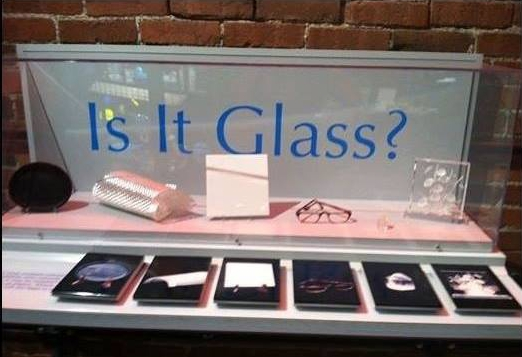
\includegraphics[width=.8\linewidth] {CarnegieGlass.jpg}
	\caption{Exhibit on display at the Carnegie Science Center (2015)}
	\label{figure:IsitGlass}
\end{figure} 

Sucrose, or common sugar, is in fact an excellent glass-forming material despite typically being encountered in its crystalline form. A familiar example of a sucrose glass—one that for many evokes childhood memory—is peanut brittle. During its preparation a mixture of sugar, corn syrup, and water is heated well above the boiling point of pure water. As boiling proceeds, water is progressively removed and the composition continuously evolves. Because water acts as a strong plasticizer for sucrose, its removal causes the glass transition temperature $T_g$ of the mixture to rise steadily throughout the cooking process.

At early stages, when the water content remains high, pulling filaments from the syrup produces strings that readily flow and collapse back into the pot. If cooled to room temperature at this stage, the mixture would form a viscous liquid rather than a glass, as its $T_g$ lies well below ambient temperature. As evaporation continues, viscosity increases dramatically and the glass transition temperature approaches room temperature. When thin filaments drawn from the pot rapidly stiffen and snap, this indicates that the evolving composition has reached a state for which cooling to ambient conditions will carry the system below its glass transition temperature. 

Thus, the critical transformation in peanut brittle is not simply cooling through $T_g$, but rather the continuous elevation of $T_g$ through removal of the plasticizing water. Pulling the syrup provides a practical means of gauging the evolving composition and determining when the material, upon cooling, will vitrify into a rigid glass rather than remain rubbery or viscous.

If you have never seen peanut brittle made, set this dissertation down for a spell and go make a batch, for in the sections that follow, we will be delving into the details of what constitutes a glass as well as the molecular dynamics of the transition from a liquid to a glassy state.  As is the case with all dissertations, beyond this introduction the material will become less colloquial and more technical.  Having a plate of peanut brittle to enjoy as you read could certainly do no harm and may even serve to bestow on you a certain experiential intuition regarding the glass transition process.  Besides, as Pamela Travers would almost certainly assert, "A glass made of sugar helps the medicine go down \nolinebreak \cite{Travers}."
	 

\section{Glasses and Glass-Forming Liquids}

Before one can have a meaningful discussion of glassy dynamics and the glass transition, one must define what constitutes a glass.  Zarzycki offers two potential definitions of glass\textemdash one operational and the other structural \nolinebreak \cite{Zarzycki}.  From an operational standpoint, one might define a glass as a liquid rapidly thermally quenched into a non-crystalline solid phase. Alternatively, from a structural perspective, a glass may be defined more generally simply as a non-crystalline solid\textemdash ignoring the means by which this state was obtained.  As Zarzycki delineates, both of these definitions fall short of providing a sufficient description of the glassy state. The simple structural perspective is too broad, encompassing materials such as gels that do not share the physical attributes of a glass. Conversely, his operational definition is too specific, omitting states that are structurally identical yet were arrived at \via means other than thermal quenching. 

Such alternative pathways include compression, which will be central to the topics of \chap \nolinebreak \ref{chap:Glycerol} and \nolinebreak \ref{chap:PCS}; pressure-induced amorphization as demonstrated by Mishima or Hemley \etal \nolinebreak \cite{Hemley,Mishima}; and cold deposition, as previously discussed regarding water ice on comets formed \via accretion \nolinebreak \cite{Debenedetti2}.  His conclusion, and the general consensus today, is that the solution lies in a definition of the glassy state which incorporates the structural perspective with the added caveat that glasses constitute a non-equilibrium solid-state system\textemdash a merger of structural and dynamic descriptions.  We will begin by examining the structural description of glasses and then proceed to consider their dynamic characteristics in detail.

\subsection{Structural Description}\label{sec:sctructualdesc}

Zarzycki's definition still requires further clarification.  Is a glass a liquid, solid, or a separate phase of matter in its own right?  One may be tempted to assert that glass is nothing more than a highly viscous liquid whose viscosity may be rapidly diverging however will still flow\textemdash albeit on a remarkably long timescale.  Indeed, one would not be hard pressed to find, even among physicists, those who believe that cathedral stained glass is thicker at the bottom of the pane due to the glass having flowed over the centuries under the influence of gravity\textemdash a very common misconception. In reality, medieval glaziers commonly installed panes with the thicker edge at the bottom for structural stability, reflecting the manufacturing process rather than viscous flow. The best models of molecular dynamics in glassy systems must be heavily extrapolated to address such timescales; nevertheless, even extremely conservative estimates place the average timescale required for these silicate glasses to flow appreciably at ambient temperatures several orders of magnitude beyond the age of the Universe \nolinebreak \cite{Zanotto}. 

In light of this, to assert that a material in a glassy state is `fluid' in any colloquial sense may seem absurd. However, one's incredulity does not a valid definition make, and one cannot dismiss the fact that a glass's radial distribution function is often indistinguishable from that of the liquid state as conceptually illustrated in \fig \nolinebreak \ref{GlassCorrComp}.

The radial distribution function, alternatively referred to as the pairwise correlation function, is a quantity defined as the expectation value of the particulate number density in a region as a function of distance from an origin placed at any arbitrarily representative particle or molecule within a bulk volume of material.  This is best conceptualized as the ensemble average of the distance between all other particles or molecules as measured from each individual particle or molecule within a bulk material.

\begin{figure}[!htbp]
	\centering
	\begin{minipage}[t]{.29\textwidth}
		\centering
		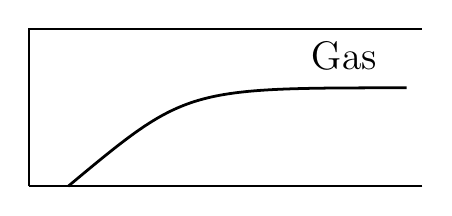
\begin{tikzpicture}	
		%Frame for plot of Gas
		\draw[thick] (0,0.25)--(0,2.25)--(5,2.25); 
		\draw[thick] (5,.25)--(0,.25);
		\draw[line width=1pt] (.5,.25) .. controls (2,1.5) .. (4.8,1.5);
		\node[] at (4,1.9) {\Large Gas};
		\end{tikzpicture}
	\end{minipage}
	\begin{minipage}[t]{.1666\textwidth}
		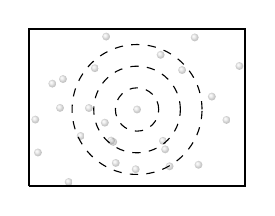
\begin{tikzpicture}	
		%Random Locations for Gas
		\foreach \y in {1,2,3,4,5}
		\foreach \x in {1,2,3,4,5}
		\shade[ball color = gray!40, opacity = 0.4] (1.325*rand+1.375,.95*rand+1.25) circle (.05cm);
		\shade[ball color = gray!40, opacity = 0.4] (1.375,1.225) circle (.05cm);
		\draw[thick] (0,0.25)--(0,2.25)--(2.75,2.25)--(2.75,.25)--(0,.25);
		\draw[dashed] (1.375,1.225) circle (.275cm);	
		\draw[dashed] (1.375,1.225) circle (.55cm);
		\draw[dashed] (1.375,1.225) circle (.825cm);		
		\end{tikzpicture}
	\end{minipage}
	\begin{minipage}[t]{.29\textwidth}
		\centering
		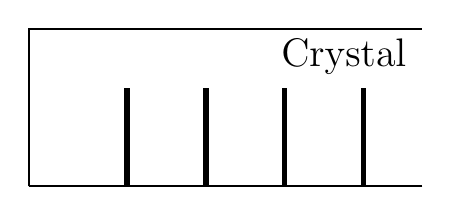
\begin{tikzpicture}	
		%Frame for plot of Crystal
		\foreach \x in {0,1,2,3}
		\draw[line width=2pt] (\x+1.25,.25)--(\x+1.25,1.5);
		\draw[thick] (0,0.25)--(0,2.25)--(5,2.25); 
		\draw[thick] (0,0.25)--(0,2.25)--(5,2.25);
		\draw[thick] (5,.25)--(0,.25);
		\node[] at (4,1.9) {\Large Crystal};
		\end{tikzpicture}
	\end{minipage}
	\begin{minipage}[t]{.1666\textwidth}
		\centering
		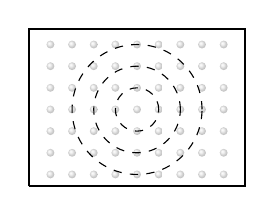
\begin{tikzpicture}	
		%Random Locations for Crystal
		\foreach \y in {1,2,3,4,5,6,7}
		\foreach \x in {1,2,3,4,5,6,7,8,9}
		\shade[ball color = gray!40, opacity = 0.4] (.275*\x,.275*\y+.125) circle (.05cm);
		\draw[thick] (0,0.25)--(0,2.25)--(2.75,2.25)--(2.75,.25)--(0,.25);
		\draw[dashed] (1.375,1.225) circle (.275cm);	
		\draw[dashed] (1.375,1.225) circle (.55cm);
		\draw[dashed] (1.375,1.225) circle (.825cm);			
		\end{tikzpicture}
	\end{minipage}
	\begin{minipage}[t]{.29\textwidth}
		\centering
		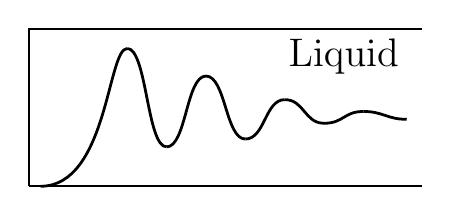
\begin{tikzpicture}	
		%Frame for plot of Liquid
		\draw[thick] (0,0.25)--(0,2.25)--(5,2.25); 
		\draw[thick] (5,.25)--(0,.25);
		\draw[line width=1pt] (.15,.25) .. controls (1,.25) and (1,2) .. (1.25,2) ;
		\draw[line width=1pt] (1.25,2) .. controls (1.5,2) and (1.5,.75) .. (1.75,.75);
		\draw[line width=1pt] (1.75,.75) .. controls (2,.75) and (2,1.65) .. (2.25,1.65) ;
		\draw[line width=1pt] (2.25,1.65) .. controls (2.5,1.65) and (2.5,.85) .. (2.75,.85) ;
		\draw[line width=1pt] (2.75,.85) .. controls (3,.85) and (3,1.35) .. (3.25,1.35) ;
		\draw[line width=1pt] (3.25,1.35) .. controls (3.5,1.35) and (3.5,1.05) .. (3.75,1.05) ;
		\draw[line width=1pt] (3.75,1.05) .. controls (4,1.05) and (4,1.2) .. (4.25,1.2) ;
		\draw[line width=1pt] (4.25,1.2) .. controls (4.5,1.2) and (4.55,1.1) .. (4.8,1.1) ;
		\node[] at (4,1.9) {\Large Liquid};
		\end{tikzpicture}
	\end{minipage}
	\begin{minipage}[t]{.1666\textwidth}
		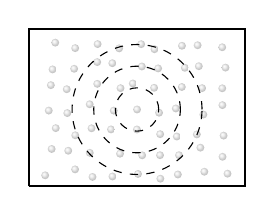
\begin{tikzpicture}	
		%Random Locations for Liquid
		\foreach \y in {1,2,3,4,5,6,7}
		\foreach \x in {1,2,3,4,6,7,8,9}
		\shade[ball color = gray!40, opacity = 0.4] (.275*\x+.275*rand/4,.275*\y+.275*rand/4+.125) circle (.05cm);
		\foreach \y in {1,2,3,5,6,7}
		\shade[ball color = gray!40, opacity = 0.4] (1.375+.275*rand/4,.275*\y+.275*rand/4+.125) circle (.05cm);	
		\shade[ball color = gray!40, opacity = 0.4] (1.375,1.225) circle (.05cm);		
		\draw[thick] (0,0.25)--(0,2.25)--(2.75,2.25)--(2.75,.25)--(0,.25);
		\draw[dashed] (1.375,1.225) circle (.275cm);	
		\draw[dashed] (1.375,1.225) circle (.55cm);
		\draw[dashed] (1.375,1.225) circle (.825cm);		
		\end{tikzpicture}
	\end{minipage}
	\begin{minipage}[t]{.29\textwidth}
		\centering
		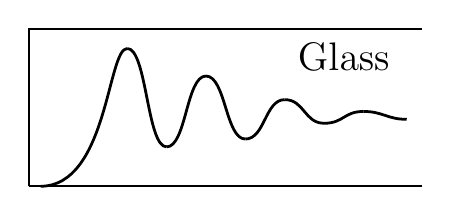
\begin{tikzpicture}	
		%Frame for plot of Gass
		\draw[thick] (0,0.25)--(0,2.25)--(5,2.25); 
		\draw[thick] (5,.25)--(0,.25);
		\draw[thick] (0,0.25)--(0,2.25)--(5,2.25); 
		\draw[thick] (5,.25)--(0,.25);
		\draw[line width=1pt] (.15,.25) .. controls (1,.25) and (1,2) .. (1.25,2) ;
		\draw[line width=1pt] (1.25,2) .. controls (1.5,2) and (1.5,.75) .. (1.75,.75);
		\draw[line width=1pt] (1.75,.75) .. controls (2,.75) and (2,1.65) .. (2.25,1.65) ;
		\draw[line width=1pt] (2.25,1.65) .. controls (2.5,1.65) and (2.5,.85) .. (2.75,.85) ;
		\draw[line width=1pt] (2.75,.85) .. controls (3,.85) and (3,1.35) .. (3.25,1.35) ;
		\draw[line width=1pt] (3.25,1.35) .. controls (3.5,1.35) and (3.5,1.05) .. (3.75,1.05) ;
		\draw[line width=1pt] (3.75,1.05) .. controls (4,1.05) and (4,1.2) .. (4.25,1.2) ;
		\draw[line width=1pt] (4.25,1.2) .. controls (4.5,1.2) and (4.55,1.1) .. (4.8,1.1) ;
		\node[] at (4,1.9) {\Large Glass};
		\end{tikzpicture}
	\end{minipage}
	\begin{minipage}[t]{.1666\textwidth}
		\centering
		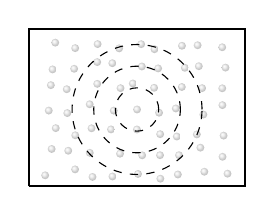
\begin{tikzpicture}	
		%Random Locations for Glass
		\foreach \y in {1,2,3,4,5,6,7}
		\foreach \x in {1,2,3,4,6,7,8,9}
		\shade[ball color = gray!40, opacity = 0.4] (.275*\x+.275*rand/4,.275*\y+.275*rand/4+.125) circle (.05cm);
		\foreach \y in {1,2,3,5,6,7}
		\shade[ball color = gray!40, opacity = 0.4] (1.375+.275*rand/4,.275*\y+.275*rand/4+.125) circle (.05cm);	
		\shade[ball color = gray!40, opacity = 0.4] (1.375,1.225) circle (.05cm);		
		\draw[thick] (0,0.25)--(0,2.25)--(2.75,2.25)--(2.75,.25)--(0,.25);
		\draw[dashed] (1.375,1.225) circle (.275cm);	
		\draw[dashed] (1.375,1.225) circle (.55cm);
		\draw[dashed] (1.375,1.225) circle (.825cm);		
		\end{tikzpicture}
	\end{minipage}
	\caption{Typical radial correlation functions for a gas, liquid, glass, and crystal.  This figure is derivative of that originally published by Johari. \cite{Johari}} \label{GlassCorrComp} 
\end{figure}

Significantly simplified two-dimensional representations of radial distribution functions and the structures giving rise to them for a gas, liquid, crystal, and glass are provided in the aforementioned \fig \nolinebreak \ref{GlassCorrComp}.  Note that the exact particle locations for this figure were determined implementing a random number generator and thus are not representative of the ensemble average resulting from any specific intermolecular potential.  This figure is relevant to a discussion of the characteristics typical of pairwise correlation functions for these four material states only in the most general of terms.  The two-dimensional analog of a crystalline structure is shown in greater detail here in \fig \nolinebreak \ref{distributionDefined} where the characteristic radii between horizontally and vertically adjacent particles are labeled $r_1$.  The characteristic radii corresponding to the nearest neighbor, next nearest neighbor, and next-next nearest neighbor are labeled $r_1$, $r_2$ and $r_3$ respectively.  These will exhibit rapidly decreasing correlation amplitudes for higher order nearest neighbors.  The corresponding radial distribution function exhibits very sharp periodic peaks associated with these infinitely repeating lattice spacings.  The exact appearance of a radial distribution function for any real crystalline bulk material can clearly be quite complex and will vary from one material to the next as it depends directly upon the crystal symmetry, however it will always consist of such well defined periodic peaks.  The arguably oversimplified crystalline pair correlation spectra shown in \fig \nolinebreak \ref{GlassCorrComp} ignores all peaks associated with these off diagonal contributions from the lattice structure to provide an even further conceptually idealized spectra.  Strictly speaking, such a simple correlation spectra could only ever arise from a one dimensional distribution of evenly spaced particles however it represents the behavior of a repetitive lattice structure sufficiently well for the purposes of this discussion, and in fact it is not uncommon for solid-state physics texts to similarly describe the band structure along a single direction of a 3D crystalline structure.

\begin{figure} [!htbp]
	\centering
	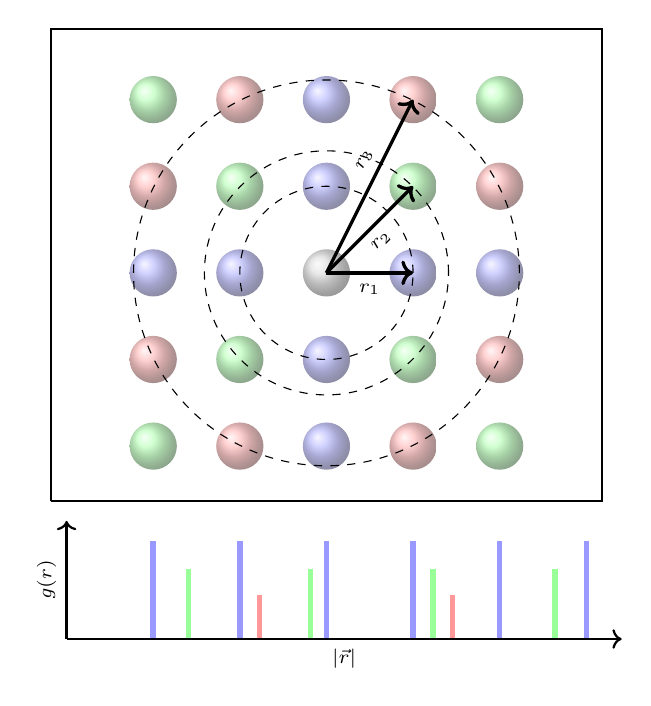
\begin{tikzpicture}	
	%Top Row of Particles
	\foreach \x in {3,7}
	\shade[ball color = green!40, opacity = 0.6] (1.1*\x,1.1*6+.5) circle (.3cm);
	\foreach \x in {4,6}
	\shade[ball color = red!40, opacity = 0.6] (1.1*\x,1.1*6+.5) circle (.3cm);
	\shade[ball color = blue!40, opacity = 0.6] (1.1*5,1.1*6+.5) circle (.3cm);
	
	%2nd Row of Particles
	\foreach \x in {3,7}
	\shade[ball color = red!40, opacity = 0.6] (1.1*\x,1.1*5+.5) circle (.3cm);
	\foreach \x in {4,6}
	\shade[ball color = green!40, opacity = 0.6] (1.1*\x,1.1*5+.5) circle (.3cm);
	\foreach \x in {5}
	\shade[ball color = blue!40, opacity = 0.6] (1.1*\x,1.1*5+.5) circle (.3cm);
	
	%3rd Row of Particles
	\foreach \x in {3,4,6,7}
	\shade[ball color = blue!40, opacity = 0.6] (1.1*\x,1.1*4+.5) circle (.3cm);
	
	%4th Row of Particles
	\foreach \x in {3,7}
	\shade[ball color = red!40, opacity = 0.6] (1.1*\x,1.1*3+.5) circle (.3cm);
	\foreach \x in {4,6}
	\shade[ball color = green!40, opacity = 0.6] (1.1*\x,1.1*3+.5) circle (.3cm);
	\foreach \x in {5}
	\shade[ball color = blue!40, opacity = 0.6] (1.1*\x,1.1*3+.5) circle (.3cm);
	
	%Bottom Row of Particles
	\foreach \x in {3,7}
	\shade[ball color = green!40, opacity = 0.6] (1.1*\x,1.1*2+.5) circle (.3cm);
	\foreach \x in {4,6}
	\shade[ball color = red!40, opacity = 0.6] (1.1*\x,1.1*2+.5) circle (.3cm);
	\foreach \x in {5}
	\shade[ball color = blue!40, opacity = 0.6] (1.1*\x,1.1*2+.5) circle (.3cm);
	
	%Central Ball in Red
	\shade[ball color = gray!40, opacity = 0.6] (1.1*5,1.1*4+.5) circle (.3cm);
	
	%Outline
	\draw[thick] (2,2)--(2,8)--(9,8)--(9,2)--(2,2);
	\draw[dashed] (5.5,4.9) circle (1.1cm);		
	\draw[dashed] (5.5,4.9) circle (1.55cm);	
	\draw[dashed] (5.5,4.9) circle (2.45cm);	
	\draw[->,very thick,black] (5.5,4.9)--(6.6,4.9) node[draw=none,fill=none,font=\scriptsize,midway,below] {$r_1$};
	\draw[->,very thick,black] (5.5,4.9)--(6.6,1.1*5+.5) node[draw=none,fill=none,font=\scriptsize,midway,below,rotate =45] {$r_2$};
	\draw[->,very thick,black] (5.5,4.9)--(6.6,1.1*6+.5)
	node[draw=none,fill=none,font=\scriptsize,anchor=south west,midway,rotate =63.435] {$r_3$};
	
	
	%Primary Peaks
	\foreach \x in {1,2,3,4,5,6}
	\draw[line width=2pt,color = blue!40] (2.2+\x*1.1,.25)--(2.2+\x*1.1,1.5);
	%First Harmonic
	\foreach \x in {1,2,3,4}
	\draw[line width=2pt,color = green!40] (2.2+\x*1.55,.25)--(2.2+\x*1.55,1.13388);
	%Third Harmonic
	\foreach \x in {1,2}
	\draw[line width=2pt,color = red!40] (2.2+\x*2.45,.25)--(2.2+\x*2.45,.809);
	%Radial Distribution Function
	\draw[->,thick] (2.2,0.25)--(9.25,.25) node[draw=none,fill=none,font=\scriptsize,midway,below,rotate =0] {$\left | \vec{r} \right |$};; 
	\draw [->,thick] (2.2,0.25) -- (2.2,1.75) node[draw=none,fill=none,font=\scriptsize,midway,above,rotate =90] {$g(r)$};
	
	
	\end{tikzpicture}  \caption{A crystalline solid exhibits one or more characteristic radii, for which adjacent individual particles or molecules appear at integer multiples.  The corresponding radial distribution function for such a material will consist of sharp periodic peaks.} \label{distributionDefined} 
\end{figure} 

Conversely, gases exhibit no such periodic order.  Due to the strong yet exceedingly short range Coulombic repulsion, molecules will spend very little time in extremely close proximity, existing mostly in a free state where intermolecular interactions are negligible.  As such, their pairwise correlation function will very rapidly approach a uniform value corresponding to the average particle density.  An idealized representation of this is provided in the top left window of \fig \nolinebreak \ref{GlassCorrComp}.

From a structural perspective, both liquids and glasses will exhibit radial distributions functions that appear almost as if they consisted of a damped superposition of the gas and crystalline states.  This arises due to the fact that the intermolecular interactions between the constituent molecules of both liquids and glasses are not negligible.  Short-range order emerges as bonds between adjacent constituent molecules are formed.  As this order is at the same time imperfect relative to the crystalline structure, short range, and in the case of a liquid also of short duration, it will manifest itself in the broadening and dampening of the periodic peaks of the corresponding pairwise correlation function.  Representative idealized liquid and glass radial distribution functions are provided in \fig \nolinebreak \ref{GlassCorrComp} as well.  Note the periodic peaks that correspond to an imperfect crystalline structure in short order giving way to an utter lack of long range order indicative of a gas\textemdash albeit at significantly higher density.  

Similarities between the radial correlation functions for a liquid and a glass are worthy of note. Structurally, they are nearly\textemdash if not entirely\textemdash identical. However, they differ vastly in their dynamics. For a liquid, the radial correlation function can be thought of either as arising from a time average of the molecular positions or, equivalently, from an ensemble average calculated from the positions of all individual particles at a single instant in time. Conversely, the dynamics of a glass—being an amorphous solid—are such that its radial correlation function is best understood solely in terms of an ensemble average, since constituent molecules do not move appreciably on experimentally meaningful timescales. Thus, we encounter the curious condition of two material states possessing identical structure yet fundamentally different dynamics. Having explored the structural similarities and differences between glasses and liquids, we now turn our attention to their dynamic properties, particularly how these dynamics reflect differences in molecular motion and energy landscapes.

\subsection{Dynamic Description}

Molecules in a gas state have high enough energy on average that they do not really "feel" the potential energy landscape produced by their neighbors.  They take on a relatively random and highly degenerate spatial distribution where intermolecular interactions are limited to the strong yet exceedingly short range Coulombic repulsion of their electronic shells.  Thus the pairwise correlation function for a well thermalized gas will exhibit very little structure beyond a rapid increase in correlation, arising from this Coulombic repulsion repelling other molecules at close proximity, quickly leveling off to a region of constant number density, beyond the influence of this repulsive force, that will extend indefinitely as demonstrated in \fig \nolinebreak \ref{GlassCorrComp}.

Gases and crystals are, in this sense, polar opposite scenarios in that the former has sufficient thermal energy that the potential landscape arising from the intermolecular forces is almost irrelevant as molecules spend very little time in close enough proximity to any other molecule for even the dominant Coulombic interaction to play a major role in their dynamics, yet the latter has sufficiently low thermal energy such that dynamics are dominated by intermolecular forces beyond Coulombic repulsion\textemdash higher order terms such as dipole or other types of interactions depending on the nature of the constituent atoms making up the crystal.  Molecules in a crystalline state certainly \textit{feel} their potential energy landscape, yet are not free to explore it as most of that parameter space is energetically inaccessible. Thus they are locked into discrete, highly symmetric arrangements associated with the lowest energy structural state of the bulk system. These are the two extremes of which the liquid state is an intermediate.  

Within the energetically intermediate liquid state, molecules or particles have sufficient energy to explore their potential energy landscape yet still be heavily influenced, and to some extent confined, by said landscape.  Short lived bonds between molecules form, increasing the average time in which they are in close proximity and giving rise to cooperative motion.  However these nearest neighbor bonds \textit{are} very short lived\textemdash the activation energy required to break the bonds being on the order of the thermal energy, $k_BT$, of the material. The bonds conforming to the lowest energy orientations corresponding to the crystalline structure, though not exclusively occurring, will clearly be statistically favored.  Thus liquids exhibit the rapid emergence, and subsequent disintegration, of short-range order that may be described as spatially distorted crystalline arrangements.  One would expect that the radial distribution function of a liquid will therefore exhibit structures that resemble the crystalline peaks over a short range, though broadened due to thermal motion and the absence of long-range positional order. However, over sufficiently large separations, these short-lived local nucleations bear no correlation from one region to the next and, as such, the radial correlation function for a liquid approaches unity at large radii\textemdash reflecting the absence of long-range order while maintaining the characteristic number density of the liquid phase. The radial correlation function for a liquid displayed in \fig \nolinebreak \ref{GlassCorrComp} shows what would be expected for a state that is intermediate between a gas and a crystalline solid, \ie, broadened crystalline peaks at short range that quickly wash out to a uniform average number density at larger radii.

Another way to describe the liquid state of a glass-forming system, beyond purely energetic considerations, is to consider the timescales on which the potential energy landscape is explored by the system\textemdash \ie, its structural relaxation time. It should be noted that a variety of relaxation processes occur in any glassy system, not all of which are directly associated with the bulk structural rearrangement. These include thermal relaxations as well as processes arising from diffusion and orientational dynamics, the complexity of which depends strongly on the internal degrees of freedom available to the constituent molecules. 

Even relatively simple glass formers typically exhibit two broad dynamical regimes: fast $\beta$-relaxations, which generally display relatively little dependence on temperature and pressure, and the $\alpha$ relaxation process, which is highly sensitive to thermodynamic conditions and may vary by thirteen or more orders of magnitude between the high-temperature or low-pressure liquid and the glassy state. The $\alpha$ relaxation is the structural relaxation mode of the system, associated with the cooperative motion of many nearby particles and involving mechanisms such as the breaking of nearest-neighbor cages, molecular reorientation, and diffusive rearrangement. It is this structural $\alpha$ relaxation process that is the focus of this dissertation.

In the following section we will discuss several probes of these relaxation dynamics, including Photon Correlation Spectroscopy in \sect\nolinebreak \ref{sec:PCSintro}.  Time-domain correlation spectra obtained using this technique on glass-forming systems are generalized in \fig \nolinebreak \ref{figure:RelaxationShiftIntro} to illustrate this dynamic behavior under varying thermodynamic conditions.  Here, the correlation time, $\tau$, is simply the average time required for a bulk material to relax having been subjected to some form of mechanical perturbation\textemdash  inherently tied to the imaginary component of the bulk modulus. Generally speaking, the fast $\beta$-relaxation will be relatively unaffected by changing thermodynamic parameters.  However, as the temperature of a liquid decreases or, equivalently, as pressure increases, the $\alpha$ relaxation time increases continuously over many orders of magnitude. In the high-temperature or low-pressure liquid, $\tau_{\alpha}$ is typically on the order of picoseconds, whereas at the glass transition it reaches approximately $10^{2}$ seconds. The rate at which $\tau_{\alpha}$ varies with temperature or pressure depends strongly on the fragility of the liquid, with fragile systems exhibiting especially pronounced changes as $T_g$ is approached, while strong liquids display a more gradual evolution.  Understanding how this structural relaxation time grows as thermal energy is reduced or free volume is diminished under compression is central to describing the nature of the glass transition.

	\pgfplotsset{table/search path={Chapters/Background/Figures},}
\begin{figure}[!htbp]
	\centering
	\begin{tikzpicture} 
		\begin{axis}[
			height=.5\textwidth,
			width=.75\textwidth,
			ylabel={$\left \langle A\left ( 0 \right )A\left ( \tau \right ) \right \rangle$},
			xlabel={Correlation Time ($\tau$)},
			xmin=1E-12, xmax=1E4,
			ymin=0, ymax=1,
			xtick={1E-12,1E-10,1E-8,1E-6,1E-4,1E-2,1E0,1E2,1E4},
			ytick={0.2,0.4,0.6,0.8,1},
			xmode=log,
			ymajorgrids=false,
			grid style=dashed,
			legend style={at={(0.225,.425)}},
			legend image post style={mark=none}
			]
			
			\draw[<-,thick] (1E-11,.9)--(1E-10,.9);
			\node[anchor=west] at (1E-10,.9) {$\beta$-relaxation};
			\draw[->,thick] (5E-8,.6)--(5E-7,.6);
			\node[anchor=east] at (5E-8,.6) {$\alpha$-relaxation};
			\draw[->,very thick] (1E1,.9)--(1E3,.9);
			\node[anchor=south east] at (1E1,.9) {$P \uparrow$};
			\node[anchor=east] at (1E1,.85) {$T \downarrow$};
			
			% Shortest relaxation time (fast liquid)
			\addplot [black, very thick, solid] 
			table [x=time, y=1micro, col sep=comma] {Relaxations.csv};
			\addlegendentry{{\scriptsize 1.00 \;\si{\micro\second}}}
			
			\addplot [black, thick, densely dashed] 
			table [x=time, y=100micro, col sep=comma] {Relaxations.csv};
			\addlegendentry{{\scriptsize 100 \;\si{\micro\second}}}
			
			\addplot [black, semithick, dashed] 
			table [x=time, y=10milli, col sep=comma] {Relaxations.csv};
			\addlegendentry{{\scriptsize 10 \;\si{\milli\second}}}
			
			\addplot [black, semithick, dashdotted] 
			table [x=time, y=1sec, col sep=comma] {Relaxations.csv};
			\addlegendentry{{\scriptsize 1.00 \;\si{\second}}}
			
			% Longest relaxation time (near Tg)
			\addplot [black, dotted] 
			table [x=time, y=100sec, col sep=comma] {Relaxations.csv};
			\addlegendentry{{\scriptsize 100 \;\si{\second}}}
			
		\end{axis} 
	\end{tikzpicture}
	\caption{An idealized set of autocorrelation curves typical of what might be obtained for a glass-forming system. The characteristic structural relaxation time $\tau_\alpha$ falls near the foot of each curve. As temperature is decreased or pressure is increased, the faster $\beta$-relaxation remains relatively fixed; however, the $\alpha$-relaxation shifts to longer times as structural relaxation slows and an increasing fraction of the energy landscape becomes energetically inaccessible.}  
	\label{figure:RelaxationShiftIntro}
\end{figure}

In the most simplistic of terms, glassy materials exhibit the rigidity of a crystalline state, having insufficient thermal energy to readily explore their potential energy landscape, yet maintain the semi-ordered structure of their liquid state.  Their radial correlation functions, as characterized in \fig \nolinebreak \ref{GlassCorrComp}, will be very similar in structure to that of the liquid state, often exhibiting short range crystalline structure albeit with copious irregularities, transitioning into rapidly diminishing structural correlation over longer distances.  A very marked difference between a system in a liquid \vs a glassy state is the apparent violation of ergodicity.  Although the radial correlation function of a glass may be similar to the liquid state in general structure, it may not be quite as identical as implied by \fig \nolinebreak \ref{GlassCorrComp}.  Glassy systems will exhibit mechanical hysteresis stemming from their exceedingly slow structural relaxations. This along with the lower thermal energy of these systems results in intermolecular bonds being much longer lived than in the liquid state which may lead to semi-crystalline domains growing quite large.  Cooperative motion of these domains will play a much greater role in the dynamics of glassy systems than in a liquid state.  These considerations, among others, leave open the question as to whether glass exists as a separate phase of matter or as nothing more than a highly viscous fluid\textemdash a question we will now address.  

\section{The Nature of the Glass Transition}

A material undergoing a change in phase will experience a dramatic and discontinuous shift in bulk properties such as density, specific heat, bulk modulus, thermal expansivity, \etc  Ehrenfest more precisely defined phase transitions as points in the pressure-temperature-volume phase space of the material where discontinuities in the derivatives of the Gibbs free energy with respect to any external thermodynamic parameter emerge.  Transitions between any two states described in \fig \nolinebreak \ref{GlassCorrComp} with the exception of the glass transition will constitute what Ehrenfest described as a first-order phase transition in that it will involve discontinuities in first-order derivatives of the free energy, or equivalently enthalpy, for a transition at constant pressure \nolinebreak \cite{Jaeger}.  The glass transition, however, is distinct from the others in that no such first-order discontinuity exists.  \fig \nolinebreak \ref{figure:Transition} shows the plot of enthalpy or specific volume as a function of temperature for an idealized glass-forming system maintained at constant pressure.  At the freezing temperature, $T_f$, the enthalpy of fusion—equivalently the latent heat of fusion—corresponds to a discontinuous change in enthalpy. Such a discontinuity in the first derivative of the Gibbs free energy is the defining characteristic of a first-order phase transition and is apparent in \fig \nolinebreak \ref{figure:Transition}. In principle, any liquid capable of forming a crystalline structure, if brought to this temperature, provided with a single nucleation point, and allowed to cool slowly enough to maintain thermalization, will form a single-crystal solid that constitutes the global minimum on the potential energy landscape as represented in \fig \nolinebreak \ref{figure:landscape}.  This conceptually idealized projection of the potential energy landscape, adapted from the review by Debenedetti and Stillinger \cite{Debenedetti}, represents the potential energy as a function of a single configurational coordinate. It is, obviously, not possible to aptly describe the potential landscape for any real system graphically as it will span a parameter space whose dimension will be on the order of the number of constituent molecules residing in the bulk multiplied by their individual degrees of freedom.  However this overly simplified single dimensional representation is quite sufficient as a conceptual illustration.  

\begin{figure} [!htbp] 
	\centering
	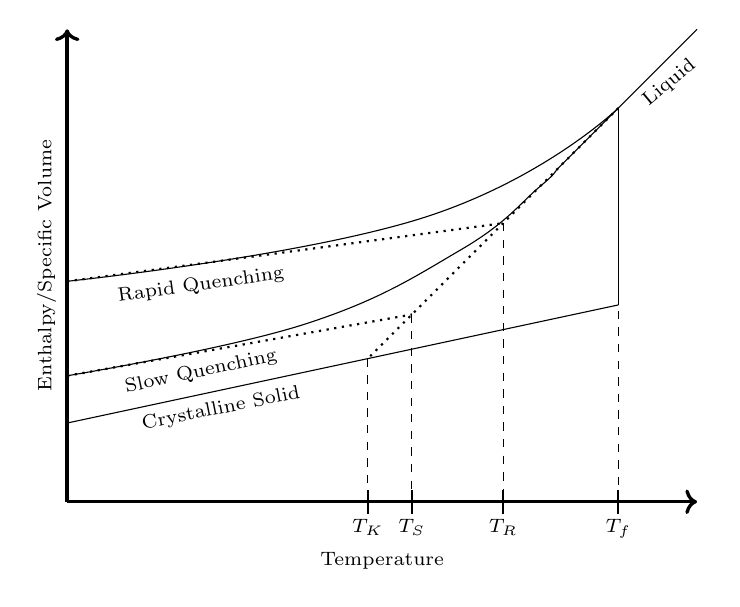
\begin{tikzpicture}
		\draw[very thick,->] (0,0)--(0,6) node[draw=none,fill=none,font=\scriptsize,midway,above,rotate =90] {Enthalpy/Specific Volume};
		\draw[very thick,->] (0,0)--(8,0); \node[draw=none,fill=none,font=\scriptsize] at (4,-.75) {Temperature};
		
		\draw[] (0,1)--(3.81818,1.81818)
		node[draw=none,fill=none,font=\scriptsize,midway,below,rotate = 11.31] {Crystalline Solid};
		\draw[] (3.81818,1.81818)--(7,2.5);
		\draw[] (7,2.5)--(7,5);
		\draw[] (7,5)--(8,6)
		node[draw=none,fill=none,font=\scriptsize,midway,below,rotate = 39.81] {Liquid};
		\draw[dotted, thick] (7,5)--(3.81818,1.81818); 
		
		\draw[thick] (7,-0.15)--(7,0.15);
		\draw[dashed] (7,0)--(7,2.5);
		\node[draw=none,fill=none,font=\scriptsize,below] at (7,-.1) {$T_f$};
		
		\draw  plot[smooth, tension=.7] coordinates {(7,5) (6.75,4.75) (6.5,4.5) (6.25,4.25) (6,4) (5,3.2) (3,2.25) (0,1.6)};
		\node[draw=none,fill=none,font=\scriptsize,rotate = 12] at (1.7,1.65) {Slow Quenching};
		\draw  plot[smooth, tension=.8] coordinates {(7,5) (4.5,3.6) (0,2.8)};
		\node[draw=none,fill=none,font=\scriptsize,rotate = 8] at (1.7,2.75) {Rapid Quenching};
		
		\draw[thick] (5.53846,-0.15)--(5.53846,0.15);
		\draw[dotted,thick] (0,2.8) -- (5.53846,3.53846);
		\draw[dashed] (5.53846,3.53846)--(5.53846,0);
		\node[draw=none,fill=none,font=\scriptsize,below] at (5.53846,-.1) {$T_{R}$};	
		\draw[thick] (4.37838,-0.15)--(4.37838,0.15);
		\draw [dotted,thick] (-0,1.6) -- (4.37838,2.37838);
		\draw [dashed] (4.37838,2.37838)--(4.37838,0);
		\node[draw=none,fill=none,font=\scriptsize,below] at (4.37838,-.1) {$T_{S}$};	
		\draw[thick] (3.81818,-0.15)--(3.81818,0.15);
		\draw [dashed] (3.81818,1.81818)--(3.81818,0);
		\node[draw=none,fill=none,font=\scriptsize,below] at (3.81818,-.1) {$T_{K}$};	
	\end{tikzpicture}
	
\caption{An idealized representation of a typical plot obtained \via differential scanning calorimetry to determine the glass transition \cite{ONeill}. The smooth crossover from the linear trend of the liquid state to that of the glassy state, exaggerated here for clarity, would be expected in the absence of any higher-order transition in the Ehrenfest sense. The dashed lines indicate extrapolations of the equilibrium liquid branch at temperatures sufficiently above $T_g$ and of the amorphous solid branch at temperatures sufficiently below $T_g$ for glasses formed \via rapid and slow thermal quenching. The Kauzmann temperature for the limiting case is also shown, as it motivates the argument that such smooth extrapolations may be non-physical.}
\label{figure:Transition}
\end{figure}

If cooled below the freezing temperature while crystallization is suppressed, the enthalpy will continue to decrease with the removal of internal energy and accompanying thermal contraction until, in the limit of absolute zero, only a single energetically accessible state remains, corresponding to zero entropy.  This stands in stark contrast to a glassy state where a certain degree of entropy, associated with structural disorder, is locked in.  This can occur when a liquid is thermally quenched very rapidly.  Rapidly, in this context, implies that thermal energy is removed quickly enough that the system cannot thoroughly explore its potential energy landscape. Consequently, it becomes trapped in metastable local minima, failing to reach the global minimum associated with the crystalline ground state.  \fig \nolinebreak \ref{figure:landscape} labels one such local minimum as an ``ideal glass.'' It should be emphasized, however, that while the crystalline state represents the unique global minimum of the potential energy landscape, this landscape itself depends on the positions and orientations of all constituent particles and is therefore extraordinarily complex. It contains an immense number of local minima, any of which may trap a rapidly quenched system. The ``ideal glass'' is thus understood as a particular deeply trapped metastable minimum rather than the true thermodynamic ground state. Many of the local minima correspond to metastable basins separated by finite energy barriers. Transition states, properly understood as saddle points between adjacent minima, are unstable along at least one configurational direction and mediate transitions between these metastable states. Supercooled liquids occupy such metastable basins, separated by finite energy barriers. A familiar example is sodium acetate heat packs, which remain in a metastable liquid state until a small perturbation triggers rapid crystallization. Some systems do not so readily crystallize and, upon rapid thermal quenching, settle into an amorphous solid locked within a local energy minimum that rests above that of the crystalline state, but significantly below what would be considered a transition state. For such a system, the entropy does not approach zero as enthalpy decreases because the energy landscape contains an enormous number of distinct metastable basins of comparable depth. Upon rapid quenching, the system becomes confined within one such basin—microscopically reflected in molecules trapped within nearest-neighbor cages—but the multiplicity of alternative basins gives rise to a residual configurational entropy. The barriers separating these basins are sufficiently large that inter-basin transitions are effectively suppressed on experimental timescales.

\graphicspath{{Chapters/Background/Figures/}}
\begin{figure} [!htbp]
	\centering
	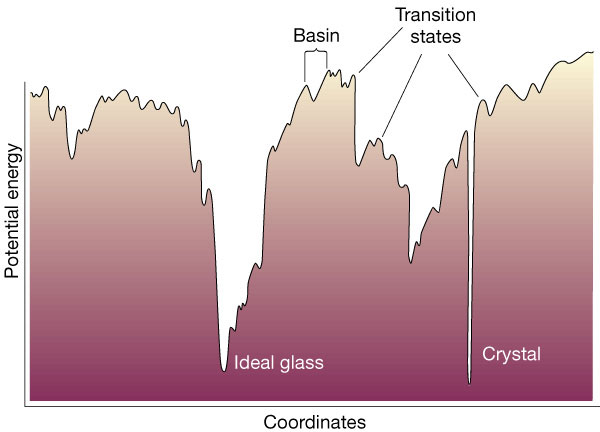
\includegraphics[width=.8\linewidth] {landscape.jpg}
	\caption{The two dimensional representation of an energy landscape for an idealized glass-forming system provided by Debenedetti and Stillinger \cite{Debenedetti}.}
	\label{figure:landscape}
\end{figure}

This is the glass transition and is perhaps well described again by \fig \nolinebreak \ref{figure:Transition} where the discontinuity in first order derivatives of the free energy are not present but rather a rapid yet smooth transition does occur as temperature decreases.  The nature of the glass transition—whether it constitutes a legitimate second-order phase transition or simply reflects rapid vitrification of the liquid state—could, in principle, be experimentally resolved in this context. If the transition is indeed smooth, lacking any discontinuity in higher-order derivatives, then the glass “transition” is merely a kinetic effect associated with a rapidly vitrifying liquid. However, if the smooth crossover implied by \fig \nolinebreak \ref{figure:Transition} does not accurately reflect the true behavior and instead a discrete discontinuity in slope exists, then the glass transition represents more than rapid vitrification; it would constitute a second-order transition in the Ehrenfest sense into a distinct thermodynamic state. Such measurements, however, do not readily provide the precision necessary to resolve a discontinuity of this kind conclusively. Nevertheless, there remains a compelling argument for the necessity of a second-order transition consistent with the observed thermodynamic behavior of glass-forming systems.

Assume for a moment that the glass "transition" is a purely kinetic vitrification process.  As depicted in \fig \nolinebreak \ref{figure:Transition}, upon super-cooling below the freezing point, $T_m$, enthalpy or specific volume will quickly approach a trend that tracks with that of the crystalline solid yet will remain systematically above the corresponding values of the crystal enthalpy as temperature continues to decrease. The exact values of enthalpy, specific volume, heat capacity, or many other bulk properties of the glassy material will depend on its thermal history including how rapidly it was quenched.  Extremely rapid thermal quenching may result in a much less ordered glassy system as molecules have virtually no time to seek out even relatively pronounced local minimums on the potential surface.  Slightly slower quenching may allow local order to arise thus giving bulk properties closer to that of the crystalline state.  For a first order phase transition, such as from a liquid to a crystalline solid, there is a specific well defined temperature at which this transition occurs.  It is desirable to define such a transition temperature for the glass transition as well.  One such definition is demonstrated in \fig \nolinebreak \ref{figure:Transition} as the intersection of the extrapolations of the linear trends in Enthalpy or specific volume as a function of temperature from well within the glassy state and from the supercooled liquid state.  These extrapolations are shown as dotted lines in \fig \nolinebreak \ref{figure:Transition} and their intersections marked as vertical dashed lines corresponding to the characteristic transition temperatures, $T_S$ and $T_R$, for a glass-forming system undergoing slow and rapid thermal quenching, respectively.  These points of intersection clearly cannot suffice as a definition for the glass transition temperature, $T_g$,  as they will inherently constitute a range of values strongly dependent upon the rate of cooling as, from an energy landscape perspective, the rate of cooling will determine to what extent the constituent molecules have time to explore the energy landscape before becoming energetically locked into a local minimum corresponding to a glassy state associated with a specific local minimum on the potential energy landscape. The more rapidly a system is quenched the more likely it is to be locked into a state that is energetically much further from the crystalline state as well as having a significantly higher residual entropy as temperature approaches absolute zero corresponding to the higher level of structural disorder.  A standard metric experimental protocol must be agreed upon if one is to define a singular glass transition temperature, $T_g$.  The most common method of defining $T_g$, at least at atmospheric pressure, has been \via calorimetric measurements which directly probe the heat capacity of the liquid as temperature is scanned at a controlled, generally agreed upon rate through the glass transition\textemdash typically ten Kelvin per minute.  At these rates a value of $T_g$ is found consistently to correspond to viscosities on the order of $10^{13}$ poise or an $\alpha-$relaxation time on the order of $100$ seconds \nolinebreak \cite{Stebbins}.  The temperatures associated with these viscosities or characteristic structural relaxation times have been generally accepted as the standard definition of the glass transition temperatures, $T_g$, throughout the literature and are those to which this work will conform.  Further details of calorimetric methods will not be  described here as these methods do not prove practical at very high pressures and were not implemented to obtain any of the data appearing in this work.  However, this thermodynamic description of the glass transition remains pertinent as it illustrates, quite effectively, one argument for the glass transition being a second order phase transition, as opposed to a purely kinematic process of rapid vitrification as will now be discussed.  

The curve labeled "Slow Quenching" in \fig \nolinebreak \ref{figure:Transition} is not, in any strict sense, a limiting case for a given glass-forming material; in principle, one may always cool more slowly. In practice, spontaneous nucleation events often induce crystallization in supercooled liquids, as observed in systems such as propylene carbonate and salol \nolinebreak \cite{Szklarz}. Similar spontaneous crystallization has also been observed in our laboratory in super-pressed salol under high-pressure conditions, where a crystalline front advanced gradually across the sample on timescales of days. However, for strong glass-formers, bulk crystallization can be suppressed even under extremely slow cooling rates.

Under such conditions, one may instead envision the formation of increasingly large locally ordered domains distributed throughout the material. These domains can progressively restrict the mobility of neighboring regions, ultimately arresting long-range structural rearrangement and producing a glassy state. The microscopic mechanisms that frustrate large-scale crystallization remain an active area of investigation \nolinebreak \cite{Shintani}.

If cooling could proceed arbitrarily slowly while still avoiding macroscopic crystallization, the bulk thermodynamic properties would be expected to approach those of the crystalline state. Extrapolation of the linear trend shown in \fig \nolinebreak \ref{figure:Transition} would then imply that the enthalpy or specific volume of the liquid could fall below that of the crystal. Such behavior would correspond to a state possessing lower entropy than the crystalline phase—an outcome known as the Kauzmann paradox \nolinebreak \cite{Kauzmann}. 

Because this scenario is thermodynamically untenable, the approach to the crystalline state must either remain asymptotic or be interrupted by a phase transition. Gibbs and DiMarzio proposed that a true second-order Ehrenfest transition could occur at the Kauzmann temperature, $T_K$, thereby resolving the paradox \nolinebreak \cite{GibbsandDiMarzio,Gibbs2}. Experimentally, however, spontaneous crystallization typically intervenes before $T_K$ can be reached, preventing direct verification of this proposal.

The argument outlined above highlights a long-standing temptation within the glass literature\textemdash namely, to interpret the apparent approach toward the Kauzmann temperature as evidence for an underlying thermodynamic phase transition. In many theoretical treatments, this transition is hypothesized to occur either at an extrapolated temperature such as $T_K$ or, in some frameworks, at a temperature above $T_g$ that would mark the onset of distinct glassy order. Mean-field and random first-order transition models, for example, predict such behavior under certain assumptions. Moreover, in disordered systems such as spin glasses, genuine thermodynamic phase transitions are well established. The situation for structural glasses, however, remains less definitive. At present, the experimental evidence does not conclusively establish whether the structural glass transition\textemdash at $T_g$, above it, or at any extrapolated temperature such as $T_K$\textemdash corresponds to a true thermodynamic phase transition.

The persistence of the higher-order interpretation stems in part from an extrapolative paradox whose logical structure bears resemblance to Zeno’s famous paradox of motion. In Zeno’s construction, a traveler attempting to reach a wall must first traverse half the distance, then half of the remaining distance, and so on \emph{ad infinitum}. Because this reasoning generates an infinite sequence of steps, it appears to forbid arrival. The flaw, of course, lies not in the subdivision of space, but in neglecting the dynamics of the process: at finite velocity, each successive interval requires half the time of the previous one, and the total traversal time forms a convergent geometric series. Once the temporal structure is properly accounted for, the paradox dissolves.

The Kauzmann paradox may be viewed as an inverted analogue of this reasoning. If one assumes that a supercooled liquid can be cooled arbitrarily slowly while remaining in thermodynamic equilibrium down to some limiting temperature, then extrapolation suggests a thermodynamic inconsistency\textemdash the entropy of the liquid falling below that of the crystal. The tension arises not from the mathematics of extrapolation, but from extending equilibrium assumptions into a regime where kinetic arrest may intervene. Introducing a thermodynamic phase transition to resolve this contradiction represents one possible interpretation, and such a scenario cannot be ruled out a priori. Nevertheless, for structural glasses, no unambiguous order parameter, symmetry breaking, or universal scaling behavior has been identified that would clearly signal such a transition.

Even if a genuine thermodynamic transition were to occur at some temperature below or even modestly above $T_g$, its signatures might be sharply defined only asymptotically close to that temperature. At experimentally accessible conditions, any associated anomalies could be progressively weakened and plausibly obscured by kinetic effects or experimental limitations. This possibility helps explain the enduring appeal of the hidden-transition hypothesis.

The central difficulty, however, is not that thermodynamic anomalies are absent near the laboratory glass transition\textemdash clear changes in quantities such as the specific heat are routinely observed\textemdash but that these signatures do not uniquely compel the existence of an underlying thermodynamic phase transition. The anomalies observed at $T_g$ are broadened, rate dependent, and consistent with kinetic arrest, making it difficult to distinguish between a true thermodynamic singularity and a dynamically induced crossover. In the absence of a well-defined order parameter or predictive framework specifying its character, the higher-order interpretation remains a plausible but unverified element of the broader theoretical landscape.

In reality, as a system is cooled toward $T_K$ under conditions of equilibrium, there exist two physically viable mechanisms by which the extrapolated Kauzmann paradox is avoided long before any such crisis is reached. The first is crystallization, which becomes increasingly thermodynamically favorable as temperature is lowered below the melting point, owing to the growing free-energy difference between the crystalline and supercooled liquid states. In principle, this enhanced thermodynamic driving force may reduce nucleation barriers and permit crystallization through pathways that do not rely exclusively on energetically activated bond breaking. In particular, entropically driven rearrangements along nearly equipotential directions of the potential-energy landscape may allow for limited structural reorganization even as thermal activation becomes suppressed.

However, the kinetic accessibility of such crystallization pathways generally diminishes as temperature is further reduced. As cooperative domain sizes grow and structural relaxation becomes increasingly collective, rearrangements require the correlated motion of ever larger regions of the material, while the available thermal energy necessary to facilitate bond breaking and large-scale reorganization is progressively denied. Under these conditions, both energetically activated and entropically driven pathways to crystallization become increasingly constrained, rendering bulk crystallization dynamically improbable despite its thermodynamic favorability.

The second, and more likely, mechanism by which the paradox is avoided is the loss of equilibrium itself. Structural relaxation time grows rapidly upon cooling, the system inevitably falls out of equilibrium at a temperature $T_g > T_K$, thereby locking in configurational entropy without inducing any thermodynamic singularity. This departure from equilibrium may occur arbitrarily sharply and at temperatures arbitrarily close to $T_K$, while remaining fully continuous in all experimentally accessible thermodynamic quantities.

The oft-invoked assertion that one may always quench more slowly, and thus asymptotically approach equilibrium down to $T_K$, is therefore no more compelling than Zeno’s conclusion that the wall can never be reached. In the limit of infinitesimal cooling rates, the time required to reach $T_K$ diverges. One does not reach $T_K$ within experimental timescales, nor within geological timescales, nor within the lifetime of the universe. 

The resolution lies not in postulating a hidden thermodynamic transition, but in recognizing the loss of ergodicity discussed previously. As relaxation times grow and eventually exceed accessible timescales, the system falls out of equilibrium and can no longer explore phase space in a manner consistent with equilibrium thermodynamics. The apparent paradox arises from extending equilibrium reasoning into a regime where ergodicity has effectively broken down.

In this sense, the Kauzmann construction does not by itself compel the existence of a higher-order thermodynamic phase transition. Rather, it highlights the limitations of equilibrium extrapolation in systems whose relaxation times diverge.


\section{Probes of Glassy Dynamics} \label{sec:probes}

In this section, we will introduce and briefly discuss a selection of widely used experimental techniques—such as depolarized photon correlation spectroscopy (DPCS), depolarized Brillouin light scattering (DBLS), and dielectric spectroscopy (DS)—that provide complementary insight into the molecular dynamics underpinning the glass transition.

Although the calorimetric method of defining the glass transition temperature, $T_g$, as described above is theoretically compelling and remains the standard at atmospheric pressure, it does require a large amount of data, taken with tight experimental control of the cooling/heating rates, in order to arrive at reproducible values for the glass transition temperature, $T_g$. As mentioned above, it is experimentally advantageous to define the glass transition temperature in terms of viscosity or, equivalently, the characteristic structural relaxation time.  The characteristic timescales on which molecular dynamics evolve in a glass-forming system vary from on the order of picoseconds for very high-temperatures or in low pressure environments, to thousands of seconds at low temperatures or in high pressure environments. Due to this extreme dynamic range, a single experimental probe for tracking these molecular dynamics will likely never exist; and in fact, experimental gaps within the literature typically exist for dynamic data on any given glass-forming system.  Be that as it may, with the aid of a proper mathematical model and the implementation of several different experimental probes, each within their applicable dynamic window, excellent descriptions of these dynamics can be ascertained over exceedingly large dynamic ranges encompassing the glass transition for many materials.  

At this point, the astute reader may be asking a simple question: what are "these dynamics"?   Specifically, the study of the glass transition relies on experimental probes capable of tracking changes in molecular or atomic locations and orientations.  Some may accomplish this directly, perhaps \via some scattering mechanism that tracks thermal diffusion, or more indirectly \via tracking changes to thermodynamic bulk properties such as viscosity which arises as a direct consequence of said diffusion. This work will exclusively  focus on probes of viscosity, $\eta$, and the characteristic structural $\alpha$-relaxation time, $\tau_{\alpha}$.  These two bulk properties are intrinsically related \via the Maxwell relation, which states that for small deformations or applied strain,

\begin{equation}
	\tau_{\alpha} = \frac{\eta}{G_{\infty}},
	\label{eq:MaxwellRelation}
\end{equation}

\noindent where $G_{\infty}$ is the high-frequency shear modulus.  \fig \nolinebreak \ref{figure:MaxwellRelaxation} illustrates how the stress resulting from an adiabatically applied strain relaxes over time due to viscous flow of the bulk material. 

\pgfplotsset{table/search path={Chapters/Background/Figures},}
\begin{figure}[!htbp]
	\centering
	
	\begin{tikzpicture} 
		\begin{axis}[
			height=.5\textwidth,
			width=.75\textwidth,
			ylabel={Normalized Modulus $\left(\frac{G\left(t\right)}{G_\infty}\right)$},
			xlabel={Normalized Time $\left(\nicefrac{t}{\tau}\right)$},
			xmin=0, xmax=3,
			ymin=0, ymax=1,
			ymajorgrids=false,
			grid style=dashed,
			]	
			\addplot table [mark=none,x=time, y=stress, col sep=comma] {MaxwellRelation.csv};	
		\end{axis} 
	\end{tikzpicture}
	
	\caption{An idealized stress relaxation response following the rapid imposition of a small step strain, $\epsilon_0$, in the linear viscoelastic regime. The stress, $\sigma\!\left(t\right)$, is normalized by $G_\infty\epsilon_0$, where $G_\infty$ is the instantaneous shear modulus. The characteristic relaxation time over which viscous flow mediates mechanical stress relaxation is $\tau=\nicefrac{\eta}{G_\infty}$.}  
	\label{figure:MaxwellRelaxation}
\end{figure}


However direct measurements of structural relaxation and viscosity are certainly not the only window into glassy dynamics. \fig \nolinebreak \ref{figure:Transition} illustrates a classical dilatometric determination of the glass transition temperature, in which the underlying molecular dynamics are not directly probed. Instead, the specific volume is monitored as a function of temperature. In calorimetric measurements, the corresponding signature appears in the temperature dependence of the heat capacity, $C_p$. Both approaches track bulk thermodynamic quantities that emerge from the collective molecular dynamics of the system.  \fig \nolinebreak \ref{GlassCorrComp}, though not comprised of actual data, is representative of that which has been obtained \via direct structural probes such as neutron scattering.  However neutron scattering has provided more than just structural snapshots.  Though it will not be discussed in great detail here, as it is not directly relevant to the data presented in this work, inelastic and quasielastic neutron scattering have also served as probes of molecular dynamics in glassy systems. These techniques are sensitive to motions on picosecond to nanosecond timescales, enabling the study of vibrational excitations and fast relaxational processes \nolinebreak \cite{SinclairRN, Tolle, Jurkiewicz}.

\begin{figure}[!htbp]
	\centering
	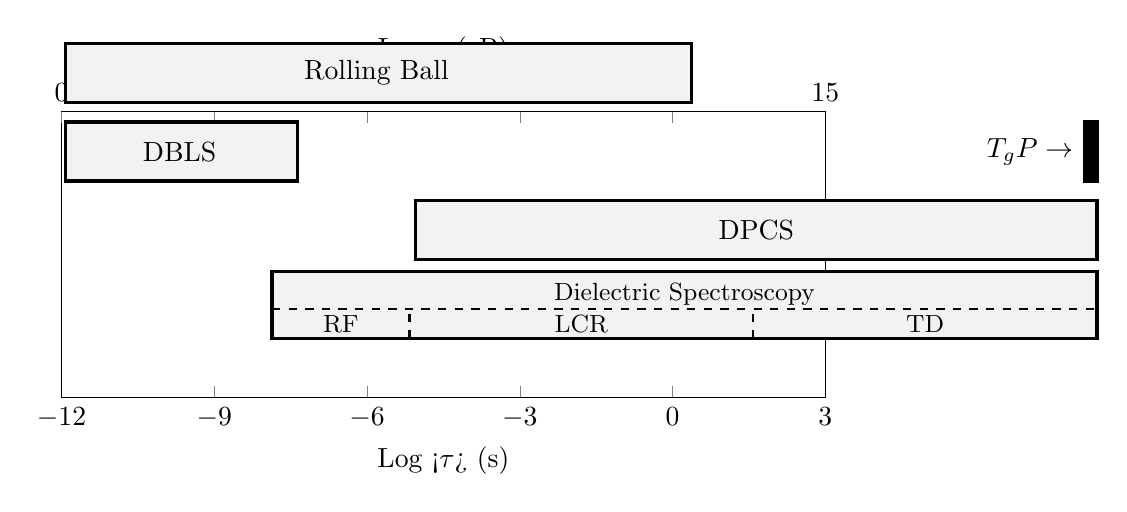
\begin{tikzpicture} 
		
		\begin{axis}[
			width=0.8\textwidth,
			height=0.3\textwidth,
			xlabel={Log <$\tau$> (s)},
			scale only axis,
			xmin=-12,xmax=3,
			xtick distance = 3,
			ymin=0,ymax=1,
			ytick=\empty,
			axis y line*=left,
			axis x line*=bottom]
			\addplot[]{-10}; %Just here to force the axis to print
		\end{axis}
		
		\begin{axis}[
			width=0.8\textwidth,
			height=0.3\textwidth,
			scale only axis,
			xmin=0,xmax=15,xtick={0,3,6,9,12,15},
			ymin=0,ymax=1,
			xtick distance = 5,
			ytick=\empty,
			domain=0:15,
			axis y line*=right,
			axis x line*=top,
			xlabel={Log $\eta$ (cP)}]
			\addplot[]{-10}; %Just here to force the axis to print
		\end{axis}
		
		%Box Representation of Rolling Ball
		\filldraw[black,fill=black!5, very thick] (0.055,3.75) rectangle (8,4.5);
		
		%Box Representation of DBLS
		\filldraw[black,fill=black!5, very thick] (0.055,2.75) rectangle (3,3.5);
		
		%Box Representation of DPCS
		\filldraw[black,fill=black!5, very thick] (4.5,1.75) rectangle (13.15,2.5);
		
		%Box Representation of DS
		\filldraw[black,fill=black!5, very thick] (2.674,0.75) rectangle (13.15,1.6);
		
		%Internal dashed divisions for DS
		\draw[dashed, thick] (2.674,1.125) -- (13.15,1.125);    %horizontal divider
		\draw[dashed, thick] (4.420,0.75) -- (4.420,1.125);     %RF | LCR at log tau = -7
		\draw[dashed, thick] (8.785,0.75) -- (8.785,1.125);     %LCR | TD at log tau = -2
		
		%Box Representation of TgP
		\filldraw[black,fill=black!100, very thick] (13,2.75) rectangle (13.15,3.5);
		
		\node at (12.3,3.125) {\tgp $\rightarrow$};
		\node at (4,4.125) {Rolling Ball};
		\node at (1.5,3.125) {DBLS};
		\node at (8.825,2.125) {DPCS};
		
		%DS labels
		\node[font=\small] at (7.912,1.3125) {Dielectric Spectroscopy};
		\node[font=\small] at (3.547,0.9375) {RF};
		\node[font=\small] at (6.6025,0.9375) {LCR};
		\node[font=\small] at (10.9675,0.9375) {TD};
		
	\end{tikzpicture}
	\caption{Accessible dynamic ranges for various probes of viscosity $\eta$ and structural relaxation time $\tau_\alpha$. Rolling Ball: rolling-ball viscometry (probe of $\eta$); DBLS: depolarized Brillouin light scattering; DPCS: depolarized photon correlation spectroscopy; DS: dielectric loss spectroscopy, shown as a composite of experimental regimes (dashed divisions): radio-frequency (RF), impedance/LCR, and time-domain (TD) measurements; \tgp: technique described in \sect\nolinebreak \ref{sec:IGPintro}.}
	\label{figure:Probes}
\end{figure}

The experimental probes referenced or implemented in this work are summarized in \fig \nolinebreak \ref{figure:Probes}. These include DPCS, DBLS, rolling ball viscometry, \tgp analysis, and DS. The physical mechanism behind each of these probes will be described briefly below as well as their dynamic windows and other limitations to their applicability pertinent to this work.  These descriptions will be kept intentionally brief as an entire dissertation could easily be written on any one of these probes alone, and indeed, \chap\nolinebreak \ref{chap:Glycerol} is in effect a reanalysis of one such dissertation outlining a means of extending a previously existing probe, rolling ball viscometry, into a diamond anvil cell allowing for viscosity measurements at higher pressures.\cite{CookThesis}  Following this, \chap\nolinebreak \ref{chap:PCS} will provide a similar extension, this time of photon correlation spectroscopy, into the diamond anvil cell.  Significantly more detail regarding these specific probes will be provided in their respective chapters.

\subsection{Depolarized Brillouin Light Scattering (DBLS)}
Electromagnetic interactions with matter lie at the heart of most experimental probes of structure and dynamics. Notable exceptions include ultrasonic techniques and neutron scattering, which rely on mechanical or nuclear interactions rather than electromagnetic coupling. Nevertheless, even neutron scattering possesses an electromagnetic aspect: the neutron’s appreciable magnetic moment renders it uniquely sensitive to ordered magnetic structures, such as spin fluctuations in superconducting materials \cite{Zaliznyak}. 

Light scattering methods probe how condensed matter responds to incident electromagnetic radiation, giving rise to a scattered field that carries information about the structure and dynamics of the bulk material. A generalized schematic for a light scattering experiment is shown in \fig \nolinebreak \ref{figure:SimpleDLS}. Polarized monochromatic laser light is collimated or focused through a sample volume, and a fraction of this light is scattered, collected, and directed onto a suitable spectral analyzer.

In the experiments presented in this dissertation, an intracavity etalon was employed to ensure single-mode laser operation with a spectral width of approximately $10~\si{\mega\hertz}$, as required for high-resolution Brillouin measurements. It is worth noting that other light scattering techniques, such as Raman scattering, commonly utilize multi-mode lasers with linewidths on the order of $\sim\si{\giga\hertz}$—still only about one part in $10^6$ of the optical carrier frequency. The scattered light in this work is analyzed using either a triple-pass tandem Fabry-P\'erot interferometer (DBLS) or a photon correlation spectrometer (DPCS).


\begin{figure}[!htbp]
	\centering
	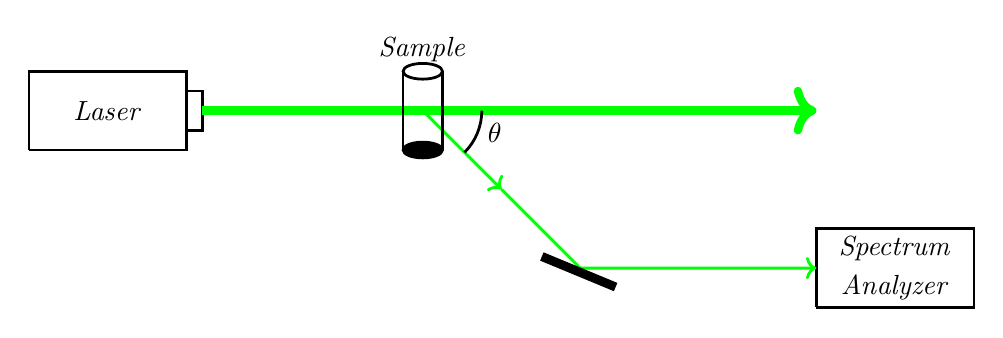
\begin{tikzpicture}
	%Laser
	\draw[line width=1pt] (0,0)--(2,0)--(2,1)--(0,1)--(0,0);
	\draw[line width=1pt] (2,.25)--(2.2,.25)--(2.2,.75)--(2,.75);
	\node[] at (1,.5) () {\textit{Laser}};
	
	%PMT
	\draw[line width=1pt] (10,-2)--(12,-2)--(12,-1)--(10,-1)--(10,-2);
	\node[] at (11,-1.25) () {\textit{Spectrum}};
	\node[] at (11,-1.75) () {\textit{Analyzer}};
	
	%Beams
	\draw[line width=3pt,color=green,->] (2.2,.5)--(10,.5);
	\draw[line width=1pt,color=green,->] (5,.5)--(6,-.5);
	\draw[line width=1pt,color=green,->] (6,-.5)--(7,-1.5)--(10,-1.5);
	\draw[line width=1pt] (5.75,.5) arc (0:-45:.75) node[midway,anchor=west] {$\theta$};
	
	%splitters
	\node[] at (7,-1.5) (c) {};
	\draw[rotate around={-22.5:(c)},fill=black] (7.5,-1.5) rectangle (6.5,-1.6);
	
	%Scatter Volume
	\node[anchor=south] at (5,1) () {\textit{Sample}};
	\node[] at (5,.5) (d) {}; %scatter volume center
	\draw[line width=1pt,fill=black] (5,0) ellipse (.25 and .1);
	\draw[line width=1pt] (5,1) ellipse (.25 and .1);
	\draw[line width=1pt] (5.25,0)--(5.25,1);
	\draw[line width=1pt] (4.75,0)--(4.75,1);
	
	\end{tikzpicture}
	\caption{A simple forward scattering DBLS experimental design in which light from a monochromatic source, such as a single mode locked AR\textsuperscript{+} laser, is scattered from a sample and collected at a known angle.  The collected light is then directed into a spectrum analyzer, such as a triple pass tandem Fabry-P\'erot interferometer.}\label{figure:SimpleDLS}
\end{figure}

A light source with exceedingly narrow spectral width is necessary for DBLS, as this probe resolves very small frequency shifts in the scattered light arising from dynamic processes within the sample. These processes will be described in more detail in \sect \nolinebreak \ref{sec:TheScatteredField} and \nolinebreak \ref{sec:SpectrumOfSimpleFluid}; for now, it suffices to note that light is scattered whenever there is a local temporal or spatial variation in the dielectric susceptibility of the medium. Such variations may arise from density fluctuations, induced dipoles, or orientational dynamics—anything that alters how the charges within the material respond to an applied electromagnetic field. If the susceptibility variation is purely spatial and static—for example, in a material with frozen-in density inhomogeneities—the scattered field retains the frequency of the incident beam, giving rise to elastic (Rayleigh) scattering. In fluids, however, density fluctuations are inherently time dependent. Any temporal modulation of the dielectric susceptibility must therefore produce a corresponding distribution of frequencies in the scattered field. Even crystalline solids exhibit such time-dependent fluctuations due to lattice vibrations. Longitudinal and transverse acoustic modes, as well as higher-frequency optical phonons, appear as frequency-shifted features in the scattered spectrum.

Depolarized Brillouin Light Scattering (DBLS), as implemented in this work, refers to the spectral analysis of depolarized scattered light using a high-resolution Fabry-P\'erot interferometer. Brillouin scattering arises from the interaction of light with thermally excited acoustic modes in the material—long-wavelength density fluctuations corresponding to small wavevector phonons in the GHz frequency regime. This distinguishes Brillouin scattering from Raman spectroscopy, which probes optical phonons or intramolecular vibrational modes at much higher (THz) frequencies and whose larger energy shifts are typically resolved using grating-based spectrometers.

In glass-forming liquids, the depolarized Brillouin spectrum contains not only acoustic sidebands but also a central quasielastic component. It is this central quasielastic feature, arising from time-dependent fluctuations in the anisotropic part of the dielectric susceptibility, that is of primary interest in the present work. This spectral component reflects structural relaxation processes within the bulk material and provides a direct probe of the $\alpha$-relaxation over a dynamic window approximately bounded by 
\[
10^{-12}\;\si{\second} \lesssim \tau_\alpha \lesssim 10^{-9}\;\si{\second},
\]
as shown in \fig \nolinebreak \ref{figure:Probes}.

While analysis of the linewidths of longitudinal acoustic (LA) Brillouin modes can provide access to viscoelastic damping and relaxation phenomena over a broader dynamic range \cite{Heiman}, such approaches probe relaxation indirectly through mechanical response functions. In contrast, the DBLS measurements discussed here focus specifically on the quasielastic depolarized spectrum as a more direct probe of structural $\alpha$-relaxation.

It is important to distinguish this spectrally resolved DBLS method from photon correlation spectroscopy (DPCS), which also probes $\alpha$-relaxation but does so through analysis of temporal fluctuations in scattered intensity rather than through frequency-domain spectral analysis. The two techniques therefore access distinct dynamic windows and rely on fundamentally different measurement formalisms.

\subsection{Depolarized Photon Correlation Spectroscopy (DPCS)} \label{sec:PCSintro}

Depolarized photon correlation spectroscopy (DPCS) is a light scattering technique, similar to DBLS described above, yet performed in the time domain. Both methods provide access to the $\alpha$-structural relaxation dynamics within a glass-forming liquid, however, they cover vastly different dynamic ranges. Whereas DBLS lends itself to probing very fast relaxations, on the order of tens to thousands of picoseconds, DPCS is generally applicable in the slow to intermediate dynamic regime, probing characteristic relaxation times ranging from tens of nanoseconds to thousands of seconds. A typical experimental setup for DPCS is shown in \fig \nolinebreak \ref{figure:SimpleDLS} \textemdash differing from DBLS only in the form of analyzer implemented. In fact, data taken for both DBLS and DPCS, analyzed in \chap \nolinebreak \ref{chap:PCS}, were all acquired on a single experimental setup in which a flip mirror allowed the collected scattered light from a sample to be directed either into a tandem triple-pass Fabry–Perot interferometer for frequency analysis or, alternatively, into a digital autocorrelator for temporal analysis.

There are two general experimental domains relevant to PCS\textemdash heterodyne and homodyne autocorrelation. It is important to define these terms here as there is some discrepancy within the literature regarding their use.  For the purposes of this work, homodyne PCS involves temporal correlation analysis of light scattered from a sample, where great care is taken to ensure that the detected signal arises solely from spontaneous density fluctuations within the material. Particular attention is given to minimizing parasitic elastic scattering and specular reflections from dust, cell windows, culets, or table surfaces, which could act as a coherent local oscillator and introduce heterodyne contributions to the measured correlation function.  The intensity of this scattered light will fluctuate as a result of any temporal dependency associated with these dynamic processes.  As such, this experimental arrangement is often referred to as ``self-beating,'' a designation that only becomes meaningful when contrasted with the alternative PCS configuration\textemdash heterodyne detection.

In a heterodyne experimental arrangement, such as is represented in \fig \nolinebreak \ref{figure:simpleHeterodyne}, a fraction of the source laser is split off before it is passed through the scattering sample and then re-mixed before being directed onto the detector for autocorrelation. In this arrangement, the fluctuations in detected intensity do not arise from the total number of scattering events, but rather from a shift in phase between light arising from scattering events and that of the local oscillator\textemdash a portion of the laser being mixed in providing a phase reference for the scattered light to beat against.  Below is shown one possible heterodyne experimental arrangement.  It is also common simply to collect light from the sample such that the specular reflection from the container can itself provide a local oscillator.  All that is required to operate within a heterodyne regime is that the local oscillator intensity be significantly greater than that of the light scattered from the sample.   Conversely, if one wishes to operate in a homodyne regime, one must ensure that any specular reflections or contributions from static scattering are negligible compared to the light scattered by the dynamic processes of interest within the sample. This often requires significant spatial filtering as well as exceedingly pure samples and clean experimental environments.

\begin{figure}[!htbp]
	\centering
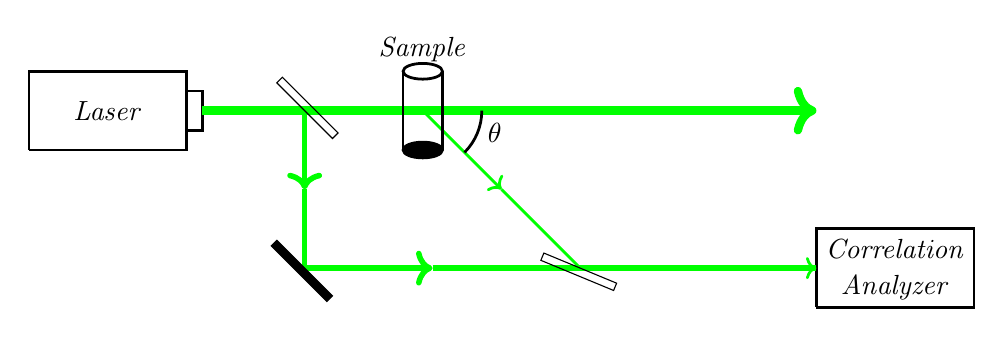
\begin{tikzpicture}
	%Laser
	\draw[line width=1pt] (0,0)--(2,0)--(2,1)--(0,1)--(0,0);
	\draw[line width=1pt] (2,.25)--(2.2,.25)--(2.2,.75)--(2,.75);
	\node[] at (1,.5) () {\textit{Laser}};
	
	%PMT
	\draw[line width=1pt] (10,-2)--(12,-2)--(12,-1)--(10,-1)--(10,-2);
	\node[] at (11,-1.25) () {\textit{Correlation}};
	\node[] at (11,-1.75) () {\textit{Analyzer}};
	
	%Beams
	\draw[line width=3pt,color=green,->] (2.2,.5)--(10,.5);
	\draw[line width=1pt,color=green,->] (5,.5)--(6,-.5);
	\draw[line width=1pt,color=green,->] (6,-.5)--(7,-1.5)--(10,-1.5);
	\draw[line width=1pt] (5.75,.5) arc (0:-45:.75) node[midway,anchor=west] {$\theta$};
	\draw[line width=2pt,color=green,->] (3.5,.5)--(3.5,-.5);
	\draw[line width=2pt,color=green] (3.5,-.5)--(3.5,-1.5);
	\draw[line width=2pt,color=green,->] (3.5,-1.5)--(5.125,-1.5);
	\draw[line width=2pt,color=green] (5.125,-1.5)--(10,-1.5);
	
	%splitters
	\node[] at (3.5,.5) (a) {}; %splitter center
	\draw[rotate around={-45:(a)}] (3,.5) rectangle (4,.6);
	\node[] at (3.5,-1.5) (b) {}; %splitter center
	\draw[rotate around={-45:(b)},fill=black] (3,-1.5) rectangle (4,-1.6);
	\node[] at (7,-1.5) (c) {};
	\draw[rotate around={-22.5:(c)}] (7.5,-1.5) rectangle (6.5,-1.6);
	
	%Scatter Volume
	\node[anchor=south] at (5,1) () {\textit{Sample}};
	\node[] at (5,.5) (d) {}; %scatter volume center
	\draw[line width=1pt,fill=black] (5,0) ellipse (.25 and .1);
	\draw[line width=1pt] (5,1) ellipse (.25 and .1);
	\draw[line width=1pt] (5.25,0)--(5.25,1);
	\draw[line width=1pt] (4.75,0)--(4.75,1);

\end{tikzpicture}
\caption{Heterodyne experimental arrangement for PCS.  A local oscillator is mixed with the scattered signal before being redirected onto the photomultiplier or other detector.}
\label{figure:simpleHeterodyne}
\end{figure}

In both experimental arrangements the intensity fluctuations at the detector are due to the same fluctuations in the local density or dielectric constant within the scattering volume in the sample, however, the two methods measure different correlation functions of these fluctuations.  Thus, proper analysis of resulting data requires that one be firmly within one or the other experimental domain.  It is generally very undesirable to be within an intermediate homodyne/heterodyne scenario.  If a homodyne experiment is desired one must often take great care to assure that only light arising from the scattering events of interest are collected.  Dust and contaminates, both within the sample and on the sample container, or even undesired specular reflections may give rise to undesired heterodyne components which may make proper data analysis challenging or even impossible.  These concerns are not always easily mitigated, and great care is required to identify the regime in which one is operating, as will be discussed in \sect \nolinebreak \ref{sec:HomoHeto}, where a method for extending PCS to high-pressure is described in detail.


\subsection{Rolling Ball Viscometry} \label{sec:rolling_ball}

Rolling or falling Ball viscometry provides a means of direct mechanical measurement of viscosity.  Many different types of high pressure vicometers and their range of application are described in more detail by Cook, Herbst, and King\cite{Cook}.  These methods generally implement a spherical ball as it moves through a viscous fluid under the influence of gravity or other forces.  Placing this ball within a diamond anvil cell allows access to very high pressures however the viscosities that can be measured are obviously limited to those low enough for a macroscopic ball to progress through the material during the course of a reasonable experimental timescale.  In practice this means that rolling and falling ball viscometry in a diamond anvil cell is limited to approximately $10^7$ cP\textemdash eight orders of magnitude away from the glass transition.  In the work previously cited, Cook \etal managed to extend this viscosity range an additional two and a half orders of magnitude, up to approximately $10^{9}$ cP, \via placing the diamond anvil cell viscometer onto a centrifuge which greatly increases the g-forces driving the ball through the fluid\cite{Cook}.  However this still limits the probe to a viscosity range many orders of magnitude away from the glass transition.

Though this probe cannot provide measurements in the vicinity of the glass transition it does, as shown in \fig \nolinebreak \ref{figure:Probes}, provide access to a very large dynamic range of viscosities\textemdash up to nine orders of magnitude.  There are some experimental concerns even within its range of application.  Specifically, rolling ball viscometry relies on a correction, or ``wall factor,'' that accounts for dissipative losses as the ball rolls down the diamond surface within the cell.  This correction factor is assumed to be constant as experimental variables such as pressure and temperature are changed.  It is also generally assumed that the probe ball is rolling down the diamond cutlet without slipping.  It is very difficult, if not impossible, to directly verify the degree to which these assumptions hold over the entire range of experimental parameters.  However this work will show that data for the glass former glycerol obtained by Cook \etal \via rolling ball viscometry appears to be reasonably consistent over its applicable range with data taken \via other probes and non-related methods.

\subsection{\tgp} \label{sec:IGPintro}

The \tgp process is a very straight forward means of measuring the isochronal curve of the glass transition temperature $T_{g}$ as a function of Pressure.  A liquid is loaded into a diamond anvil cell and brought to a temperature and pressure such that it is well within the solid glass phase.  It has been found advantageous to pre-indent the gasket, which hardens it, thus making higher pressures more achievable.  Two or more rubies are arranged throughout the sample as shown in the far left DAC in \fig \nolinebreak \ref{figure:tgpgrade}.  A pressure gradient is then applied to the DAC \via asymmetric application of force as indicated by the dashed Isobaric Lines. 
\begin{figure}[!htbp]
	\centering
	\includegraphics[width=0.8\textwidth]{gradient.jpg}
	\caption{Pressure gradients established within a diamond anvil cell decrease as temperature increases and the system approaches the glass transition from the glassy state, ultimately attaining hydrostatic conditions. This figure is reproduced from Ref.~\cite{RansomPRL}.}
	\label{figure:tgpgrade}
\end{figure}
Temperature is then increased incrementally, typically in 5 to 10 degree steps initially and then smaller steps as the glass transition is approached as evident \via the pressure gradients giving way to hydrostatic conditions above $T_{g}$.  At each temperature, pressure is measured from a consistent  location on each ruby to again check for pressure gradients.  Temperature is then increased to a new set point and a small set time is allowed for the sample to reestablish thermal equilibrium.  A means of determining the approximate temperature at which the gradients dissolve and the material transitions into a liquid have been developed previously and described in Ref. \nolinebreak \cite{RansomPRL,Ransom}.  The values obtained for the glass transition temperatures as a function of pressure are fit to an Andersson-Andersson equation \cite{Andersson} provided along with data for glycerol and cumene in \app \nolinebreak  \ref{app:GlycerolIGP} and \nolinebreak \ref{app:CumeneIGP} respectively. The automation of this process will increase its efficacy in the future and may even allow it to provide more than a single isochronal curve near and around the glass transition.  


\subsection{Dielectric Loss Spectrometry} \label{sec:FRAintro}

Frequency Response Analysis encompasses various methods capable of measuring molecular dynamics over an exceptionally broad dynamic range. Among these, Dielectric Spectroscopy (DS) is particularly important and will be extensively discussed in this dissertation. DS takes advantage of molecular dipole moments, which either inherently exist or are induced by an applied oscillating electric field.

As molecular orientations within the glass-forming liquid respond to an applied external field, dielectric spectroscopy (DS) measures both the real and imaginary components of the complex dielectric constant. When the frequency of the applied field is systematically swept—from fractions of a hertz to several gigahertz—the imaginary component plotted as a function of frequency forms the dielectric loss spectrum. Peaks in this loss spectrum correspond directly to molecular relaxation processes occurring within the sample. 

Alternatively, DS measurements may be performed at fixed frequency while varying temperature or pressure, with both components of the dielectric response recorded as functions of $T$ or $P$. In either protocol, the rate at which frequency, temperature, or pressure is varied plays an important role in determining the apparent relaxation behavior. By monitoring how the positions of loss maxima evolve under controlled thermodynamic conditions, researchers gain access to molecular dynamics such as the structural relaxation time ($\tau_{\alpha}$), as well as faster secondary processes, commonly referred to as $\beta$-relaxations.

However, dielectric spectroscopy provides considerably more information than merely the characteristic structural relaxation times inferred from dielectric loss peaks. Both the real and imaginary components of the complex dielectric constant contain dynamical information. When analyzed together, these components may be represented in the complex plane to form characteristic Cole--Cole or Cole--Davidson plots \cite{Davidson}. Such representations facilitate visualization of relaxation behavior and, when combined with appropriate empirical response functions, enable extraction of additional parameters. Among these is the stretching exponent $\beta$, which reflects the breadth of the underlying distribution of relaxation times and the degree of dynamical heterogeneity within the glass-forming liquid. Representative examples illustrating both Debye-like and stretched-exponential behavior are presented in \chap \nolinebreak \ref{chap:Glycerol} (see, for example, \fig \nolinebreak \ref{figure:glcyerolcolecole}).

Given its capability to provide a wide array of parameters and its extensive dynamic range, dielectric spectroscopy is one of the most powerful and widely implemented experimental methods in glass transition research. Indeed, due to its comprehensive coverage of both structural and secondary relaxations, DS serves as an indispensable tool for studying the complex molecular dynamics of glass-forming liquids, a role this dissertation will explore further.

\chapter{Supporting Theory}
\label{chap:theory}

This chapter introduces key concepts and theoretical tools relevant to the study of glass-forming liquids. In particular, important quantities such as fragility will be formally defined, with a more detailed discussion deferred to \sect \ref{sec:Fragility}. In addition, a scaled definition of fragility will be introduced and developed in that context.

The remainder of the chapter focuses on the theoretical framework underlying the experimental techniques used in this work. A derivation of the scattered radiation field is presented, establishing the connection between the measured signal and the dynamics of the liquid under study. The spectral structure of light scattered from a simple fluid is then discussed, along with its transformation into the time domain through intensity autocorrelation. Finally, mathematical models used to describe these scattered fields and extract thermodynamic parameters of interest are introduced.


\section{Fragility} \label{sec:Fragility}

Fragility is a useful parameter for describing the dynamic behavior of a glass-forming liquid as the glass transition is approached. Early work by Angell~\cite{Angell1985} introduced the concept through a classification of liquids as ``strong'' or ``fragile,'' based on the degree to which their viscosity or structural relaxation dynamics deviate from Arrhenius behavior upon cooling. 

\graphicspath{{Chapters/Methodology/Figures/}}

\begin{figure}[!htbp]
	\centering
	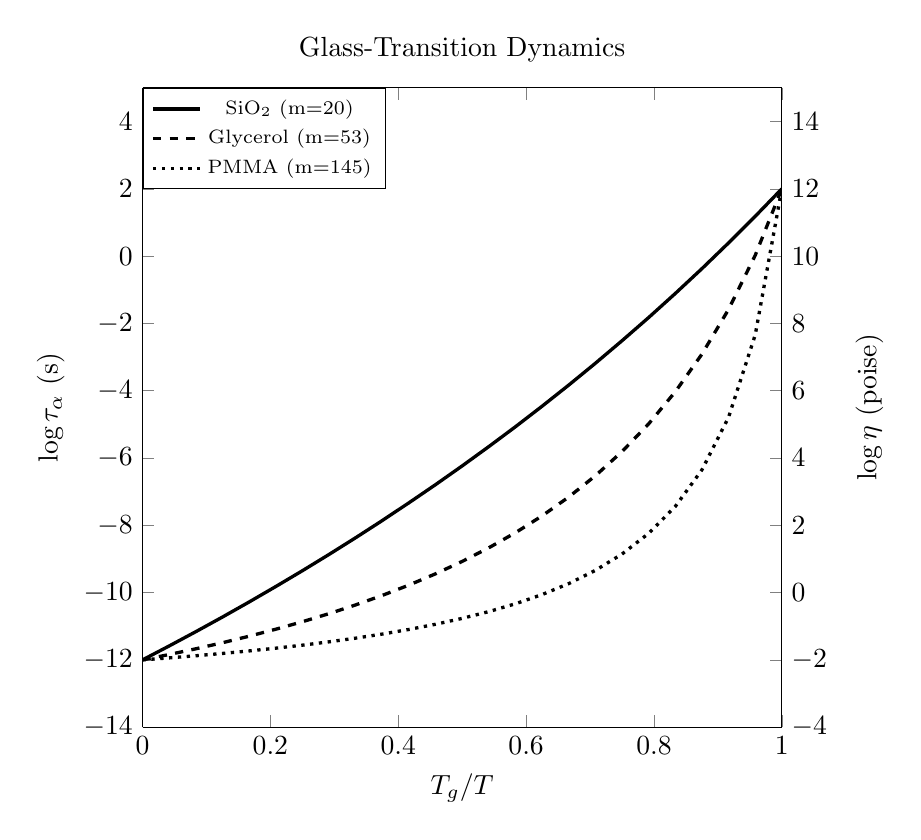
\begin{tikzpicture}[>=latex]
		\begin{axis}[
			width=0.8\textwidth,
			height=0.8\textwidth,
			xmin=0,xmax=1,
			ymin=-4,ymax=15,
			xtick=\empty,
			domain=0:15,
			axis y line*=right,
			axis x line*=none,
			y label style={at={(axis description cs:1.1,.5)},anchor=north},
			ylabel={$\log\eta$ (poise)},
			]
		\end{axis}
		
		\begin{axis}[
			legend style={at={(0,1)},anchor=north west},
			title={Glass-Transition Dynamics},
			width=.8\textwidth,
			height=.8\textwidth,
			axis y line*=left,
			xmin=0,xmax=1,
			ymin=-14,ymax=5,
			ylabel={$\log\tau_\alpha$ (s)},
			xlabel={$T_g/T$},
			]
			\addplot expression[domain=0:1,black, very thick, solid, mark=none]{
				-44.6666666667 - 108.8888888889/(x - 3.3333333333)
			}; 
			\addlegendentry{{\scriptsize SiO\textsubscript{2} (m=20)}}
			
			\addplot expression[domain=0:1,black, very thick, dashed,mark=none]{
				-17.0256410256 - 6.8297172913/(x - 1.3589743590)
			}; 
			\addlegendentry{{\scriptsize Glycerol (m=53)}}
			
			\addplot expression[domain=0:1,black, very thick, dotted,mark=none]{
				-13.4961832061 - 1.6560806480/(x - 1.1068702290)
			};
			\addlegendentry{{\scriptsize PMMA (m=145)}}
		\end{axis}
	\end{tikzpicture}
	
	\caption{Representative Angell plots illustrating the fragility of three glass-forming systems. These curves are idealized constructions chosen to reproduce the accepted ambient-pressure fragility values and are not intended to represent experimental data. Both the glass-transition and high-temperature limits are imposed to define a common dynamic range. In this representation, each system is scaled by its respective glass transition temperature $T_g$, allowing direct comparison on a common framework. Strong (Arrhenius) liquids display approximately linear behavior, whereas fragile liquids exhibit pronounced super-Arrhenius curvature as $T_g$ is approached.}
	\label{figure:AngellPlot}
\end{figure}

\noindent The Angell plot, shown in \fig\nolinebreak\ref{figure:AngellPlot}, provides a compact and intuitive representation of glass-forming dynamics. In this representation, the logarithm of either the viscosity, $\eta$, or the structural relaxation time, $\tau_\alpha$, is plotted as a function of inverse temperature normalized by the glass-transition temperature, $T_g/T$. These quantities are related through the Maxwell relation,

\begin{equation}
	\eta = G_\infty \tau_\alpha,
\end{equation}

\noindent where $G_\infty$ is the high-frequency (instantaneous) shear modulus. This relation allows either viscosity or structural relaxation time to serve as a measure of the underlying dynamics.

The horizontal axis of a classic Angell plot progresses from high temperature on the left to the glass transition at $T_g/T = 1$ on the right. This representation highlights the enormous dynamic range spanned by glass-forming liquids, with viscosity or relaxation time changing by many orders of magnitude as the system is supercooled toward $T_g$. Because each system is normalized by its own glass-transition temperature, Angell plots enable direct comparison across materials with widely differing intermolecular interactions and absolute timescales.

If one defines the high-temperature asymptotic limit as the regime in which the average thermal energy of any given molecule greatly exceeds the characteristic intermolecular interaction energies, then intermolecular constraints cease to dominate the structural dynamics of the liquid. In this regime, the system approaches behavior characteristic of weakly interacting particles, and relaxation is governed primarily by intrinsic molecular parameters rather than cooperative rearrangements. Although the liquid phase itself will ultimately lose thermodynamic stability at sufficiently high temperature, within the accessible liquid domain the relaxation dynamics progressively lose sensitivity to collective structural constraints.

As intermolecular barriers become energetically insignificant relative to $k_{B}T$, the system samples the potential energy landscape with minimal constraint. Structural relaxation is therefore controlled primarily by internal molecular properties such as moments of inertia and local conformational flexibility. Most small organic molecules span only a few angstroms, and even larger macromolecules exhibit local flexibility on comparable length scales. Consequently, the characteristic microscopic times associated with molecular motion tend to fall within similar ranges across many liquids. It is therefore not surprising that, under a given isobaric condition, liquids exhibit high-temperature asymptotic relaxation times $\tau_{\alpha}$ confined to a relatively narrow window, typically from hundreds of femtoseconds to a few picoseconds.

\fig\nolinebreak\ref{figure:AngellPlot} shows the Angell plot for three distinct glass-forming systems. Molten silicon dioxide serves as a classic example of an Arrhenius, or what Angell termed a ``strong'' liquid. Glycerol provides an example of a liquid intermediate in fragility, while the polymer PMMA exhibits highly super-Arrhenius behavior characteristic of a fragile system. Although these materials differ significantly in their intermolecular bonding---from network-forming covalent structures in \ce{SiO2}, to hydrogen bonding in glycerol, to van der Waals-dominated interactions in simple molecular liquids such as cumene, and to polymeric systems such as PMMA---fragility itself does not necessarily reflect bond strength. Rather, it characterizes how strongly the relaxation dynamics depend on temperature as the glass transition is approached.

Common network-forming liquids, such as silicates, exhibit nearly linear behavior on an Angell plot and are referred to as ``strong'' glass formers. This corresponds to an approximately Arrhenius temperature dependence of the viscosity or structural relaxation time. In contrast, many glass-forming liquids exhibit pronounced curvature in this representation, reflecting strong deviations from Arrhenius behavior. These systems are referred to as ``fragile'' glass formers.

Fragility therefore provides a quantitative measure of the degree to which a liquid’s dynamics deviate from Arrhenius behavior as the glass transition is approached. The Angell plot provides a compact means to compare the dynamics of different glass-forming systems on a single graph while simultaneously visualizing their fragilities. As defined in \eqn\nolinebreak\ref{eqn:fragility}, fragility is geometrically represented as the slope of the Angell plot at $T_g/T = 1$, \ie, as the system approaches the glass transition from the liquid state. Thus, the relative fragilities of different liquids---or of a single liquid under varying pressure---can be determined at a glance.

\begin{equation}
	m=\left ( \frac{\partial \log_{10}\eta}{\partial \left ( T_g/T \right )} \right )_{T=T_g}
	\label{eqn:fragility}
\end{equation}

\noindent This definition is inherently isobaric, as it is constructed from temperature-dependent measurements performed at fixed pressure. While Angell’s original definition emphasizes temperature-dependent behavior, comparable dynamical changes occur under compression, setting the stage for the pressure-dependent investigations presented in this work.

Because the horizontal axis of a proper Angell plot progresses from zero to one as $T_g/T$ increases, and many liquids exhibit a comparable high-temperature asymptotic viscosity on the order of $10^{-3}$--$10^{-4}$~p, the minimum fragility attainable under the conventional definition corresponds to the slope of a straight line connecting this asymptotic viscosity to that at which the glass transition is defined to occur. Taking $\eta_g \equiv 10^{13}$~p, a nearly Arrhenius liquid therefore exhibits a fragility on the order of $m \approx 16$.

Although the conventional fragility is defined as the slope of the Angell plot at $T_g$, the choice of $T_g$ itself---fixed by selecting a particular dynamical value---implicitly embeds the dynamic range into the definition. As a result, even a perfectly Arrhenius liquid does not assume a value of unity. It is therefore more natural to rescale the ordinate of the Angell representation and redefine fragility accordingly, such that an Arrhenius liquid serves as the reference case with scaled fragility equal to one.

\begin{equation}
	m^*=\frac{1}{\log_{10}\left( \frac{\eta_g}{ \eta_\infty}\right )} \left ( \frac{\partial \log_{10}\left( \frac{\eta}{ \eta_\infty}\right )}{\partial \left ( T_g/T \right )} \right )_{T=T_g}
	\label{eqn:scaledfragility}
\end{equation}

In practice, this redefinition merely rescales the classic Angell fragility by a constant normalization factor. It introduces no additional complexity into the analysis, yet it enforces well-defined high- and low-temperature limits in the Angell representation and removes ambiguity in interpretation: a purely Arrhenius system exhibits a scaled fragility of precisely $m^{\ast}=1$. By embedding the dynamic range explicitly within the definition, the scaled fragility also facilitates consistent comparison between viscosity data and structural relaxation measurements.

\begin{figure}[!htbp]
	\centering
	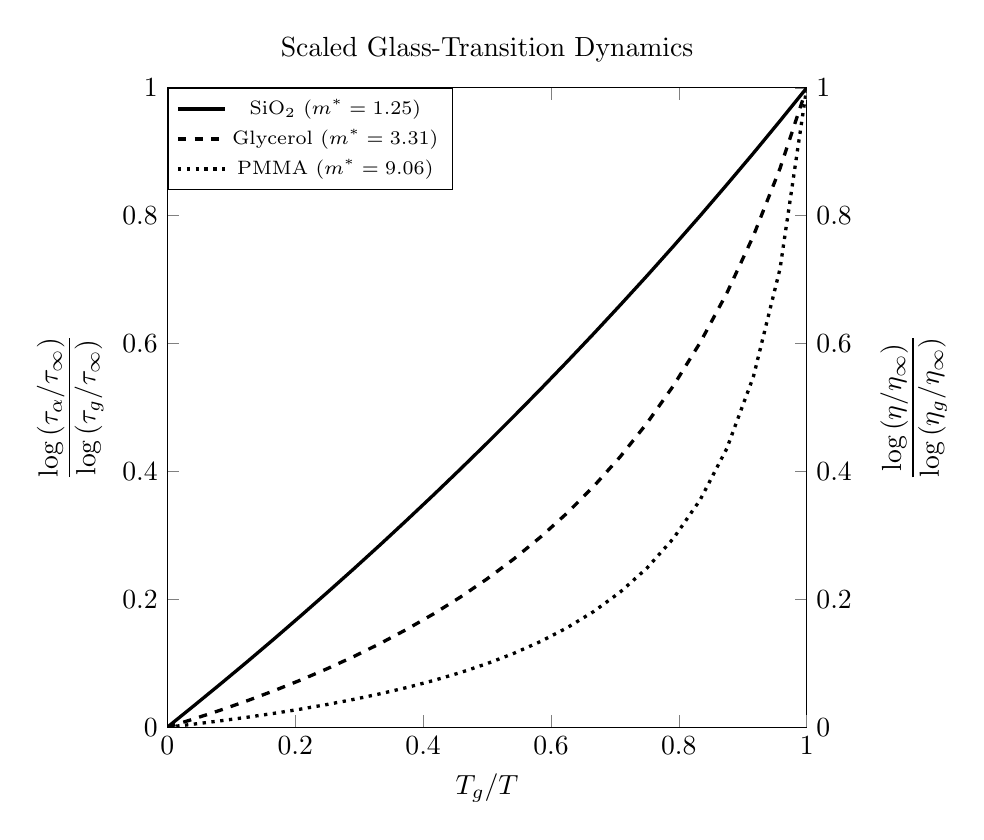
\begin{tikzpicture}[>=latex]
		\begin{axis}[
			width=0.8\textwidth,
			height=0.8\textwidth,
			xmin=0,xmax=1,
			ymin=0,ymax=1,
			xtick=\empty,
			axis y line*=right,
			axis x line*=none,
			y label style={at={(axis description cs:1.1,.5)},anchor=north},
			ylabel={$\displaystyle \frac{\log\left(\eta/\eta_\infty\right)}{\log\left(\eta_g/\eta_\infty\right)}$},
			]
		\end{axis}
		
		\begin{axis}[
			legend style={at={(0,1)},anchor=north west},
			title={Scaled Glass-Transition Dynamics},
			width=.8\textwidth,
			height=.8\textwidth,
			axis y line*=left,
			xmin=0,xmax=1,
			ymin=0,ymax=1,
			ylabel={$\displaystyle \frac{\log\left(\tau_\alpha/\tau_\infty\right)}{\log\left(\tau_g/\tau_\infty\right)}$},
			xlabel={$T_g/T$},
			]
			\addplot expression[domain=0:1,black, very thick, solid, mark=none]{
				log10(10^(-78-320/(x-5))/10^(-14))/16
			};
			\addlegendentry{{\scriptsize SiO\textsubscript{2} ($m^*=1.25$)}}
			
			\addplot expression[domain=0:1,black, very thick, dashed, mark=none]{
				log10(10^(-20.9189-9.91088/(x-1.43243))/10^(-14))/16
			};
			\addlegendentry{{\scriptsize Glycerol ($m^*=3.31$)}}
			
			\addplot expression[domain=0:1,black, very thick, dotted, mark=none]{
				log10(10^(-15.9845-2.23064/(x-1.12403))/10^(-14))/16
			};
			\addlegendentry{{\scriptsize PMMA ($m^*=9.06$)}}
		\end{axis}
	\end{tikzpicture}
	
	\caption{Scaled Angell plots for the same three liquids shown in \fig\nolinebreak\ref{figure:AngellPlot}, constrained at both the glass transition and in the high-temperature limit. In this representation, the dynamic range is normalized such that a purely Arrhenius liquid exhibits a scaled fragility of $m^{\ast}=1$.}
	\label{figure:ScaledAngellPlot}
\end{figure}

The scaled Angell plot shown in \fig\nolinebreak\ref{figure:ScaledAngellPlot} retains the same qualitative behavior as \fig\nolinebreak\ref{figure:AngellPlot}. In the classic Angell representation, the high-temperature asymptotic viscosities or relaxation times are not constrained to coincide, so the curves remain vertically offset at low $T_g/T$. By contrast, the scaled representation normalizes by the total dynamic range between the high-temperature asymptote and the glass-transition point, allowing direct comparison across systems with differing intrinsic viscosity spans. In this representation, both viscosity and structural relaxation data share a common dimensionless scale.

Importantly, many glass-forming liquids exhibit a similar limiting behavior at high temperatures, where relaxation dynamics approach a common Arrhenius-like regime. The scaled Angell representation leverages this convergence by explicitly normalizing both the high-temperature limit and the glass-transition point. In doing so, it provides a more rigorous and universal definition of fragility, wherein the minimum possible scaled fragility is, by construction, $m^* = 1$.

This work is certainly not the first to suggest an adaptation to fragility. Various alternative definitions and reinterpretations appear throughout the literature. However, the scaled fragility adopted here is particularly useful because it preserves the intuitive geometrical meaning of the Angell slope while removing the arbitrary offset imposed by the conventional dynamic range. This normalization removes ambiguity associated with differing experimental probes and absolute timescales, allowing deviations from Arrhenius behavior to be compared on an equal footing across materials.

One of the central aims of this work is to extend these concepts beyond ambient conditions and investigate how fragility evolves under compression. By incorporating pressure as an additional thermodynamic variable, it becomes possible to explore fragility not as a single scalar quantity, but as a property defined over a continuous thermodynamic surface.

\subsection{Arrhenius Systems} \label{sec:Arrhenius}

Arrhenius, or ``strong,'' glass-forming liquids are those whose primary structural relaxation exhibits an approximately temperature-independent activation energy as the glass transition is approached. In such systems, structural rearrangement occurs through thermally activated processes, with the probability of overcoming an energy barrier $\Delta E$ governed by Boltzmann statistics. Consequently, the relaxation time and viscosity follow an exponential dependence on inverse temperature,

\begin{equation}
	\tau_\alpha=\tau_\infty  \exp\left [ \frac{\Delta E}{k_{B}T} \right ]
	\label{eqn:arrhenius}
\end{equation}

\noindent where $\tau_\infty$ represents the high-temperature asymptotic relaxation time corresponding to the limit in which intermolecular constraints no longer significantly impede molecular motion.

A classic example is silicon dioxide (SiO\textsubscript{2}), which exhibits nearly linear behavior on an Angell plot, consistent with Arrhenius dynamics. Such systems approach the minimum fragility limit, typically $m \approx 15$--$16$ in the conventional definition, reflecting the fixed dynamic range embedded in the Angell representation. 

\subsection{Non-Arrhenius Systems}

Most glass-forming liquids do not exhibit purely Arrhenius behavior. Even systems typically classified as ``strong,'' such as SiO\textsubscript{2}, display some degree of curvature on an Angell plot, indicating deviations from a single, temperature-independent activation energy. In realistic systems, the presence of multiple relaxation pathways lead to a distribution of energy barriers, giving rise to non-Arrhenius dynamics.

Glass-forming liquids that exhibit pronounced deviations from Arrhenius behavior are referred to as ``fragile'' glass formers. In these systems, the effective activation energy governing structural relaxation becomes temperature dependent. At high temperature, the apparent activation energy is relatively small, but as the glass transition is approached, the effective barrier increases, leading to strongly super-Arrhenius behavior. A PMMA melt is a classic example of a fragile glass-forming liquid, while glycerol is typically considered to exhibit intermediate fragility.

The terminology ``strong'' and ``fragile,'' introduced by Angell, refers specifically to the temperature dependence of the relaxation dynamics and not to mechanical strength in the conventional sense. ``Strong'' liquids exhibit nearly Arrhenius behavior, indicating a relatively weak temperature dependence of the activation barrier, whereas ``fragile'' liquids display pronounced super-Arrhenius behavior, reflecting a rapidly increasing effective barrier as the glass transition is approached. These terms are therefore best understood as describing dynamical sensitivity to temperature rather than any intrinsic mechanical property of the material.

Fragility in such systems may also be pressure-dependent. Glycerol provides a notable example, as its fragility increases with increasing pressure, an effect attributed to the suppression of hydrogen bonding. This pressure dependence will be explored in detail in \chap\nolinebreak\ref{chap:Glycerol}.

The temperature dependence of non-Arrhenius dynamics is commonly described using the Vogel--Tammann--Fulcher (VTF) equation, first proposed by Tammann and Hesse in 1926, to describe the temperature dependence of viscosity in polar liquids \cite{Tammann}.  The modern form of this equation, most prevalent in the literature, is given by

\begin{equation}
	\centering
	\tau_\alpha=\tau_\infty  \exp\left [ \frac{DT_0}{T-T_0} \right ]
	\label{eqn:VTFintro}
\end{equation}

\noindent where $T_0$ is the extrapolated temperature at which the relaxation time diverges, often referred to as the zero-mobility temperature, and $D$ is a material-dependent parameter related to fragility. This form captures the rapid growth of relaxation times as the system approaches the glass transition from the liquid state.

\section{Dielectric Fluctuations and Light Scattering}
\label{sec:TheScatteredField}

Any time light travels through a transparent medium, electromagnetic fields couple with charges within the medium, inducing electronic moments. This interaction can be quite complicated, resulting in a scattered field that requires a multipole expansion to describe properly. However, in the limit where the wavelength of the incident field is large compared to the characteristic microscopic length scales within the medium, the electric dipole term generally dominates and the induced polarization may be treated in the quasi-static (long-wavelength) limit, where spatial variations of the field across a scattering region are negligible \cite[p.~572]{Jackson}. 

The general form of the scattered field, though technically a quantum effect, can be derived via classical electrodynamic theory and is well described in general terms by both Jackson and Landau–Lifshitz, while Berne and Pecora offer a more practical rendition of Landau’s derivation specifically in the context of dynamic light scattering\nolinebreak \cite{Landau,Jackson,Berne}. In all cases, an incident monochromatic plane wave is assumed to propagate through a scattering medium as depicted in \fig \nolinebreak \ref{figure:planescatter}.

An incident monochromatic plane wave, indicated by the vertical blue lines, propagates in the $+\hat{z}$ direction with wavevector
\begin{equation}
\vec{k}_{in} = \frac{2 n \pi}{\lambda_{in}},
\end{equation}
where $\lambda_{in}$ is the incident wavelength in vacuum and $n$ is the refractive index of the medium. Light scattered by the medium is collected at a scattering angle $\theta_S$ relative to the incident direction, as indicated by the dashed arrows, with outgoing wavevector

\begin{equation}
\vec{k}_{out} = \frac{2 n \pi}{\lambda_{out}}.
\end{equation}

Typical laser wavelengths used in light-scattering experiments are on the order of $\lambda_{in} \approx 500~\text{nm}$, corresponding to optical frequencies near $6\times10^{14}~\text{Hz}$. For a representative refractive index of $n \approx 1.4$, the magnitude of the incident wavevector is therefore
\begin{equation}
k_{in} \approx \frac{2(1.4)\pi}{500\times10^{-9}\,\text{m}} \approx 1.8\times10^{7}~\text{m}^{-1}.
\end{equation}

In inelastic Brillouin light scattering, the scattered light typically differs in frequency from the incident light by at most a few gigahertz, while in quasi-elastic photon correlation spectroscopy (PCS), the frequency shifts range from sub-hertz to megahertz. In either case, these shifts are negligible compared to the optical carrier frequency. It is therefore an excellent approximation to assume $\lambda_{out} \approx \lambda_{in}$, so that $|\vec{k}_{out}| \approx |\vec{k}_{in}| \equiv k$. Under this assumption, the scattering vector
\begin{equation}
\vec{q} = \vec{k}_{out} - \vec{k}_{in}
\end{equation}
\noindent has magnitude, via the law of cosines,
\begin{equation}
q = 2k \sin\left(\frac{\theta_S}{2}\right).
\end{equation}
\noindent This long-wavelength approximation, in which the incoming and outgoing wavelengths are effectively identical, constitutes one of the primary assumptions underlying the analysis that follows.

For typical scattering angles employed in Brillouin light-scattering experiments, $q$ is on the same order as $k_{in}$, and the frequencies of the Stokes and anti-Stokes Brillouin shifts are determined by the acoustic velocity $v$ of the medium according to
\begin{equation}
\nu = \frac{q v}{2\pi}.
\end{equation}

In PCS experiments on simple fluids, the relevant density fluctuations occur over spatial scales that are small compared to the wavelength, provided the system is not near a critical point where macroscopic critical fluctuations would dominate \cite{Stanley1971}. Although dynamic heterogeneities grow as the glass transition is approached, their characteristic length scales remain on the order of only a few molecular diameters (i.e., nanometers), far below optical wavelengths in typical glass-forming liquids~\cite{BerthierBiroli2011,Ediger2000}. In this limit, the electromagnetic field is effectively uniform across each microscopic scattering region, and all molecules within that region experience essentially the same local electric field. The total scattering volume in an experiment then consists of many such statistically independent regions, and the scattered light collected represents the coherent superposition of the fields radiated by each region. This physical picture of light scattering from thermodynamic density fluctuations was first articulated by Einstein in his early treatment of critical opalescence \cite{Einstein1910}.


\begin{figure}[!htbp]
	\centering
	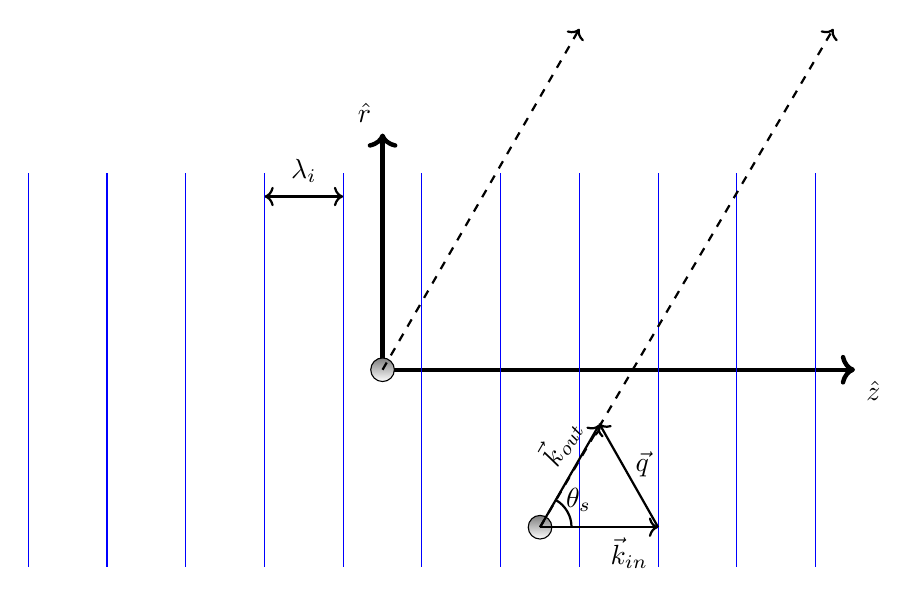
\begin{tikzpicture}
		%Z-Axis
		\draw[ultra thick,->] (0,0) -- (6,0) node[anchor=north west] {$\hat{z}$};
		\draw[ultra thick,->] (0,0) -- (0,3) node[anchor=south east] {$\hat{r}$};
		
		% Wavelength indicator (top left)
		\draw[<->, thick] (-1.5,2.2) -- (-0.5,2.2);
		\node[anchor=south] at (-1.0,2.25) {$\lambda_i$};
		
		
		\foreach \x in {-4,-3,-2,-1,0,1,2,3,4,5,6}
		\draw[thin, blue] (\x-.5,-2.5) -- (\x-.5,2.5);
		\draw[shade] (2,-2) circle (0.15cm);
		\draw[shade] (0,0) circle (0.15cm);
		
		%K Vectors
		\draw[thick,->]  (2,-2) -- (3.5,-2)  node[anchor=north east] {$\vec{k}_{in}$};
		\draw[thick,->] (2,-2) -- (2.75,-0.700961894) node[anchor=south east,rotate=60] {$\vec{k}_{out}$};
		\draw[thick,<-] (2.75,-0.68)--(3.5,-2); 
		\node[] at (3.3,-1.2) {$\vec{q}$};
		%arc for scatter vector
		\draw[thick] (2.4,-2) arc (0:60:.4) node[anchor=west] {$\theta_{s}$};
		
		%dotted rays
		\draw[dashed,black, thick,->] (0,0) -- (5*.5,5*.866025);
		\draw[dashed,black, thick,->] (2,-2) -- (5*1.145,5*.866025);
	\end{tikzpicture}
	\caption{Vertical lines represent a plane wave propagating in the $\hat{z}$ direction into a region of dispersed scattering bodies. The time-dependent dipole moments induced in each molecule or particle act as independent sources of a scattered field. Here we assume a diffuse scattering medium such that secondary scattering events contribute negligibly to the net scattered field\nolinebreak \cite{Berne}.}\label{figure:planescatter}
\end{figure}

For scattering to serve as an effective structural probe, the medium must be optically thin such that higher-order multiple scattering contributions are negligible. In this dilute (or optically thin) limit, the detected scattered field is linear in the dielectric fluctuation $\delta\epsilon$, and light collected at an angle $\theta_s$ may be associated with a well-defined scattering vector $\vec{q} = \vec{k}_{out} - \vec{k}_{in}$. Because the incident wavevector $\vec{k}_{in}$ is known and the collection geometry fixes $\vec{k}_{out}$, the scattering vector $\vec{q}$ is likewise well defined and will play a central role in the analysis that follows.

To build intuition for the light-scattering process, one may first consider a system in which the local number density of scatterers fluctuates in time due to thermal motion. In a dilute suspension of particles, such fluctuations arise from Brownian motion. In condensed phases, including simple liquids, analogous fluctuations occur as molecules move and create short-lived variations in local density within the bulk.

Thus, to describe how light is scattered from a bulk medium, one must recognize that the dielectric permittivity of any real material fluctuates—both temporally and spatially—due to the random thermal motions of the constituent particles or molecules, as well as any structural inhomogeneities. This can be modeled as a static ``average'' permittivity around which local fluctuations occur as follows:

\begin{equation}
	\centering
	\epsilon\left(\vec{r},t\right)=\epsilon I + \delta\epsilon\left(\vec{r},t\right).
	\label{eqn:dielectricflux}
\end{equation}

Here $\epsilon$ is the scalar dielectric permittivity of the medium, and $\delta\epsilon$ describes deviations from this constant, which in general depend on both space and time and may include off-diagonal elements, providing a completely general description of local permittivity in any transparent medium.  

From this point we derive the wave equation for the scattered field to understand what gives rise to it. Landau–Lifshitz and Jackson provide excellent classical derivations, while Berne and Pecora give a simplified treatment specific to light scattering\nolinebreak \cite{Landau,Jackson,Berne}. As illustrated in \fig \nolinebreak \ref{figure:planescatter}, if a plane wave traveling through a medium is to produce a scattered field, the resulting field in the medium is the superposition of the incident and scattered fields:

\begin{eqnarray}
	&E=E_i+E_s, \label{eqn:fieldsplusscatter1} \\ 
	&D=D_i+D_s, \label{eqn:fieldsplusscatter2} \\ 
	&H=H_i+H_s. \label{eqn:fieldsplusscatter3}
\end{eqnarray}

Whatever form the scattering fields assume, they must satisfy Maxwell’s equations for fields within a medium, where we assume nonmagnetic materials appropriate for this dissertation.
\begin{eqnarray}
	&\nabla \times E_s=-\frac{1}{c}\frac{\partial H_s}{\partial t}, \label{eqn:Maxwell1}\\
	&\nabla \times H_s=\frac{1}{c}\frac{\partial D_s}{\partial t}, \label{eqn:Maxwell2}\\
	&\nabla \cdot  H_s=0, \label{eqn:Maxwell3}\\
	&\nabla \cdot  D_s=0. \label{eqn:Maxwell4}
\end{eqnarray}

From \eqn\nolinebreak \ref{eqn:Maxwell1} and \eqn\nolinebreak \ref{eqn:Maxwell2} one obtains:
\begin{equation}
	\nabla \times \nabla \times E_s=-\frac{1}{c^2}\frac{\partial^2 D_s}{\partial t^2}.
	\label{eqn:MaxwellEresult}
\end{equation}

The net instantaneous displacement vector from \eqn\nolinebreak \ref{eqn:fieldsplusscatter2} is related to the electric field vector from \eqn \ref{eqn:fieldsplusscatter1} by the dielectric tensor from \eqn\nolinebreak \ref{eqn:dielectricflux}:
\begin{equation}
	D_i+D_s=\left(\epsilon I + \delta\epsilon\left(\vec{r},t\right)\right)\cdot \left(E_i+E_s \right ).
\end{equation}

Solving for the scattering field $E_s$ and neglecting the $\delta\epsilon\cdot E_s$ term that would give rise to secondary scattering of much smaller magnitude:
\begin{equation}
	E_s=\frac{1}{\epsilon}D_s-\frac{1}{\epsilon}\left(\delta \epsilon\cdot E_i\right).
\end{equation}

This scattering field must satisfy \eqn\nolinebreak \ref{eqn:MaxwellEresult}:
\begin{equation}
	\nabla \times \nabla \times D_s-\nabla \times \nabla \times \left(\delta \epsilon\cdot E_i\right)=-\frac{\epsilon}{c^2}\frac{\partial^2 D_s}{\partial t^2}.
\end{equation}

Utilizing Lagrange’s cross-product identity and \eqn \ref{eqn:Maxwell4}, this simplifies to:
\begin{equation}
	\nabla^2D_s-\frac{\epsilon}{c^2}\frac{\partial^2 D_s}{\partial t^2}=-\nabla\times\nabla\times\left(\delta\epsilon\cdot E_i\right).
	\label{eqn:waveequation}
\end{equation}

\eqn\nolinebreak \ref{eqn:waveequation} is a wave equation for the scattering displacement vector $D_s$ with a source term proportional to $\delta\epsilon\cdot E_i$. This derivation assumes only that fields satisfy Maxwell’s equations and that the dielectric permittivity is described by the tensor in \eqn\nolinebreak \ref{eqn:dielectricflux}.  
 
 \section{Spectrum of a Simple Fluid} \label{sec:SpectrumOfSimpleFluid}
 Until this point, the scattering field has been discussed in very general terms.  Moving forward the discussion will be focused on the application at hand\textemdash light scattering as a probe of molecular dynamics.  As such, the incident field, $E_i$, will be assumed to be a monochromatic constant intensity laser light source passed through a transparent fluid from which scattered light will be collected along a specific scattering vector as shown in \fig \nolinebreak \ref{figure:scatterSetup}.
 \begin{figure}[!htbp]
 	\centering
	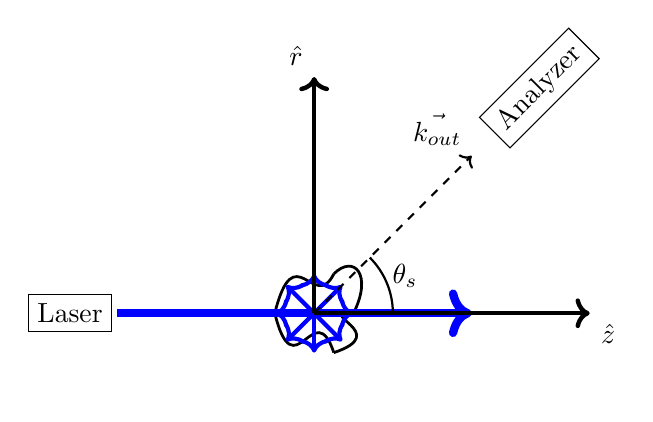
\begin{tikzpicture}
 
 		%Scattering Volume
 		\draw[line width=1pt] (0,0) .. controls (.25,1) and (.5,0) .. (.75,.5);
 		\draw[line width=1pt] (.75,.5) .. controls (1,.75) and (1.25,.5) .. (1,0);
 		\draw[line width=1pt] (1,0) .. controls(.5,0) and (1.5,-.25) .. (.75,-.5);
 		\draw[line width=1pt] (.75,-.5) .. controls (.5,.25) and (.25,-1) .. (0,0);
 
 		%Incident and Scattered Field Vectors
		\draw [->,line width=3pt,blue] (-2,0) -- (2.5,0);
 		\draw [->,line width=1.5pt,blue] (.5,0) -- (.5,.5);
 		\draw [->,line width=1.5pt,blue] (.5,0) -- (.146447,.5*.707107);
 		\draw [->,line width=1.5pt,blue] (.5,0) -- (.853553,.5*.707107);
 		\draw [->,line width=1.5pt,blue] (.5,0) -- (1,0);
 		\draw [->,line width=1.5pt,blue] (.5,0) -- (0,0);
 		\draw [->,line width=1.5pt,blue] (.5,0) -- (.5,-.5);
 		\draw [->,line width=1.5pt,blue] (.5,0) -- (.146447,-.5*.707107);
 		\draw [->,line width=1.5pt,blue] (.5,0) -- (.853553,-.5*.707107);
 
 		%Z-Axis
 		\draw[ultra thick,->] (.5,0) -- (4,0) node[anchor=north west] {$\hat{z}$};
 		\draw[ultra thick,->] (.5,0) -- (.5,3) node[anchor=south east] {$\hat{r}$};
 
 		%dashed Scattering Vector
 		\draw[thick, dashed,->] (.5,0) -- (2.5,2) node[anchor=south east] {$\vec{k_{out}}$};
 
 		%arc for scatter vector
 		\draw[thick] (1.5,0) arc (0:45:1);
 		\node[] at (1.654849,.478354) {$\theta_{s}$};
 
 		\node[draw, rotate=45] at (3.360077,2.860077) {Analyzer};
 		\node[draw] at (-2.6,0) {Laser};
 
 	\end{tikzpicture}
 	\caption{Generalized light scattering geometry}
 	\label{figure:scatterSetup}
 \end{figure}
 
It is important to quantify the length scales relevant to the scattering volume in order to justify the continuum treatment used in the derivation of \eqn\nolinebreak \ref{eqn:waveequation}. For a typical focused laser beam used in light scattering experiments, the beam waist may be on the order of $w_0 \sim 50$--$100~\mu$m, while the effective scattering length defined by the collection optics is on the order of $L \sim 1$--$5~\text{mm}$. This corresponds to a scattering volume of approximately
\begin{equation}
	V \sim \pi w_0^2 L \approx 10\text{--}150~\text{nL}.
\end{equation}

\noindent For a typical molecular liquid with number density in the ballpark of $n \sim 10^{13}~\text{nL}^{-1}$, the scattering volume lies well within the continuum limit.

This should be contrasted with the characteristic intermolecular spacing, $a \sim 0.3$--$0.5~\text{nm}$, which is many orders of magnitude smaller than both the optical wavelength ($\lambda \sim 500~\text{nm}$) and the spatial extent of the scattering volume. As a result, the measured scattering signal arises from the collective response of an enormous number of molecules, and fluctuations in the dielectric susceptibility emerge from statistically averaged molecular motions that are effectively uncorrelated on optical length scales. Within any fluid above absolute zero there will be local regions where bulk thermodynamic properties such as entropy, temperature, or pressure will fluctuate about the average value.  It is these fluctuations, as alluded to previously, that give rise to the scattering field.  Thus, it is reasonable to invoke hydrodynamic and thermodynamic theory to arrive at a model for the spectrum of light scattered from a simple fluid.  Such a model was first derived by Komarov and Fisher in their 1962 publication\cite{Komarov}. In this work Komarov adapted neutron scattering models derived by Leon van Hove in 1954 to describe light scattering spectra\cite{Hove}. It should be noted that this derivation is also provided in excellent detail by Berne and Pecora \nolinebreak \cite{Berne}.  The resulting spectrum of this scattered light was shown by Komarov to be proportional to the spatial and temporal Fourier transform of the generalized pair correlation function. While \sect \ref{sec:sctructualdesc} introduced the static radial distribution function describing equilibrium structure, it is necessary here to consider its dynamical extension. 

Following the work of van Hove, the static pair correlation function is generalized to the time-dependent van Hove correlation function $G(\vec{r},t)$, which describes the probability of finding a particle at position $\vec{r}$ at time $t$ given that a particle was located at the origin at time $t=0$. The dynamic structure factor $S(\vec{q},\omega)$ is then obtained as the spatial and temporal Fourier transform of $G(\vec{r},t)$. The scattered intensity may therefore be written as
\begin{equation}
	I^\prime\left(\vec{r},\omega\right)
	=
	I_0 N \omega^4 \sin^2{\gamma}\,
	S\left(\vec{q},\omega\right),
\end{equation}
\noindent where $I_0$ is the incident intensity, $N$ is the number of scatterers within the scattering volume, $\omega$ is the angular frequency of the incident field, and $\gamma$ is the angle between the induced dipole moment and the observation direction, giving rise to the characteristic dipole radiation pattern. Here $\vec{q} = \vec{k}_s - \vec{k}_i$ is the scattering wavevector.

This result is closely related to that for Rayleigh scattering from a diffuse gas, with the addition of the structure factor, $S\left(\vec{q},\omega \right)$, which contains information about the molecular dynamics of the system. Mountain later extended the results of Komarov and Fisher and through application of the linearized hydrodynamic equations, which include the continuity equation, Navier--Stokes, and energy-transport equations, derived a model for the frequency-dependent structure factor of a classical fluid comprised of spherically symmetric molecules as follows:
\begin{equation}
\centering
S\left(q,\omega \right )=\frac{c_p-c_v}{c_p}\frac{2\lambda q^2/\rho_0c_p}{\left(\lambda q^2/\rho_0c_p \right )^2+\omega^2}+\frac{c_v}{c_p}\left [ \frac{\Gamma q^2}{\left(\Gamma q^2 \right )^2+\left(\omega+C_0 q \right )^2}+ \frac{\Gamma q^2}{\left(\Gamma q^2 \right )^2+\left(\omega-C_0 q \right )^2}\right ].\label{eqn:simpleFluid}
\end{equation}
Here $\rho_0$, $c_p$, $c_v$, $C_0$, and $\lambda$ are the equilibrium density, specific heat at constant pressure, specific heat at constant volume, low frequency limit of the sound velocity, and the thermal conductivity respectively.\cite{Mountain2}  The first, left-most term of \eqn\nolinebreak \ref{eqn:simpleFluid} represents the broadened central peak of light scattering from entropy fluctuations which occur at constant pressure.  In a simple fluid, as there are no internal degrees of freedom, this takes the form of diffusion or breaking of nearest neighbor cages\textemdash \ie, structural relaxation.  The right-most term of \eqn\nolinebreak \ref{eqn:simpleFluid} represents light scattered by propagating acoustic waves.  As this is an adiabatic process, this occurs at constant entropy.  This term forms two peaks symmetrically located around the central peak with frequency shifts from $E_i$ proportionally to the speed of sound.  These are often referred to as the longitudinal acoustic modes.  This model is sufficient to describe the dynamics of a simple fluid in the sense described by Mountain: a single-component, monatomic system in which internal degrees of freedom may be neglected and the dynamics are governed entirely by density fluctuations. However, typical glass-forming systems possess additional internal and configurational degrees of freedom, giving rise to additional modes of structural relaxation beyond those captured by this description.

Many glass-forming systems are significantly more complex, exhibiting internal degrees of freedom, intermolecular hydrogen bonding, and other additional considerations.  Polymer systems can fold and flex.  Even simple molecular systems limited to van der Waals interactions, such as cumene, have rotational degrees of freedom that give rise to additional relaxation modes.  Such considerations will add to the complexity of this structure factor.  Mountain followed this previous work with a derivation of a structure factor accounting for internal degrees of freedom weakly coupled to the originally considered translational degrees of freedom via a single representative orientational relaxation time, $\tau$ as follows \cite{Mountain}: 

\begin{align}
\begin{split}
S\left(q,\omega \right )={}& \frac{c_p-c_v}{c_p}\frac{2\lambda q^2/\rho_0c_p}{\left(\lambda q^2/\rho_0c_p \right )^2+\omega^2}+\\
& \left[\frac{\left(c^2_\infty-c^2_0\right )k^2-\left(v^2/c^2_0-1 \right )\left(c^4_0/v^4\tau^2+c^2_0q^2\left(\frac{c_p-c_v}{c_p} \right ) \right )}{c^4_0/v^4\tau^2+v^2q^2}\right]\left[\frac{\frac{2c^2_0}{v^2\tau}}{\frac{c^4_0}{v^4\tau^2}+\omega^2} \right ] +\\
& \qquad \qquad \qquad \qquad \left[\frac{\left[1-\frac{c^2_0}{v^2}\left(\frac{c_p-c_v}{c_p} \right ) \right ]\left[v^2q^2+\frac{c^2_0}{v^2\tau^2} \right ]-\left(c^2_\infty-c^2_0 \right )q^2}{\frac{c^4_0}{v^4\tau^2}+\frac{v^2}{q^2}}
\right ]\times \\
& \qquad \qquad \qquad \qquad
\left[\frac{\Gamma_B}{\Gamma^2_B+\left(\omega-vq \right )^2}+\frac{\Gamma_B}{\Gamma^2_B+\left(\omega+vq \right )^2} \right ].
\end{split}\label{eqn:intdegfluid}
\end{align}
Here the longitudinal acoustic modes represented by the third term are structurally indistinguishable from the second term of \eqn\nolinebreak \ref{eqn:simpleFluid} though now the coefficient is $\tau$ dependent.  Likewise the first term, associated with translational diffusion, remains unchanged from before.  However, most notably, there now emerges a secondary central feature symmetric about the incident frequency, associated with this internal relaxation mode. Thus the orientational dynamics directly affect the structure of this central feature.  There is a vast amount of insight provided by this model.  However the primary consideration relevant to this work lies in this additional central term of \eqn\nolinebreak \ref{eqn:intdegfluid} above.  Consider the following simplified expression of this structure.
\begin{equation}
f\left(\omega \right )=\left(\frac{2\Gamma}{\Gamma^2+\omega^2} \right )\label{eqn:simplecentral}
\end{equation}
This function, as aforementioned, will be symmetric about the axis $\omega=0$ and will have a characteristic half width half maximum value of $\Gamma$ as shown in \fig \nolinebreak \ref{figure:centralstructure}.
\begin{figure}[!htbp]
	\centering
	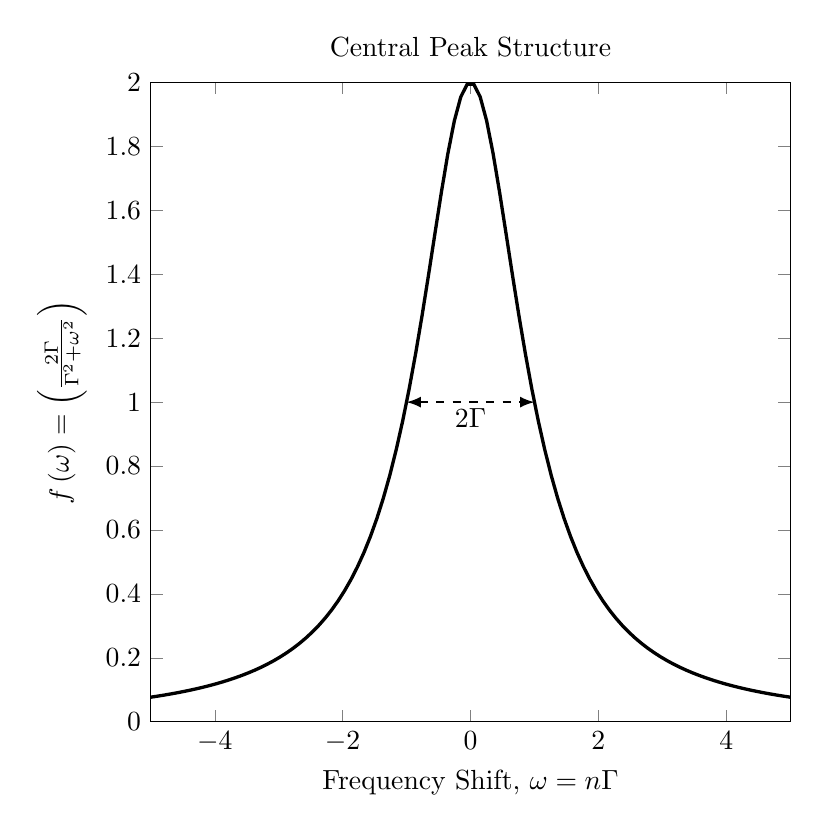
\begin{tikzpicture}[>=latex]
	
	\begin{axis}[
	samples=100,
	title={Central Peak Structure},
	width=.8\textwidth,
	height=.8\textwidth,
	xmin=-5,xmax=5,
	ymin=0,ymax=2,
	ylabel={$f\left(\omega \right )=\left(\frac{2\Gamma}{\Gamma^2+\omega^2} \right )$},
	xlabel={Frequency Shift, $\omega=n\Gamma$},
	]
	
	\addplot expression[black, very thick, solid,mark=none]{
		2/(1+x^2)}; 
	
	\draw[thick, dashed,<->] (-1,1) -- (1,1);
	\node[] at (0,.95) {$2\Gamma$};
		
	\end{axis}

	\end{tikzpicture}
	\caption{Here we have the generalized structure of the central features from \eqn\nolinebreak \ref{eqn:simpleFluid} and \nolinebreak \eqn\ref{eqn:intdegfluid}.  The x-axis here is in terms of multiples of the generalized parameter $\Gamma$ from \eqn\nolinebreak \ref{eqn:simplecentral} which also defines the half width-half maximum value for this feature.}
	\label{figure:centralstructure}
\end{figure}
Placing aside the specific values of any particular bulk thermodynamic property, both the first and second term of \eqn\nolinebreak \ref{eqn:intdegfluid} have the same basic structure in this model.  Generally speaking, the structural relaxation associated with translational and orientational diffusion can occur on vastly different timescales however both will contribute to the width of this central feature.  It bears mention that, for a simple monatomic fluid, only the translational diffusion term contributes to this central feature and $\Gamma=\frac{\lambda}{\rho_0c_p}q^2=D_Tq^2$ where $D_T$ is the thermal diffusivity and there exists a dependency on the scattering vector.  However, if the orientational diffusion contribution dominates the width of the central feature then $\Gamma=\frac{{c_0}^2}{v^2\tau}=\frac{D_\tau}{\tau}$ and there is no dependence on the scattering vector.

The work of Demoulin, Montrose, and Ostrowsky provides valuable insights and foundational support for understanding the scattering phenomena described in this chapter. Specifically, Demoulin \etal employed digital-correlation spectroscopy, analogous to photon correlation spectroscopy (PCS) utilized in this dissertation, to investigate structural relaxation in viscous liquids over time scales from $\SI{1}{\micro\second}$ to $\SI{1}{\second}$. Their work explicitly analyzed the Rayleigh scattering of light from undercooled glycerol, relating the measured correlation function to the isothermal structural relaxation dynamics of the liquid\cite{Demoulin}.

Demoulin \etal characterized three distinct regimes governing the Rayleigh line shape arising from density fluctuations: thermal diffusion dominance, structural relaxation dominance, and an intermediate regime involving contributions from both processes. Of particular interest here is what Demoulin \etal described as the "Mountain component," which appears prominently under conditions where the structural relaxation timescale is significantly slower than the phonon modes but faster than thermal diffusion processes.

This Mountain component corresponds directly to the central feature described earlier in the structural factor from \eqn\nolinebreak \ref{eqn:intdegfluid}, particularly when orientational diffusion significantly influences its width. Demoulin \etal modeled the relaxation function using a Cole-Davidson distribution—precisely the approach taken in this dissertation—to quantify the relaxation dynamics, further validating the methodology adopted here. Their analysis determined that the Cole-Davidson distribution, characterized by a width parameter, provided a robust fit for their data.

Thus, the work presented in this dissertation parallels Demoulin \etal’s in both the choice of methodology (PCS) and the theoretical framework (Cole-Davidson distribution), thereby establishing continuity and credibility in the application of these techniques to characterize structural relaxation in glass-forming liquids. Furthermore, Demoulin \etal's findings underscore the importance and practicality of employing digital autocorrelation techniques to probe relaxation phenomena, reinforcing the methodologies implemented throughout this dissertation.

\section{Mathematical Models}
\label{sec:models}

In analyzing experimental data from dynamic light scattering experiments, it becomes necessary to implement mathematical models to characterize structural relaxation processes accurately. Four commonly used models—Debye relaxation, Cole-Cole, Cole-Davidson, and Williams-Watts—will be introduced, described, and compared in this section, with emphasis on their typical usage in either the time or frequency domain, and the interrelation between domains provided by Lindsey and Patterson.

\subsection{Debye Relaxation}

The Debye relaxation model represents the simplest case, assuming a single exponential decay characterizes the relaxation process. In the time domain, this corresponds to:

\begin{equation}
	\phi(t) = e^{-t/\tau_0}.
\end{equation}

\noindent where $\tau_0$ is a single characteristic relaxation time. In the frequency domain, Debye relaxation is described by:

\begin{equation}
	\phi(\omega) = \frac{1}{1 + i\omega\tau_0}.
\end{equation}

\noindent This model assumes a uniform relaxation process without distribution of relaxation times. Although appealing for simplicity, the Debye model fails to describe the complex relaxation behaviors observed in most glass-forming liquids.

\subsection{Cole--Cole Relaxation}

Recognizing deviations from ideal Debye behavior, the Cole--Cole model introduces a phenomenological broadening of the relaxation time spectrum, characterized by an additional parameter $\alpha$:

\begin{equation}
	\phi(\omega) = \frac{1}{1+(i\omega\tau_{cc})^{1-\alpha}}, \quad 0 \le \alpha < 1.
\end{equation}

\noindent where $\tau_{cc}$ is a characteristic relaxation time and $\alpha$ describes the deviation from single-exponential (Debye) relaxation. The limiting cases are instructive. For $\alpha = 0$, the expression reduces to the Debye model, corresponding to a single relaxation time and yielding a perfect semicircle when the imaginary component of the susceptibility is plotted against the real component. In contrast, as $\alpha \rightarrow 1$, the frequency dependence is suppressed and $\phi(\omega)$ approaches a constant, reflecting the absence of a well-defined relaxation process.

For intermediate values of $\alpha$, the response cannot be described by a single relaxation time. Instead, the Cole--Cole form corresponds to a distribution of relaxation times centered around $\tau_{cc}$. This behavior is most clearly visualized in a Cole--Cole plot, where increasing $\alpha$ leads to a symmetric depression of the semicircular response, as shown in \fig\nolinebreak\ref{fig:DebyeColeCole}.

\begin{figure}[!htbp]
	\centering
	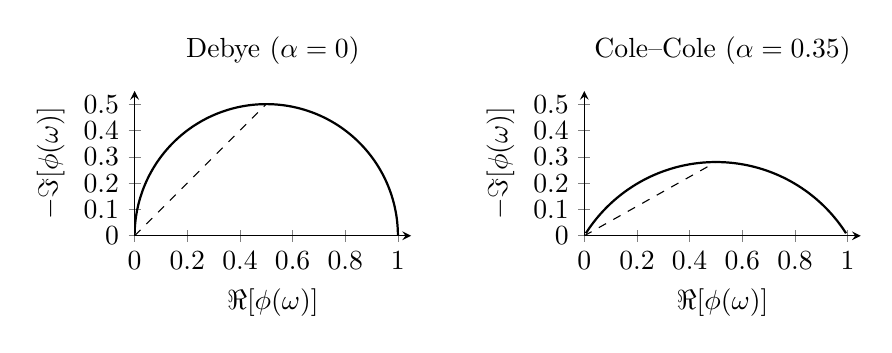
\begin{tikzpicture}
		
		\begin{groupplot}[
			group style={
				group size=2 by 1,
				horizontal sep=2.2cm
			},
			width=0.42\textwidth,
			height=0.32\textwidth,
			xmin=0, xmax=1.05,
			ymin=0, ymax=0.55,
			axis lines=left,
			axis equal image,
			xlabel={$\Re[\phi(\omega)]$},
			ylabel={$-\Im[\phi(\omega)]$},
			xtick={0,0.2,0.4,0.6,0.8,1.0},
			ytick={0,0.1,0.2,0.3,0.4,0.5},
			every axis plot/.append style={thick, black},
			domain=-3:3,
			samples=300,
			unbounded coords=jump
			]
			
			% ---------------- Debye ----------------
			\nextgroupplot[
			title={Debye ($\alpha=0$)}
			]
			
			\addplot[smooth]
			(
			{1/(1 + (10^x)^2)},
			{(10^x)/(1 + (10^x)^2)}
			);
			
			\addplot[dashed, thin] coordinates {(0,0) (0.5,0.5)};
			
			% ---------------- Cole-Cole ----------------
			\nextgroupplot[
			title={Cole--Cole ($\alpha=0.35$)}
			]
			
			\addplot[smooth]
			(
			{ (1 + (10^x)^0.65*cos(deg(0.65*pi/2))) /
				((1 + (10^x)^0.65*cos(deg(0.65*pi/2)))^2 + ((10^x)^0.65*sin(deg(0.65*pi/2)))^2) },
			{ ((10^x)^0.65*sin(deg(0.65*pi/2))) /
				((1 + (10^x)^0.65*cos(deg(0.65*pi/2)))^2 + ((10^x)^0.65*sin(deg(0.65*pi/2)))^2) }
			);
			
			\addplot[dashed, thin] coordinates {(0,0) (0.50,0.28)};
			
		\end{groupplot}
		
	\end{tikzpicture}
	\caption{Generalized representations of relaxation in a Cole--Cole plot. The case $\alpha = 0$ recovers simple Debye behavior, yielding a perfect semicircle. For $\alpha = 0.35$, the response exhibits a depressed semicircle, reflecting symmetric broadening of the distribution of relaxation times. Dashed lines are drawn from the origin to the peak of each arc, which occurs at $\omega\tau = 1$ in both cases, and emphasize the reduction in slope associated with increasing $\alpha$.}
	\label{fig:DebyeColeCole}
\end{figure}

\noindent This symmetric broadening reflects the presence of multiple relaxation pathways with comparable weights, rather than a single dominant timescale. While the Cole--Cole model captures symmetric deviations from Debye behavior, many glass-forming liquids exhibit asymmetric broadening of the relaxation spectrum. This behavior is more accurately described by the Cole--Davidson model, which will be discussed subsequently.

\subsection{Cole--Davidson Relaxation}

The Cole--Davidson model extends Debye relaxation by introducing an asymmetric broadening of the relaxation time distribution, characterized by the parameter $\beta$:

\begin{equation}
	\phi(\omega) = \frac{1}{(1 + i\omega\tau_{cd})^{\beta}}, \quad 0 < \beta \le 1.
	\label{eqn:ColeDavidson}
\end{equation}

\noindent where $\tau_{cd}$ is a characteristic relaxation time and $\beta$ describes the deviation from single-exponential (Debye) relaxation.

The limiting cases are again instructive. For $\beta = 1$, the expression reduces to the Debye model, corresponding to a single relaxation time and yielding a perfect semicircle, as in the case $\alpha = 0$ for the Cole--Cole model discussed above. As $\beta$ decreases below unity, the relaxation spectrum becomes increasingly asymmetric. In the limit $\beta \rightarrow 0$, the frequency dependence is suppressed and the response approaches a constant, analogous to the $\alpha \rightarrow 1$ limit of the Cole--Cole model.

For intermediate values of $\beta$, the response cannot be described by a single relaxation time. Instead, the Cole--Davidson form corresponds to a distribution of relaxation times with a pronounced tail toward longer relaxation times. This behavior is most clearly visualized in a Cole--Davidson plot, where decreasing $\beta$ leads to an asymmetric distortion of the semicircular response, as shown in \fig\nolinebreak\ref{fig:DebyeColeDavidson}.

\begin{figure}[!htbp]
	\centering
	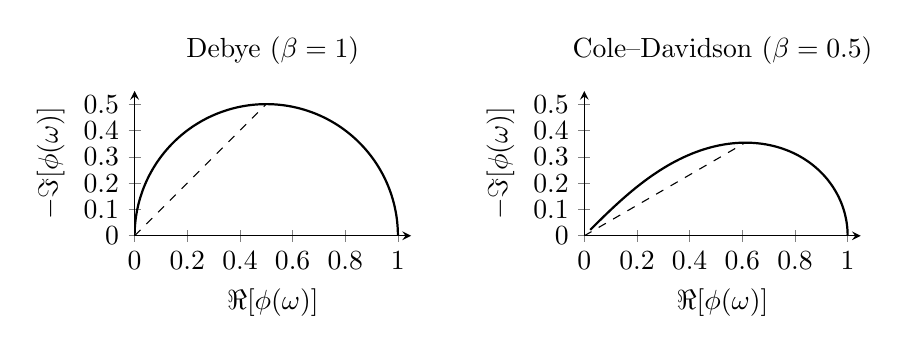
\begin{tikzpicture}
		
		\begin{groupplot}[
			group style={
				group size=2 by 1,
				horizontal sep=2.2cm
			},
			width=0.42\textwidth,
			height=0.32\textwidth,
			xmin=0, xmax=1.05,
			ymin=0, ymax=0.55,
			axis lines=left,
			axis equal image,
			xlabel={$\Re[\phi(\omega)]$},
			ylabel={$-\Im[\phi(\omega)]$},
			xtick={0,0.2,0.4,0.6,0.8,1.0},
			ytick={0,0.1,0.2,0.3,0.4,0.5},
			every axis plot/.append style={thick, black},
			domain=-3:3,
			samples=300,
			unbounded coords=jump
			]
			
			% ---------------- Debye ----------------
			\nextgroupplot[
			title={Debye ($\beta=1$)}
			]
			
			\addplot[smooth]
			(
			{1/(1 + (10^x)^2)},
			{(10^x)/(1 + (10^x)^2)}
			);
			
			\addplot[dashed, thin] coordinates {(0,0) (0.5,0.5)};
			
			% ---------------- Cole-Davidson ----------------
			\nextgroupplot[
			title={Cole--Davidson ($\beta=0.5$)}
			]
			
			\addplot[smooth]
			(
			{(1 + (10^x)^2)^(-0.25) * cos(0.5*atan(10^x))},
			{(1 + (10^x)^2)^(-0.25) * sin(0.5*atan(10^x))}
			);
			
			\addplot[dashed, thin] coordinates {(0,0) (0.612,0.354)};
			
		\end{groupplot}
		
	\end{tikzpicture}
	\caption{Generalized representations of relaxation in a Cole--Davidson plot. The case $\beta = 1$ recovers simple Debye behavior, yielding a perfect semicircle. For $\beta = 0.5$, the response exhibits an asymmetric distortion of this semicircle, reflecting a broadened distribution of relaxation times with a pronounced tail toward longer relaxation times. Dashed lines are drawn from the origin to the peak of each arc and emphasize the increasing asymmetry with decreasing $\beta$.}
	\label{fig:DebyeColeDavidson}
\end{figure}

\noindent This asymmetric broadening reflects the presence of relaxation pathways that extend to longer timescales, rather than a symmetric distribution about a central value. While the Cole--Cole model captures symmetric deviations from Debye behavior, the Cole--Davidson form is often more appropriate for glass-forming liquids, where such asymmetric relaxation spectra are commonly observed. Demoulin \etal successfully employed this model to describe structural relaxation in viscous liquids such as glycerol using digital-correlation spectroscopy in the time domain. We will later do likewise.

\subsection{Kohlrausch--Williams--Watts (KWW) Relaxation}

The Kohlrausch--Williams--Watts (KWW) model of \eqn \ref{eqn:KWW}, commonly referred to as the stretched exponential, is widely used to describe relaxation processes in the time domain. This form was first introduced by Kohlrausch in 1854 in the context of charge relaxation in capacitive systems \cite{Kohlrausch1854}, but was largely overlooked until its reintroduction by Williams and Watts in 1970 in the study of dielectric relaxation \cite{Williams}. The terminology ``stretched exponential'' was later popularized by Chamberlin \cite{Chamberlin1984}.

\begin{equation}
	\phi(t) = e^{-(t/\tau_{ww})^{\beta_{ww}}}, \quad 0 < \beta_{ww} \le 1
	\label{eqn:KWW}
\end{equation}

\noindent In \eqn \ref{eqn:KWW}, $\tau_{ww}$ is a characteristic relaxation time and $\beta_{ww}$ quantifies the degree of stretching relative to a simple exponential decay.

The limiting case $\beta_{ww} = 1$ recovers Debye relaxation, corresponding to a single relaxation time. For $\beta_{ww} < 1$, the decay becomes increasingly stretched, reflecting a broad distribution of relaxation times associated with cooperative and heterogeneous dynamics. Such non-exponential relaxation behavior is a hallmark of glass-forming systems and has been extensively discussed in the context of dynamic heterogeneity \cite{Bohmer1993,Ediger2000}.

Unlike the Cole--Cole and Cole--Davidson models, which are defined in the frequency domain, the KWW form is naturally expressed in the time domain. Its corresponding frequency-domain response does not, in general, admit a simple closed-form expression and is therefore most conveniently obtained numerically. The resulting spectrum is asymmetric and often resembles a Cole--Davidson-like response, as shown in \fig \ref{fig:KWWTransform}. This apparent similarity reflects the fact that both forms capture a distribution of relaxation times skewed toward longer times, although they arise from fundamentally different functional representations.

\begin{figure}[!htbp]
	\centering
	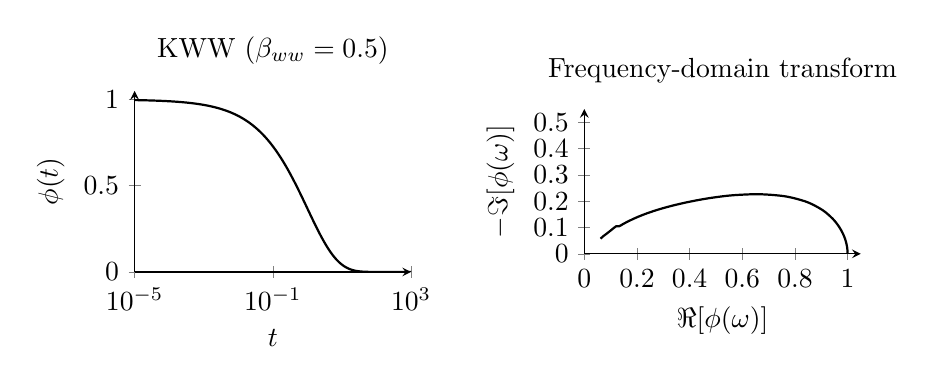
\begin{tikzpicture}
		
		\begin{groupplot}[
			group style={
				group size=2 by 1,
				horizontal sep=2.2cm
			},
			width=0.42\textwidth,
			height=0.32\textwidth,
			every axis plot/.append style={thick, black},
			]
			
			% ---------------- KWW time domain ----------------
			\nextgroupplot[
			title={KWW ($\beta_{ww}=0.5$)},
			xmode=log,
			xmin=1e-5, xmax=1e3,
			ymin=0, ymax=1.05,
			axis lines=left,
			xlabel={$t$},
			ylabel={$\phi(t)$},
			domain=-5:3,
			samples=300
			]
			
			\addplot[smooth]
			(
			{10^x},
			{exp(-sqrt(10^x))}
			);
			
			% ---------------- Frequency-domain transform ----------------
			\nextgroupplot[
			title={Frequency-domain transform},
			xmin=0, xmax=1.05,
			ymin=0, ymax=0.55,
			axis lines=left,
			axis equal image,
			xlabel={$\Re[\phi(\omega)]$},
			ylabel={$-\Im[\phi(\omega)]$},
			xtick={0,0.2,0.4,0.6,0.8,1.0},
			ytick={0,0.1,0.2,0.3,0.4,0.5},
			]
			
			\addplot[smooth] coordinates {
				(0.999988,0.002000)
				(0.999976,0.002806)
				(0.999954,0.003936)
				(0.999909,0.005521)
				(0.999820,0.007742)
				(0.999647,0.010853)
				(0.999308,0.015201)
				(0.998647,0.021258)
				(0.997374,0.029641)
				(0.994962,0.041108)
				(0.990478,0.056510)
				(0.982358,0.076687)
				(0.968061,0.102274)
				(0.943841,0.132931)
				(0.904773,0.166306)
				(0.845648,0.196948)
				(0.763693,0.218396)
				(0.663280,0.226468)
				(0.559895,0.222229)
				(0.472140,0.211213)
				(0.401810,0.198427)
				(0.345814,0.185875)
				(0.300736,0.174013)
				(0.263766,0.162799)
				(0.232945,0.152103)
				(0.206852,0.141843)
				(0.184428,0.131986)
				(0.164870,0.122524)
				(0.147549,0.113457)
				(0.132000,0.104786)
				(0.121554,0.105170)
				(0.103111,0.091049)
				(0.087225,0.078493)
				(0.072632,0.067513)
				(0.061778,0.057805)
			};
			
		\end{groupplot}
		
	\end{tikzpicture}
	\caption{Generalized representations of KWW relaxation. Left: the stretched exponential form in the time domain for $\beta_{ww}=0.5$. Right: the corresponding frequency-domain response obtained by numerical transformation of the KWW function, shown in a Cole--Cole-style representation. The resulting spectrum is asymmetric and resembles a Cole--Davidson-like arc, but does not arise from the Cole--Davidson functional form itself.}
	\label{fig:KWWTransform}
\end{figure}

Although the Cole--Davidson and KWW models are typically employed in the frequency and time domains, respectively, Lindsey and Patterson established a detailed relationship between these two forms \cite{Lindsey}. Their work provides empirical relations allowing parameters extracted in one domain to be related to those in the other, facilitating consistent comparison and interpretation across different experimental techniques.

\subsection{Comparison, Contrast, and Justification}

The Debye model, while simple, rarely suffices for complex fluid relaxations. The Cole--Cole model introduces symmetric broadening suitable for moderately complex systems, while the Cole--Davidson form captures pronounced asymmetry in the relaxation spectrum. The Williams--Watts model, though defined in the time domain, produces a similarly asymmetric response.

Importantly, the Cole--Davidson and Williams--Watts models arise from fundamentally different underlying distributions of single relaxation times. Despite this, both have been shown to provide excellent fits to $\alpha$-relaxation data in glass-forming liquids. This suggests a relative insensitivity of experimental observables to the precise form of the underlying distribution, provided that the essential features of broadening and asymmetry are captured.

As discussed in \sect\nolinebreak\ref{sec:probes} and illustrated in \fig\nolinebreak\ref{figure:Probes}, no single experimental technique spans the full dynamic range over which structural relaxation occurs. Instead, multiple probes are required, yielding data in both the frequency domain (\eg, dielectric and Brillouin spectroscopy) and the time domain (\eg, photon correlation spectroscopy). As a result, consistent interpretation of relaxation dynamics requires that parameters extracted from one representation be meaningfully related to those obtained in another. Lindsey and Patterson established empirical relationships between time- and frequency-domain descriptions, providing a framework for such comparisons \cite{Lindsey}. However, Demoulin instead chose to directly fit time-domain autocorrelation data using a transformed Cole--Davidson form \cite{Demoulin}. We will adopt Demoulin's approach in analyzing our own time-domain data in the chapters that follow.

\section{Free-Volume Theory}\label{sec:freeVolume}

The concept of free-volume as a mechanism to explain viscosity was first postulated as far back as 1913 when Batschinski proposed a linear relationship between thermal expansion and viscosity \nolinebreak\cite{Batschinski}. Though this linear model will obviously suffice over any sufficiently small thermodynamic range, it fails to adequately describe data from high temperatures down through a glass transition.  However the general idea of describing viscosity in terms of solid molecular units passing through regions of free-volume is certainly conceptually appealing and was gaining more traction in the literature in the early fifties.  Though Batschinski's model was known by this time to be insufficient to describe viscosity behavior beyond a first approximation, and certainly would only be applicable far from any glass transition where viscosity is rapidly diverging, there was no reason to believe the concept of free-volume was invalid.  The main competing theory of viscosity at the time was the rate theory proposed by Henry Eyring, which one may assert is physically equivalent to free-volume theory though couched in terms of the energy fluctuations associated with creating that free-volume\textemdash in the simplest terms, pushing nearest neighbors out of the way \nolinebreak\cite{Eyring}.  Eyring proposed that viscosity of any non-associated liquid, to the extent that structural relaxation is assumed to be an energetic process which involves breaking free of potential wells created by neighboring molecules, may be treated in much the same way as any chemical process activated by thermal energy fluctuations and should be well described by a Boltzman-like distribution involving a single activation energy, $E_0$, and of the following form:

\begin{equation}
	\eta=\frac{Nd}{V}\left(2\pi m k_B T\right)^{\frac{1}{2}}\exponential{\frac{E_0}{k_B T}}
	\label{eqn:Eyring}
\end{equation} 

It is not surprising that an associated liquid such as glycerol might fail to be well described by this Arrhenius model.  However even most non-associated fragile glass-forming systems also conform well to the phenomenological VTF equation.  Thus if one is to overcome the apparent discrepancy between Eyring's rate theory of \eqn\nolinebreak \ref{eqn:Eyring} above and the VTF equation, the functional dependence of the activation energy on temperature must be of the form $E\left(T\right)\propto \frac{T}{T-T_\infty}$, where $T_\infty$ is the zero mobility temperature at which viscosity becomes infinite. This requirement rather diminishes the physical grounding of the Eyring rate theory as it offers no explanation as to why the temperature dependence of activation energy should take this form.  Some have tried to link the temperature dependence of activation energy with local entropy fluctuations and met with some level of success \nolinebreak\cite{Frenkel}.  In fact such a rate theory is the foundation for the Adam-Gibbs equation which has been heavily implemented to describe enthalpy relaxation in many glass-forming systems \nolinebreak\cite{Adam,Hodge}. However the conceptual simplicity and elegance of a free-volume description may suggest that a non-linear free-volume equation, beyond that suggested by Batschinski, may be the most physically meaningful approach to describing viscosity of these non-Arrhenius systems.  It was during the same year of 1951 that Doolittle published his work describing viscosity of n-paraffin hydrocarbons \via an exponential free-volume model, similar in form to the Eyring rate theory, yet dependent upon the relative free-space, $\frac{v_f}{v_0}$ within a bulk liquid rather than an activation energy,

\begin{equation}
	\eta=A\exponential{B\left(\frac{v_f}{v_0}\right)},
	\label{eqn:Doolittle}
\end{equation} 

\noindent where $v_f$ is the volume of free-space per unit of liquid and $v_0$ is that free-volume density specifically evaluated at some reference temperature\textemdash often absolute zero \nolinebreak\cite{Doolittle}.  

This is useful as it circumvents the need to explain any functional dependence of a potentially complicated distribution of activation energies and attacks the problem from an arguably conceptually simpler standpoint of free-volume\textemdash is there sufficient free-volume, on average, for molecular mobility to progress at a given rate.  Only thermal expansion needs to be considered as all other parameters are temperature independent. The Doolittle expression for free-volume of \eqn\nolinebreak \ref{eqn:Doolittle} above also provided the groundwork for Williams, Landel, and Ferry to explain the temperature dependence of kinetic constants as a function  of temperature near the glass transition \nolinebreak\cite{Williams2}.  It was a major contribution that launched the free-volume model into common implementation.  However Eyring's rate theory explanation was certainly not supplanted by a free-volume approach.  Again, structural fluctuations that give rise to local free-volume, \ie, the opening of a path through which a caged molecule might diffuse, must be energetically accessible as must be the diffusion process itself.  It should be unsurprising that a model relying on a temperature independent single activation energy to describe what, even in simple liquids, amounts to several independent modes of relaxation all of which may have strong temperature dependence, especially as the glass transition is approached, would prove to be every bit as insufficient as Batschinski's linear free-volume model.  Eyring's model failed to sufficiently describe diffusion even in some simple crystalline systems \nolinebreak\cite{Zener}.  

Consider again the potential energy landscape of \fig \nolinebreak \ref{figure:landscape} way back in \chap\nolinebreak \ref{chap:Introduction}. Though, to some extent, structural relaxation may be entirely entropy driven as regions held at constant energy may still explore equipotential surfaces, moving from one local minimum within the energy landscape to another will be an energy activated process. Particularly as one approaches a state here described as an ideal glass, the activation energy associated with hopping between adjacent potential wells will be strongly temperature dependent and the complexity of the parameter space implies there will be a near uniform distribution of potential paths through the parameter space corresponding to physical modes of structural relaxation.  Thus Henry Eyring's description of viscosity as an energy activated process underlies the concept of free-volume.  Bueche makes note, in his contemporary work on the segmental mobility of polymers, that one is left free to conceptualize relaxation processes in terms of the activation energy, $\epsilon$, needed to break free of nearest neighbor cages or equivalently in terms of an activation volume, $\Delta V$, needed for a molecular unit, or sub-molecular in the case of polymer chains, to pass through \nolinebreak\cite{Bueche}.  Bueche also importantly notes that, as previously alluded to by Davidson and Cole regarding the failure of the Debye hydrodynamic model to sufficiently explain the relaxation processes of glycerol, an activation volume, $\Delta V$, need not be on the order of the molecular volume as relaxation modes may involve cooperative motions of sub-molecular units.  

Bueche's desire to connect free-volume theory, which since the contribution of Doolittle had been shown to aptly model viscous behavior of many liquids over a much larger range of temperatures than when first proposed as a linear model by Batschinski, with the Eyring rate theory is quite understandable.  Eyring's rate theory of viscosity, though experimentally found wanting, was strongly rooted in a first-principles derivation and shares an elegant symmetry with the well established thermodynamic theory of chemical reaction rates.  If viscosity is, in fact, an energy activated process it should be governed by similar expressions to those governing chemical reactions.  Though it may be convenient to model viscosity in terms of free-volume, Bueche argues that the creation of this free-volume comes at an energetic cost.  The free-volume model proposed by Doolittle, though experimentally successful, falls short of the Eyring rate theory in its lack of any theoretical explanation\textemdash the exponential form of \eqn\nolinebreak \ref{eqn:Doolittle} being entirely phenomenological.  

A first-principles theoretical derivation of Doolittle's free-volume model was finally provided in 1959 \via the work of Cohen and Turnbull \nolinebreak\cite{Cohen}. To accomplish this, Cohen and Turnbull envisioned an entropic rather than energetic activation behind structural relaxation. Consider again the parameter space idealized by \fig \nolinebreak \ref{figure:landscape} as the n-dimensional surface that would exist for any real liquid.  The energetic processes described by Bueche and Eyring may not be necessary to navigate a sufficiently complex parameter space.  Couched in terms of the energy landscape picture, Cohen and Turnbull might suggest that one consider that what perhaps appears to be an insurmountable energy barrier between two adjacent potential wells in \fig \nolinebreak \ref{figure:landscape} in the absence of some introduced activation energy, $\epsilon$, may in fact be accessible \via multiple paths along equipotential surfaces in higher dimensional parameter space.  Evolution along these equipotential surfaces correspond to pure entropy fluctuations at constant energy and can be physically interpreted as a rearrangement of existing free-volume within the bulk material.  

Cohen and Turnbull do well to point out that the diffusion constant for spherical particles dispersed in a viscous medium is inversely related to viscosity \via the Stokes-Einstein relation,
\begin{equation}
	D=\frac{k_B T}{3\pi a_0 \eta},
	\label{eqn:StokesEinstien}
\end{equation}

\noindent where $a_0$ is the hard sphere cross-section.  Though this is derived in the context of low number density macroscopic spherical particles suspended in a viscous fluid, rather than the self diffusion of a pure liquid, it is still contextually relevant to the latter.  In fact the use of nano-particles suspended in a liquid to serve as a probe of the molecular dynamics of the host liquid certainly appears in the literature and was considered as a possible method for extending photon correlation spectroscopy into the diamond anvil cell, the results of which are described in \chap\nolinebreak \ref{chap:PCS}.  Suffice it to say for now that there was concern regarding the light arising from density fluctuations  within a pure liquid from the very small volume of a diamond anvil cell being sufficient in intensity for photon correlation spectroscopy.  As such it was considered that sufficiently small probe particles, perhaps within an order of magnitude of the molecular size of the liquid under study, might provide a sufficient scattering intensity and their diffusion would approximate, or at least track with, that of the molecular self diffusion for the host liquid.  

This idea was in part inspired by the work of Caronna \etal who implemented x-ray scattering from suspended nano-particles to probe the dynamics of a glass-forming liquid \nolinebreak\cite{Caronna}.  They found that at higher temperatures the particles undergo Brownian motion as predicated by \eqn\nolinebreak \ref{eqn:StokesEinstien} above however, as the glass transition is approached, the probe particles exhibit what the authors referred to as "hyperdiffusive behavior" which they suggest is due to the emergence of cooperative motions of the host liquid.  It may be further suggested that, while approaching the glass transition, the effective size of the molecular units involved in structural relaxation increase accordingly as cooperative domains of the host liquid increase in size.  This hyperdiffusive behavior will emerge as the size of these cooperative domains approach that of the probe particles.

The point to be had here is that, to the extent that a pure liquid can be modeled as consisting of hard spheres of radius $a_0$, self diffusion within a pure liquid should be well modeled by the Stokes-Eienstein relationship.  Cohen and Turnbull assumed that this description would remain valid through the glass transition. However, later work, including that of Caronna \etal, suggests that this assumption may break down due to the emergence of cooperative dynamics. As the glass transition is approached, the effective size of the relaxing regions becomes temperature dependent and increases, reflecting the growing influence of collective molecular rearrangements. The emergence of cooperative domains and their role regarding structural relaxation within glass-forming systems was not so well understood at this time.  None the less, in the case of self diffusion from the perspective of free-volume, the effective size of the relaxing units, whether they be sub-molecular or large cooperative domains, will be intrinsically associated with the viscosity $\eta$. It is reasonable to assert that, no matter the functional form, to first approximation self diffusion within a pure liquid should be inversely proportional to the viscosity of the liquid.  

The question that remains is whether this viscosity and diffusion result from energy activated processes or pure entropy fluctuations involving a rearrangement of free-volume within the bulk material.  Cohen and Turnbull assumes the latter.  What will follow here is Cohen and Turnbull's derivation of Doolittle's free-volume formula from first principles that exactly correlates with that of the energy activated rate theory of Eyring\textemdash the only difference being that energy constraints and statistical distributions are replaced with equivalent free-volume constraints and distributions.  However it should perhaps be pointed out that, though Cohen and Turnbull here describe the process of diffusion, or equivalently viscosity, as arising from pure entropy fluctuations, the derivation that follows does not preclude free-volume being created or destroyed as the result of energetic processes.  Generally speaking, a substance whose constituent molecules have sufficient average energy, $k_B T$, to exist in a liquid state will manifest local thermal fluctuations on the order of the heat of fusion giving rise to the creation of vacancies within the liquid\textemdash \ie, free-volume.  Thus, arguably, one should not view free-volume theory as an alternative to an energy activated rate theory, but rather simply a more natural means of expressing such a theory \via circumventing the need to parameterize the complicated distribution of temperature dependent activated processes that may give rise to the creation of free-volume.

The total free-volume of a bulk liquid, having average thermal energy $k_B T$, will undoubtedly fluctuate, however the expectation value of that total free-volume will be as solidly defined as any thermodynamic parameter.  Cohen and Turnbull define the average free-volume per molecule, analogous to the average thermal energy per molecule defined by Eyring, as $\nu_f=V_f/N$, where $V_f$ is the total free-volume and $N$ is the total number of particles in the bulk.  Though it was reasonable for Eyring to assume the total energy of an isolated system is constant, there certainly will be fluctuations in the total free-volume, $V_f$, even in an isolated system, however such fluctuations will be of negligible magnitude and thus would likely prove inconsequential to any derivation.  In any case such fluctuations remain irrelevant as $V_f$ is either assumed to be the time-average value of the total free-volume or, assuming ergodicity, $\nu_f$ is simply defined as the ensemble average of local free-volume over the entirety of the bulk at any given instant.  All of that being sufficiently addressed, we can move on to the derivation of Doolittle's free-volume model derived in a similar fashion as by Cohen and Turnbull. 

\subsection{Derivation of a Free Volume model}\label{sec:freeVolumederive}

Let us consider a bulk fluid of finite volume.  In general, there may be an infinite number of ways in which nearest neighbors to any particular molecule may be arranged within the fluid.  However there is going to be a net free-volume, $V_f$, within the bulk at any given time which can be thought to be divided among $N$ constituent molecular (or sub-molecular) units.  Consider a set of small yet discrete increments of free-volume, $\Delta\nu$, that may be attributed to the $i^{th}$ molecule within the bulk as illustrated in \fig \nolinebreak \ref{figure:freeVolume}.  

%Data Array for Free-Volume figure
\def\data{% the data
	1 0
	2 0
	4 0
	5 0
	6 0
	9 0
	0 1
	0 3
	0 7
	9 3
	9 4
	9 5
	1 9
	2 9
	3 9
	4 9
	7 9
}
\readarray\data\dataFVgrey[4,2] %read the data to for grey balls at border
\def\data{% the data
	2 5
}
\readarray\data\dataFVorange[4,2] %read the data to for orange balls 2deltav
\def\data{% the data
	1 4
	3 5
	3 4
	4 8
	4 5
	5 1
}
\readarray\data\dataFVred[4,2] %read the data to for red balls 3deltav
\def\data{% the data
	1 6
	1 3
	2 8
	2 3
	3 6
	4 7
	4 4
	5 8
	7 2
	8 3
}
\readarray\data\dataFVblue[4,2] %read the data to for blue balls 4deltav
\def\data{% the data
	1 7
	1 5
	5 2
	5 5
	5 7
	7 1
	8 1
}
\readarray\data\dataFVgreen[4,2] %read the data to for green balls 5deltav
\def\data{% the data
	2 2
	4 2
	6 5
	7 3
	7 6
	7 7
	8 8
}
\readarray\data\dataFVviolet[4,2] %read the data to for blue balls 6violet

\begin{figure}[!htbp]
	\centering
	\begin{tikzpicture}
		
		\foreach \y in {0,...,10}
		{\draw[] (0,\y)--(10,\y);
		}
		\foreach \x in {0,...,10}
		{\draw[] (\x,0)--(\x,10);
		}
		\foreach \j in {1,...,17}
		{\shade[ball color = gray!40, opacity = 0.4] (\dataFVgrey[\j,1]+.5,\dataFVgrey[\j,2]+.5) circle (.5cm);	
		}
		
		\foreach \j in {1,...,1}
		{\shade[ball color = orange, opacity = 0.4] (\dataFVorange[\j,1]+.5,\dataFVorange[\j,2]+.5) circle (.5cm) node[anchor=center]{$2$};	
		}
		
		\foreach \j in {1,...,6}
		{\shade[ball color = red, opacity = 0.4] (\dataFVred[\j,1]+.5,\dataFVred[\j,2]+.5) circle (.5cm) node[anchor=center]{$3$};	
		}
		
		\foreach \j in {1,...,10}
		{\shade[ball color = blue, opacity = 0.4] (\dataFVblue[\j,1]+.5,\dataFVblue[\j,2]+.5) circle (.5cm) node[anchor=center]{$4$};	
		}
		
		\foreach \j in {1,...,7}
		{\shade[ball color = green, opacity = 0.4] (\dataFVgreen[\j,1]+.5,\dataFVgreen[\j,2]+.5) circle (.5cm) node[anchor=center]{$5$};	
		}
		
		\foreach \j in {1,...,7}
		{\shade[ball color = violet, opacity = 0.4] (\dataFVviolet[\j,1]+.5,\dataFVviolet[\j,2]+.5) circle (.5cm) node[anchor=center] {$6$};
		}
		
		\draw[] (3.5,4.5) circle(.25);
		\draw[opacity=0.4] (4.75,4.75) rectangle (4.25,4.25);
		\draw[opacity=0.4] (4.5,3.5) node[anchor=center]{X};
		
		
		
		\draw (.5,.5) node[anchor=center]{\LARGE$\Delta\nu$};
		
		\path[draw=blue,fill=blue,opacity = 0.4] (3,3)--(6,3)--(6,5)--(5,5)--(5,4)--(3,4)--(3,3);
		
		\path[draw=red,fill=red,opacity = 0.4] (2,4) rectangle (3,5);
		\path[draw=red,fill=red,opacity = 0.4] (3,3) rectangle (5,4);
		
		
	\end{tikzpicture}
	
	\caption{Here we have depicted a two dimensional  conceptual illustration of free-volume in which the space is divided into small discrete volumes, $\Delta\nu$.   Each particle is labeled with its number of associated  free-volume increments, i, and color is used to indicate particles which share a common free-volume, $\nu_i$.   The free-volumes associated with the circled and squared particles is indicated above \via red and blue shading respectively where $\nu_\circ=3\Delta\nu$ and $\nu_\square=4\Delta\nu$.   Thus, as asserted in \eqn\nolinebreak \ref{eqn:BoltzmanConstraints}, the total free-volume within the bulk will be given as $V_f=\gamma\sum n_i\nu_i$ where we are summing over all possible values of $\nu_i$, in this case $0\leq \nu_i \leq 8\Delta\nu$.  Note the need for the $\gamma$-factor to account for the overlapping free-volume indicated by the magenta region above.  In this instance, $\gamma\approx\nicefrac{1}{4}$ implying that any given $\Delta \nu$ will be shared with four adjacent particles on average, as happens to be the case for the magenta square marked with an X.}  
	\label{figure:freeVolume}
\end{figure}

\noindent The $i^{th}$ molecule within the bulk may have an associated free-volume $\nu_i=i\Delta\nu$, where i is just an integer coefficient, such that $0\leq\nu_i\leq V_f$ subject to the following constraints:
\begin{equation}
	\begin{split}
		&N=\sum_{i}n_i\\
		&V_f=\gamma\sum_{i}n_i\nu_i
	\end{split}
	\label{eqn:BoltzmanConstraints}
\end{equation}
In the sum over all possible values of free-volume, $\nu_i$ is the number of molecules having an associated free-volume of $\nu_i$, and $0.5\leq\gamma\leq1$ is a geometric factor to account for overlapping free-volume attributed to adjacent molecules.  It should be noted that the lower limit of $\gamma=0.5$ arises from the fact that a typical liquid will only share, on average, no more than half of its surrounding free-volume with at most one adjacent molecule.  However, the  illustration provided in  \fig \nolinebreak \ref{figure:freeVolume} would, being excessively tightly packed, have a value of $\gamma$ significantly less than one half.  There is no physical reason why $\gamma$ can not be less than one half and, in fact, for tightly packed granular systems almost certainly  will be. 

Getting back to our derivation, from  here we will assume, similarly to Boltzmann, that any arrangement of free-volume among constituent molecules within the bulk is equally probable so long as the constraints of \eqn\nolinebreak \ref{eqn:BoltzmanConstraints} above are met.  Thus the odds of finding the free-volume distributed in any particular arrangement among N molecules such that $n_i$ molecules have an associated free-volume $\nu_i$ will be given by the total number of permutations of $n_i$ as follows:
\begin{equation}
	W=\frac{N!}{\prod_{i}\left(n_i! \right )}
	\label{eqn:Permutations}
\end{equation}
From here Lagrange multipliers are implemented to find the most probable permutation.  Just as is typical to derive the classic Boltzmann distribution we will, for mathematical convenience, maximize $\ln W$ invoking the Stirling approximation.
\begin{equation}
	N!\approx\left(\frac{N}{e}\right)^N
\end{equation}
Thus:
\begin{equation}
	\begin{split}
		&\ln\left[W \right ]=\ln\left[N! \right ]-\sum_{i}\ln\left[n_i! \right ]\\
		&\;\;\;\;\;\;\;\;\;\;\;\;\;\;\;\;\;\;\;\;\approx N\left(\ln\left[N \right ]-1 \right )-\sum_{i}\ln\left[n_i! \right ]
	\end{split}
	\label{eqn:LogW}
\end{equation}
Note that we can now invoke the Stirling approximation on the second term of \eqn\nolinebreak \ref{eqn:LogW} resulting from the denominator in \eqn\nolinebreak \ref{eqn:Permutations} and this will be done shortly.  One might argue that there is no assurance the number of molecules, $n_i$, within the bulk having any arbitrary associated free-volume, $v_i$, is always sufficiently large as to justify the Stirling approximation.  However, as is so often the case with thermodynamic quantities, the distribution of volumes, $v_i$, are distributed sharply around their average value.  Therefore, though there certainly will be small values of $n_i$, neglecting them entirely will have negligible effect on the total free-volume of the system.  Now, to maximize \eqn\nolinebreak \ref{eqn:LogW}, we implement the Lagrange multipliers $\lambda$ and $\mu$ as follows:
\begin{equation}
	\delta\ln\left[W \right ]-\lambda\delta N-\mu\delta V_f=0
	\label{eqn:Lagrange}
\end{equation}
First we consider $\delta\ln\left[W\right]$:
\begin{equation}
	\begin{split}
		&\delta\ln\left[W \right ]=\delta\left[ N\left(\ln\left[N\right]-1\right)\right]-\sum_{i}\delta\left[ n_i\left(\ln\left[n_i\right]-1\right)\right]\\
		&\;\;\;\;\;\;\;\;\;\;\;\;\;\;\;\;\;\;\;\;\;\;\;\;\;\;=0-\sum_{i}\ln\left[n_i \right ]\delta n_i-\sum_{i}\frac{n_i}{n_i}\delta n_i+\sum_{i}\delta n_i\\
		&\;\;\;\;\;\;\;\;\;\;\;\;\;\;\;\;\;\;\;\;\;\;\;\;\;\;=-\sum_{i}\ln\left[n_i \right ]\delta n_i\\
	\end{split}
	\label{eqn:deltaW}
\end{equation}
Next we consider the constraints $\lambda\delta N$ and $\mu\delta V_f$:
\begin{equation}
	\begin{split}
		&\lambda\delta N=\lambda\sum_{i}\delta n_i\\
		&\mu\delta V_f=\mu\gamma\sum_{i} v_i \delta n_i\\
	\end{split}
	\label{eqn:constraints}
\end{equation}
\eqn\nolinebreak \ref{eqn:Lagrange} then becomes:
\begin{equation}
	\begin{split}
		&-\sum_{i}\left(\ln\left[n_i \right ]+\lambda + \mu\gamma v_i\right)\delta n_i=0
	\end{split}
	\label{eqn:finalLegrange}
\end{equation}
As $\lambda$ and $\mu$ are arbitrary Lagrange multipliers, asserting the sum to be zero implies that each term must be zero.  From this we find the distribution of the number of particles, $n_i$, having associated free-volume, $\nu_i$ which maximize the permutations of \eqn\nolinebreak \ref{eqn:Permutations} corresponding the most probable distribution of free-volume within the bulk liquid as follows:
\begin{equation}
	\begin{split}
		&\ln\left[n_i\right]=-\lambda -\mu\gamma\nu_i\\
		&n_i=\exponential{-\left(\lambda+\mu\gamma\nu_i\right)}
	\end{split}
	\label{eqn:discreteDist}
\end{equation}
Thus the maximum permutations of \eqn\nolinebreak \ref{eqn:LogW} is found to be as follows:
\begin{equation}
	\begin{split}
		&\ln\left[W_{max}\right]\approx N\left(\ln\left[N\right]-1\right)-\sum_{i}n_i\left(\ln\left[n_i\right]-1\right)\\
		&=N\left(\ln\left[N\right]-1\right)-\sum_{i} \exponential{-\left(\lambda+\mu\gamma\nu_i\right)}\left(-\lambda-\mu\gamma\nu_i-1\right)\\
		&=N\ln\left[N\right]-N +\lambda\sum_{i}n_i+\mu\gamma\sum_{i}n_i\nu_i+\sum_{i}n_i\\
		&=N\ln\left[N\right] +\lambda\sum_{i}n_i+\mu\gamma\sum_{i}n_i\nu_i\\
	\end{split}
\end{equation}
Returning to the results of \eqn\nolinebreak \ref{eqn:discreteDist} and the constraints of \eqn\nolinebreak \ref{eqn:BoltzmanConstraints} we can now express the total free-volume within a bulk liquid as follows:
\begin{equation}
	\begin{split}
		&V_f=\gamma\sum_{i}n_iv_i\\
		&\;\;\;\;\;\;\;\;\;=\gamma\sum_{i}\nu_i\exponential{-\left(\lambda+\mu\gamma\nu_i\right)}
	\end{split}
	\label{eqn:discreteVfResult}
\end{equation}
In the limit where the difference in free-volume among the discrete bins, thus far enumerated as $\nu_i$, becomes infinitesimal we may express the total free-volume of the bulk, $V_f$, as a continuous integral over an infinite number of infinitesimal bins.
\begin{equation}
	V_f=\gamma\int_{0}^{\infty}\nu\exponential{-\left(\lambda+\mu\gamma\nu\right)}\delta\nu=\frac{\exponential{-\lambda}}{\mu^2\gamma}
	\label{eqn:Vfintigral}
\end{equation}
Solving this for the Lagrange multiplier, $\lambda$, yields the following:
\begin{equation}
	\lambda=-\ln\left[\mu^2\gamma V_f\right]
	\label{eqn:lambdaresult}
\end{equation}
The constraints of \eqn\nolinebreak \ref{eqn:BoltzmanConstraints} on the total number of molecules in the bulk can similarly be assessed. 
\begin{equation}
	\begin{split}
		&N=\sum_{i}n_i=\sum_{i}\exponential{\lambda+\mu\gamma\nu_i}\\
		&\;\;\;\;\;\;\;=\int_{0}^{\infty}\exponential{-\left(\lambda+\mu\gamma\nu\right)}\delta\nu=\frac{\exponential{-\lambda}}{\mu\gamma}
	\end{split}
\end{equation}
From here the average free energy per unit molecule, or the ensemble average $<\nu_f>$, is found to be as follows:
\begin{equation}
	\nu_f=\frac{V_f}{N}=\frac{\left(\frac{\exponential{-\lambda}}{\mu^2\gamma}\right)}{\left(\frac{\exponential{-\lambda}}{\mu\gamma}\right)}=\frac{1}{\mu}
\end{equation}
Returning to our previous solution for $\lambda$ in \eqn\nolinebreak \ref{eqn:lambdaresult} above we find the following:
\begin{equation}
	\begin{split}
		&\lambda=-\ln\left[\mu^2\gamma V_f\right]=-\ln\left[\frac{\gamma V_f}{\nu_f^2}\right]=-\ln\left[\frac{\gamma \nu_f N}{\nu_f^2}\right]\\
		&\;\;\;\;\;\;\;=-\ln\left[\frac{\gamma}{\nu_f}\right]-\ln\left[N\right]
	\end{split}
\end{equation}
In the limit where the difference in free-volume among the discrete bins becomes infinitesimal, we may express \eqn\nolinebreak \ref{eqn:discreteDist} as follows:
\begin{equation}
	\begin{split}
		&\delta n=\exponential{-\left(\lambda+\mu\gamma\nu\right)}\\
		&\;\;\;\;\;\;\;=\exp\left[{-\left(-\ln\left[\frac{\gamma}{\nu_f}\right]-\ln\left[N\right]+\frac{\gamma\nu}{\nu_f}\right)}\right]\\
		&\;\;\;\;\;\;\;=N\left(\frac{\gamma}{\nu_f}\right)\exponential{\frac{-\gamma\nu}{\nu_f}}
	\end{split}
\end{equation}
Thus we can express the number density of particles, $\rho\left(\nu\right)$, having an associated free-volume, $\nu$ to be described as follows:
\begin{equation}
	\rho\left(\nu\right)=\frac{\delta n}{N}=\left(\frac{\gamma}{\nu_f}\right)\exponential{-\frac{\gamma\nu}{\nu_f}}
	\label{eqn:freeVolumeDistribution}
\end{equation}
where the normalization condition $\int_{0}^{\infty}\rho\left(\nu\right)\delta\nu=1$ is naturally met.  As previously mentioned, Cohen and Turnbull approaches this derivation assuming that self diffusion is not an energetically activated process, but rather is a purely structurally entropic process in which free-volume within the bulk can be thought of as being randomly redistributed \via Brownian type motion along equipotential paths through the energy landscape. This is actually a reasonable assumption to the extent that a liquid is well approximated by a spherically symmetric force field where the intermolecular potential landscape is found to be relatively flat \nolinebreak\cite{Vineyard}.  This assumption will hold true for almost any liquid in the high temperature limit where the potential energy landscape is not really felt by the constituent molecules.  At lower temperatures, certainly as one approaches the glass transition, energy activated process may play a larger role in the active creation of free-volume however the considerations of Cohen and Turnbull remain valid.  A diffusion event is going to be inherently dependent on the existence of free-volume sufficient for molecular egress regardless of how that free-volume comes to be present.  This makes free-volume arguably a more fundamental consideration in regards to molecular self diffusion than is any energetic rate theory. Thus ignoring for the moment how a constituent particle might find itself in the presence of free-volume $\nu$, it may be considered to be moving across a cage of nearest neighbors having a diameter of $\alpha\left(\nu\right)$ that is a function of its associated free-volume, $\nu$, and traveling with a velocity $u$.  Cohen and Turnbull then reasonably assert that diffusion proceeds in much the same way as it does within crystals and any molecule's contribution to the diffusion constant will be given as follows \nolinebreak\cite{Rice}:
\begin{equation}
	D\left(\nu\right)=\zeta u\alpha\left(\nu\right),
	\label{eqn:DiffDiffusion}
\end{equation}
where $\zeta$ is just a geometric factor.  As the distribution of free-volume is provided by the results of \eqn\nolinebreak \ref{eqn:freeVolumeDistribution}, the sum of all contributions will yield the following constant of self diffusion: 
\begin{equation}
	D=\int_{\nu_{m}}^{\infty}D\left(\nu\right)\rho\left(\nu\right)\delta\nu,
	\label{eqn:TotDifFull}
\end{equation}
where $\nu_{m}$ is the minimum value of free-volume needed to allow for any molecular egress and for which any contribution to diffusion can occur.  The value of $\nu_{m}$ is generally going to be at least an order of magnitude greater than the average available free volume per molecule, $<\nu_f>$.  As such, \eqn\nolinebreak \ref{eqn:DiffDiffusion} is going to be a slowly evolving function on the timescales of any particular diffusion event.  Thus \eqn\nolinebreak \ref{eqn:TotDifFull} can be simplified as follows:
\begin{equation}
	\begin{split}
		&D=\zeta u\alpha\left(\nu_{m}\right)\int_{\nu_{m}}^{\infty}\left(\frac{\gamma}{\nu_f}\right)\exponential{-\frac{\gamma\nu}{\nu_f}}\delta\nu\\
		&\;\;\;\;\;\;\;=\zeta u\alpha\left(\nu_{m}\right)\exponential{-\frac{\gamma \nu_{m}}{\nu_f}}
	\end{split}
	\label{eqn:diffusion}
\end{equation}
As Cohen and Turnbull point out, this is equivalent in form to the phenomenological model proposed by Doolittle \nolinebreak\cite{Doolittle}.  In the case of "hard sphere" liquids, $\alpha\left(\nu_{m}\right)$ will be on the order of the spherical diameter and $u\propto\sqrt{k_B T}$ implies that even the simplest liquids must undergo a glass transition if cooled sufficiently in the absence of crystallization.  Of course this model is certainly not limited to this $T^{1/2}$ temperature dependence.  Eyring's general concept of a rate theory of diffusion, even extended to include any arbitrary temperature dependence or distribution of activation energies suggested by the broad applicability of the VTF equation, will here give rise to a temperature and pressure dependence of the average free-volume, $\nu_f$, related to the coefficient of thermal expansion.  However, though energy activated processes may determine the average free-volume within a bulk, it is the existence of this free-volume, not the energy associated with its creation, that is fundamental to diffusion, viscosity, and relaxation processes. Thus \eqn\nolinebreak \ref{eqn:diffusion} can be generalized as follows:
\begin{equation}
	\centering
	D\left(T,P\right)=\zeta u\alpha\left(\nu_{m}\right)\exponential{\frac{-\gamma\nu_{m}}{\nu\left(T,P\right)-\nu_{m}}}
\end{equation}
The diffusion of spherical particles dispersed in a viscous medium described by Einstein and Stokes \via \eqn\nolinebreak \ref{eqn:StokesEinstien} provided above can, to first approximation, be assumed to apply to self-diffusion of non-associated pure liquids well described by the flat potential energy landscape of hard spheres.  It is physically reasonable to assume that, even when the potential energy landscape is significantly more complex, the diffusion rate will still remain proportional to fluidity or, equivalently, inversely proportional to the viscosity.  Thus one may arrive at the following simplified model for viscosity as a function of free-volume:
\begin{equation}
	\centering
	\eta\left(T,P\right)=C\left(T\right)\exponential{\frac{\gamma \nu_{m}}{\nu\left(T,P\right)-\nu_{m}}}
	\label{eqn:absoluteViscosity}
\end{equation}
Here $C\left(T\right)$ is just some temperature dependent constant that will correspond to the viscosity at infinite volume which will be an exceedingly small value.  It is worthy of note that viscosity really should trend to zero as free-volume approaches infinity.  The fact that this model does not predict this implies that it cannot accurately describe viscosity over an infinite dynamic range regardless of the functional dependence of the parameters.  However it does show remarkable agreement for most liquids over a very large dynamic range.  As such it is common to expand this model around its value at ambient pressure as follows:
\begin{equation}
	\centering
	\eta\left(T,P\right)=\eta_0\left(T\right)\exponential{\frac{\gamma \nu_{m}}{\nu_{m}-\nu_0\left(T\right)}}\exponential{\frac{\gamma \nu_{m}}{\nu\left(T,P\right)-\nu_{m}}}
	\label{eqn:expandedViscosity}
\end{equation}
Here $\eta_0\left(T\right)$ and $\nu_0\left(T\right)$ are the temperature dependent viscosity and specific volume respectively at ambient pressure.  As this model is generally applied to systems at or above ambient pressure, the physical incongruity regarding the non-zero infinite free-volume viscosity is not of significant concern.  As implied by the super-exponential form of \eqn\nolinebreak \ref{eqn:expandedViscosity}, these viscosities will increase by many orders of magnitude quite rapidly as either pressure is increased or temperature decreased.  As such, it is very common to express \eqn\nolinebreak \ref{eqn:expandedViscosity} in logarithmic form as follows:
\begin{equation}
	\centering
	\ln\left[\frac{\eta\left(T,P\right)}{\eta_0\left(T \right )}\right]=\gamma\nu_m\left(\frac{1}{\nu\left(T,P \right )-\nu_m} - \frac{1}{\nu_0\left(T \right )-\nu_m}\right )
	\label{eqn:logViscosity}
\end{equation}
\noindent Some variation of \eqn\nolinebreak \ref{eqn:logViscosity} has been used extensively throughout the literature, with parameters expressed as functions of temperature and pressure, to successfully describe a wide range of associated and non-associated systems, including polymers, over many orders of magnitude in viscosity \cite{Cook,White,Yasutomi,Matsuoka}. In the present work, this formalism will be employed directly, particularly in the analysis of data from Cook \etal.
\pgfplotsset{table/search path={Chapters/Glycerol/Figures},}
\graphicspath{{Chapters/Glycerol/Figures/}}
\chapter{The $\alpha$-Relaxation Dynamics of Glycerol}
\label{chap:Glycerol}

Glycerol (\ce{C3H8O3}) is a small triol molecule consisting of a three-carbon backbone with a hydroxyl group attached to each carbon. The presence of these three hydroxyl (\ce{-OH}) groups enables extensive intermolecular hydrogen bonding, leading to the formation of a dynamically evolving network structure. In addition to hydrogen bonding, weaker van der Waals interactions are also present, though they play a secondary role in determining the liquid's structure and dynamics at atmospheric pressure.

\begin{figure}[H]
	\centering
	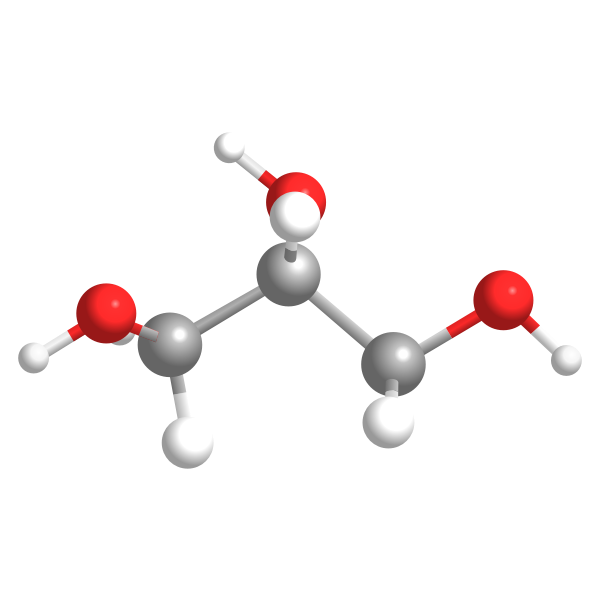
\includegraphics[width=0.35\linewidth]{Glycerol-molecule.png}
	\caption{Molecular structure of glycerol, highlighting the three hydroxyl groups responsible for hydrogen bonding.}
	\label{fig:glycerol_structure}
\end{figure}

At ambient pressure, glycerol exhibits a melting point of approximately 291~K, a boiling point near 563~K \cite{NIST_glycerol}, and a glass transition temperature $T_g \approx 190~\text{K}$ \cite[p.~6]{Angell1985}. The ability of glycerol to form multiple hydrogen bonds gives rise to a disordered network of competing local configurations and associated geometric frustration, which inhibits crystallization and makes it an excellent glass former and a model system for studying glassy dynamics.

As a hydrogen-bonding liquid, glycerol exhibits more complex behavior than simple van der Waals systems such as cumene discussed in \chap\nolinebreak \ref{chap:PCS}. In particular, the pressure dependence of fragility in hydrogen-bonded liquids has been a topic of significant interest over the past twenty-five years. Whereas most molecular liquids exhibit either decreasing fragility with increasing pressure or relatively weak pressure dependence, glycerol and similar hydrogen-bonded systems have been observed to show an increase in fragility at low to moderate pressures. This behavior is generally attributed to the influence of the hydrogen-bonding network under compression, whereas at sufficiently high pressures, where such bonding is strongly suppressed, one would expect a return toward dynamics more typical of simple van der Waals liquids \nolinebreak\cite{Casalini,Patkowski,Pronin}.

This chapter explores the current state of the literature on this topic and applies a new model to the dynamics of glycerol over a wide range of pressures and temperatures using literature data obtained through multiple experimental methods. In addition, $T_g(P)$ data, obtained \via the \tgp method described in \sect \ref{sec:IGPintro}, are used to constrain the analysis. The efficacy of viscosity data obtained by Cook \etal, which has come under some scrutiny, is reassessed, and the resulting thermodynamic scaling behavior is compared with previous literature results. Finally, a more precise measure of the pressure dependence of fragility in glycerol is presented.

\section{Earlier Works Regarding Glycerol Dynamics}

As previously asserted, glycerol is one of the most widely studied glass-forming systems, with the temperature dependence of its viscosity being investigated as far back as 1926 in the work of Tammann and Hesse \nolinebreak\cite{Tammann}.  However the modern history of glycerol, as relevant to this work, arguably begins with Davidson and Cole's investigation of the temperature dependence of the dielectric relaxation in glycerol circa 1951 \nolinebreak\cite{Davidson}.  Davidson and Cole found that not all associated liquids can be modeled with a simple single-relaxation or Debye equation as shown in \eqn\nolinebreak \ref{eqn:DebyeDielectric} \nolinebreak\cite{Debye}.  

\begin{equation}
\epsilon^*=\epsilon_\infty+\frac{\epsilon_0-\epsilon_\infty}{ 1+i\omega\tau_{0} },
\label{eqn:DebyeDielectric}
\end{equation}

 \noindent where $\epsilon_\infty$ and $\epsilon_0$ are the susceptibilities in the infinite-frequency and steady-state limits respectively.  Though 1-propanol was found to be well described by a simple Debye relationship, glycerol exhibited a higher degree of dispersion as vitrification accelerates and required unrealistically small values for its molecular volume in order for the observed relaxation time to conform to that predicted by the Debye hydrodynamic model for hard spheres.  Davidson and Cole correctly surmised that this was due to the existence of additional modes of relaxation available to glycerol that simply cannot exist for the simpler and more rigid 1-propanol molecule. To deal with this anomalous dielectric dispersion, Davidson and Cole suggested modeling such associated systems with the empirically derived "skewed" Debye like model 

\begin{equation}
\epsilon^*=\epsilon_\infty+\frac{\epsilon_0-\epsilon_\infty}{\left ( 1+i\omega\tau_{0} \right )^{\beta}},
\label{eqn:EmpiricalDielectric}
\end{equation}

\noindent where $\beta$ is the ''skewing parameter.'' Note that \eqn \ref{eqn:EmpiricalDielectric} reduces to \eqn \ref{eqn:DebyeDielectric} when $\beta=1$.  Starting with Cole and Cole, it became common in the literature of this time to plot the real \vs  imaginary components of this empirical expression as would have been common for the analysis of an analogous RC circuit\cite{Cole}. With regards to complex susceptibility, in the context of dielectric spectroscopy, the real part of \eqn \nolinebreak \ref{eqn:EmpiricalDielectric} corresponds to the non-dissipative component and the imaginary part to the dissipative component.  This can be modeled, for a simple Debye relaxation where $\beta=1$, in terms of a three component RC circuit as follows:

\begin{figure}[!htbp]
	\centering
	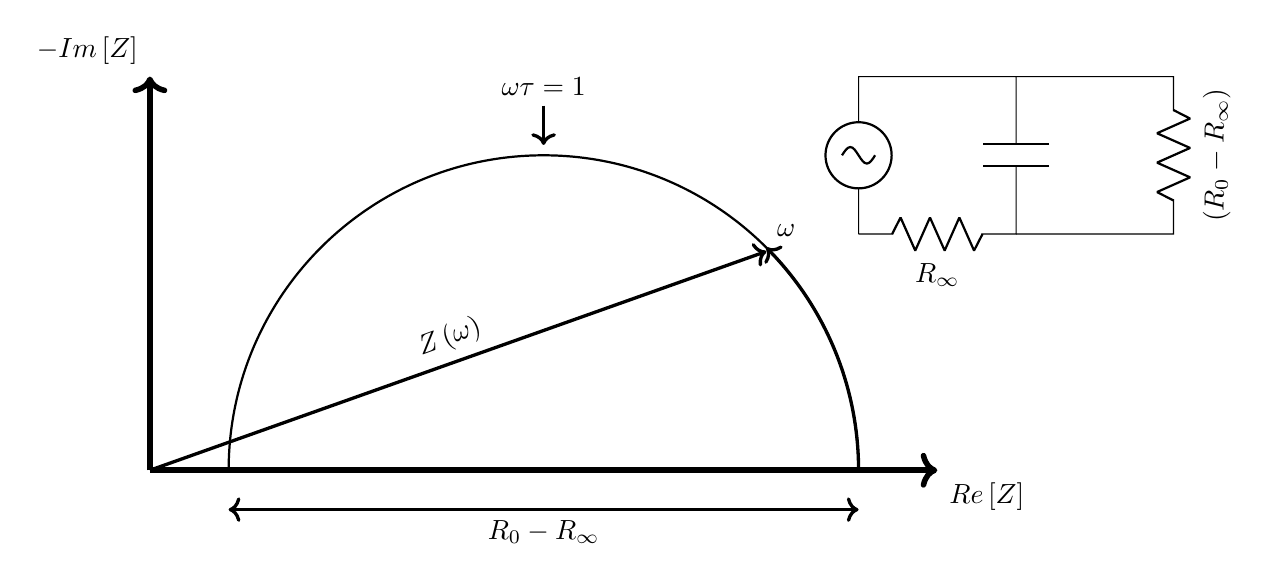
\begin{tikzpicture}
	
	\draw[->,line width=2pt] (0,0)--(10,0) node[anchor=north west] {$Re\left[Z\right]$} node[midway] (C) {};
	\draw[<->,very thick] (1,-.5)--(9,-.5) node[midway,anchor=north] {$R_0-R_\infty$};
	\draw[->,line width=2pt] (0,0)--(0,5) node[anchor=south east] {$-Im\left[Z\right]$};
	\draw[thick] (9,0) arc (0:180:4) node[midway] (A) {};
	\draw[->,very thick] (9,0) arc (0:45:4) node[anchor=south west] {$\omega$} node[anchor=west] (F) {};
	\node[above=0.5cm of A] (B) {$\omega\tau=1$};
	\draw[->,very thick] (B)--(A);
	\draw[->,very thick] (0,0)--(F) node[midway, anchor=south, rotate=20] {$Z\left(\omega\right)$};
	
	\draw (9,3) to[sinusoidal voltage source] (9,5) -- (11,5) to[C] (11,3) to[R](9,3);
	\draw (11,5) -- (13,5) to[R] (13,3) -- (11,3);
 	\draw (13.25,4) node[anchor=north,rotate=90]{$\left(R_0-R_\infty\right)$};
	\draw (10,2.75) node[anchor=north]{$R_\infty$};
		
	\end{tikzpicture}

	\caption{A system with a frequency dependent susceptibility and a single characteristic relaxation time $\tau$ driven at a given frequency $\omega$ can be modeled as an RC circuit as show here in the upper right corner. The complex impedance will be of the form $Z\left(\omega\right)=R_\infty+\frac{R_0-R_\infty}{1+i\omega\tau}$ which is functionally identical to the dielectric susceptibility of the simple Debye relaxation of \eqn\nolinebreak \ref{eqn:DebyeDielectric}.  Though the component which plays the role of irreversible dissipation is reversed in the case of the RC circuit above, both complex dielectric relaxation and this analogous electrical impedance will exhibit maximum dissipation at resonance where $\omega\tau=1$. }  
	\label{figure:ColeColePlot}
\end{figure}

\noindent Note that the magnitude of impedance will progress from $R_0$ to $R_\infty$ as the driving frequency is increased from $\omega=0$ to $\omega\rightarrow\infty$.  The impedance of the two limiting cases, $R_0$ and $R_\infty$, are analogous to the limiting values of the dielectric susceptibility $\epsilon_0$ and $\epsilon_\infty$ from \eqn\nolinebreak \ref{eqn:DebyeDielectric}, respectively. 

As previously mentioned, the Cole-Davidson model described by \eqn\nolinebreak \ref{eqn:EmpiricalDielectric} above may be described as a "skewed" Debye model when $0<\beta<1$ as it results in a distortion of the corresponding Cole-Cole plot.  An example of such a skewed plot of glycerol where $\beta=0.6$ and n-propanol where $\beta\approx1$, as obtained by Davidson, is shown below.  More importantly, Davidson provides a closed form expression for this distribution of simple Debye relaxations, first calculated by Fuoss and Kirkwood to describe dipole moments in polymers, which give rise to the Cole-Davidson model of \eqn\nolinebreak \ref{eqn:EmpiricalDielectric} and this is described in more detail in \chap\nolinebreak \ref{chap:PCS} \nolinebreak\cite{Fuoss}. For now, we assert that this skewing of the dielectric dispersion, increasing as the value of $\beta$ decreases, corresponds to a broader distribution of Debye-like relaxation processes.

\graphicspath{{Chapters/Glycerol/Figures/}}

\begin{figure}[!htbp]
	\begin{minipage}[t]{.45\textwidth}
	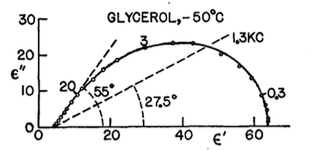
\includegraphics[width=\textwidth]{glycerolcole.png}
	\end{minipage}\hfill
	\begin{minipage}[t]{.1\textwidth}
	\end{minipage}\hfill
	\begin{minipage}[t]{.45\textwidth}
	\includegraphics[width=\textwidth]{nprop.png}
	\end{minipage}
	\caption{Cole-Cole plots of glycerol and n-propanol data (points).  Solid lines represent fits to the Cole-Davidson model of \eqn\nolinebreak \ref{eqn:EmpiricalDielectric} with beta-values of $0.6$ and $\approx 1$, respectively \protect\nolinebreak\cite{Davidson}.}  
	\label{figure:glcyerolcolecole}
	
\end{figure}

Davidson and Cole  also noted that the value of $\beta$ is essentially constant at ambient pressure over a temperature range from $40\;\si{\degreeCelsius}$ to $75\;\si{\degreeCelsius}$.  The implications of this being that the general structure of the distribution of relaxation modes is constant over a range of temperatures for which the dynamics of said relaxations are changing by at least six orders of magnitude.   Similar results have been found for many systems over the years and for such systems, this is known as time-temperature superposition.  More recently, the same has been found to hold over significant pressure ranges as well, in which case it is referred to as time-temperature-pressure superposition.  We found such results for Cumene, are described in \chap\nolinebreak \ref{chap:PCS}\textemdash$\beta$ being essentially constant over a wide range of temperature and pressure.

Though Davidson and Cole only considered the isobaric behavior of glycerol relaxation as a function of temperature, their contribution here provided some of the first data that could be used to estimate fragility\textemdash at least at atmospheric pressure. They demonstrated that the strong temperature dependence of glycerol relaxation is poorly described, even over this moderate temperature range, by a classical Arrhenius rate equation but was well fit, within experimental uncertainty, by the more empirical Vogel-Tammann-Fulcher (VTF) equation previously described by \eqn \ref{eqn:VTFintro} and first proposed by Tammann and Hesse to describe glycerol viscosity as a function of temperature \nolinebreak \cite{Tammann}.  Furthermore, they provided a closed form expression for the implied distribution of simple Debye relaxations underlying Cole-Davidson \eqn\nolinebreak \ref{eqn:EmpiricalDielectric} above.  Finally, they noted that the average molecular relaxation time of this distribution for glycerol would correspond to "hard-sphere" molecular dimensions, as provided by the classic Debye hydrodynamic theory, that are far too small to be physically realistic for glycerol, \eg, $1\times10^{-25}\;\si{\centi\meter\cubed}$, implying the existence of additional relaxation modes involving reorientation of molecular sub-units.  This observation was particularly significant, as it motivated the development and application of free-volume models for viscosity and structural relaxation upon which much of this chapter will rely.  Due to the importance of free-volume in this chapter and throughout the literature, particularly with regards to modeling viscosity of systems beyond ambient pressure, a discussion and derivation of the free-volume model will be provided in \sect\nolinebreak \ref{sec:freeVolume}.

Throughout the 1960s, work began to emerge within the literature probing viscosity and structural relaxation of glycerol beyond ambient pressure.  One of the first to appear was published in 1964 by McDuffie and Kelly where data for both viscosity, \via a rolling ball viscometer, and relaxation data, \via dielectric loss spectroscopy, were obtained \cite{McDuffie}. These methods were described previously in \sect \ref{sec:rolling_ball} and \sect \ref{sec:FRAintro}, respectively.  McDuffie and Kelly obtained viscosity data over three separate isotherms and dielectric relaxation data over a fourth which collectively covered a very small temperature range of $\Delta T=20 \;\si{\degreeCelsius}$, however, they extended these isotherms over what was, at the time, a very large range of pressure from ambient up to $4\;\si{\kilo\bar}$.  Beyond simply publishing some of the first high-pressure data for glycerol viscosity, McDuffie and Kelly's major contribution in this work was to show that neither the pressure nor temperature dependence of viscosity for glycerol was well described by the Eyring rate theory commonly used at the time and which will be described in the following section.  Also of considerable interest is that the free-volume model, described in \sect\nolinebreak \ref{sec:freeVolume}, was shown by McDuffie and Kelly to yield a compressibility for glycerol that is not congruent with high-pressure values derived from ultrasonic probes. They showed that the implementation of pressure-independent thermal expansion coefficients within the free-volume model leads to an overestimation of the pressure dependence of viscosity.  However these discrepancies were quickly addressed the following year, in 1966, by Matheson \nolinebreak\cite{Matheson}.  His arguably obvious approach was simply to apply a quadratic model to account for the pressure dependence of $\nu_{m}$ in the free-volume expression (\eqn\nolinebreak \ref{eqn:expandedViscosity}) from \sect\nolinebreak \ref{sec:freeVolumederive}.  An identical approach was used to describe the temperature dependence of several other liquids; however, the limited temperature range in McDuffie and Kelly's data was insufficient to meaningfully constrain a quadratic temperature dependence of $\nu_{m}$ in glycerol.  Still, in effectively addressing the shortcomings of early free-volume models exposed by McDufffie and Kelly \via extending the model beyond ambient pressure, Matheson's contribution was very significant. What Matheson was in want of, and what was conspicuously lacking in the literature up to this point, would be carefully collected data for glycerol viscosity or structural relaxation spanning a large temperature and pressure range.

This data gap was quickly filled by Johari and Whalley in the early 1970s with the publication of a highly cited study reporting dielectric susceptibility measurements of glycerol spanning a dynamic range of six decades \nolinebreak\cite{JohariWhalley}. Notably, their measurements extend to pressures as high as $53\;\si{\kilo\bar}$, comparable to those accessible in modern diamond anvil cell experiments, making this work a rare early example of high-pressure glassy dynamics measurements at such extremes. Their data also span a significantly broader range of temperature and pressure than previous studies, from ambient conditions to $53\;\si{\kilo\bar}$ and $-55\;\si{\degreeCelsius}$ to $84\;\si{\degreeCelsius}$, respectively.

At lower temperatures, Johari and Whalley were able to probe the relaxation dynamics of glycerol very near the glass transition. At higher temperatures, above $T = 250\;\si{\kelvin}$, their data fall approximately three decades short of approaching the glass transition. Nevertheless, the overall quality of the data has proven to be exceptional, enabling investigations into the pressure dependence of parameters such as $\beta$, defined in \eqn\nolinebreak \ref{eqn:EmpiricalDielectric}, and, later, fragility.

While the extent of their pressure range is remarkable, the accuracy of the data at the highest pressures was difficult to assess given the experimental limitations of high-pressure techniques available at the time. In this context, the incorporation of $T_g(P)$ data from the literature through the \tgp method developed in our laboratory provides a means to assess the consistency of these high-pressure measurements within a unified thermodynamic framework. As such, this work has served as a foundational reference for subsequent studies of glycerol and other glass-forming systems, with numerous citations in the literature, including those examining the pressure dependence of fragility \nolinebreak\cite{Johari2,Paluch,Forsman,Pawlus}.

Around a decade later, in 1986, Forsman \etal published a paper also probing dielectric relaxation of glycerol up to pressures of 10~kbar \nolinebreak \cite{Forsman}.  They had the advantage of nearly a decade of advancement in instrumentation and thus were able to probe significantly faster relaxations, up to $13\;\si{\mega\hertz}$.  However, these works provided relatively limited additional data, and the accessible pressure and temperature ranges were already largely covered by the earlier measurements of Johari and Whalley. While extending to faster relaxation times, such data do not substantially enhance subsequent analyses of fragility following its formal introduction by Angell, which are primarily governed by behavior near the glass transition. Though Forsman was focused more on the broadening of the loss peak as a function of pressure and furthers the discussion of many-body relaxation theory to account for deviations of the loss spectra from Debye theory, this work is worthy of mention here as it references several other papers providing data for glycerol relaxation collected over several decades.

Another work worthy of mention would be the work published by Demoulin in the early 70's \nolinebreak\cite{Demoulin}.  Though data was only taken at ambient pressure and low temperatures, Demoulin probed glycerol relaxations directly in the time domain \via photon correlation spectroscopy as described in \sect\nolinebreak \ref{sec:PCSintro}.  Though his data was confined to a relatively limited dynamic range, as autocorrelators of this era were among the first and significantly slower than those currently commercially available, with the aid of ultrasonic measurements a reasonable dynamic range was obtained.  The aim of Demoulin was not to extend the dynamic range of data available for glycerol relaxation, but rather to prove the efficacy of digital photon correlation spectroscopy as a probe of relaxation dynamics over what was an exceedingly large dynamic range for the time.  In \chap\nolinebreak \ref{chap:PCS}, a method for extending this probe into the range of very high pressures will be presented.  It is interesting here to note that, though the data obtained \via photon correlation spectroscopy is in the time domain, the Cole-Davidson distribution, being used pervasively throughout the literature to describe the dynamics of structural relaxation probed \via dielectric spectroscopy and ultrasonics methods, is most naturally expressed in terms of frequency.  This work was published before that of Lindsey and Patterson, which worked out a simple means of translating between the Williams-Watts distribution, expressed most naturally in the time domain and commonly used to model data obtained \via photon correlation spectroscopy, and the Cole-Davidson distribution of \eqn\nolinebreak \ref{eqn:EmpiricalDielectric} \nolinebreak\cite{Lindsey}.  Thus it is not surprising that Demoulin chose to impart significant effort to fit his time-domain data to the more common, yet inconvenient, Cole-Davidson distribution so that it may be directly compared to data within the literature.  His method for accomplishing this will be extended in  \chap \nolinebreak\ref{chap:PCS}, taking advantage of modern computational tools, for exactly the same reasons.

Demoulin's method of PCS will later be well established to constitute a direct measurement of structural $\alpha$-relaxation within a glass-forming system.  However, another direct probe, this time of viscosity, was introduced in the late 1970s by Geils and Keezer \nolinebreak\cite{Geils}.  The rolling ball viscometer as a means of directly measuring viscosity \via tracking the terminal velocity of a metal ball rolling down an incline, as previously described in \sect \nolinebreak\ref{sec:rolling_ball}, certainly predated the work of Geils and Keezer, however early implementations placed great restrictions on the geometry of the viscometer requiring that the ratio of the rolling ball diameter to that of the viscometer remain in one or the other limiting extremes\textemdash either rolling without slipping down a surface of the viscometer or lacking any significant interaction with the confining surfaces \nolinebreak\cite{Sutterby,Hubbard}.  Geils and Keezer worked out the means of accounting for the correction factors associated with wall effects for this method, allowing for greater flexibility in experimental design to allow for temperature and potentially pressure control, drastically increasing its efficacy as a probe for viscosity of glass-forming systems.  

\section{Reduction of extrapolation error in fragility measurements from pressure-limited data \via implementation of \tgp}

	Viscosity measurements at elevated pressure for glycerol up to about $4\;\si{\kilo\bar}$, first obtained by McDuffie and Kelly, was reported in the Journal of Chemical Physics in 1964 \nolinebreak\cite{McDuffie}.  This pressure range was significantly extended by just under an order of magnitude \via the work of Cook \etal in 1993 and 1994 implementing a diamond anvil cell viscometer attached to a centrifuge \nolinebreak\cite{Cook,Cook2}.  The data of Cook \etal were then used to investigate the pressure dependence of fragility  over this domain and appeared to show a trend of steadily increasing fragility from approximately $m\approx 55$ ($m^*=3.2$) at ambient pressure up to $m\approx 170$ ($m^*=13.6$) at $3\;\si{\giga\pascal}$ as shown in \fig \nolinebreak \ref{figure:CookFrag}.
	
	\pgfplotsset{table/search path={Chapters/glycerol/Figures},}
	\begin{figure}
		\centering
		\resizebox{0.85\textwidth}{!}{%
			\begin{minipage}[t]{.46\textwidth}
				\centering
				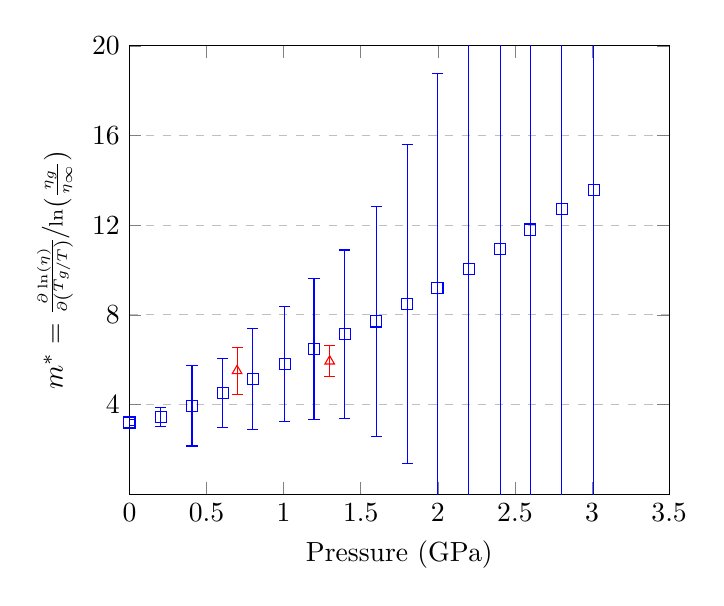
\begin{tikzpicture} 
					\begin{axis}[
						ylabel={$m^*=\nicefrac{\frac{\partial \ln(\eta) }{\partial \left(\nicefrac{T_g}{T}\right)}}{\ln\left( \frac{\eta_g}{ \eta_\infty}\right )}$},
						xlabel={Pressure ($\si{\giga\pascal}$)},
						xmin=0, xmax=3.5,
						ymin=0, ymax=20,
						xtick={0,.5,1,1.5,2,2.5,3,3.5},
						ytick={4,8,12,16,20},
						ymajorgrids=true,
						grid style=dashed,
						]
						\addplot+[only marks, mark=square,error bars/.cd, y dir=both,y explicit]
						coordinates { 
							(0,3.195) +- (0,.132) 
							(.202077,3.445) +- (0,.435) 
							(.405465,3.945) +- (0,1.8) 
							(.605676,4.521) +- (0,1.53) 
							(.79953,5.144) +- (0,2.256)
							(1.006097,5.8055) +- (0,2.576)
							(1.196773,6.467) +- (0,3.157)
							(1.396984,7.1272) +- (0,3.7655)
							(1.600372,7.7049) +- (0,5.129)
							(1.800583,8.468) +- (0,7.1188)
							(1.997615,9.207) +- (0,9.5487)
							(2.201004,10.048) +- (0,12.786)
							(2.404392,10.937) +- (0,17.356)
							(2.598247,11.802) +- (0,22.653)
							(2.804813,12.714) +- (0,29.424)
							(3.01138,13.569) +- (0,36.895)
						};
						\addplot+[red, only marks, mark=triangle,error bars/.cd, y dir=both,y explicit]
						coordinates {
							(.697836,5.499) +- (0,1.04) 
							(1.298467,5.927) +- (0,.6921)
						};
					\end{axis} 
				\end{tikzpicture}
			\end{minipage}
			\hspace{0.04\textwidth}
			\begin{minipage}[t]{.46\textwidth}
				\centering
				\begin{tikzpicture} 
					\begin{axis}[
						ylabel={$\nicefrac{\ln\left(\frac{\eta}{\eta_\infty}\right)} {\ln\left(\frac{\eta_g}{\eta_\infty}\right)}$},
						xlabel={Temperature ($\nicefrac{T_g}{T}$)},
						xmin=0, xmax=1,
						ymin=0, ymax=1,
						xtick={0,0.2,0.4,0.6,0.8,1},
						ytick={0.2,0.4,0.6,0.8,1},
						ymajorgrids=false,
						grid style=dashed,
						legend style={at={(0.325,.95)}},
						]
						
						\draw[dashed,thick] (0,0)--(1,1);
						\draw[dashed, thick] plot [smooth] coordinates {(0,0) (.1,.00722) (.2,.01609) (.3,.02727) (.4,.04179) (.5,.0614) (.6,.08936) (.7,.13243) (.8,.20741) (.9,.37059) (.95,.55417) (1,1)};
						\node[rotate=43.5] at (0.45,.5) {Strong};
						\node[rotate=10] at (0.3,.075) {Fragile};
						
						\addplot table [only marks,x=a, y=b, col sep=comma] {0GPAglycerol.csv};
						\addlegendentry{{\scriptsize 0.0 \;\si{\giga\pascal}}}
						\addplot table [only marks,x=a, y=b, col sep=comma] {04GPAglycerol.csv};
						\addlegendentry{{\scriptsize 0.4 \;\si{\giga\pascal}}}
						\addplot table [only marks,x=a, y=b, col sep=comma] {13GPAglycerol.csv};
						\addlegendentry{{\scriptsize 1.3 \;\si{\giga\pascal}}}
						\addplot table [only marks,x=a, y=b, col sep=comma] {3GPAglycerol.csv};
						\addlegendentry{{\scriptsize 3.0 \;\si{\giga\pascal}}}
						
					\end{axis} 
				\end{tikzpicture}
			\end{minipage}%
		}
		
		\caption{Left: the calculations of Cook \etal for the isobaric fragility of glycerol as a function of pressure with the glass transition defined at $10^{15}$ centipoise. Note that these values have been scaled to reflect our redefinition of fragility as defined in \eqn\nolinebreak\ref{eqn:scaledfragility}. This scaling of fragility is trivially accomplished as Cook \etal conveniently provides their fit parameters. The more precise values ({\color{red}$\triangle$}) were obtained from pseudoisobaric data runs of Cook \etal. Right: Angell plots for Cook \etal's 0.4, 1.3, and 3.0 \si{\giga\pascal} pseudoisobars \protect\nolinebreak\cite{Cook2}. The 0.0 \si{\giga\pascal} isobar data is from Laughlin's 1969 Ph.D. thesis \protect\nolinebreak\cite{Laughlin} although all values plotted here were directly extracted from Cook \etal's published figures.}
		\label{figure:CookFrag}
	\end{figure}  
	
	\noindent Note that, though the definition of fragility provided by \eqn\nolinebreak \ref{eqn:scaledfragility}  is arguably more physically meaningful, it may be convenient for the sake of literature comparisons to express some fragilities in terms of the more classical definition of \eqn\nolinebreak \ref{eqn:fragility}.  Thus to alleviate any confusion we will adopt a consistent notation of $m$ and $m^*$ to indicate the classical fragility of \eqn\nolinebreak \ref{eqn:fragility} and the scaled fragility of \eqn\nolinebreak \ref{eqn:scaledfragility}, respectively.  Returning now to \fig \nolinebreak \ref{figure:CookFrag}, note the excessive error associated with these fragility calculations arising from the necessity to extrapolate the VTF model over several orders of magnitude up to the glass transition.  The fact that this trend towards extreme fragility is not in satisfactory agreement with subsequent publications, particularly at elevated pressures, and the excessive error implying that the fragility measurements at high-pressure are essentially meaningless has led to the Cook \etal data being generally under-emphasized.  Paluch \etal drew attention to these concerns as well as the fact that several of the viscosity measurements were made near the melt temperature, $T_m$, where VTF model extrapolations are known to be unreliable \nolinebreak\cite{Paluch}.  The fundamental limitation for Cook \etal was that rolling ball viscometry, even when implemented within a centrifuge, can only measure viscosities up to on the order of $10^9cP$\textemdash \ie, as much as six orders of magnitude away from the glass transition at which fragility is assessed.  The data of Cook \etal, even with these concerns, does show strong support for an increasing trend in fragility with pressure up to around $2\;\si{\giga\pascal}$, which is not unexpected for a hydrogen bonding liquid where increasing fragility can be explained as arising from the diminished free-volume inhibiting hydrogen bonding.  Beyond approximately $2\;\si{\giga\pascal}$, the uncertainties in these fragilities obtained from propagating the errors in the fit parameters of the VTF equation seems to render the actual values of fragility statistically meaningless. Though the assessment of Cook \textit{et al.}, that the fragility continues to increase with pressure beyond this point, may have been somewhat compelling—given that the measurements follow a well-defined linear regression and that their standard Angell plots (shown here as modified Angell plots on the right side of \fig~4.4) appear to exhibit increasing curvature with pressure—the higher-pressure data are dubious, to say the least. Not only are the associated uncertainties excessive, but by $P = 3.0\;\si{\giga\pascal}$ glycerol has already reached a fragility of $m \approx 170$ ($m^* = 13.6$), \ie, near the upper limit of fragility observed in glass-forming liquids.  This linear trend in fragility certainly cannot continue indefinitely yet, at a pressure of $3\;\si{\giga\pascal}$, there is no indication of departing from said trend. 
	
	\pgfplotsset{table/search path={Chapters/Glycerol/SupportingFiles},}
	\begin{figure}[!htbp]
		\centering
		\begin{minipage}[t]{.45\textwidth}
			\centering
			\begin{tikzpicture} 
				\begin{axis}[
					samples=100,
					title={\parbox{\textwidth}{\centering\small $1.3\;\si{\giga\pascal}$ Scaled Angell Plot}},
					width=\linewidth,
					ylabel={$\nicefrac{\log\left(\frac{\eta}{\eta_\infty}\right)} {\log\left(\frac{\eta_g}{\eta_\infty}\right)}$},
					xlabel={Temperature $\left(\nicefrac{T_g}{T}\right)$},
					xmin=0, xmax=1.1,
					ymin=0, ymax=1.1,
					xtick={.2,.4,.6,.8,1},
					ytick={0,.2,.4,.6,.8,1},
					ymajorgrids=true,
					grid style=dashed,
					legend style={at={(0,1)},nodes={scale=.75,transform shape}, anchor=north west}
					]
					
					\addplot expression[domain=0:1.1, very thick, dashed,mark=none, Green] {.0554175*((-7.011+19.05*156.29/(227.81/x-156.29))/2.302585+3.044838613)};
					\addlegendentry{{\scriptsize \tgp}};
					\addplot expression[domain=0:1.1, very thick, solid,mark=none, Green] {.0641*((-1.378+6.629*206.496/(244.61/x-206.496))/2.302585+0.5984578)};
					\addlegendentry{{\scriptsize w/o \tgp}};
					
					\addplot [only marks, mark options={color=Green}] table [x=xmod, y=ymod, col sep=comma] {CookSystemicMissPlots.csv};
					\addplot [only marks, mark options={color=Green,fill=white}] table [x=xmodtgp, y=ymodtgp, col sep=comma] {CookSystemicMissPlots.csv};
					
				\end{axis} 
			\end{tikzpicture}
		\end{minipage}\hfill
		\begin{minipage}[t]{.05\textwidth}
		\end{minipage}\hfill
		\begin{minipage}[t]{.45\textwidth}
			\centering
			\begin{tikzpicture}
				\begin{axis}[
					samples=100,
					title={\parbox{\textwidth}{\centering\small Systemic Error in \tgp Extrapolations}},
					width=\linewidth,
					ylabel={$\log_{10}(\eta)$ (cP)},
					xlabel={Temperature ($\si{\kelvin}$)},
					xmin=150, xmax=400,
					ymin=0, ymax=18,
					xtick={200,300,400},
					ytick={0,2,4,6,8,10,12,14,16,18},
					ymajorgrids=true,
					grid style=dashed,
					unbounded coords=discard,
					legend style={at={(1,1)},nodes={scale=.75,transform shape}, anchor=north east}
					]
					
					\addplot [only marks, mark options={color=Red}] table [x=x0GPA, y=y0GPA, col sep=comma] {CookSystemicMissPlotsLog.csv};
					\addlegendentry{{\scriptsize $0.0\;\si{\giga\pascal}$}};
					
					\addplot [only marks, mark options={color=Orange},mark=diamond*] table [x=x025GPA, y=y025GPA, col sep=comma] {CookSystemicMissPlotsLog.csv};
					\addlegendentry{{\scriptsize $.25\;\si{\giga\pascal}$}}
					
					\addplot [only marks, mark options={color=YellowOrange},mark=triangle*] table [x=x07GPA, y=y07GPA, col sep=comma] {CookSystemicMissPlotsLog.csv};
					\addlegendentry{{\scriptsize $.70\;\si{\giga\pascal}$}}
					
					\addplot [only marks, mark options={color=YellowGreen},mark=square*] table [x=x1GPA, y=y1GPA, col sep=comma] {CookSystemicMissPlotsLog.csv};
					\addlegendentry{{\scriptsize $1.0\;\si{\giga\pascal}$}}
					
					\addplot [only marks, mark options={color=Green}] table [x=x13GPA, y=y13GPA, col sep=comma] {CookSystemicMissPlotsLog.csv};
					\addlegendentry{{\scriptsize $1.3\;\si{\giga\pascal}$}}
					
					\addplot  [only marks, mark options={color=BlueGreen},mark=diamond*] table [x=x17GPA, y=y17GPA, col sep=comma] {CookSystemicMissPlotsLog.csv};
					\addlegendentry{{\scriptsize $1.7\;\si{\giga\pascal}$}}
					
					\addplot [only marks, mark options={color=Blue},mark=triangle*] table [x=x25GPA, y=y25GPA, col sep=comma] {CookSystemicMissPlotsLog.csv};
					\addlegendentry{{\scriptsize $2.5\;\si{\giga\pascal}$}}
					
					\addplot [only marks, mark options={color=Violet},mark=square*] table [x=x3GPA, y=y3GPA, col sep=comma] {CookSystemicMissPlotsLog.csv};
					\addlegendentry{{\scriptsize $3.0\;\si{\giga\pascal}$}}
					
					\addplot expression[domain=150:400, very thick, solid,mark=none, Red] {(-6.143+18.012*124.904/(x-124.904))/2.302585093}; %0 GPa
					\addplot expression[domain=150:400, very thick, solid,mark=none, Orange] {(-5.625+16.574*136.265/(x-136.265))/2.302585093}; %0.25 GPa
					\addplot expression[domain=200:400, very thick, solid,mark=none, YellowOrange] {(-3.908+10.987*170.013/(x-170.013))/2.302585093}; %0.7 GPa
					\addplot expression[domain=200:400, very thick, solid,mark=none, YellowGreen] {(-2.623+8.38*190.157/(x-190.157))/2.302585093}; %1 GPa
					\addplot expression[domain=210:400, very thick, solid,mark=none, Green] {(-1.378+6.629*206.496/(x-206.496))/2.302585093}; %1.3 GPa
					\addplot expression[domain=230:400, very thick, solid,mark=none, BlueGreen] {(0.167+5.136*223.088/(x-223.088))/2.302585093}; %1.7 GPa
					\addplot expression[domain=250:400, very thick, solid,mark=none, Blue] {(2.867+3.619*244.082/(x-244.082))/2.302585093}; %2.5 GPa
					\addplot expression[domain=255:400, very thick, solid,mark=none, Violet] {(4.348+3.151*252.212/(x-252.212))/2.302585093}; %3 GPa
					
				\end{axis} 
			\end{tikzpicture}
		\end{minipage}\hfill
		
		\caption{Left:  A scaled Angell plot of the data of Cook \etal clearly demonstrates the over-estimation of fragility occurring at $1.3\;\si{\giga\pascal}$ due to extreme extrapolation up to the glass transition that is rectified \via the inclusion of \tgp data.  The same data is provided for both the solid and dotted VTF fits\textemdash scaled accordingly to their fit parameters and the glass transition temperatures they predict.  Right: Isobaric data from Cook \etal showing the general trend of under-estimation followed by increasing over-estimation of the glass transition temperature with increasing pressure.  The \tgp method provides the isochronal data at the glass transition \protect\nolinebreak\cite{Cook2}.}\label{figure:CookMiss}
		
	\end{figure}
	
	Furthermore, it is worth noting that the $3\;\si{\giga\pascal}$ fragility shown in \fig \nolinebreak \ref{figure:CookFrag} is based on only four data points and, though it is less evident in our modified Angell plot than it would be in a classical Angell plot, it does not converge to a similar infinite temperature viscosity as do data obtained at lower pressures. It is therefore not surprising that this data might yield an excessively high fragility while having error bars that include negative values of fragility\textemdash statistically speaking this is a meaningless extrapolation.  In truth, this point should likely have been omitted from Cook \etal's analysis as it relies on only three reasonably reliable data points\textemdash the underlying data for these extrapolations are shown explicitly in \fig \nolinebreak \ref{figure:CookMiss} (right), where the limited temperature coverage of the isobaric reconstructions becomes apparent.  The $50.0\;\si{\degreeCelsius}$ data point requiring a free-volume model extrapolation of almost $1\;\si{\giga\pascal}$.  However omitting the $50.0\;\si{\degreeCelsius}$ data point would leave only the $22.5$, $75.0$, and $125.0\;\si{\degreeCelsius}$, two of which still require slight extrapolation to $3\;\si{\giga\pascal}$, and require one to perform a non-linear model fit with only three data points providing constraint to a three parameter VTF model\textemdash though technically possible, an arguably meaningless endeavor.  This was the root cause of their rapidly increasing fragility estimates\textemdash simply a lack of data to properly constrain the VTF model fits and extreme extrapolation over orders of magnitude as none of this data is within the vicinity of the glass transition.

	More recent work has made a well supported case that the fragility of glycerol increases with pressure due to a progressive inhibiting of hydrogen bonding up to approximately $2\;\si{\giga\pascal}$ at which point it levels off becoming relatively constant.  It would be reasonable to assert that Cook \etal's data, as analyzed here with further constraints using data from our lab, equally well supports this general trend of fragility.  Arguably, the analysis supports a general increasing trend in fragility as pressure increases up to approximately $2\;\si{\giga\pascal}$ even if little confidence can be put into the exact fragility values above the point that the error begins to diverge rapidly.  Beyond $2\;\si{\giga\pascal}$ little can be confidently asserted from Cook \etal's analysis however it does not contradict a constant fragility when the propagated errors are accounted for.  
	
	In order to assess the validity of Cook \etal's high-pressure data and the associated fragility, it is necessary to diminish these large error bars.  This can be accomplished by addressing one of their two primary underlying issues\textemdash extreme data extrapolation.  The \tgp process developed by our group provides a direct measurement of the glass transition as a function of pressure allowing for a re-analysis of the Cook \etal data without the need for extrapolation of the VTF model over so many orders of magnitude.  This \tgp data is provided in \app\nolinebreak \ref{app:CumeneIGP} (\tbl\nolinebreak \ref{table:IGPdataGlycerol}) along with the associated Andersson-Andersson regression fit \cite{Andersson}.  Using these values for the glass transition pressure on any given isotherm and assuming this transition to occur on an isochronal curve associated with a viscosity of $\eta=10^{15}~cP$, the data Cook \etal were refit to a classical VTF model. 	
	
	\begin{figure}[!htbp]
		\centering
		\begin{tikzpicture}
			\begin{axis}[
				width=0.82\textwidth,
				height=0.55\textwidth,
				xlabel={Pressure (\si{\giga\pascal})},
				ylabel={$T_g$ (P)},
				xmin=0.15,
				xmax=4.60,
				ymin=145,
				ymax=440,
				xtick={0.5,1.0,1.5,2.0,2.5,3.0,3.5,4.0,4.5},
				ytick={150,200,250,300,350,400,450},
				ymajorgrids=true,
				xmajorgrids=true,
				grid style=dashed,
				legend style={
					at={(0.03,0.97)},
					anchor=north west,
					draw=none,
					fill=none
				},
				tick label style={font=\small},
				label style={font=\small},
				]
				
				% Cumene IGP data points
				\addplot[
				only marks,
				mark=*,
				mark size=2.4pt
				]
				table[
				col sep=comma,
				x index=0,
				y index=1
				]{Chapters/Back_matter/Figures/CumeneTGPdata.csv};
				\addlegendentry{\tgp data}
				
				% Andersson--Andersson fit
				\addplot[
				domain=0.198:4.55,
				samples=300,
				thick
				]
				{131.145*(1 + 1.64181*x/1.21852)^(1/1.64181)};
				\addlegendentry{Andersson--Andersson fit}
				
			\end{axis}
		\end{tikzpicture}
		\caption{Cumene glass-transition temperatures obtained from \tgp measurements as a function of pressure. Points correspond to the appendix data (\app\ref{app:CumeneIGP}) were one may also find the associated Andersson--Andersson fit. It should be emphasized that the $T_g(P)$ isochrone shown here does not correspond to the conventional definition of the glass transition at $\tau_g = 100~\si{\second}$, but is instead associated with a characteristic relaxation time for this specific \tgp data that will be shown to be approximately $\tau \approx 220~\si{\second}$.}
		\label{fig:CumeneIGPAA}
	\end{figure} 
	
	Note that most of the data of Cook \etal were obtained over isotherms at varying pressures.  In order to calculate fragility, they fit five sets of isothermal viscosity data to the classic free-volume model of \eqn\nolinebreak \ref{eqn:logViscosity}.  The Tait equation of state, fit to density data provided by Bridgman \nolinebreak\cite{BridgmanGly}, was implemented to convert pressure to volume.  More details regarding the implementation of the Tait equation of state for glycerol are provided in \app\nolinebreak \ref{app:GlycerolEOS} as Cook \etal and this work use this free-volume model to obtain (mostly) interpolated isobaric data as true isobaric data is difficult to obtain experimentally given that pressures will vary significantly within the DAC under thermal expansion.  Thus it is this interpolated isobaric data that is used in the fits to the VTF model for fragility analysis. 
	
	\fig \nolinebreak \ref{figure:CookMiss} (left) provides a scaled Angell plot both excluding the \tgp glass transition point (solid) as well as the refit passing through the \tgp point (dashed) for a $1.3\;\si{\giga\pascal}$ isobar.  Note that the lower five data points associated with both the dashed and solid regressions are in fact the same data from Cook \etal\textemdash scaled according to their associated VTF fits and glass transition temperatures.  The \tgp point is also provided and is, on a scaled Angell plot, located at (1,1) by definition.  It is immediately clear that both adequately describe Cook \etal's data however omitting the \tgp data leads to a significant over-estimation of fragility.  This is associated with an over-estimation of the glass transition temperature.  \fig \nolinebreak\ref{figure:CookMiss} (right) shows eight isobaric data sets, consisting of four to five data points each, ranging left to right from $0\;\si{\giga\pascal}$ to $3\;\si{\giga\pascal}$ which are obtained from the aforementioned free-volume fits to Cook \etal's published isothermal data.  The VTF fits to this data exclude the \tgp point and thus help to demonstrate the error that arises from the extrapolation of the VTF equation.  Notice that at the lowest pressures (left most curves) there is a systematic under-estimation of the glass transition temperature due to model extrapolation.  However, as we move up in pressure (to the right of the figure) we begin to increasingly over-estimate the glass transition temperature and thus over-estimate the fragility.  This trend is what is giving rise to Cook \etal's exploding fragility measurements.

From this reassessment of the data of Cook \etal, we see a very different behavior of fragility as a function of pressure.  Though, as demonstrated in \fig \nolinebreak \ref{figure:CookProninReiser}, the calculations of fragility attained from the Cook \etal data connected \via our \tgp isochronal data were still not found to be in agreement with more recent measurements, the general trend is found to be somewhat congruent \nolinebreak\cite{Pronin,Reiser}.  It should be noted that the actual values of fragility, apart from their trend with pressure, are somewhat dependent on the viscosity at the glass transition.  Following standard practice, we let the Tg(P) transition correlate with a viscosity of $\approx 10^{15}cP$.  

\pgfplotsset{table/search path={Chapters/Glycerol/Figures},}
\begin{figure}[!htbp]
	\centering
	
	\begin{tikzpicture} 
		\begin{axis}[
			samples=100,
			title={\parbox{0.35\textwidth}{\centering Isothermal Glycerol Fragilities With Increasing Pressure}},
			width=\linewidth,
			height=10cm,
			xmin=0, xmax=5,
			ymin=40, ymax=90,
			xtick={0,1,2,3,4,5},
			ytick={40,50,60,70,80,90},
			ztick={5,10,15},
			ylabel style = {align=center},
			ylabel={Pronin/Reiser \etal Fragility $m_t$},
			ymajorgrids=true,
			grid style=dashed,
			legend style={at={(1,0)},anchor=south east}
			]
			
			\addplot [blue, only marks, mark=square,error bars/.cd, y dir=both,y explicit] table [x=xcook, y=ycook, y error plus=maxcook, y error minus=mincook, col sep=comma] {FragilityComparison.csv};
			\addlegendentry{{\scriptsize Cook \etal \cite{Cook2}}}
			
			\draw[black,dashed, thick] (2,40)--(2,90);
			\draw[black,dashed, thick] (3,40)--(3,90);
			\draw[black,very thick, ->] (2.85,55)--(3,55);
			\draw[black,very thick, ->] (2.15,55)--(2,55);
			\node[] at (2.5,55) {\parbox{0.15\textwidth}{\centering H-Bonding Suppression}};
			
			\addplot+[red,only marks, mark=triangle,error bars/.cd, y dir=both,y explicit]
			coordinates { 
				(0,50.72324)    +- (0,1.938) 
				(1.426686,63.16297)    +- (0,3.0665)
				(2.170432,71.81292)    +- (0,5.063)  
				(2.464173,71.4947)    +- (0,4.918) 
				(2.966801,70.25072)    +- (0,2.95)
				(2.966979,69.1514)    +- (0,2.95)
				(3.599749,73.63549)    +- (0,3.0087) 
				(4.002432,75.05304)    +- (0,2.89296) 
				(4.468517,74.64802)    +- (0,6.914) 
				(4.54875,73.80906)    +- (0,7.985)      
			};
			\addlegendentry{{\scriptsize Pronin \cite{Pronin}}}
			
			\addplot+[green,only marks, mark=star,error bars/.cd, y dir=both,y explicit]
			coordinates { 
				(0,53.03688)    +- (0,3) 
				(.1,52.32513)    +- (0,3)
				(.2,53.18672)    +- (0,3)  
				(.3,53.13989)    +- (0,3) 
				(.4,54.01085)    +- (0,3)
				(.5,55.05975)    +- (0,3)
				(.6,56.05246)    +- (0,3) 
				(.7,57.07326)    +- (0,3)        
			};
			\addlegendentry{{\scriptsize Reiser \etal \cite{Reiser}}}
			
			\addplot+[no marks,very thick, black] {46.664493+27.40865/(1+4.496047*e^(-1.40425*x))};
			\addlegendentry{{\scriptsize Guide}}
			
			\addplot+[no marks,very thick, dashed, black] {0.43429*(38.964-.299834*(x*10))*(1+(38.964-.299834*(x*10))/(19.0451-.625929*(x*10)+.00644846*(x*10)^2-.00000616589*(x*10)^3))};
			\addlegendentry{{\scriptsize Surface}}
			
		\end{axis} 
	\end{tikzpicture}
	
	\caption{The fragility measurements calculated from classic VTF fits to Cook \etal's viscosity data corrected \via the inclusion of our \tgp glass transition point ($\color{blue}\square$) are shown above to be no longer wholly incongruent with more recent work. A smooth curve is included as a guide to the eye through the Pronin ($\color{red}\triangle$) and Reiser \etal ($\color{green}\star$) data, suggesting that the increase in fragility appears to saturate between 2 and 3 $\si{\giga\pascal}$ as originally asserted by Paluch \protect\nolinebreak\cite{Paluch} and Pawlus \protect\nolinebreak\cite{Pawlus}. The fragilities of Cook \etal retain relatively large uncertainties, thus cannot reflect accurately the fine behavior of fragility as a function of pressure, yet do seem to reflect this fragility increase between 2 and 3 $\si{\giga\pascal}$. A reasonable trend-line is provided that falls within all error bars.} 
	\label{figure:CookProninReiser}
\end{figure}

A quick assessment of \fig \nolinebreak \ref{figure:CookFragIGP} might suggest a decrease in fragility from ambient pressure up to approximately $1.5\;\si{\giga\pascal}$, and the propagated uncertainties derived from the covariance of the VTF fit parameters appear to indicate statistical significance in this trend. However, these error bars reflect only the internal consistency of the VTF fitting procedure and do not account for more fundamental sources of uncertainty.

In this regime, the determination of fragility relies on extrapolation of the VTF form over many decades in relaxation time, with minimal experimental constraint near the glass transition. While the inclusion of the \tgp isochron constrains the location of $T_g$, it provides only a single point in the vicinity of the transition and therefore does not meaningfully constrain the slope of the VTF function from which the fragility is derived. As a result, the calculated fragility remains strongly dependent on both the assumed validity of the VTF form and the underlying Cook \etal\ dataset. Consequently, the apparent decrease in fragility should not be interpreted as physically robust. Rather, it reflects the limitations of the available data and fitting procedure, which are insufficient to reliably capture the evolution of fragility.

\pgfplotsset{table/search path={Chapters/glycerol/Figures},}
\begin{figure}[!htbp]
	\centering
	\resizebox{0.8\textwidth}{!}{%
		\begin{minipage}[t]{.475\textwidth}		
			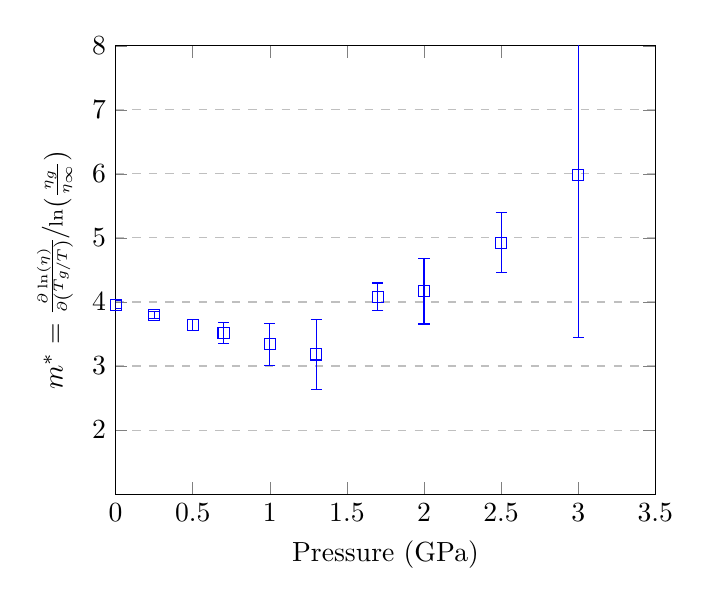
\begin{tikzpicture} 
				\begin{axis}[
					ylabel={$m^*=\nicefrac{\frac{\partial \ln(\eta) }{\partial \left(\nicefrac{T_g}{T}\right)}}{\ln\left( \frac{\eta_g}{ \eta_\infty}\right )}$},
					xlabel={Pressure ($\si{\giga\pascal}$)},
					xmin=0, xmax=3.5,
					ymin=1, ymax=8,
					xtick={0,.5,1,1.5,2,2.5,3,3.5},
					ytick={2,3,4,5,6,7,8},
					ymajorgrids=true,
					grid style=dashed
					]
					\addplot+[only marks, mark=square,error bars/.cd, y dir=both,y explicit]
					coordinates { 
						(0.7,3.512883)    +- (0,.168) 
						(1.3,3.181076)    +- (0,.546)
						(0,3.958805)    +- (0,.064)  
						(2,4.16682)    +- (0,.51) 
						(2.5,4.922827)    +- (0,.468)
						(.25,3.801)    +- (0,.0535) 
						(1,3.339)    +- (0,.328) 
						(1.7,4.083887)    +- (0,.213) 
						(0.5,3.638201)    +- (0,.088)
						(3,5.98637)    +- (0,2.547)  
					};
				\end{axis} 
			\end{tikzpicture}
		\end{minipage}
		\hspace{0.05\textwidth}
		\begin{minipage}[t]{.475\textwidth}		
			\begin{tikzpicture} 
				\pgfplotsset{set layers}
				%
				\begin{axis}[
					xmin=0,xmax=3.5,
					ymin=-10,ymax=20,
					ytick={-5,0,5,10,15,20},
					axis y line*=left,
					ymajorgrids=true,
					grid style=dashed,
					xlabel={Pressure ($\si{\giga\pascal}$)},
					ylabel style = {align=center},
					ylabel={$\Delta T_g$ ($\si{\kelvin}$)}
					]
					\addplot +[mark=square] table [only marks,x=a, y=b, col sep=comma] {RegressionError.csv};
				\end{axis}
				%
				\begin{axis}[
					xmin=0,xmax=3.5,
					ymin=-2,ymax=10,
					axis y line*=right,
					axis x line=none,
					ylabel style = {align=center},
					ylabel={$\Delta m^*$},
					]
					\addplot +[mark=triangle] table [only marks,x=c, y=d, col sep=comma] {RegressionError.csv};
				\end{axis}
			\end{tikzpicture}
		\end{minipage}\hfill
	}
	\caption{Left:  Scaled fragility as a function of pressure derived from classic VTF fits to the data of Cook \etal with the glass transition point included as determined \via our \tgp isochron.  Right: The error in terms of under or over-estimation of the glass transition temperature, $\Delta T_g$, due to extreme extrapolation of the VTF model as demonstrated in \fig \nolinebreak \ref{figure:CookMiss}, is provided ($\color{blue}\square$) along with error in scaled fragility ($\color{blue}\triangle$) calculated from these extrapolated models. } \label{figure:CookFragIGP}
\end{figure}

The right side of \fig \nolinebreak \ref{figure:CookFragIGP} shows the under or over estimation of the glass transition temperature as a function of pressure derived from the classic VTF fits to the data of Cook \etal without the \tgp isochronal data. The initial under-estimation of the glass transition temperature for the two lowest pressures is followed by a trend of increasing over-estimation up to about $1.7\;\si{\giga\pascal}$ where we continue to over-estimate the transition temperature, albeit to an increasingly lesser degree.  However the error in fragility associated with this over-estimation in glass transition temperature continues to increase in a fairly linear fashion leading to the excessively high fragilities at increased pressure observed by Cook \etal in \fig \nolinebreak \ref{figure:CookFrag}.

It is worth noting here that, though viscosity data of Cook \etal was predominately taken along isotherms as this was experimentally favorable, they did manage to obtain two pseudo-isobaric runs at $0.7$ and $1.3\;\si{\giga\pascal}$ on which they then used interpolation between free-volume fits to their isothermal data to correct for slight deviations of pressure.  Though this process was extremely time intensive, it did provide them with two isobaric runs over a large temperature range addressing the issue of insufficient data points.  It should be noted, however, that these data are still limited to well below the glass transition.  Due to the larger number of data points associated with these pseudo-isobaric runs, the error associated with the fragility estimations are significantly smaller and these two points are included ($\color{red}\triangle$) in the left side of \fig \nolinebreak \ref{figure:CookFrag}.  These two higher-confidence points would alone imply a potentially constant fragility below $1.5\;\si{\giga\pascal}$\textemdash albeit at a significantly higher scaled fragility $(m^*\approx 5.7)$.  

Beyond $1.5\;\si{\giga\pascal}$ the fragility steadily increases by $\Delta m^*\approx 7.8$ and then remain approximately constant within uncertainty beyond $2.5$ to $3\;\si{\giga\pascal}$ before rapidly diverging due to extrapolation errors again.  This general trend of increasing fragility is, in the loosest sense, in "agreement" with subsequent published works as will be demonstrated.  This leads to the conclusion that the viscosity data of Cook \etal is perhaps significantly more reliable than may have been assumed and much of its error, as perhaps expected, is predominately the result of these extrapolation issues. Our method of employing \tgp data to diminish this extrapolation error significantly decreases the error associated with these fragility estimations however it is still limited\textemdash particularly at elevated pressures.  More data is needed in the region of interest to further define the slope at the glass transition\textemdash data which has since been provided by other groups and is included in \fig \ref{figure:CookProninReiser}.    

Other methods such as photon correlation spectroscopy and dielectric loss spectroscopy certainly exist and there is no shortage of data for glycerol dynamics within the literature around the vicinity of the glass transition, though generally limited to cryogenic measurements at low pressures.  If the issues with these fragility calculations do in fact stem predominately from the lack of data in critical regions rather than the efficacy of the data itself, then supplementation of their data with other literature data in critical regions should allow accurate determinations of fragility as a function of pressure. Glycerol data taken by several different groups extend over different pressure and temperature regions and include both viscosity and $\alpha$-relaxation measurements, making glycerol a prime candidate for a surface fragility analysis, similar to what will also be done for cumene in \chap\nolinebreak \ref{chap:PCS}.  

To add further validation to Cook \etal's data at lower pressures, the same analysis method of implementing the \tgp data point to constrain the VTF fits in the vicinity of the glass transition was applied to the rolling ball data obtained by McDuffie and Kelly and the associated fragilities calculated \nolinebreak\cite{McDuffie}.  Though these fragility values were much more in line with other works implementing dynamic light scattering (Brodin \nolinebreak\cite{Brodin}), and dielectric spectroscopy (Reiser \etal \nolinebreak\cite{Reiser}, Pronin \nolinebreak\cite{Pronin}, and McDuffie and Kelly \nolinebreak \nolinebreak\cite{McDuffie}), they all follow the same general trend of constant fragility below $1\;\si{\giga\pascal}$.  The increasing trend mentioned by Pronin and Reiser \etal is simply not statistically significant.  This seems to suggest a strong increase in fragility does not occur until beyond $1\;\si{\giga\pascal}$.  This may be due to the general expected trend of decreasing fragility with increasing pressure is being approximately balanced by the early onset of hydrogen bond breaking giving rise to a relatively constant fragility in this range.

\section{Structural Relaxation Surface}

	Experimentally, it is often difficult to obtain truly isobaric data at high-pressure. When a fluid is confined within a pressure vessel or diamond--anvil cell, changes in temperature inevitably induce changes in pressure due to thermal expansion.  In their PCS measurements, Cook \etal went to considerable lengths to interpolate between data points in order to construct pseudo--isobaric data runs.  Of considerable utility, therefore, would be a framework capable of fitting relaxation data acquired over broad ranges of temperature and pressure (or specific volume) without requiring strict isobaric or, for that matter isothermal, constraints.  This motivates the development of a continuous structural--relaxation surface.

	To this end, the Andersson--Andersson constrained surface model provided in \app \ref{app:AndersonSurface} is employed, extending the classic isobaric Vogel--Tammann--Fulcher (VTF) formalism to account for pressure dependence through polynomial expansions of pressure--dependent parameters. A more rigorous mathematical development of this model is presented in \sect \ref{sec:surface}.  Here, only the essential structure of the surface and the physical constraints imposed upon it are discussed.
	
	For most liquids, a substantial body of high--quality ambient--pressure data exists in the literature, obtained using a variety of experimental probes of structural relaxation and viscosity, owing to the relative experimental accessibility of this thermodynamic region\textemdash glycerol being no exception. \fig \ref{figure:1barglycerol} presents an Angell plot of almost all atmospheric--pressure data collected for this work, together with a fit to the classic isobaric VTF model. This atmospheric-pressure isobar serves as a primary constraint for the relaxation surface.
	
	It should be noted that the Cook \etal data have been excluded from this atmospheric--pressure constraint. The \tgp point, shown on the same Angell plot at a location corresponding to $\tau = 220~\si{\second}$ as determined from thermodynamic scaling of the low--pressure \tgp data in \fig \ref{figure:GlycerolIGPLinear}, was likewise not included in the fit, though it exhibits excellent agreement with the data what was included. 
	
	At the time the atmospheric-pressure data were fit, the degree to which the intercept method of thermodynamic scaling accurately determines the isochronal value associated with the Andersson--Andersson regression of the \tgp data was not yet established.  One peripheral insight arising from the development of these surface models is the realization that, for liquids whose dynamics conform to thermodynamic scaling, this approach provides a robust means of identifying the precise isochrone represented by a given \tgp data run. Even in cases where thermodynamic scaling may not strictly apply, the atmospheric--pressure constraint provides an independent verification of this isochronal value, as the Andersson--Andersson regression through the \tgp data must intersect the atmospheric VTF isobar.
	
	The Andersson--Andersson regression through the \tgp data provides an additional constraint to be imposed on the surface construction. Specifically, the VTF expression is solved for the zero--mobility temperature $T_0$ in terms of the pressure--dependent glass--transition temperature $T_g(P)$ and subsequently reinserted into the VTF form, yielding  \eqn \ref{eqn:glycerolSurfaceModel}.  Here, $T_g(P)$ is taken from the Andersson--Andersson fit to the \tgp data provided in \app \ref{app:GlycerolIGP}.  
	This procedure results in a relaxation surface constrained both at atmospheric pressure and along an isochrone corresponding to $\tau \approx 220~\si{\second}$.
	
	The remaining four parameters comprising the coefficient vectors $\vec{d}$ and $\vec{t}$ are treated as free parameters and are determined using a Levenberg--Marquardt optimization algorithm to conform the surface to the remaining data\textemdash excluding the \tgp and 1-bar data. \fig \ref{figure:CookSurfaceFit} displays this constrained surface together with the Cook \etal data, shown for initial parameter estimates. The atmospheric isobaric constraint and the isochronal \tgp constraint are indicated by solid black curves on the surface.
	
	It is emphasized that the surface is not fit to the Cook \etal data. Because they measured viscosity directly via rolling--ball viscometry, whereas all other data in this chapter probe the structural $\alpha$--relaxation time, the decision was made to include the Cook \etal data only for qualitative comparison.  The Cook \etal viscosity data were scaled using an appropriate high--frequency shear modulus $G_\infty$ to permit comparison with the relaxation--time surface.
	
	Glycerol viscosity and relaxation data from several sources are shown, along with the Cook \etal rolling ball data obtained from within a DAC, in \fig \nolinebreak \ref{figure:GlycerolSurfaceFitWithError} \nolinebreak\cite{Brodin,McDuffie,Paluch,Pronin,Reiser}.  It is clear that data is actually in excellent agreement with other literature data further bolstering the case that the vast majority of the error within the Cook \etal fragility measurements lies in the extreme extrapolation to the glass transition.  The inclusion of the \tgp isochronal data, though addressing the issue of extrapolation to a significant extent, ultimately provides insufficient accommodation for an accurate determination of the rate of vitrification with increasing pressure in the vicinity of the glass transition, $T_g$.  More data is needed to define the slope near $T_g$ to obtain an isobaric fragility in consensus with other contributors to the literature, \ie Pronin, Paluch, \etc  
	
	In short, there never was any issue with the validity of Cook \etal's viscosity data before extrapolation.  As we will see, it is in reasonable agreement with other measurements of vitrification or associated alpha relaxation behavior.  It is only the lack of data to provide constraint to the VTF fit in key locations, specifically in the vicinity of $T_g$, that gives rise to the incongruence of the Cook \etal fragility estimations with literature values, \ie the slope in the vicinity of $T_g$ is poorly constrained.  The addition of the \tgp isochronal data is not itself sufficient to provide the necessary constraint on this slope for reliable estimations of fragility.  However, as we will here demonstrate, only one additional experimentally trivial, constraint is needed for Cook \etal's data to provide fragility values as a function of pressure in excellent agreement with the current literature consensus\textemdash an ambient isobar.  
	
		\pgfplotsset{table/search path={Chapters/glycerol/SupportingFiles},}
		\begin{figure}[!htbp]
		\resizebox{0.95\textwidth}{!}{%
		\begin{tikzpicture}
		\begin{axis}[restrict z to domain=0:18,zmax=18,zmin=0,
		width=0.9\textwidth,
		xmax=400, xmin=180,
		ymax=3, ymin=0,
		xtick={200,240,280,320,360,400},
		ytick={1,2,3},
		ztick={5,10,15},
		xlabel = Temperature $(\si{\kelvin})$,
		ylabel = Pressure  $(\si{\giga\pascal})$,
		zlabel = {$\log_{10} <\tau> (\si{\pico\second})$},
		title = {Andersson--Andersson Constrained Surface Model With Cook \etal Viscosity Data},
		]
		
		\addplot3[forget plot, only marks, scatter = false, mark options={draw=blue, fill=blue}] table [x=temp, y=pressure, z=logtau, col sep=comma] {fitsurfaceGlycerolDataCook.csv};
		
		\addplot3[no marks,very thick, scatter] table [x=temp, y=pressure, z=logtau, col sep=comma] {1BarRegression.csv};
		
		\addplot3[no marks,very thick, scatter] table [x=temp, y=pressure, z=logtau, col sep=comma] {TgpRegressionshort.csv};
		
		\addplot3[
		mesh,
		samples=23,
		samples y=31,
		domain=180:400,y domain=0:3,
		draw=black       
		]
		{(-6.0104+.176307*(y*10)+(188.376*(1+.0365618*(y*10))^(.488759)*(19.0464-.848505*(y*10)+.0222398*(y*10)^2-.000214289*(y*10)^3))/(-188.376*(1+.0365618*(y*10))^(.488759)+x+(19.0462-.848505*(y*10)+.0222398*(y*10)^2-.000214289*(y*10)^3)*x/(39.7601-.176307*(y*10))))/ln(10)
		};
		
		\end{axis}
		\end{tikzpicture}
		}
		\caption{Cook \etal's rolling ball viscosity data is here provided along with the Andersson-Andersson constrained surface model, given initial approximations for the fit parameters, described in \app\nolinebreak \ref{app:AndersonSurface}. The surface is extended to $3\;\si{\giga\pascal}$ corresponding to the highest pressures for which Cook \etal obtained data \protect\nolinebreak\cite{Cook2}. The mesh lines correspond to constant-temperature and constant-pressure slices (isotherms and isobars), spaced at 10~K and 0.1~GPa, respectively.}
		\label{figure:CookSurfaceFit}
		
	\end{figure}

\fig \nolinebreak\ref{figure:CookSurfaceFit} shows all of Cook \etal's raw viscosity data provided by reference \nolinebreak\cite{Cook2} fit to the Andersson-Andersson constrained surface model described in \app\nolinebreak \ref{app:AndersonSurface}.  The Solid black isobaric line at atmospheric pressure, through which the surface is constrained, is well described in \fig \nolinebreak \ref{figure:1barglycerol}, along with the supporting data.  This 1-bar regression was also used to define the isochrone for the \tgp curve\textemdash the second solid black line extending across the top of the surface in \fig \nolinebreak \ref{figure:CookSurfaceFit}.  The glycerol \tgp data fit to a standard Andersson-Andersson model is provided in \app\nolinebreak \ref{app:GlycerolIGP} and corresponds to an isochronal pressure-temperature relationship at $\tau\approx10^{14}\;\si{\pico\second}$ through which the surface is also constrained.  

This Andersson-Andersson constrained surface model, fit to the Cook \etal viscosity data, allows for a determination of fragility as a function of pressure in similar fashion to that obtained for cumene in \fig \nolinebreak \ref{figure:fragilityPressure}.  The resulting functional dependence of isobaric fragility is plotted as a solid black line in \fig \nolinebreak \ref{figure:CookProninReiser} above and found to be in significantly greater agreement with Pronin, Reiser \etal, and other more recent works up to $2.5\;\si{\giga\pascal}$.  This result, along with the excellent constrained surface fit, suggest that Cook \etal's data could not be lacking significantly in quality.  

	\begin{figure}[!htbp]
	\resizebox{0.95\textwidth}{!}{%
	\begin{tikzpicture}
	\begin{axis}[
	colorbar,
	point meta min=-10, 
	point meta max=20,
	restrict z to domain=0:18,zmax=18,zmin=0,
	width=0.9\textwidth,
	xmax=400, xmin=180,
	ymax=5, ymin=0,
	ytick={1,2,3,4,5},
	ztick={5,10,15},
	xlabel = $Temperature (\si{\kelvin})$,
	ylabel = $Pressure (\si{\giga\pascal})$,
	zlabel = {$Log_{10} <\eta> (cP)$},
	title = {Glycerol Relaxation Data},
	legend style={only marks, at={(0,1)},anchor=north east}
	]
	
	\addplot3[only marks, scatter, scatter src=explicit] table [x=temp, y=pressure, z=logtau, meta=error, col sep=comma] {fitsurfaceGlycerolDataCook.csv};
	\addlegendentry{{\scriptsize Cook \etal \cite{Cook2}}}
	
	\addplot3[only marks, mark=square*, scatter, scatter src=explicit] table [x=temp, y=pressure, z=logcp, meta=error, col sep=comma] {fitsurfaceGlycerolDataPaluch.csv};
	\addlegendentry{{\scriptsize Johari and Whalley \cite{JohariWhalley}}}
	
	\addplot3[only marks, mark=triangle*, scatter,scatter src=explicit] table [x=temp, y=pressure, z=logcp, meta=error, col sep=comma] {fitsurfaceGlycerolDataPronin.csv};
	\addlegendentry{{\scriptsize Pronin \cite{Pronin}}}
	
	\addplot3[only marks, mark=star, scatter, scatter src=explicit] table [x=temp, y=pressure, z=logcp, meta=error, col sep=comma] {fitsurfaceGlycerolDataReiser.csv};
	\addlegendentry{{\scriptsize Reiser \etal \cite{Reiser}}}
	
	\addplot3[only marks, mark=x, scatter, scatter src=explicit] table [x=temp, y=pressure, z=logtau, meta=error, col sep=comma] {fitsurfaceGlycerolData1bar.csv};
	\addlegendentry{{\scriptsize 1-Bar \cite{Brodin,Pronin,Ngai}}}
	
	\addplot3[only marks, mark=diamond*, scatter, scatter src=explicit] table [x=temp, y=pressure, z=logtau, meta=error, col sep=comma] {fitsurfaceGlycerolDataTgp.csv};
	\addlegendentry{{\scriptsize \tgp}}
	
	\addplot3[no marks,very thick, scatter, scatter src=explicit] table [x=temp, y=pressure, z=logtau, meta=error, col sep=comma] {1BarRegression.csv};
	
	\addplot3[no marks,very thick, scatter, scatter src=explicit] table [x=temp, y=pressure, z=logtau, meta=error, col sep=comma] {TgpRegression.csv};
	
	%\addplot3[only marks, scatter] table [x=temp, y=pressure, z=logtau, col sep=comma] {fitsurfaceGlycerolDataMcDuffie.csv};
	
	\addplot3[
	point meta=0,
	mesh,
	samples=23,
	samples y=51,
	domain=180:400,
	y domain=0:5
	]
	{
		14.3733
		- ((8.27174 + 2.44421*y - 0.153233*y^2)
		* (126.678 + 13.237*y - 0.540195*y^2 - 0.0459642*y^3))
		/(-126.678
		+ 188.376*(1 + 0.365618*y)^(0.488759)
		- 13.237*y
		+ 0.540195*y^2
		+ 0.0459642*y^3)
		+ ((8.27174 + 2.44421*y - 0.153233*y^2)
		* (126.678 + 13.237*y - 0.540195*y^2 - 0.0459642*y^3))
		/(-126.678
		- 13.237*y
		+ 0.540195*y^2
		+ 0.0459642*y^3
		+ x)
	};
	
	
	\end{axis}
	
	\node[] at (15,-.5) {$\% Error$}; 
	\end{tikzpicture}
	}
	\caption{The surface shown corresponds to the model described in \app\nolinebreak\ref{app:AndersonSurface}, fit to a compilation of glycerol relaxation data from Johari and Whalley, Pronin, and Reiser \etal. The Cook \etal, \tgp, and atmospheric data were not included in the fit, but are represented on the surface. Data points are colored by their percent deviation from the fitted surface, highlighting systematic trends in the residuals. The mesh lines correspond to constant-temperature and constant-pressure slices (isotherms and isobars), spaced at 10~K and 0.1~GPa, respectively.}
	\label{figure:GlycerolSurfaceFitWithError}
	
\end{figure} 

In \fig \ref{figure:GlycerolSurfaceFitWithError} we have the model described in \app\nolinebreak \ref{app:AndersonSurface} fit to a large selection of glycerol relaxation data from multiple contributers, including Pronin \etal \cite{Pronin}, Johari and Whalley \cite{JohariWhalley}, and Reiser \etal \cite{Reiser}.  The same \tgp and 1-bar constraint was imposed here as was implemented in \fig\nolinebreak \ref{figure:CookSurfaceFit}.  The color scale represents percent deviation of the data from the surface.  Note how the high-pressure Pronin data begins to diverge from the surface, approaching an error as high as $20\%$.  This data was still included in the fit as it conforms well to the surface at higher temperatures and lower viscosities\textemdash only tending away from the surface in a region where the \tgp constraint does not allow the data significant influence over the fit parameters.

\fig \nolinebreak\ref{figure:GlycerolSurfaceFitWithError} shows the same Andersson-Andersson constrained surface model fit to a larger selection of literature data including Cook \etal's rolling ball viscosity data.  The same \tgp and atmospheric constraints are applied.  Here the Actual \tgp data is provided on the surface yet not included in the fit.  It is found that Cook \etal's rolling ball viscosity data is in excellent agreement with other works including Johari and Whalley, Pronin, Paluch, and Reiser \etal thus we must conclude that the Cook \etal data is very reliable\textemdash the issue of increasingly overestimated fragility arising predominately from extreme extrapolation \nolinebreak\cite{Johari,Paluch,Pronin,Reiser}.  It should be noted that the four isobaric data sets extracted from Pronin's \fig 3 in reference \nolinebreak \cite{Pronin} do trend increasingly above the fit surface at higher pressures yet agree with Cook \etal and others at lower pressures.  The toroidal pressure cell used by Pronin and described in reference \cite{Khvostantsev} may not have provided a hydrostatic sample to the degree that was assumed\textemdash a scenario which would certainly explain the data's increasing divergence from the \tgp isochrone at higher pressures and lower temperatures as the glass transition is approached.  The Pronin isobars are still in reasonable agreement with Cook \etal's data at higher temperatures where hydrostatic conditions are assured, even at the highest pressure.  However this data was included as it does not heavily effect the surface at lower pressures where it is in reasonable agreement with the rest of the data yet allows us to extend this fit surface up to $5\;\si{\giga\pascal}$.  Thus it should be assumed that our calculated fragility above $3\;\si{\giga\pascal}$ may have reasonable error associated with it and any fine structure is not of high confidence.  It should be noted that this Pronin data could be replaced with DPCS measurements at high pressure near the glass transition just as was done with cumene. Molecular simulations may provide high-pressure fast dynamics at extreme temperatures.  

\begin{figure}[!htbp]
	\centering
	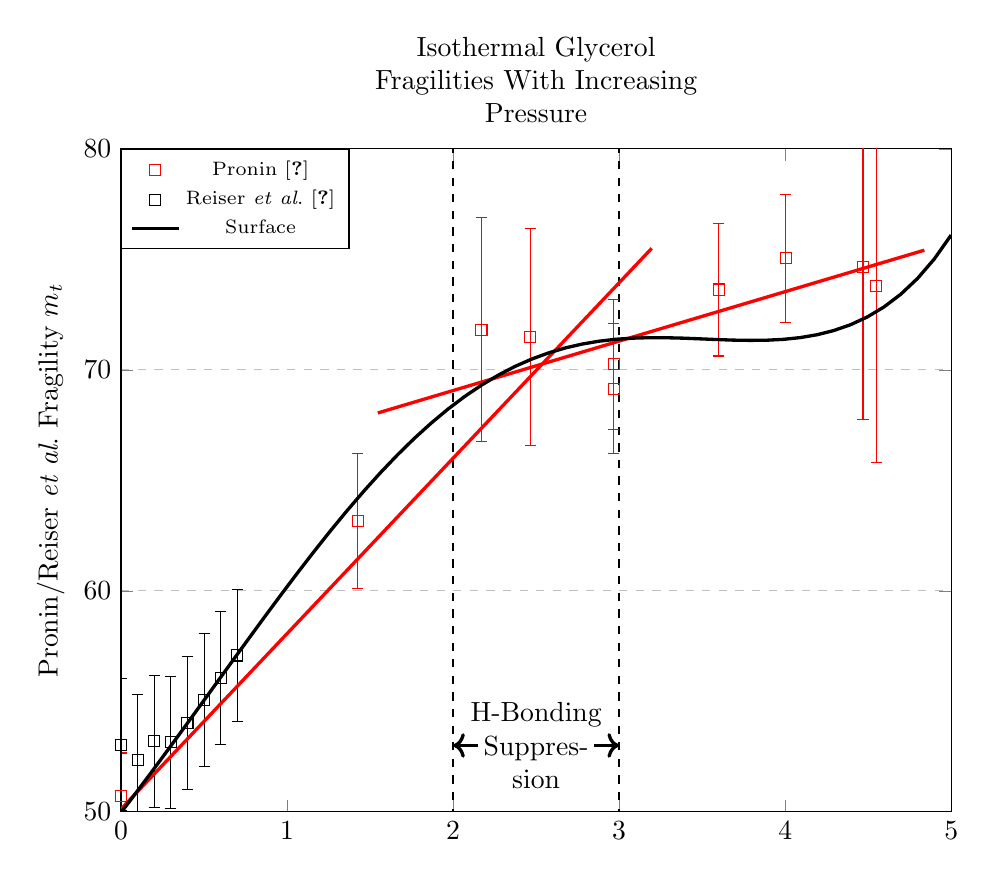
\begin{tikzpicture} 
	
	\begin{axis}[
	title={\parbox{0.35\textwidth}{\centering Isothermal Glycerol Fragilities With Increasing Pressure}},
	samples=100,
	width=\linewidth,
	height=10cm,
	xmin=0, xmax=5,
	ymin=50, ymax=80,
	xtick={0,1,2,3,4,5},
	ytick={50,60,70,80},
	ylabel style = {align=center},
	ylabel={Pronin/Reiser \etal Fragility $m_t$},
	ymajorgrids=true,
	grid style=dashed,
	legend style={at={(0,1)},anchor=north west}
	]
	
	\draw[black,dashed, thick] (2,40)--(2,80);
	\draw[black,dashed, thick] (3,40)--(3,80);
	\draw[black,very thick, ->] (2.85,53)--(3,53);
	\draw[black,very thick, ->] (2.15,53)--(2,53);
	\node[] at (2.5,53) {\parbox{0.15\textwidth}{\centering H-Bonding Suppression}};
	
	\addplot+[red,only marks, mark=square,error bars/.cd, y dir=both,y explicit]
	coordinates { 
		(0,50.72324)    +- (0,1.938) 
		(1.426686,63.16297)    +- (0,3.0665)
		(2.170432,71.81292)    +- (0,5.063)  
		(2.464173,71.4947)    +- (0,4.918) 
		(2.966801,70.25072)    +- (0,2.95)
		(2.966979,69.1514)    +- (0,2.95)
		(3.599749,73.63549)    +- (0,3.0087) 
		(4.002432,75.05304)    +- (0,2.89296) 
		(4.468517,74.64802)    +- (0,6.914) 
		(4.54875,73.80906)    +- (0,7.985)      
	};
	\addlegendentry{{\scriptsize Pronin \cite{Pronin}}}
	
	\addplot+[black,only marks, mark=square,error bars/.cd, y dir=both,y explicit]
	coordinates { 
		(0,53.03688)    +- (0,3) 
		(.1,52.32513)    +- (0,3)
		(.2,53.18672)    +- (0,3)  
		(.3,53.13989)    +- (0,3) 
		(.4,54.01085)    +- (0,3)
		(.5,55.05975)    +- (0,3)
		(.6,56.05246)    +- (0,3) 
		(.7,57.07326)    +- (0,3)        
	};
	\addlegendentry{{\scriptsize Reiser \etal \cite{Reiser}}}
	
	\draw[red, very thick] (0,50.1228) -- (3.195876,75.49795);
	\draw[red, very thick] (1.546392,68.049) -- (4.838,75.4161);
	
	\addplot+[no marks,very thick, black] {0.434294*(38.2465-0.1569*(x*10))*(1+(38.2465-0.1569*(x*10))/(19.0462-.75566*(x*10)+.0188737*(x*10)^2-.000176531*(x*10)^3))};
	\addlegendentry{{\scriptsize Surface}}
	
	\end{axis} 
	\end{tikzpicture}
	
	\caption{Fragility estimations from Pronin ($\color{red}\square$) and Reiser \etal's ($\color{black}\square$) data are shown above.  The pressure dependence of fragility derived from isobaric temperature derivatives of the Andersson-Andersson surface model described in \app\nolinebreak \ref{app:AndersonSurface}, fit to the data of Cook \etal, Johari and Whalley, Pronin, Paluch, and Reiser \etal, is shown as a solid black line.  The upward curve in fragility approaching $5\;\si{\unit{\giga\pascal}}$ is likely a relic due to the previously discussed issues with the Pronin data at high pressure as well as the surface being generally unconstrained by data beyond this pressure. }
	\label{figure:FinalFragilities}
\end{figure}

The calculated fragility as a function of pressure arising from the Andersson-Andersson surface model from \fig \nolinebreak \ref{figure:GlycerolSurfaceFitWithError} including data from Cook \etal, Johari and Whalley, Pronin, Paluch and Reiser \etal is provided in \fig \ref{figure:FinalFragilities}\textemdash extending our fragility measurements out to $5\;\si{\giga\pascal}$.  The red lines show Pronin's original estimation of the fragility behavior with increasing pressure as was lifted directly from his \fig~4 in reference \nolinebreak \cite{Pronin}. This result shows unequivocally Cook \etal's rolling ball viscosity data to be in excellent agreement with other literature measurements of viscosity, $\eta$, and $\tau_\alpha$.  The Andersson--Andersson constrained surface model relieves us of the experimental burden of maintaining isobaric conditions during data acquisition, which is very difficult to accomplish in a diamond anvil cell. It also avoids reliance on free-volume models, where a reliable equation of state may not be available, as well as isothermal models such as the modified VTF equation of \eqn \ref{eqn:ModifiedVTFPressureClassic}, which will appear in our discussion of cumene but may not adequately capture the transition from a hydrogen-bonded liquid to one exhibiting more van der Waals behavior, such as glycerol.

\section{Equation of State and Thermodynamic Scaling} \label{sec:GlycerolScaling}

Simple van der Waals glass-forming liquids have been shown to obey density scaling, in which the relaxation dynamics conform to a single function of the form $\tau \propto (T V^\gamma)^{-1}$, where $\gamma$ is a material-dependent constant. In \sect\nolinebreak \ref{sec:tdscaling}, this behavior is demonstrated explicitly for cumene, where density scaling is found to hold over a compression approaching 29\%. In the case of a simple liquid such as cumene, the intermolecular interactions are well approximated by the Lennard--Jones potential,
\begin{equation}
	U(r)=4\epsilon\left[\left(\frac{\sigma}{r}\right)^{12}-\left(\frac{\sigma}{r}\right)^6\right],
	\label{eqn:LennardJones}
\end{equation}
for which the short-range repulsive term scales as $r^{-12}$. Because structural relaxation is governed primarily by these steep repulsive interactions at close intermolecular separation, the dynamics are expected to reflect an effective inverse power-law form dominated by this repulsive contribution.

This factor $\gamma$ has been shown to depend on the intermolecular potential energy landscape, which may be approximated as $U(r)\sim\left(\frac{\sigma}{r}\right)^{3\gamma}$, where $r$ is the spatial separation between any two molecules and $\sigma$ is a material constant \nolinebreak\cite{Roland2005RPP, Roland3,Coslovich}. Within this framework, one expects an effective scaling of the form $U(r)\sim r^{-3\gamma}$, with $3\gamma = 12$ in the limiting case of a purely inverse power-law repulsive interaction of the form $r^{-12}$. Real liquids, however, are not strictly inverse power-law systems due to the presence of attractive interactions and molecular complexity, and thus are expected to exhibit effective exponents that deviate from this ideal value. In the case of cumene $\gamma\approxeq4.77$\textemdash indicating a slightly steeper effective repulsive interaction than that of an ideal Lennard--Jones fluid. The dynamics of such liquids are therefore strongly driven by simple free-volume considerations, and thus we expect thermodynamic scaling to hold with increasing pressure, as is observed in the case of cumene.

However, in the case of strongly associated liquids such as glycerol, intermolecular interactions include directional hydrogen bonding, which introduces additional structure into the potential energy landscape beyond simple isotropic repulsion. While all intermolecular interactions depend on temperature and pressure, the presence of such directional bonding can inhibit the emergence of a single effective inverse power-law description, and thus thermodynamic scaling is not generally expected to hold in these systems. Nevertheless, several such liquids do exhibit thermodynamic scaling\textemdash at least over limited ranges of pressure and temperature, where the influence of specific interactions is reduced and the dynamics become increasingly governed by short-range repulsive forces.

Glycerol is one such example, having a measured scaling parameter within the literature in the range of $1.4\leq \gamma \leq 1.6$ \nolinebreak\cite{Reiser,Kyaw}.  This lower value for $\gamma$ is expected given that free-volume will play a reduced role in the dynamics of associated liquids as molecular mobility is no longer just a matter of thermal diffusion past nearest neighbors exhibiting van der Waals repulsion, but also will require energy to break hydrogen bonds with said neighbors.  However these values for $\gamma$ were all determined at relatively low pressures\textemdash on the order of $0.1\;\si{\mega\pascal}$, \ie, near ambient pressure.  Yet we see in \fig \ref{figure:FinalFragilities} a shift in the fragility behavior as a function of pressure occurring between $2$ and $3\;\si{\giga\pascal}$ which has been attributed to a suppression of hydrogen bonding. If hydrogen bonding between glycerol molecules is sufficiently suppressed at very high pressures, one might expect glycerol to behave much more like a simple van der Waals liquid with a scaling parameter, $\gamma$, much closer to 4 as the potential energy landscape no longer is heavily influenced by these suppressed intra-molecular interactions.  

\pgfplotsset{table/search path={Chapters/Glycerol/SupportingFiles},}
\begin{figure}[!htbp]
	\centering
	\begin{tikzpicture} 
	\begin{axis}[
	title={Thermodynamic Scaling of \tgp Isochrone},
	ylabel={Log$(T)$},
	xlabel={-Log$(V)$},
	ymin=2.25, ymax=2.55,
	xmin=-.08, xmax=.08,
	scaled x ticks=true,
	xtick scale label code/.code={},
	xlabel={$-\log(V)\;(\times 10^{-2})$},
	%xtick={0,.002,.004,.006,.008,.01},
	%ytick={0,2,4,6,8,10,12,14,16},
	width=0.9\textwidth
	]
	
	\addplot table [only marks, x=LogV, y=LogT, col sep=comma] {glycerolTGPscaling.csv};
	
	\addplot expression[domain=-.08:.04,mark=none,red]{
	1.5359*x+2.3667};

	\addplot expression[domain=0.01:0.08,mark=none,red]{
	3.6536*x+2.3155};

	\draw[black,dashed, thick] (0.01842,2.25) -- (0.01842,2.55);
	\draw[black,dashed, thick] (0.03535,2.25) -- (0.03535,2.55);
	
	\draw[black,very thick, ->] (0.01842,2.28)--(0.03535,2.28);
	\draw[black,very thick, ->] (0.03535,2.28)--(0.01842,2.28);
	\node[font = {\fontsize{8 pt}{12 pt}\selectfont}] at (0.02688,2.295) {\parbox{0.15\textwidth}{\centering H-Bonding Suppression}};
	
	\node[rotate=60] at (0.06,2.50) {\parbox{0.15\textwidth}{\centering y=3.65x+2.32}};
	
	\node[rotate=36] at (-.03,2.3) {\parbox{0.15\textwidth}{\centering y=1.54x+2.37}};
	
	\node[] at (-0.06,2.5) {\parbox{0.15\textwidth}{\centering Increasing Pressure}};
	\draw[black,line width=3pt, ->] (-0.045,2.5)--(-0.03,2.5);

	\end{axis}
		
	\end{tikzpicture}
	\caption{The linearized isochronal glycerol \tgp data shows a transition from an H-bonded liquid at low pressure with a corresponding scaling factor of $\gamma\approxeq1.54$ to a liquid which behaves more like one experiencing a simple van der Waals potential at higher pressures, where H-boding is suppressed, exhibiting a scaling factor of $\gamma\approxeq3.65$.  The region between the dotted vertical lines corresponds the region indicated in \fig \ref{figure:FinalFragilities} previously.  The intersection of the two linear regimes is self consistent with the results of Pronin at approximately $2.5\;\si{\giga\pascal}$.  It is also worthy of note that the average y-intercept of 2.35 implies a \tgp isochrone of $\tau\approx 220\;\si{\unit{\second}}$.}
	\label{figure:GlycerolIGPLinear}
\end{figure}

In \fig \ref{figure:GlycerolIGPLinear}, the glycerol \tgp data provided in \app \ref{app:GlycerolIGP} is linearized and plotted to determine the scaling parameter.  Rather than assuming thermodynamic scaling a priori, we instead test for its validity by considering the expected form
\begin{equation}
	\tau \propto (T V^\gamma)^{-1},
	\label{eqn:GlycerolScaling}
\end{equation}
which, upon rearrangement, implies
\begin{equation}
	\log(T) = -\gamma \log(V) + \mathrm{const}.
	\label{eqn:GlycerolScalingLinear}
\end{equation}
Thus, if thermodynamic scaling holds, a plot of $\log(T)$ versus $-\log(V)$ should yield a linear relationship, with the slope directly corresponding to the scaling parameter $\gamma$.

The region between the dotted lines once again corresponds to that in \fig \ref{figure:FinalFragilities}\textemdash where pressure suppression of hydrogen bonding becomes prominent.  The results are quite compelling.  Two distinct regions emerge.  At low pressure we find a scaling factor $\gamma=1.54$ consistent with literature values. At high pressures, well within the region where hydrogen bonding is assumed to be sufficiently suppressed, we find a significantly greater slope corresponding to $\gamma=3.65$ consistent with what might be expected of a simpler van der Waals liquid. A clear transition occurs between $2$ and $3\;\si{\giga\pascal}$\textemdash consistent with our fragility results from our Andersson-Andersson contained surface model as well as Pronin's analysis.

\pgfplotsset{table/search path={Chapters/Glycerol/SupportingFiles},}
\begin{figure}[!htbp]
	\centering
	\resizebox{0.95\textwidth}{!}{%
	\begin{tikzpicture} 
	\begin{axis}[
	colorbar,
	colorbar style={xshift=1cm,
		yticklabel pos=left,
		yticklabel style={anchor=east},
		rotate=0},
	title={Thermodynamic Scaling of Surface Data},
	ylabel={Log$(\eta)$},
	xlabel={$\frac{10^{-4}}{TV^\gamma}$},
	ymin=1, ymax=16,
	xmin=0.9, xmax=3,
	%xtick={0,.002,.004,.006,.008,.01},
	%ytick={0,2,4,6,8,10,12,14,16},
	width=0.9\textwidth,
	legend style={only marks, at={(0,1)},anchor=north west}
	]
	
	\addplot [scatter,point meta=explicit,point meta min={0}, point meta max={6.55}] table [only marks, x=xcook, y=ycook, meta=Pcook, col sep=comma] {glycerolTGPScaledData2.csv};
	\addlegendentry{{\scriptsize Cook \etal \cite{Cook2}}}
	
	\addplot [mark=square,scatter,point meta=explicit,point meta min={0}, point meta max={6.55}] table [only marks, x=xJandW, y=yJandW, meta=PJandW, col sep=comma] {glycerolTGPScaledData2.csv};
	\addlegendentry{{\scriptsize Johari and Whalley \cite{Johari}}}
	
	\addplot [mark=triangle,scatter,point meta=explicit,point meta min={0}, point meta max={6.55}] table [only marks, x=xpronin, y=ypronin, meta=Ppronin, col sep=comma] {glycerolTGPScaledData2.csv};
	\addlegendentry{{\scriptsize Pronin \cite{Pronin}}}
	
	\addplot [mark=star, scatter,point meta=explicit,point meta min={0}, point meta max={6.55}] table [only marks, x=xreiser, y=yreiser, meta=Preiser, col sep=comma] {glycerolTGPScaledData2.csv};
	\addlegendentry{{\scriptsize Reiser \etal \cite{Reiser}}}
			
	\addplot [mark=diamond,scatter,point meta=explicit,point meta min={0}, point meta max={6.55}] table [only marks, x=xtgp, y=ytgp, meta=Ptgp, col sep=comma] {glycerolTGPScaledData2.csv};
	\addlegendentry{{\scriptsize \tgp}}
	
	\node[rotate = 55] at (2.5,8) {\parbox{0.15\textwidth}{\centering High Pressure}};
	\node[rotate = 55] at (1.6,8) {\parbox{0.15\textwidth}{\centering Low Pressure}};
	
	\end{axis}
	
	\node[] at (15.2,-.5) {$\si{\giga\pascal}$};
	
	\end{tikzpicture}
	}

	\caption{The results of thermodynamic scaling of glycerol for all low pressure data ($<2\;\si{\giga\pascal}$) with a scaling factor of $\gamma = 1.54$ and high-pressure data ($>3\;\si{\giga\pascal}$) with a scaling factor of $\gamma = 3.65$.}
	\label{figure:GlycerolIGPScaling}
	
\end{figure}

All of the glycerol data that falls outside of the transition region between $2$ and $3\;\si{\giga\pascal}$ provided by Cook \etal, Johari and Whalley, Pronin, Reiser \etal, and our \tgp data exhibit a reasonable degree of thermodynamic scaling along one of two curves.  The results of this scaling are provided in \fig \nolinebreak \ref{figure:GlycerolIGPScaling}.  We see that all of the Cook \etal data scales nicely even well into the intermediate pressure regimen-perhaps due to the relative high temperatures allowing for molecular mobility which facilitates hydrogen bonding at these higher pressures. The Johari and Whalley data, on the other hand, is all at relatively low to intermediate temperatures and a clear pressure dependent divergence from good thermodynamic scaling is observed as pressure increases and hydrogen bonding begins to be suppressed.  All of this still relies on an extreme extrapolation of the Tait equation of state for which Bridgman only provides data up to approximately $1.2\;\si{\giga\pascal}$ however thermodynamic scaling is possible, albeit in two distinct regimens each with different scaling factor, $\gamma$.  Where hydrogen bonding is not being suppressed we find a scaling factor $\gamma=1.54$ that reflects a liquid for which free-volume plays a diminished role in the dynamics. 

Once again we note that the high-pressure data of Pronin \etal taken in the toroidal pressure cell seems to scale at lower pressures or higher temperatures however, as vitrification sets in at higher pressure the data peels away from the trend expected if thermodynamic scaling were to hold in precisely the same manner that it peeled away from the Andersson-Andersson constrained surface fit previously. It appears once again as if the reported pressures are lower than what the dynamics would imply.  As this discrepancy is occurring only at the highest pressure and in the region where vitrification is rapidly increasing, it stands to reason that they have underestimated the prominence of pressure gradients within their toroidal cell. The lower pressure data, even in the vicinity of the glass transition, scales nicely just as it conformed very well to the relaxation surface.  However as pressures increase the odds of significant pressure gradients inside the cell increases greatly.  
\graphicspath{{Chapters/PCS/Figures/}}

\chapter{Photon Correlation Spectroscopy in a Diamond Anvil Cell} \label{chap:PCS}
\section{Justification}\label{sec:PCSIntro}

\sect \ref{sec:probes} describes several probes commonly implemented to measure molecular dynamics in glass-forming systems as the timescale associated with structural relaxation changes by as much as fifteen orders of magnitude while the liquid vitrifies into a glass. Wolynes and Lubchenko assert in their discussion of Dielectric Spectroscopy (DS) that this technique is uniquely suited to track molecular dynamics in glass-forming systems over this large dynamic range. Indeed, when taken as a whole, the multitude of methods that fall under the banner of DS provide an astonishing range of measurement for relaxation times from $\tau \approx 1 \,\si{\nano\second}$ up to $\tau > 1000 \,\si{\second}$\nolinebreak\cite{Wolynes}. However, many of these methods do not lend themselves well to the geometric constraints and experimental limitations of a diamond anvil cell (DAC) or other high-pressure apparati. For example, reflection or transmission techniques require that the sample be arranged in a macroscopic coaxial configuration. The methods that may lend themselves well—most notably frequency response and time-domain analysis—are only now being developed in the context of the DAC\cite{Peng,Chan,Ransom2017DACDielectric}.

As shown in \fig \ref{figure:Probes}, depolarized photon correlation spectroscopy (DPCS) covers a dynamic range similar to that of conventional dielectric spectroscopy (DS) frequency-response analysis, extending in principle from approximately $10 \,\si{\nano\second}$ to beyond one thousand seconds, and provides a direct probe of the structural $\alpha$-relaxation. When combined with depolarized Brillouin light scattering (DBLS), the accessible dynamic range of light scattering techniques is extended by several additional decades toward shorter times, approaching a total span of nearly 15 orders of magnitude. A relatively narrow gap remains between the fastest dynamics accessible to DPCS and the slowest dynamics probed by DBLS. In principle, this intermediate regime is accessible via dielectric spectroscopy in the radio-frequency (RF) range; however, such high-frequency dielectric measurements have proven difficult to implement under the constraints of high-pressure diamond anvil cell environments and have seen limited application in this context.  

Although both DPCS and DS offer comparable windows for measuring molecular dynamics, they differ fundamentally in how those dynamics are accessed. DPCS is a passive technique that probes spontaneous fluctuations arising from the stochastic thermal evolution of the system, whereas dielectric spectroscopy is inherently a driven measurement, relying on an externally applied electric field to induce dipolar reorientation. While linear-response conditions are typically assumed, the driven nature of DS raises the possibility that the modes most strongly excited by the applied field may not uniquely correspond to the collective structural relaxation of the material.

Additionally, DPCS does not require electrode structures within the sample volume; only optical access is needed, making it a particularly accessible option for extending measurements of structural relaxation into the diamond anvil cell. Despite these differences, both methods are worthy of development, as they possess complementary strengths and limitations.

Dielectric spectroscopy provides a direct probe of structural relaxation only when the dielectric susceptibility faithfully reflects the orientational dynamics of the liquid under study. In such cases, the primary dielectric loss peak may be identified with the bulk $\alpha$-relaxation. However, this correspondence is not guaranteed. DS is intrinsically sensitive to dipolar reorientation, and when molecular dipoles are associated with specific subunits or segments, the measured response may be dominated by local or segmental dynamics rather than collective structural rearrangement. 

This limitation is well illustrated in polymeric systems, where dipole moments may be associated with specific molecular subunits rather than the global structure. In such cases, dielectric spectroscopy can be dominated by local or segmental dynamics that are decoupled from collective structural relaxation. For example, in poly(dimethylsiloxane) (PDMS), the dipole moment is oriented transverse to the polymer backbone, such that the dielectric response reflects only segmental motion rather than global chain dynamics\cite{Wrzesinska2020}. While polymeric systems provide a particularly clear manifestation of this effect, the underlying issue is more general: whenever dipolar reorientation does not uniquely track collective structural rearrangement, the dielectric $\alpha$-process may not faithfully represent bulk relaxation. This motivates the use of complementary probes that couple more directly to density or orientational fluctuations of the material as a whole.

Depolarized photon-correlation spectroscopy couples to fluctuations in the anisotropic component of the molecular polarizability tensor. As a result, DPCS is inherently sensitive to orientational and structural dynamics associated with collective molecular rearrangement, while remaining insensitive to purely isotropic density fluctuations. This selectivity provides a complementary view of structural relaxation dynamics, though it too comes with inherent limitations, perhaps the most significant being that the molecular system must exhibit a sufficiently strong polarizability anisotropy to generate a measurable depolarized scattering signal.

Molecules with extremely high symmetry, such as carbon tetrachloride or sulfur hexafluoride, lack significant anisotropic (off-diagonal) components of the dielectric susceptibility tensor and therefore do not generate an observable depolarized scattering signal. While such highly symmetric systems rarely form molecular glasses due to their strong tendency toward crystallization, they provide a useful conceptual limit that illustrates the symmetry-imposed constraints of DPCS. 

Experimentally relevant glass formers typically exhibit some degree of molecular anisotropy.  The same geometric features that give rise to orientational frustration and enable glassy dynamics in the first place also tend to generate off-axis components of the dielectric susceptibility tensor. Consequently, glass-forming systems generally lend themselves to producing at least some measurable depolarized scattering signal.

Despite the respective limitations of both depolarized photon--correlation spectroscopy (DPCS) and dielectric spectroscopy (DS), many systems may lend themselves equally well to either probe, at least in principle. A clear illustration of this complementarity is provided by \textit{n}-propanol, which possesses a substantial dipole moment of 1.57~Debye~\cite[p.~9-48]{CRC1997} and is therefore well suited to dielectric measurements, while also exhibiting sufficient molecular anisotropy to produce a measurable depolarized scattering signal, as is commonly observed in comparable small-molecule glass-forming liquids~\cite[p.~114]{Berne}\cite{Brodin}. Although its polarizability anisotropy is smaller than that of aromatic liquids such as cumene, \textit{n}-propanol represents an intermediate case in which both dielectric spectroscopy and DPCS can probe relaxation dynamics in the liquid.

Notably, \textit{n}-propanol is a small, comparatively rigid molecule, and therefore does not exhibit the segmental or sub--chain dynamics that can complicate the interpretation of dielectric spectra in polymeric or highly flexible systems. Nevertheless, this does not guarantee that dielectric spectroscopy directly probes the structural $\alpha$--relaxation. In monohydroxy alcohols such as \textit{n}-propanol, the dielectric response is characterized by a nearly Debye-like relaxation, while mechanical and structural probes reveal markedly different relaxation behavior, indicating pronounced decoupling in both timescale and spectral shape. This decoupling has been attributed to the presence of hydrogen-bonded microheterogeneities within the liquid structure \cite{Angell2000}.

While this dielectric relaxation arises from intermolecular dipolar correlations, it does not directly correspond to the structural $\alpha$--relaxation. Consequently, DS in \textit{n}-propanol reflects collective dipolar fluctuations associated with hydrogen--bonded correlations, rather than providing a direct measure of bulk structural dynamics, and its amplitude and spectral shape may be influenced by the evolving network structure \cite{Davidson,Angell2000}.

\begin{figure}[!htbp]
	\centering
	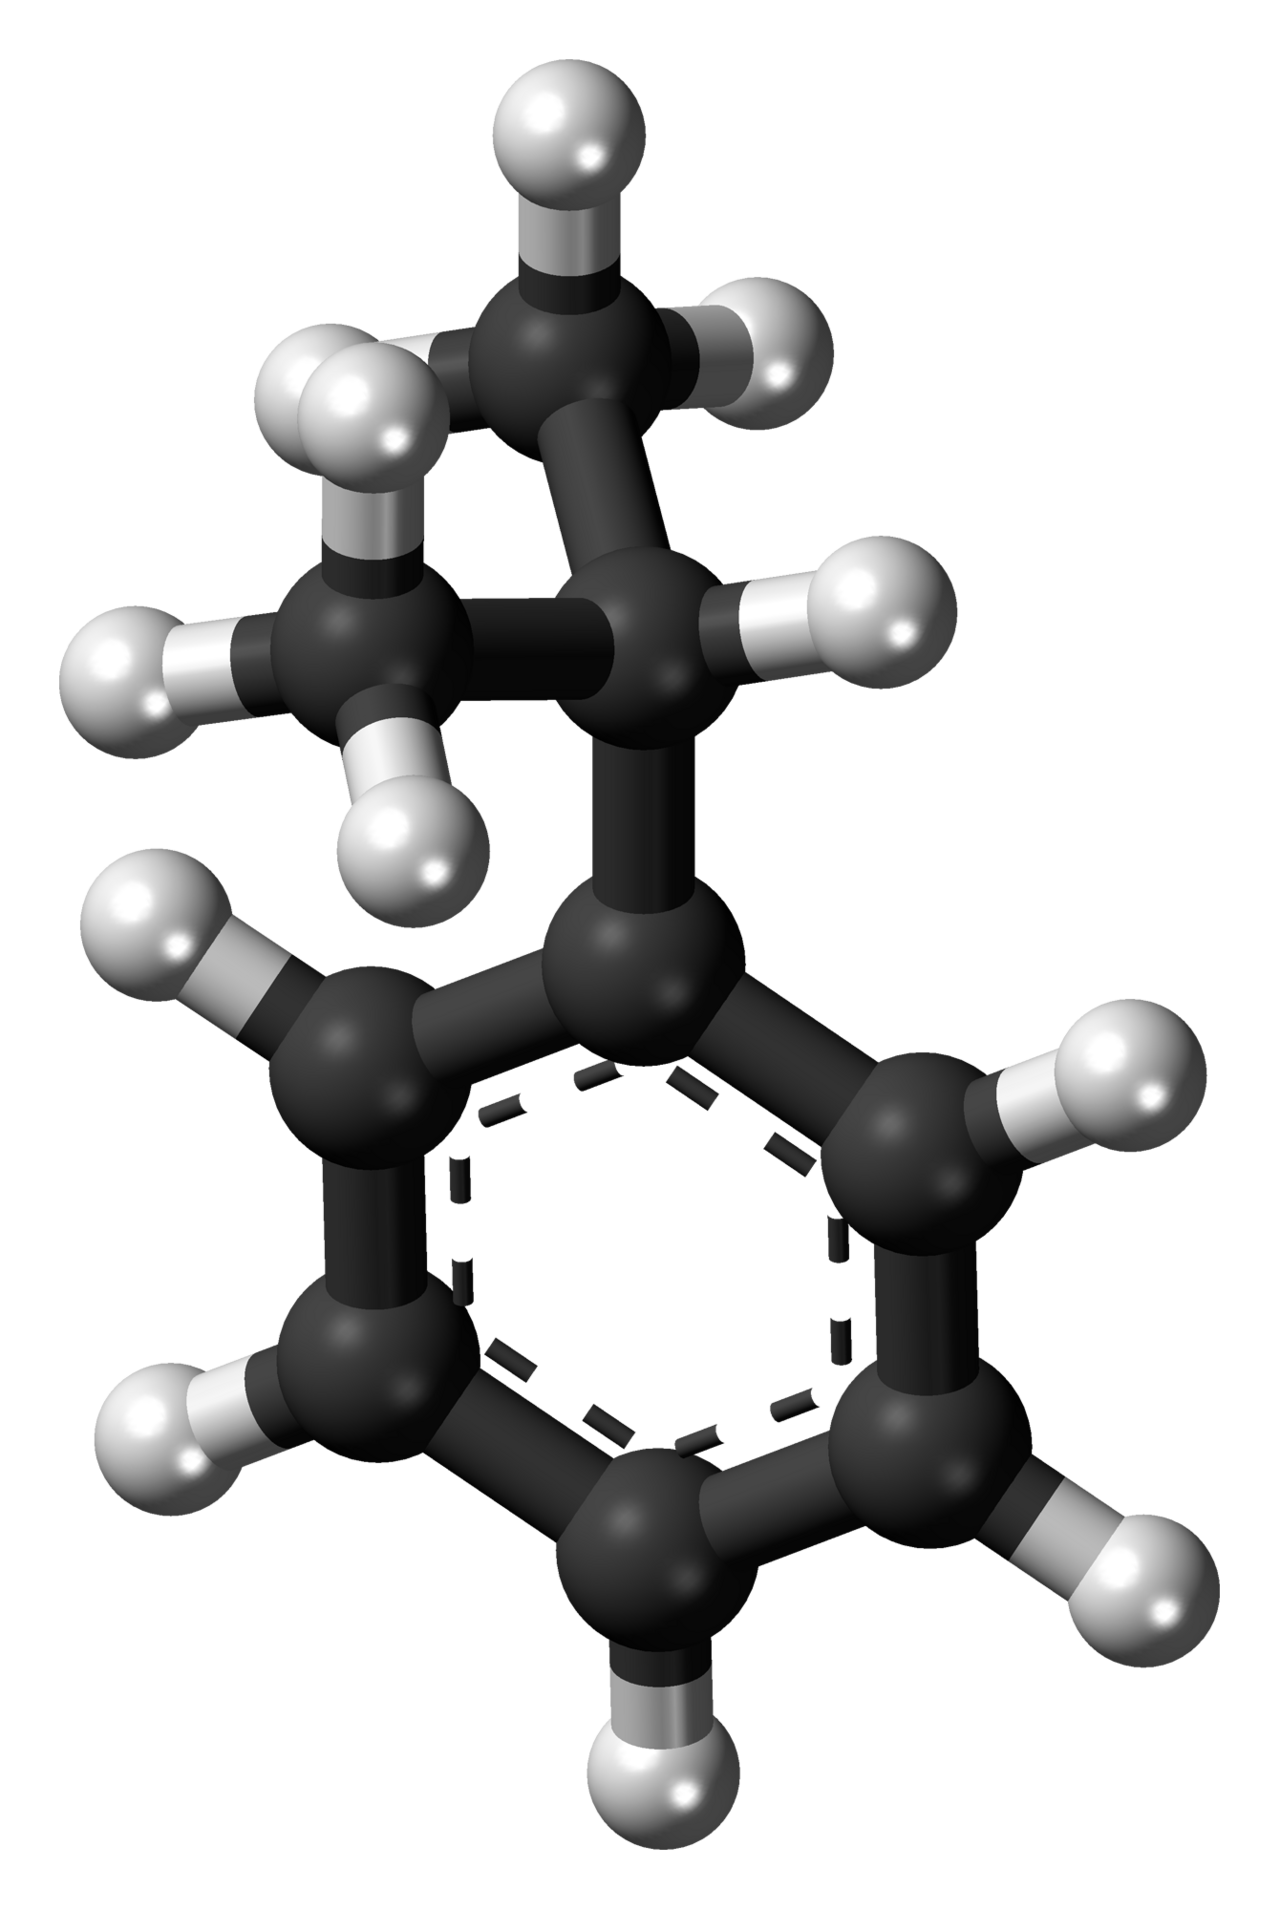
\includegraphics[width=0.35\textwidth]{Chapters/PCS/Figures/Cumene_3D_ball.png}
	\caption{Molecular structure of cumene (isopropylbenzene). The rigid aromatic ring contributes to a large polarizability anisotropy, while the absence of hydrogen bonding results in comparatively simple van der Waals–dominated relaxation dynamics.}
	\label{figure:CumeneStructure}
\end{figure}

Cumene (isopropylbenzene), shown in \fig\ref{figure:CumeneStructure}, represents a complementary case that is particularly favorable for both probes. Its rigid aromatic structure gives rise to a large polarizability anisotropy, making it exceptionally well suited to DPCS measurements, while the absence of hydrogen bonding or internal molecular flexibility ensures that its dielectric response, though weaker due to the modest permanent dipole moment, remains closely tied to the collective structural $\alpha$--relaxation. Consequently, although \textit{n}-propanol yields a weaker depolarized scattering signal and cumene a weaker dielectric response, both systems lend themselves naturally to investigation by either technique, with each probe accessing the same underlying structural relaxation dynamics. Even in such systems, DPCS may be a preferable probe simply because it requires only optical access to the sample.

In conclusion, in systems with strong molecular anisotropy but complex or heterogeneous dipolar dynamics, such as polymeric liquids or molecular systems with independently mobile dipolar subunits, dielectric spectroscopy may preferentially probe local or segmental relaxations rather than collective structural rearrangement. In these cases, DPCS remains directly sensitive to the bulk $\alpha$-relaxation, providing a direct probe of structural relaxation dynamics by accessing the stochastic thermal evolution of the system without coupling to driven, local modes \cite{Roland,Patterson}.

\begin{table}[!htbp]
	\centering
	
	\tabletitle{Representative molecular systems illustrating DS and DPCS sensitivity}
	\vspace{0.5em}
	
	\begin{tabular}{lccccc}
		\hline
		Molecule & Glass Former & $\chi_{i\neq j}$ & DS Sensitivity & Anisotropic Signal \\
		\hline
		Cumene (isopropylbenzene) & Yes & Large & Direct $\alpha$ & Very strong \\
		\textit{n}-Propanol & Yes & Moderate & Decoupled & Moderate \\
		Poly(vinyl acetate) & Yes & Large & Segmental & Strong \\
		Glycerol & Yes & Moderate & Mixed & Moderate \\
		\hline
		Carbon tetrachloride (CCl$_4$) & No & Vanishing & Weak & Weak \\
		Sulfur hexafluoride (SF$_6$) & No & Vanishing & Weak & Weak \\
		\hline
	\end{tabular}
	
	\label{tab:DSvsDPCS}
	
	\tabledescription{Off-diagonal $\chi_{i\neq j}$ denotes the relative magnitude of anisotropic contributions to the dielectric susceptibility tensor responsible for depolarized scattering. Highly symmetric molecules are included as conceptual reference cases, though their poor glass-forming ability limits their relevance here. In such systems, DPCS yields little to no measurable depolarized signal due to the near-isotropy of the susceptibility tensor, and DS shows no meaningful correlation with collective structural relaxation. For \textit{n}-propanol, ``Decoupled'' indicates that the dominant dielectric relaxation does not correspond directly to the structural $\alpha$--process, but instead reflects dipolar dynamics associated with hydrogen--bonded correlations.}
\end{table}

Having established the complementary strengths and limitations of dielectric spectroscopy and depolarized photon-correlation spectroscopy, it is important to emphasize the experimental challenges associated with extending DPCS into the diamond anvil cell. The most significant of these is the exceedingly small sample volume, typically on the order of $\sim 10\,\si{\nano\liter}$. In conventional cuvette-based light-scattering experiments, the scattered signal is collected from an extended region illuminated by a focused beam that may span several hundred microns, resulting in effective scattering volumes on the order of a few nanoliters. In the DAC geometry, by contrast, the illuminated region is typically confined to only a few tens of microns.

Under these conditions, it is necessary to ensure that a sufficient number of statistically independent scatterers contribute within the effective scattering volume so that the detected field obeys the Gaussian statistics assumed by photon correlation spectroscopy. This consideration is particularly relevant in experiments where scattering arises from a low number density of discrete mesoscopic scatterers, such as microspheres undergoing Brownian motion in a host liquid, for which the effective number of scatterers within the probe volume may be limited. For homogeneous liquids, however, light scattering originates from ubiquitous thermal density fluctuations, and even picoliter-scale scattering volumes contain an effectively macroscopic number of dynamically independent fluctuators. As a result, the Gaussian-field assumption remains well satisfied for pure liquids, provided that parasitic scattering from the gasket or diamond anvils is adequately suppressed.

This brings us to another concern regarding DPCS in a DAC\textemdash stray spectral reflections from every optical interface, together with unavoidable scattering from the gasket material, are collected alongside the desired signal. As a result, isolating the true scattering volume and suppressing background contributions is a dominant experimental challenge.

Herbst \etal addressed many of these difficulties in their effort to extend photon correlation spectroscopy (PCS), identical in application to DPCS but without polarization analysis, into the DAC as a probe of viscosity at high pressures \nolinebreak\cite{Herbst}. By analyzing the Brownian motion of polystyrene spheres suspended in the liquid, they obtained reasonable agreement with known values of methanol viscosity at pressures up to 2.9~GPa. Although successful, this approach has not reappeared in the literature since its publication, likely because the experimental complexity is disproportionate to its limited applicability: the method probes viscosities only up to approximately 90~cP.

In principle, the accessible viscosity range could be extended by employing smaller tracer particles and performing longer-timescale autocorrelations. Nevertheless, this approach remains orders of magnitude removed from the glass-transition regime, where viscosities reach $10^{15}$~cP. Indeed, in the same year, Cook, working with Herbst \etal, demonstrated centrifuge rolling-ball viscometry in a DAC at viscosities exceeding $10^{9}$~cP \nolinebreak\cite{Cook}. However, rolling-ball techniques are inherently limited to viscosities for which a macroscopic object can traverse the liquid within a practical experimental timescale and therefore cannot be extended to the glass transition.

By contrast, DPCS in a DAC could, at least in principle, access the glass transition and beyond if correlation spectra could be obtained directly from intrinsic density fluctuations of the pure liquid, rather than from nanoparticles suspended within it. The fundamental obstacle to this approach is the extremely weak scattering intensity associated with such fluctuations. In the Rayleigh regime, the intensity of light scattered from spherical particles scales with the sixth power of the particle radius \nolinebreak\cite{Sinclair}. Consequently, the scattering intensity arising from intrinsic density fluctuations, whose characteristic correlation lengths remain nanometric even in the presence of cooperative dynamics, will be many orders of magnitude weaker than that obtained from the 90~nm polystyrene spheres used by Herbst \etal. All of the challenges associated with small sample volumes are therefore dramatically amplified when attempting to extend PCS or DPCS measurements to pure liquids in the DAC.

One goal of this chapter is to describe the process of extending depolarized photon-correlation spectroscopy (DPCS) into the diamond anvil cell, thereby establishing a new probe of slow dynamics at very high pressures, up to and beyond the glass transition. Given the severe experimental constraints outlined above, it is essential to begin with a molecular system that maximizes the depolarized scattering signal. Aromatic liquids such as isopropylbenzene (cumene), with their large anisotropic polarizability arising from the benzene ring, produce exceptionally strong depolarized scattering signals and therefore represent near-optimal candidates for such a proof-of-concept study.

Cumene, a simple van der Waals–bonded glass-forming liquid, was selected both for this reason and for the availability of independent fast-dynamics data from Brillouin light-scattering measurements \cite{Li1995CumenePRL}. Together, these data allow characterization of relaxation dynamics over an exceptionally broad range of timescales, spanning from tens of picoseconds to hundreds of seconds. In addition, a separate study provided direct measurements of the pressure dependence of the glass-transition temperature via the \tgp method \cite{RansomPRL} described in \chap \ref{sec:IGPintro}. Agreement among these independent probes provides strong evidence for the efficacy of DPCS as a reliable probe of slow dynamics at high pressures in a DAC.

As previously mentioned, the light scattered from intrinsic density fluctuations within a pure liquid was expected to be exceedingly weak compared to undesired sources such as specular reflections from the diamond surfaces and gasket interfaces. An initial attempt therefore assumed heterodyne operation, deliberately collecting both the desired scattered signal and accompanying elastic and surface-scattered light, with the latter serving as a local oscillator. The combined light was directed onto the photomultiplier tube (PMT), with neutral-density filters used to attenuate the total intensity to a safe count rate. A polarizer was employed primarily to isolate the depolarized component of the scattering signal required for DPCS; however, the finite extinction ratio of the cube polarizer used in this setup allowed a significant fraction of elastically scattered and specularly reflected light to pass through. In practice, the collected light comprised contributions from these sources, rendering a homodyne/heterodyne determination difficult. Under these conditions, it is perhaps not surprising that no correlation decay could be resolved even after several hours of data acquisition.

It was therefore clear that spatial filtering was required to reject as much of the residual local oscillator as possible. This, however, introduced a new problem\textemdash physically locating the scattering volume within an exceedingly large region of optical splash. A telescopic viewfinder could be lowered into place to image the interior of the DAC for alignment purposes, but this proved insufficient. The experimenter was still left to blindly raster the collected light across the pinhole in an attempt to isolate a correlation decay signal. Given the uncertainty regarding how long signal averaging would be required before a clear decay emerged, and the tedious nature of blindly rastering over a relatively large area, this approach was impractical.

The present effort to implement DPCS within a DAC can be viewed as an extension of the strategy first demonstrated by Demoulin \etal, who showed that time-domain correlation of scattered intensity provides direct access to structural relaxation on timescales spanning microseconds to seconds\nolinebreak\cite{Demoulin}. Their analysis of undercooled glycerol established the utility of the Cole--Davidson distribution in describing broad, nonexponential relaxation spectra. Later, Lindsey and Patterson demonstrated the correspondence between the Cole--Davidson and Williams--Watts functions, providing a practical means of translating between frequency- and time-domain analyses\nolinebreak\cite{Lindsey}. Taken together, these works justify the approach pursued here: by developing the experimental capability to isolate weak depolarized scattering from liquids under extreme confinement in a DAC, one gains a direct probe of structural relaxation that is theoretically continuous with both ultrasonic/frequency-domain results and with the broad body of photon correlation data analyzed in the time domain. Furthermore, high-pressure DPCS data provides direct access to structural relaxation dynamics in glass-forming systems that are closely related to those probed by DBLS in the frequency domain, which accesses much shorter time scales down to about a ps \cite{47,119}, with a narrow intermediate regime separating the two techniques.
\graphicspath{{Chapters/PCS/Figures/}}

\section{Experimental Details}\label{sec:PCSExp}

The complete experimental layout is shown in \fig \ref{figure:PCSsetup} and is described below along with the process of obtaining an autocorrelation signal.
\begin{figure}[!htbp]
	\centering
	\begin{tikzpicture}
		\node (img) {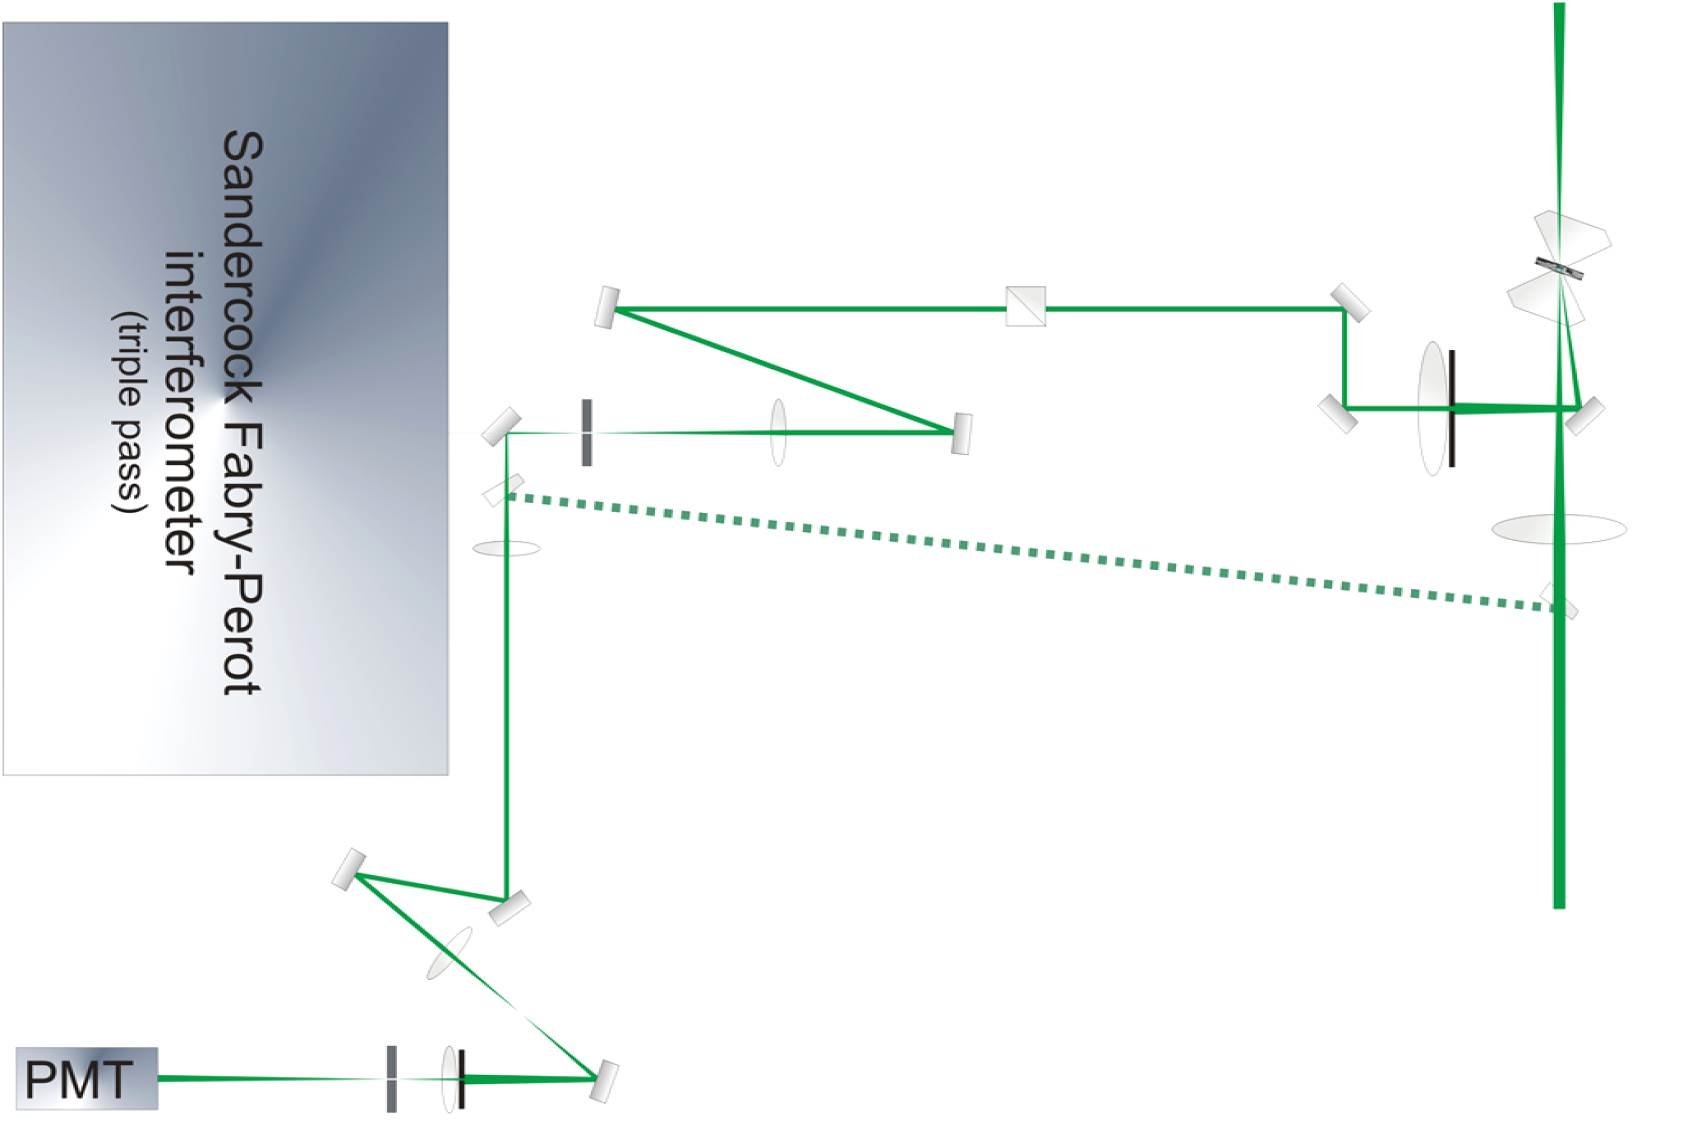
\includegraphics[width=\textwidth]{PCSsetup.jpg}};
		\node at (7.6,2.8) {a};
		\node at (7.6,1.2) {b};
		\node at (1.8,3.0) {c};
		\node at (-3.5,1.75) {d};
		\node at (-3.0,-4.2) {e};
	\end{tikzpicture}
	\caption{Major components of the experimental setup for DPCS: (a) DAC, (b) 1~cm mirror to redirect the scattered signal, (c) polarizer, (d) flip mirror to redirect the signal from the interferometer to the autocorrelator. The spectrum analyzer is a Sandercock-type tandem Fabry--P\'erot interferometer operated in a multi-pass (triple-pass tandem) configuration, corresponding to a total of six passes through the etalons, thereby providing substantially enhanced contrast and spectral resolution compared to a single- or double-pass design. Irises and pinholes are shown as black and gray bars, respectively. The dashed line represents a failed attempt to provide a local oscillator for heterodyne DPCS analysis.}
	\label{figure:PCSsetup}
\end{figure}
A Coherent Innova 306 actively locked single-mode Ar\textsuperscript{+} medium-frame laser operating at 514~nm provided the light source. To ensure the highest level of power stability, the laser was allowed to warm up at a set current near its operating point for one to two hours. At that stage, manual adjustments were made to the rear mirror to maximize output. Power and mode tracking were then enabled at 1~W output, and the laser was left to warm up for an additional half hour, with occasional alignment adjustments to minimize the operating current. Approximately once per week, the mode-tune algorithm was executed following this warm-up procedure.  

A set of reflective neutral-density filters allowed this 1~W output to be incrementally adjusted between 1 and approximately 30~mW while maintaining the power stability of the laser. Because the expected scattering signals are exceedingly weak, laser stability was of paramount importance. Future improvements to this system may include the implementation of cross-correlation, which would reduce dependence on power stability and enable analysis of even weaker scattering systems.

As shown in \fig \ref{figure:PCSsetup}, the beam is focused through the DAC located at position (a). The DAC is mounted on a four-axis stage that allows for $x$, $y$, $z$, and $\theta$ translations of the cell. What we will refer to as the $z$-axis is aligned along the incoming focused laser beam and is the primary axis that must be adjusted during signal optimization, as will be discussed shortly. The $\theta$ axis lies in the plane of the optical table and allows the DAC to be rotated as shown. In a typical Brillouin experiment, the DAC is rotated away from the collection mirror in order to reduce the amount of spectrally reflected light mixed with the desired signal.  

It should be noted that changes to $\theta$ do not affect the scattering vector $\vec{q}$, which is geometrically fixed by the collection mirror at location (b). This $1 \,\si{\centi\meter}$ diameter mirror is placed as close as possible to the incoming beam without occultation in order to closely approximate a 180\textdegree{} backscattering geometry. The external angle between the incoming beam and the path from the scattering volume to the center of the mirror is less than 3\textdegree. However, due to the indices of refraction of both the diamonds and the liquid sample, the actual scattering angle is significantly smaller—estimated to be less than 1\textdegree.  

The collimating optic that follows is preceded by an iris, which is used in Brillouin studies to restrict the scattering vector $\vec{q}$ collected. Here, however, the iris is opened reasonably wide but still serves to limit the collection cone, effectively providing a degree of low-resolution spatial filtering by rejecting off-axis light. The collimated light then passes through a polarizer at location (c), which may be removed for alignment purposes and replaced to select the depolarized component of the scattering signal. The beam height is then adjusted by the next two mirrors, placed intentionally after the polarizer, to match the input height of the interferometer. A $200 \,\si{\micro\meter}$ pinhole provides spatial filtering, and the flip mirror at location (d) is rotated out of the path of the incoming light to allow for spectral analysis.

\pgfplotsset{table/search path={Chapters/PCS/Figures}}
\begin{figure}[!htbp]
	\centering
	\begin{tikzpicture}
		\begin{axis}[
			ylabel={PMT counts},
			xlabel={Frequency (\si{\giga\hertz})},
			xmin=-15, xmax=15
			]
			\addplot table [only marks, x=a, y=b, col sep=comma] {BrillouinLA.csv};
		\end{axis}
	\end{tikzpicture}
	\caption{Typical Brillouin spectrum with the polarizer removed. The rapidly forming longitudinal acoustic (LA) peaks are used to optimize the DAC position for maximum signal. The polarizer is then reinserted and rotated until the LA peaks are suppressed, ideally leaving only the depolarized signal for DPCS analysis.}
	\label{figure:LAmodes}
\end{figure}

Even at relatively low pressures, far from the glass transition, light scattered from longitudinal acoustic modes gives rise to classic Brillouin peaks, as shown in \fig \ref{figure:LAmodes}. Here the spatial filtering may be optimized via maximizing the intensity of these longitudinal acoustic mode peaks. This is done predominately by adjusting the before-mentioned $z$-axis which translates the DAC along the path of the incoming laser light such that the collection area being focused onto the pinhole at location (d) corresponds to the liquid sample between the diamond culets. The fact that this Brillouin spectra forms significantly more quickly than the much weaker depolarized spectrum allows for rapid optimization of the spatial filtering. Once this is achieved, the polarizer is replaced and oriented to suppress the LA-modes—passing only the depolarized component of the scattered light. The mirror at location (d) is then flipped up, redirecting the spatially filtered light towards the autocorrelator PMT. The next focusing optic re-collimates the light after the pinhole and is followed by two mirrors to once again adjust the height of the beam to match the input height of the autocorrelator optics. The autocorrelator setup itself was previously designed for use with a 1cm cuvette and it was desirable not to strip the system of this capability. As such, the original PCS system was left intact so that a cuvette and oven could be placed at location (e) or removed at will. To accommodate for DPCS in the DAC, the lens following the height adjustment mirrors creates an image of the DAC sample at location (e) which the PCS setup then further spatially filters before directing the light to the PMT.  

\subsection{Homodyne \vs Heterodyne} \label{sec:HomoHeto}

As mentioned in \sect \ref{sec:PCSIntro}, DPCS may be performed in either a homodyne (self-beating) or a heterodyne (local oscillator) arrangement. What was not previously discussed is the requirement that one must be squarely within one of these two regimes in order to avoid prohibitively complex analysis. Elimination of the heterodyne component in the collected light signal is a significant hurdle when attempting PCS within a DAC. The surrounding structure, the edges of the gasket, every surface interface, and even inevitable dust on the diamond table scatter light with appreciable intensity. This problem is further exacerbated by the exceedingly small scattering volume (on the order of a nanoliter), making it easy for the heterodyne contribution to be comparable to—or even significantly stronger than—the light scattered from the sample volume.  

In depolarized studies, much of the heterodyne signal is immediately rejected by the polarizing prism. However, due to the finite extinction ratio of the polarizer a substantial component of the local oscillator inevitably bleeds through. Herbst \etal devoted considerable effort to addressing this challenge when first achieving PCS in a DAC\nolinebreak\cite{Herbst}. They were able to approach near-homodyne conditions through proper orientation of the DAC to deflect spectral reflections away from the collection optics, combined with spatial filtering of the collected light.

Their method, however, becomes increasingly difficult to apply when one wishes to directly probe density fluctuations in a pure liquid. Despite similar sample volumes, Herbst \etal measured the thermal diffusion of $\sim 90~\si{\nano\meter}$ polystyrene spheres and thus benefited from orders-of-magnitude greater scattering intensity. Even in this case, the heterodyne component was not fully eliminated and required careful alignment and modeling to minimize its influence. It is therefore not clear that, when scattering from density fluctuations in a pure liquid, near-homodyne conditions can be reliably maintained. Some amount of spectrally reflected light from gasket and diamond interfaces will likely be collected along with the desired signal, despite best efforts at spatial filtering. Future implementations may employ a Glan--Thompson polarizer, which offers extinction ratios on the order of $10^{5}$--$10^{6}$, significantly exceeding the $\sim 10^{3}$ typical of standard polarizing cubes, to more effectively suppress residual local oscillator contributions and thereby enable more robust homodyne conditions, mitigating the concerns discussed in the paragraphs that here follow.

A simple means to test whether conditions are reasonably within the heterodyne regime is to increase the intensity of the local oscillator and observe whether the extracted $\alpha$-relaxation times are affected. If the ratio of the local oscillator to the scattered signal can be increased significantly while the correlation function remains unchanged, then it is reasonable to infer that heterodyne conditions are being realized. An explicit heterodyne configuration, in which a dedicated local oscillator path was introduced (indicated by the dashed line in \fig\ref{figure:PCSsetup}), was attempted. However, this approach did not yield a measurable correlation signal, likely due to the excessive difference in optical path-length leading to instability in the phase difference between sample and local oscillator. 

\begin{figure}[!htbp]
	
	
	\begin{tikzpicture}
		
		% Left image
		\node[anchor=south west, inner sep=0] (img1) at (0,0)
		{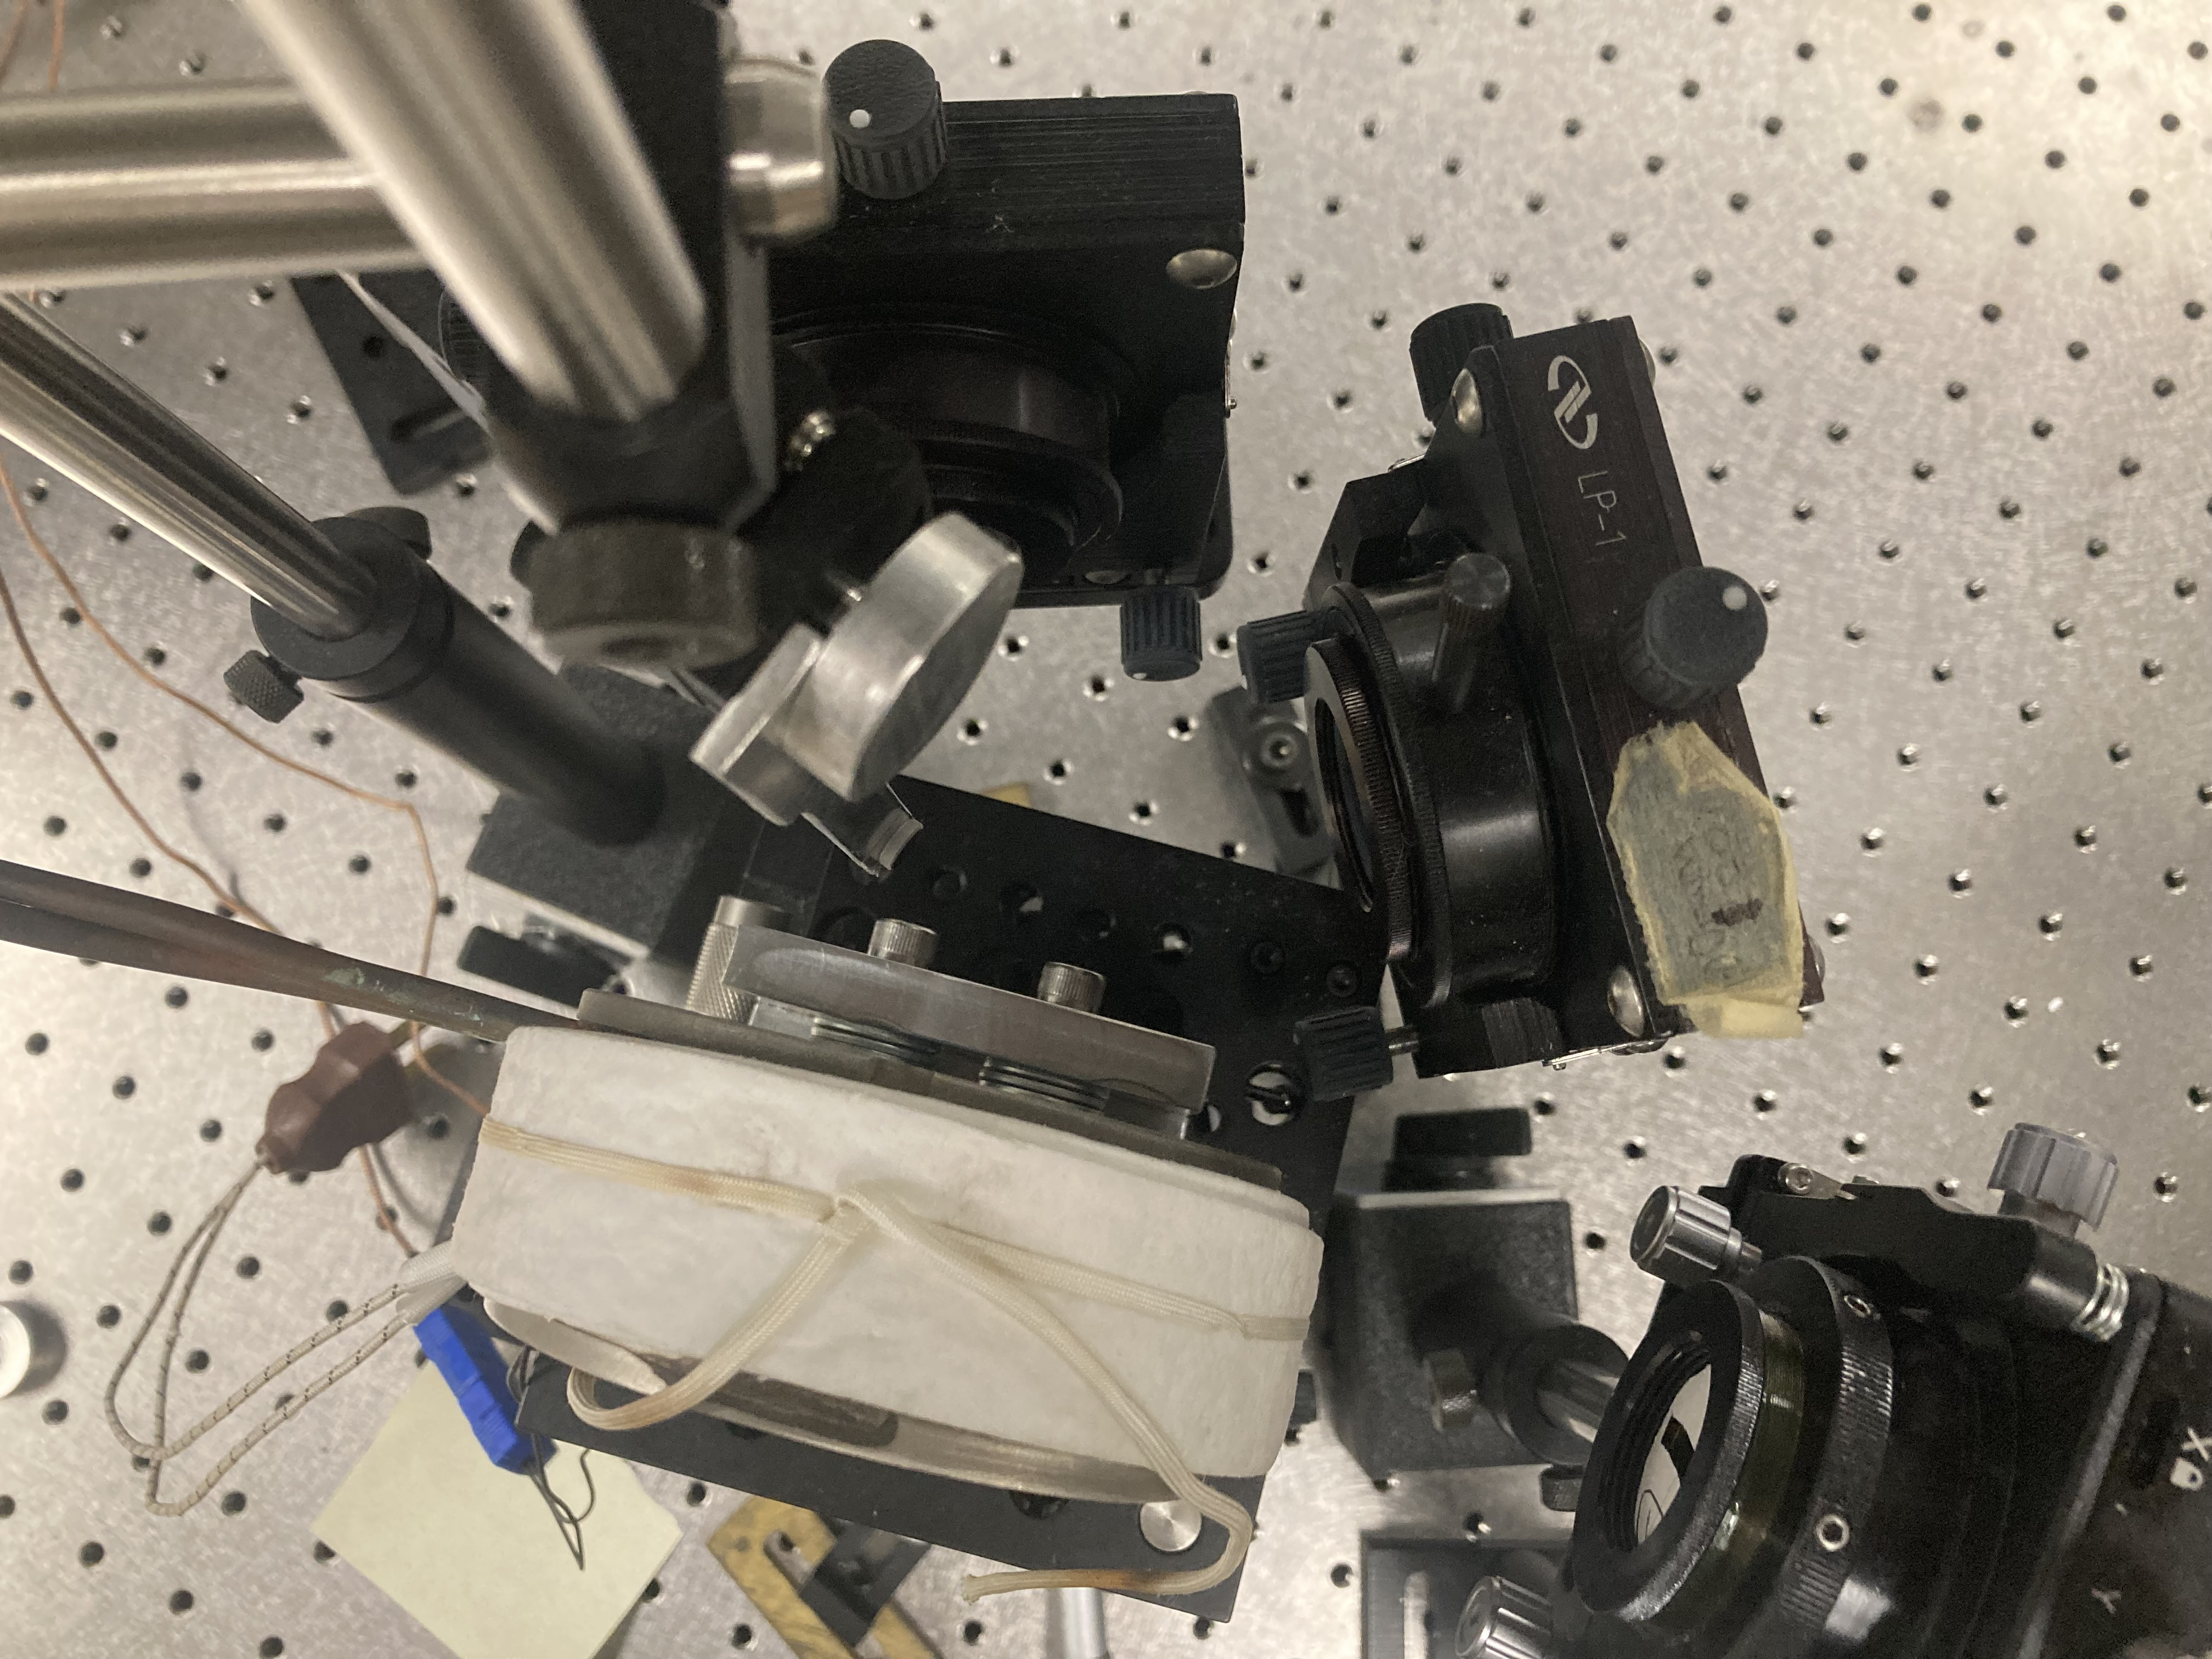
\includegraphics[width=0.45\textwidth]{IMG_1619.jpeg}};
		
		% Right image (shifted right)
		\node[anchor=south west, inner sep=0] (img2) at (0.5\textwidth,0)
		{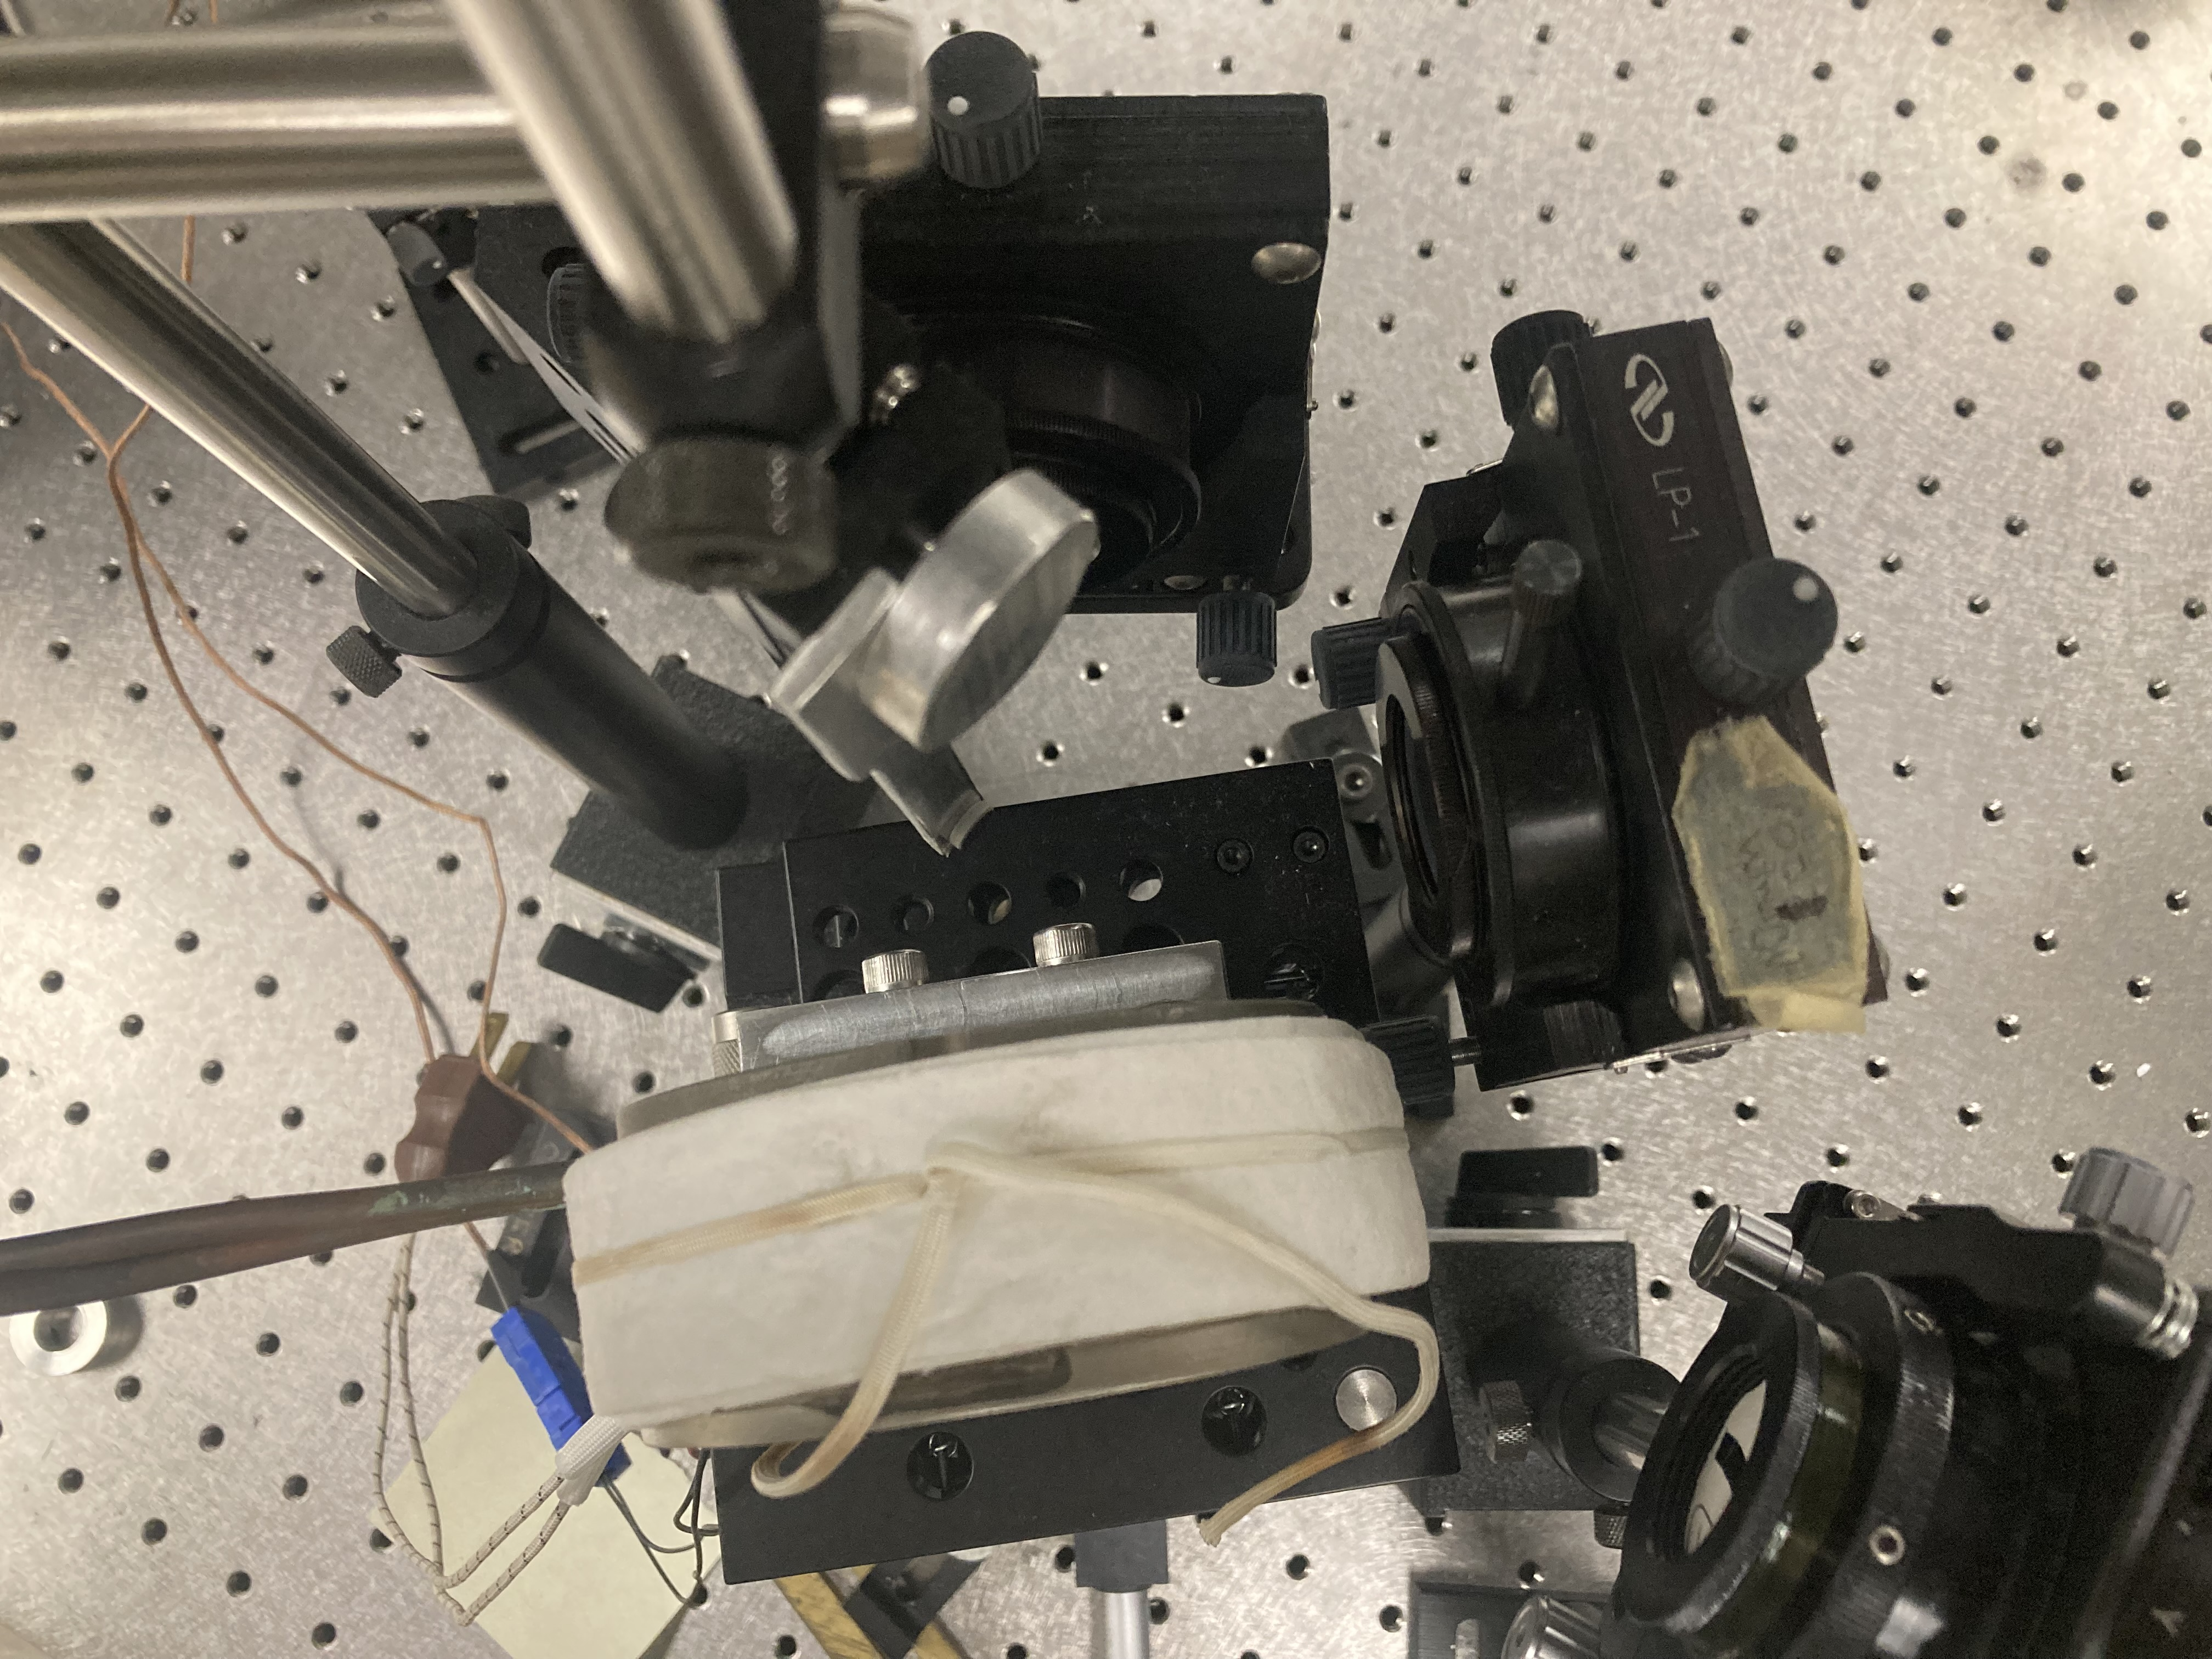
\includegraphics[width=0.45\textwidth]{IMG_1620.jpeg}};
		
		% Overlay for left image
		\begin{scope}[
			shift={(img1.south west)},
			x={($(img1.south east)-(img1.south west)$)},
			y={($(img1.north west)-(img1.south west)$)}
			]
			% draw on IMG_1619 here
			\draw[green, very thick,<-] (.42,0) -- (.42,1);
			\draw[green, thick] (.42,.25) -- (.41,.483);
			\draw[green, thick,->] (.41,.483) --(1,.6);
			
			\fill[green!60!black, opacity=0.25]
			(0.42,0.25) -- (0.6,1) -- (0.8,1) -- cycle;
			\draw[green!60!black, line width=0.5pt]
			(0.42,0.25) -- (0.6,1);
			\draw[green!60!black, line width=0.5pt]
			(0.42,0.25) -- (0.8,1);
			
			\node[red] at (0.2,0.45) {(BSM)};
			\draw[red,thick,->] (.28,.46) -- (.38,.481);
			
			\node[red] at (.32,0.25) {(DAC)};
			\node[red] at (.5,0.90) {(FO)};
			\node[red] at (.7,0.6) {(CO)};
		\end{scope}
		
		% Overlay for right image
		\begin{scope}[
			shift={($(img2.south west)+(0.25,0.08)$)},
			x={($(img2.south east)-(img2.south west)$)},
			y={($(img2.north west)-(img2.south west)$)}
			]
			
			% draw on IMG_1620 here
			\draw[green, very thick,<-] (.42,-0.01) -- (.42,.985);
			\draw[green, thick] (.42,.25) -- (.41,.483);
			\draw[green, thick,->] (.41,.483) --(.96,.6);
			
			\fill[green!60!black, opacity=0.25]
			(0.42,0.25) -- (0.2,.985) -- (0.4,.985) -- cycle;
			\draw[green!60!black, line width=0.5pt]
			(0.42,0.25) -- (0.2,.985);
			\draw[green!60!black, line width=0.5pt]
			(0.42,0.25) -- (0.4,.985);
		\end{scope}
		
	\end{tikzpicture}
	\caption{Optical geometry of the DAC assembly illustrating the role of specular reflections. In the left panel, the diamond anvil cell (DAC) is oriented to reject specular reflections from the diamond and gasket interfaces, minimizing the amount of reflected light collected by the detection optics. The shaded green conical region represents the angular distribution of this specular ``splash.'' The labeled components are the focusing optic (FO), collection optic (CO), back-scatter mirror (BSM), and diamond anvil cell (DAC). In the right panel, the DAC is intentionally rotated to direct this specular reflection onto the BSM, providing a local oscillator for heterodyne data acquisition.}
	\label{figure:DACStage}
\end{figure}

The solution was to invert the procedure of Herbst \etal: rather than rotating the DAC to reduce specular reflections, we incrementally rotated it to increase the amount of reflected light impinging on the collection optics, thereby providing a local oscillator of increasing intensity. The diamond anvil cell (DAC) is mounted on a precision translation and rotation stage, allowing for fine control of the scattering geometry. A representative view of the DAC mounted on the assembly stage is shown in \fig \ref{figure:DACStage}, illustrating the physical arrangement of the cell and the approximate scattering geometry used in this work.  

Successful heterodyne detection requires that the local oscillator and the scattered field traverse optical paths that are as nearly identical as practicable prior to mixing at the detector in order to assure a stable phase relationship. Utilizing spectrally reflected light from the diamond culets and gasket interfaces as the local oscillator naturally satisfies this requirement, as both the scattered and reflected fields originate within the same confined DAC geometry and propagate through essentially the same optical elements. Consequently, any difference in optical path length is limited to at most a small fraction of the culet separation ($\leq 100\,\si{\micro\meter}$), ensuring adequate phase coherence at the detector.  Correlation functions were obtained at a fixed pressure and temperature while incrementally increasing the angle subtended between the DAC and the incoming laser beam. The results are summarized in \tbl \ref{table:HetHomo}.  

\begin{table}[!htbp]
	\centering
	
	\tabletitle{PMT counts and relaxation times vs. DAC angle}
	\label{table:HetHomo}
	
	\begin{tabular}{lccc}
		\hline
		Angle (degrees) & Counts (thousands) & $\langle \tau \rangle$ ($\mu$s) & $\Delta \langle \tau \rangle$ ($\mu$s) \\
		\hline
		0  & 200 & 1360 & 54  \\
		5  & 164 & 1188 & 57  \\
		10 & 156 & 1296 & 73  \\
		15 & 120 & 1232 & 33  \\
		20 & 250 & 1449 & 57  \\
		\hline
	\end{tabular}
	
	\tabledescription{PMT count rates (in thousands) and corresponding $\alpha$-relaxation times $\langle \tau \rangle$ are shown as a function of DAC orientation. Zero degrees corresponds to the incoming laser at normal incidence to the diamond table; the DAC was then rotated \textit{toward} the collection mirror. The angular position was set using a calibrated rotation stage with an estimated uncertainty of $\pm 1^\circ$. The reported uncertainties $\Delta \langle \tau \rangle$ correspond to one-standard-deviation errors obtained from the covariance matrix of the nonlinear least-squares fits to the Cole--Davidson model.}
\end{table}

What is of primary interest here is how the expectation value of the relaxation time changes with increasing intensity of any heterodyne component. It is reasonable to assume that the intensity of light scattered directly from the sample is not substantially increased simply by rotating the DAC twenty degrees. Thus, the observed increase in PMT counts at certain angular positions must arise predominantly from additional scatter and specular reflections originating from the sources previously discussed.  

Although \fig \ref{figure:HetHomo} does appear to suggest an increasing trend in $\langle \tau \rangle$ as the heterodyne component is enhanced, it should be emphasized that the PMT counts more than double. As a bare minimum, then, the intensity of the local oscillator has been doubled, yet this corresponds to only a $\sim$17\% increase in $\langle \tau \rangle$. This outcome implies that the experiment is operating near, though perhaps not fully within, the heterodyne regime. We will later find the assumption that we are effectively within the heterodyne regime consistent with dynamic data obtained via other probes, including Brillouin scattering, \tgp, \etc

\begin{figure}[!htbp]
	\centering
	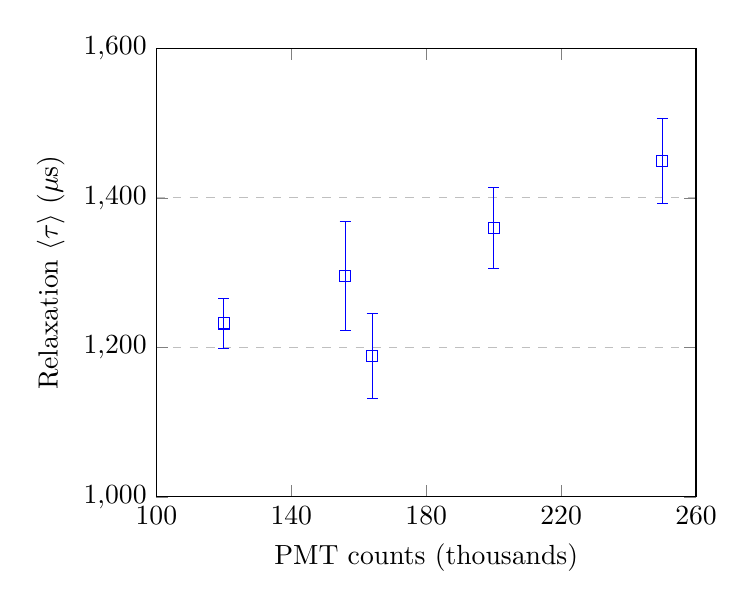
\begin{tikzpicture} 
		\begin{axis}[
			ylabel={Relaxation $\langle \tau \rangle$ ($\mu$s)},
			xlabel={PMT counts (thousands)},
			xmin=100, xmax=260,
			ymin=1000, ymax=1600,
			xtick={100,140,180,220,260},
			ytick={1000,1200,1400,1600},
			ymajorgrids=true,
			grid style=dashed,
			]
			\addplot+[only marks, mark=square, error bars/.cd, y dir=both, y explicit]
			coordinates { 
				(200,1360) +- (0,54) 
				(164,1188) +- (0,57) 
				(156,1296) +- (0,73) 
				(120,1232) +- (0,33) 
				(250,1449) +- (0,57) };
		\end{axis} 
	\end{tikzpicture}
	\caption{Structural relaxation times $\langle \tau \rangle$ as a function of increasing scatter and specular reflections serving as a local oscillator. Error bars represent 95\% confidence intervals derived from the mean square error (MSE) of the fit parameter $\tau$.}
	\label{figure:HetHomo}
\end{figure}

\subsection{Time-Correlation Functions}
\label{sec:TimeCorrelation}

The correlation spectra arising from the Brownian motion of mono-disperse colloidal spheres suspended in a liquid provide a useful point of reference from which to discuss our choice of time-correlation function adopted in this work. Consider the case of mono-disperse polystyrene spheres in methanol within the context of photon correlation spectroscopy experiments like those of Herbst \etal These spheres undergo diffusive motion in a relatively simple energy landscape. The resulting autocorrelation function exhibits a single-exponential decay, characterized by a well-defined relaxation time $\tau$ associated with translational diffusion.

By contrast, a typical glass-forming liquid exhibits a broad distribution of relaxation times. This distribution may arise from spatial heterogeneity, where different local environments relax at different rates, or from the presence of distinct relaxation modes within the system, and in practice may reflect a combination of both effects. Unlike the simple diffusive case described above, the corresponding time-correlation functions are no longer single exponential decays. Historically, these correlation data have been fit to the Kohlrausch--Williams--Watts (KWW) function \cite{Cardona2007,Williams}, which takes the form given in \eqn \ref{eqn:KWW}. When interpreted as a normalized time-correlation function, this may be written as
\begin{equation}
	C(t) = e^{-(t/\tau_{ww})^{\beta_{ww}}}, \quad 0 < \beta_{ww} \le 1.
	\label{eqn:KWWcorr}
\end{equation}
\noindent Here, $\tau_{ww}$ is a characteristic relaxation time and $\beta_{ww}$ quantifies the degree of stretching relative to a simple exponential decay.

In light scattering experiments, the fundamental observable is the dynamic structure factor $S(\vec q,\omega)$, which is related to the underlying correlation function through a Fourier transform:
\begin{equation}
	S(\vec q,\omega) = \mathscr{F}\!\left[ C(\vec q,t) \right].
	\label{eqn:SqwFromC}
\end{equation}
Thus, the spectral shape measured in frequency-domain techniques such as Brillouin light scattering reflects the frequency content of the relaxation dynamics encoded in $C(t)$. In time-domain techniques such as depolarized photon--correlation spectroscopy (DPCS), $C(t)$ is measured somewhat more directly.

The use of the KWW function to describe glassy systems is theoretically compelling for many reasons, not the least of which is that it captures the broad distribution of relaxation times characteristic of heterogeneous dynamics. Although often introduced in the context of dielectric spectroscopy—where the Laplace transform of the time derivative of $C(t)$ is related to the complex dielectric constant $\varepsilon^*$ as shown in \eqn \ref{eqn:delcTrans}—this reflects largely historical convention. Light scattering instead probes spatiotemporal fluctuations of the susceptibility tensor, $\delta\chi_{ij}(\mathbf r,t)$, which are directly related to fluctuations in the dielectric tensor. Consequently, both dielectric and light scattering measurements arise from the same underlying dielectric susceptibility tensor; however, light scattering probes the stochastic temporal evolution of its thermal fluctuations, whereas dielectric spectroscopy measures its response to an externally applied field:
\begin{equation}
	\frac{\varepsilon^{*} - \varepsilon_{\infty}}{\varepsilon_{0} - \varepsilon_{\infty}}
	= \mathscr{L}\!\left[ -\frac{\mathrm{d}C(t)}{\mathrm{d}t} \right]
	\label{eqn:delcTrans}
\end{equation}

Importantly, \eqn \ref{eqn:SqwFromC} and \eqn \ref{eqn:delcTrans} remain valid for arbitrary normalized relaxation functions, corresponding to any distribution of relaxation pathways and associated relaxation times\textemdash certainly including both KWW and Cole--Davidson forms described in \sect \ref{sec:models}. In the special case where $\beta = 1$, \eqn\ref{eqn:KWWcorr} reduces to a single exponential decay, corresponding to a Debye relaxation governed by a single characteristic timescale as with the Brownian motion of mono-disperse spherical particles in methanol studied by Herbst \etal \cite{Herbst}. Here the dynamics arise from random momentum transfer due to continual collisions with surrounding solvent molecules. Under these conditions, the system exhibits a well-defined relaxation time set by viscous dissipation and thermal fluctuations, leading to a correlation function characterized by a single timescale $\tau$. The corresponding dynamic structure factor of \eqn \ref{eqn:SqwFromC} then assumes the familiar Lorentzian form in frequency space,
\begin{equation}
	S(\vec q,\omega) \propto \frac{1}{1 + (\omega \tau)^2}.
	\label{eqn:debye_scattering}
\end{equation}

When working in frequency space, such as with Brillouin light scattering or dielectric frequency-response analysis, the relaxation dynamics of glass-forming systems are often described by functional forms such as the Cole--Davidson function of \eqn \ref{eqn:ColeDavidson} which, despite initial appearances, is closely analogous to \eqn \ref{eqn:KWW}. Both equations lend themselves well to fitting the structural relaxation dynamics of glass forming liquids.  In Brillouin light scattering, the spectral shape of the dynamic structure factor is often described phenomenologically by
\begin{equation}
	S(\vec q,\omega) \propto \Re\!\left[
	\left( \frac{1}{1 + i \omega \tau_{\mathrm{CD}}} \right)^{\beta_{\mathrm{CD}}}
	\right],
	\label{eqn:CD_Sqw}
\end{equation}
\noindent which, for $\beta_{\mathrm{CD}}=1$ reduces to 
\begin{equation}
	S(\vec q,\omega) \propto
	\Re\!\left[
	\frac{1}{1 + i \omega \tau}
	\right]
	=
	\frac{1}{1 + (\omega \tau)^2},
	\label{eqn:AlsoDebye}
\end{equation}
\noindent equivalent to \eqn \ref{eqn:debye_scattering} arising from the KWW model.

The equivalence of \eqn \ref{eqn:CD_Sqw} and \eqn \ref{eqn:KWWcorr} when both $\beta_{ww}=1$ and $\beta_{\mathrm{CD}}=1$ might suggest that the Cole--Davidson function is the Fourier transform of the KWW stretched exponential. It is not. Both functions may be interpreted as arising from a distribution of elementary relaxation processes, each independently describable by a simple exponential decay in the time domain. However, because they assume fundamentally different distribution functions, the extracted values of their respective $\tau$ and $\beta$ are not identical.

This discrepancy is not inconsequential, since multiple probes, operating in both the frequency and time domains, are required to track molecular dynamics in glass-forming systems across an enormous dynamic range. In this study, we would like to fit time domain DPCS data to a Cole--Davidson distribution to assure direct comparability with Brillouin data taken in the frequency regime. Lindsey and Patterson made this possible\nolinebreak\cite{Lindsey}\textemdash relating these two models by explicitly assuming that the KWW and Cole--Davidson functions arise from distributions of simple exponential decays, as follows:

\begin{equation}e^{-(t/\tau_{\mathrm{KWW}})^{\beta}}= \int_{0}^{\infty} e^{-t/\tau}\rho_{\mathrm{KWW}}(\tau)\mathrm{d}\tau
\end{equation}

\noindent and

\begin{equation}\left( \frac{1}{1+i\omega\tau_{\mathrm{CD}}} \right)^{\beta_{\mathrm{CD}}}= \int_{0}^{\infty} \frac{1}{\tau}\left( \frac{1}{1+i\omega\tau} \right)\rho_{\mathrm{CD}}(\tau)\mathrm{d}\tau.
	\label{eqn:distCD}
\end{equation}

A great deal of effort was devoted to solving for these distributions, $\rho_{\mathrm{CD}}$ and $\rho_{\mathrm{KWW}}$. Lindsey and Patterson provided an explicit form for $\rho_{\mathrm{CD}}(\tau)$, given by

\begin{equation}\label{eqn}\rho_{\mathrm{CD}}(\tau) =\frac{\sin(\pi \beta_{\mathrm{CD}})}{\pi}\left( \frac{\tau}{\tau_{\mathrm{CD}} - \tau} \right)^{\beta_{\mathrm{CD}}}.\end{equation}

\noindent This distribution, obtained from \eqn \ref{eqn:distCD} together with the normalization condition

\begin{equation}\int_{0}^{\infty} \frac{1}{\tau}\rho_{\mathrm{CD}}(\tau)\mathrm{d}\tau = 1,
\end{equation}

\noindent allows one to define the Cole–Davidson function in the time domain. Recall that $\rho_{\mathrm{CD}}(\tau)$ was derived under the assumption that the Cole–Davidson form corresponds to a distribution of simple Debye processes.  The Cole–Davidson function can be written in the time domain as

\begin{equation}
	\left( \frac{1}{1 + i \omega \tau_{\mathrm{CD}}} \right)^{\beta_{\mathrm{CD}}}= \mathscr{L}\left[ -\frac{\mathrm{d}}{\mathrm{d}t}\int_{0}^{\tau_{\mathrm{CD}}} \frac{1}{\tau}e^{-t/\tau}\rho_{\mathrm{CD}}(\tau)\mathrm{d}\tau \right].
\end{equation}

The work of Lindsey and Patterson has been available for four decades, yet it is clear why it became common practice to fit time-domain data to a KWW stretched exponential and then convert the parameters, rather than fitting directly to the Cole–Davidson distribution. Requiring a nonlinear fit routine to perform this integration would have been prohibitively resource-intensive on 1980s hardware. It remains nontrivial even today, though it can be recast into a form involving one- and two-parameter Gamma functions which, with the aid of modern lookup tables, can be evaluated relatively efficiently as follows in \eqn \ref{eqn:timeColeDavidson}.

\begin{equation}
	\int_{0}^{\tau_{\mathrm{CD}}} \frac{1}{\tau}e^{-t/\tau}\rho_{\mathrm{CD}}(\tau)\mathrm{d}\tau= \frac{1}{\pi}\Gamma\left(1-\beta_{\mathrm{CD}}\right)\Gamma\left(\beta_{\mathrm{CD}}, \tfrac{t}{\tau_{\mathrm{CD}}}\right)\sin\left(\pi\beta_{\mathrm{CD}}\right)
	\label{eqn:timeColeDavidson}
\end{equation}

Thus, in order to obtain values of $\tau$ that are directly comparable to those derived from frequency-domain Brillouin studies, all DPCS time-domain correlation decays will be fit in \textit{Mathematica} to a distribution of single-exponential decays corresponding to a Cole–Davidson function in the frequency domain, as expressed in \eqn \ref{eqn:DPCS}.

\begin{equation}
	C_{\mathrm{CD}}(t) =\frac{1}{\pi}\Gamma\left(1-\beta_{\mathrm{CD}}\right)\Gamma\left(\beta_{\mathrm{CD}}, \tfrac{t}{\tau_{\mathrm{CD}}}\right)\sin\left(\pi \beta_{\mathrm{CD}}\right)
	\label{eqn:DPCS}
	\end{equation}

\section{Autocorrelation Data Analysis and Fitting Methodology}
\label{sec:DAC75CExample}

The sequence of experimentally determined autocorrelation functions presented in \fig \ref{fig:PCS75CRegression} is taken from the 75~\textdegree C isothermal cumene data covering a pressure range from 20.0 to 27.8 kbar, over which the structural relaxation time fits within the eight- to nine-decade time window of PCS. As noted previously in \sect \ref{sec:PCSExp}, autocorrelations obtained in a DAC are not expected to be as tidy as those from conventional cuvette geometries. Two experimental realities dominate the appearance of these data. First, microscopic impurities, gasket scatter, and dust create significant background scattering not associated with the liquid dynamics. At lower temperatures (or higher pressures) these larger scatterers are effectively immobile on our timescales and, along with spectral reflections, will tend the experiment towards the heterodyne regime. Under thermodynamic conditions for which $\tau_\alpha$ is sufficiently small, some of these particles become mobile on experimental timescales. When such a particle enters or leaves the scattering volume mid-acquisition, the baseline of the autocorrelation can swing substantially and may take impractically long to average back to a flat baseline.

\begin{figure}[!htbp]
	\centering
	\begin{tikzpicture}
		\begin{axis}[
			xlabel={Seconds},
			ylabel={Normalized Autocorrelation [$g_{2}(t)$]},
			title={\shortstack{Depolarized Photon Correlation Spectroscopy \\of Cumene at 75 °C}},
			grid=both,
			xmode=log,     
			xticklabel style={rotate=45, anchor=east}, 
			transpose legend,       
			legend pos=north east,
			legend columns=5,
			width=12cm, height=8cm
			]
			
			% 20.0 kbar (blue filled)
			\addplot[only marks, mark=*, mark size=1pt, color=blue, fill=blue] 
			table[col sep=comma, x={20_0kbar xd}, y={20_0kbar yd}] {Chapters/PCS/Figures/data.csv};
			\addlegendentry{\SI{20.0}{\kilo\bar}}
			\addplot[semithick, color=red, forget plot]
			table[col sep=comma, x={20_0kbar xf}, y={20_0kbar yf}] {Chapters/PCS/Figures/data.csv};
			
			% 21.5 kbar (orange open)
			\addplot[only marks, mark=o, mark size=1pt, color=orange] 
			table[col sep=comma, x={21_21kbar xd}, y={21_21kbar yd}] {Chapters/PCS/Figures/data.csv};
			\addlegendentry{\SI{21.5}{\kilo\bar}}
			\addplot[semithick, color=red, forget plot]
			table[col sep=comma, x={21_21kbar xf}, y={21_21kbar yf}] {Chapters/PCS/Figures/data.csv};
			
			% 22.1 kbar (green filled)
			\addplot[only marks, mark=triangle*, mark size=1.2pt, color=green, fill=green] 
			table[col sep=comma, x={22_06kbar xd}, y={22_06kbar yd}] {Chapters/PCS/Figures/data.csv};
			\addlegendentry{\SI{22.1}{\kilo\bar}}
			\addplot[semithick, color=red, forget plot]
			table[col sep=comma, x={22_06kbar xf}, y={22_06kbar yf}] {Chapters/PCS/Figures/data.csv};
			
			% 23.1 kbar (purple open)
			\addplot[only marks, mark=triangle, mark size=1.2pt, color=purple] 
			table[col sep=comma, x={23_14kbar xd}, y={23_14kbar yd}] {Chapters/PCS/Figures/data.csv};
			\addlegendentry{\SI{23.1}{\kilo\bar}}
			\addplot[semithick, color=red, forget plot]
			table[col sep=comma, x={23_14kbar xf}, y={23_14kbar yf}] {Chapters/PCS/Figures/data.csv};
			
			% 24.0 kbar (black open)
			\addplot[only marks, mark=square, mark size=1pt, color=teal] 
			table[col sep=comma, x={24_0kbar xd}, y={24_0kbar yd}] {Chapters/PCS/Figures/data.csv};
			\addlegendentry{\SI{24.0}{\kilo\bar}}
			\addplot[semithick, color=red, forget plot]
			table[col sep=comma, x={24_0kbar xf}, y={24_0kbar yf}] {Chapters/PCS/Figures/data.csv};
			
			% 24.9 kbar (blue filled again — cycle restarts)
			\addplot[only marks, mark=diamond*, mark size=1.2pt, color=blue, fill=blue] 
			table[col sep=comma, x={24_92kbar xd}, y={24_92kbar yd}] {Chapters/PCS/Figures/data.csv};
			\addlegendentry{\SI{24.9}{\kilo\bar}}
			\addplot[semithick, color=red, forget plot]
			table[col sep=comma, x={24_92kbar xf}, y={24_92kbar yf}] {Chapters/PCS/Figures/data.csv};
			
			% 25.2 kbar (orange open again)
			\addplot[only marks, mark=diamond, mark size=1.2pt, color=orange] 
			table[col sep=comma, x={25_2kbar xd}, y={25_2kbar yd}] {Chapters/PCS/Figures/data.csv};
			\addlegendentry{\SI{25.2}{\kilo\bar}}
			\addplot[semithick, color=red, forget plot]
			table[col sep=comma, x={25_2kbar xf}, y={25_2kbar yf}] {Chapters/PCS/Figures/data.csv};
			
			% 26.4 kbar (green filled again)
			\addplot[only marks, mark=pentagon*, mark size=1.3pt, color=green, fill=green] 
			table[col sep=comma, x={26_43kbar xd}, y={26_43kbar yd}] {Chapters/PCS/Figures/data.csv};
			\addlegendentry{\SI{26.4}{\kilo\bar}}
			\addplot[semithick, color=red, forget plot]
			table[col sep=comma, x={26_43kbar xf}, y={26_43kbar yf}] {Chapters/PCS/Figures/data.csv};
			
			% 26.8 kbar (purple open again)
			\addplot[only marks, mark=pentagon, mark size=1.3pt, color=purple] 
			table[col sep=comma, x={26_8kbar xd}, y={26_8kbar yd}] {Chapters/PCS/Figures/data.csv};
			\addlegendentry{\SI{26.8}{\kilo\bar}}
			\addplot[semithick, color=red, forget plot]
			table[col sep=comma, x={26_8kbar xf}, y={26_8kbar yf}] {Chapters/PCS/Figures/data.csv};
			
			% 27.8 kbar (teal filled again)
			\addplot[only marks, mark=star, mark size=1.3pt, color=teal, fill=teal] 
			table[col sep=comma, x={27_8kbar xd}, y={27_8kbar yd}] {Chapters/PCS/Figures/data.csv};
			\addlegendentry{\SI{27.8}{\kilo\bar}}
			\addplot[semithick, color=red, forget plot]
			table[col sep=comma, x={27_8kbar xf}, y={27_8kbar yf}] {Chapters/PCS/Figures/data.csv};
			
		\end{axis}
	\end{tikzpicture}
	\caption{DPCS autocorrelations of cumene measured in a DAC at 75~\textdegree C across a range of pressures over which $\tau_\alpha$ fits within the time window of our autocorrelator. The sequence highlights two dominant elevated-temperature artifacts: slowly varying baseline offsets and photon-limited short-lag noise. Mitigation and fitting strategy are discussed in the text.}
	\label{fig:PCS75CRegression}
\end{figure}

This fluctuating baseline is shown in \fig \ref{fig:PCS75CBaseline} for one of our higher-pressure datapoints\textemdash 26.8 kbar. It should be noted that these are not taken at set time intervals but are instead the result of periodically saving the acquisitions during long runs; one never knows when a severe baseline fluctuation may render the data unfittable, so earlier saved autocorrelations can preserve a data point that often required hours, if not days, to obtain.

It may also be seen from \fig \ref{fig:PCS75CBaseline} that the first autocorrelation was saved relatively early, before the decay had fully converged to the actual relaxation\textemdash \ie, it lies well above the regressions saved at later times. However, all of the subsequent regressions quickly converge, as was typical for all acquisitions, even though the baseline at high pressures and temperatures very rarely does so for the aforementioned reasons.


\begin{figure}[!htbp]
	\centering
	\begin{tikzpicture}
		\begin{axis}[
			xlabel={Seconds},
			ylabel={Normalized Autocorrelation [$g_{2}(t)$]},
			title={Baseline Instability in DAC for Cumene at 75 °C},
			grid=both,
			xmode=log,     
			xticklabel style={rotate=45, anchor=east}, 
			transpose legend, 
			legend cell align=left,      
			legend pos=north east,
			legend columns=1,
			width=12cm, height=8cm
			]
			
			% t=1
			\addplot[only marks, mark=*, mark size=1pt, color=gray, fill=gray] 
			table[col sep=comma, x={x15nv04_1}, y={y15nv04_1}] {Chapters/PCS/Figures/data.csv};
			\addlegendentry{First};
			
			% t=2
			\addplot[only marks, mark=o, mark size=1pt, color=orange, fill=orange] 
			table[col sep=comma, x={x15nv04_2}, y={y15nv04_2}] {Chapters/PCS/Figures/data.csv};
			\addlegendentry{Second};
			
			% t=3
			\addplot[only marks, mark=triangle*, mark size=1pt, color=green, fill=green] 
			table[col sep=comma, x={x15nv04_3}, y={y15nv04_3}] {Chapters/PCS/Figures/data.csv};
			\addlegendentry{Third};
			
			% t=4
			\addplot[only marks, mark=triangle*, mark size=1pt, color=purple, fill=purple] 
			table[col sep=comma, x={x15nv04_4}, y={y15nv04_4}] {Chapters/PCS/Figures/data.csv};
			\addlegendentry{Fourth};
			
			% t=5
			\addplot[only marks, mark=square, mark size=1pt, color=teal, fill=teal] 
			table[col sep=comma, x={x15nv04_5}, y={y15nv04_5}] {Chapters/PCS/Figures/data.csv};
			\addlegendentry{Fifth};
			
			% t=6
			\addplot[only marks, mark=diamond*, mark size=1pt, color=blue, fill=blue] 
			table[col sep=comma, x={x15nv04_6}, y={y15nv04_6}] {Chapters/PCS/Figures/data.csv};
			\addlegendentry{Sixth};
					
		\end{axis}
	\end{tikzpicture}
	\caption{Autocorrelations of cumene at 75~\textdegree C and $26.8$ kbar illustrating the fluctuating baselines characteristic of DAC measurements under thermodynamic conditions such that mobile contaminants interfere with data analysis. Each curve represents a saved acquisition taken at a different time during the run. The earliest save (``First'') was recorded before the decay had fully converged to the true relaxation and therefore lies well above the later regressions. Subsequent saves converge rapidly to a consistent relaxation profile, while the overall baseline remains unstable likely due to mobile impurities entering or leaving the scattering volume mid-acquisition.}
	
	\label{fig:PCS75CBaseline}
\end{figure}

An additional consideration is that the DAC severely limits the illuminated/scattering volume. Scattering volumes typical for PCS in a cuvette are often on the order of hundreds of nanoliters. However, because the culets of the DAC constrain the length of the scattering column, often to 100 microns or less, the effective scattering volume may be reduced by two orders of magnitude or more to that which is common in a more classical cuvette-centered experimental setup. For the fastest autocorrelation channels this often implies $\ll 1$ photon per scan on average, so the short-lag-time ``head'' of the normalized autocorrelation function $g_{2}(t)$ is photon-shot-noise dominated. This gives rise to the poorly defined low-lag region shown in \fig \ref{fig:PCS75CHead}. Unlike baseline drift, this head noise persists even at relatively low temperatures or high pressures, as it originates from photon statistics within a tiny scattering volume. At lower temperatures or higher pressures, however, the intrinsic dynamics are much slower, and the shot noise inherent to these fast channels becomes of little consequence. In fact, it is quite common for the autocorrelation curve to lack a head entirely at high temperatures or low pressures where the liquid's structural relaxation time lies beyond or just outside the range of the correlator's fastest channels. This behavior is clearly visible in the data presented in \fig \ref{fig:PCS75CRegression}, taken at 22.1 kbar and 75~\textdegree C.

 
\begin{figure}[!htbp]
	\centering
	\begin{tikzpicture}
		\begin{axis}[
			xlabel={Seconds},
			ylabel={Normalized Autocorrelation [$g_{2}(t)$]},
			title={\shortstack{Photon Shot-Noise--Dominated Short-Lag Region\\in DAC for Cumene at 75 °C}},
			grid=both,
			xmode=log,     
			xticklabel style={rotate=45, anchor=east}, 
			xmax=.01,
			transpose legend,  
			legend cell align=left,      
			legend pos=north east,
			legend columns=1,
			width=12cm, height=8cm
			]
			
			\addplot[only marks, mark=*, mark size=1pt, color=blue, fill=blue] 
			table[col sep=comma, x={22_06kbar xd}, y={22_06kbar yd}] {Chapters/PCS/Figures/data.csv};
			\addlegendentry{\SI{22.1}{\kilo\bar}}
			
			\addplot[mark=none, color=red] 
			table[col sep=comma, x={22_06kbar xf}, y={22_06kbar yf}] {Chapters/PCS/Figures/data.csv};
			\addlegendentry{Cole-Davidson fit}
			
		\end{axis}
	\end{tikzpicture}
	\caption{Autocorrelation of cumene at 75\textdegree C and \SI{22.1}{\kilo\bar} illustrating the shot-noise–dominated short-lag region that arises from the severely reduced scattering volume in the DAC.}
	
	
	\label{fig:PCS75CHead}
\end{figure}

Despite these complications being more pronounced at higher temperatures, the 75~\textdegree C data series is included here as it represents the “worst-case’’ data quality we encountered and thus motivates the regression fit strategy outlined below which has been implemented here to extract reliable relaxation times.

Obtaining robust Cole–Davidson fits in the time domain ideally requires well-defined heads and baselines. Of these, the baseline is often most critical given that, for the Cole-Davidson distribution, $\tau_{\mathrm{CD}}$ is the discrete upper cutoff of the structural-relaxation mode distribution. The expectation value satisfies $\langle \tau \rangle_{\mathrm{CD}}=\beta_{\mathrm{CD}}\,\tau_{\mathrm{CD}}$. In the DAC, especially at higher temperatures, a clean baseline can be unattainable, while at the fastest lags the head can be too noisy to anchor the early-time curvature due to shot noise. The practical remedy is therefore to constrain the shape parameter, $\beta_{\mathrm{CD}}$, or at least to establish a functional dependence of $\beta_{\mathrm{CD}}$ on pressure and temperature. Without such a constraint, the fit becomes underdetermined when either the head or baseline is unreliable. When a portion of the autocorrelation function must be excluded, whether the early-time head or the late-time baseline, fixing $\beta_{\mathrm{CD}}$ removes the principal degeneracy between amplitude and shape in the fit. This constraint allows $\tau_{\mathrm{CD}}$ to be determined primarily by the curvature of the mid-lag region. In practice, most datasets furnish at least one clean side, so constraining $\beta_{\mathrm{CD}}$ empirically or through a pressure-temperature-dependent model would ensure consistent $\tau_{\mathrm{CD}}$ values and hence consistent mean relaxation times $\langle \tau \rangle = \beta_{\mathrm{CD}}\tau_{\mathrm{CD}}$.

\begin{figure}[!htbp]
	\centering
	\begin{tikzpicture}
		\node[anchor=south west, inner sep=0] (img) at (0,0)
		{
\includegraphics[width=0.85\linewidth]{chapters/pcs/figures/Beta Analysis.JPG}};
		
		\begin{scope}[
			x={($(img.south east)-(img.south west)$)},
			y={($(img.north west)-(img.south west)$)}
			]
			% Cover old "DLS" label
			\fill[white] (0.835,0.35) rectangle (0.955,0.45);
			
			% Write corrected labels
			\node[anchor=west] at (0.835,0.425) {\fontsize{12}{11}\selectfont DBLS};
			\node[anchor=west] at (0.835,0.38) {\fontsize{12}{11}\selectfont DPCS};
		\end{scope}
	\end{tikzpicture}
	\caption{Pressure dependence of the Cole--Davidson shape parameter, $\beta_{\mathrm{CD}}$, obtained from depolarized Brillouin (black circles) and DPCS (green diamonds) measurements. Error bars represent $1\sigma$ uncertainties derived from the nonlinear fit covariance matrices. The inset shows the temperature dependence of $\beta_{\mathrm{CD}}$ at selected pressures, demonstrating its statistical invariance across a large experimental domain.}
	\label{fig:beta}
\end{figure}

As it happens, our lab has plenty of relaxation data at various pressures and temperatures for cumene in the form of depolarized Brillouin light-scattering data as well as DPCS.  The values for $\beta_{\mathrm{CD}}$ along with $1\sigma$ uncertainties derived from the covariance matrix of the nonlinear fits, is shown in \fig \ref{fig:beta}.  It is notable that the error bars for $\beta_{\mathrm{CD}}$ become excessively large near ambient pressure.  The larger uncertainties in the Brillouin fits at low pressure arise due to the structural–relaxation (Mountain) component becoming less distinct from the quasi-elastic background near the Bose peak, increasing parameter covariance in the Cole–Davidson fits.  However, as there was no evident trend in the value of $\beta_{\mathrm{CD}}$ approaching the Bose peak, there is no reason to believe such a trend would suddenly appear as we approach ambient pressure.  To extend this analysis, DPCS data was also included under conditions where an autocorrelation could be obtained having a solid low-lag head and baseline thus allowing for a nonlinear fit from which $\beta_{\mathrm{CD}}$ could be confidently obtained.  This is particularly compelling as it not only extends our analysis of the pressure dependence of $\beta_{\mathrm{CD}}$ up to nearly $2.5~\si{\giga\pascal}$, but also further assures us that our time-domain Cole-Davidson fits to our autocorrelations are returning the appropriate values for comparison with our frequency-domain data.  It is very evident that there is no significant pressure dependence in the value of $\beta_{\mathrm{CD}}$ from ambient pressure up to nearly $2.5~\si{\giga\pascal}$.

The inset plot of \fig \ref{fig:beta} is comprised entirely of DPCS autocorrelation fits where solid low-lag heads and baselines were obtainable.  It is clear that over the range of 40~$^\circ$C for which these data were obtained there is no significant temperature dependence in the value of  $\beta_{\mathrm{CD}}$.  Thus, we make the assumption that, for the glass former cumene, over the ranges of pressure and temperature here investigated, the value of  $\beta_{\mathrm{CD}}=0.509$.  This value is used consistently for all Cole-Davidson fits to cumene data here presented.

For internal validation, we applied this procedure to runs where both a clean head and a flat baseline are present. The full autocorrelation is first fit with $\{\tau_{\mathrm{CD}},\beta_{\mathrm{CD}}\}$ free to obtain $\tau_{\mathrm{CD}}^{(\text{full})}$ and $\beta_{\mathrm{CD}}^{(\text{full})}$. The analysis is then repeated twice: once with the short-lag head removed and $\beta_{\mathrm{CD}}=0.509$, and once with the baseline removed and the same fixed $\beta_{\mathrm{CD}}$. In both cases the recovered $\tau_{\mathrm{CD}}$ agrees with $\tau_{\mathrm{CD}}^{(\text{full})}$ within the 95\% confidence interval, indicating that a single reliable side of the decay suffices when $\beta_{\mathrm{CD}}$ is constrained. 


\section{Results and Discussion}\label{sec:result}
\subsection{Thermodynamic Scaling}\label{sec:tdscaling}

Another means of validating the DPCS data—and of confirming that the measurements were obtained under heterodyne or homodyne experimental conditions—is to examine how well they conform to the established thermodynamic scaling behavior of cumene \cite{RansomPRL}. The cumene \tgp data, provided here and in \app \ref{app:CumeneIGP}, allows us to determine the appropriate scaling factor.  

Liquids that obey thermodynamic scaling exhibit a relationship between temperature, volume, and relaxation time of the form:  
\begin{equation}\label{eqn:tdscaling}
	\tau \propto \frac{1}{T V^{\gamma}}
\end{equation}

\noindent Experimentally, the \tgp process provides the glass-transition temperature as a function of pressure. To proceed, it is necessary to convert these pressures to the corresponding specific volumes. For cumene, this conversion is carried out using the modified Tait equation of state provided in \app \ref{app:CumeneEOS}.  

Thus, since the \tgp data comprise an isochronous curve at $\tau \approx 100 \,\si{\second}$, taking the logarithm of both sides of \eqn \ref{eqn:tdscaling} yields the linear expression in \eqn \ref{eqn:lingamma}. The slope of this relation gives the scaling factor $\gamma$, while the $y$-intercept provides an estimate of the relaxation time associated with the \tgp data.  

\begin{equation}\label{eqn:lingamma}
	\log_{10}(T) = -\gamma \log_{10}(V) - \log_{10}(\tau_{G})
\end{equation}

\noindent The TGP data for cumene from \app \ref{app:CumeneIGP} are plotted as $\log_{10}(T_g)$ versus $\log_{10}(V_g)$ and indeed our data show a very linear relation.  A linear regression yields a value of the scaling exponent for cumene of 4.77 and an intercept of 2.11, from which we calculate an average relaxation time of tau = 130 s for Tg(P).

\begin{figure}[!htbp]
	\centering
	\begin{tikzpicture} 
		\begin{axis}[
			title={Scaling Parameter from \tgp Data},
			ylabel={$\log_{10} T_{G}$},
			xlabel={-$\log_{10} V_{G}$},
			ymin=2.1, ymax=2.7,
			xmin=0, xmax=0.12,
			xtick={0,0.04,0.08,0.12},
			ytick={2.1,2.3,2.5,2.7},
			]
			\addplot table [only marks, x=a, y=b, col sep=comma] {TDScaling.csv};
			\addplot {4.77*x + 2.1096};
		\end{axis}
		\node at (1.3,4.9) {$\gamma = 4.77$};
		\draw[black, thick] (.4,4.6) rectangle (2.1,5.3);
	\end{tikzpicture}
	\caption{Linearized cumene \tgp data from \app \ref{app:CumeneIGP} fit to the regression model $\log_{10}(T) = -\gamma \log_{10}(V) - \log_{10}(\tau_{G})$. The slope gives $\gamma = 4.79$, and the $y$-intercept of 2.11 corresponds to an average \tgp relaxation time of $\tau \approx 130 \,\si{\second}$.}
	\label{figure:tdscaling}
\end{figure}


The value of the scaling factor having been obtained in this fashion, the DPCS data provided in \app \ref{app:DPCSdata} may be checked to determine whether it scales consistently with the Brillouin fast-dynamics data and the \tgp data for $\gamma = 4.77$. The corresponding specific volumes are again obtained via \eqn \ref{eqn:CumeneTait}. The results of this thermodynamic scaling are presented in \fig  \ref{figure:scaling}.  

With respect to the heterodyne/homodyne considerations addressed in \sect \ref{sec:HomoHeto}, the majority of the data were collected with the DAC oriented such that a significant amount of local oscillator light from the surfaces was captured along with the desired signal, thereby ensuring that we were well within the heterodyne regime. These data were fit to \eqn \ref{eqn:DPCS} to obtain the $\alpha$-relaxation parameter, $\tau_{\mathrm{CD}}$. The scaled values are labeled “DPCS” in \fig  \ref{figure:scaling} and show excellent agreement with both the scaled Brillouin and \tgp data.  

Because the intensity of light scattered from the sample volume is so much weaker than that of the local oscillator, it was often necessary to signal average for several hours in the heterodyne configuration. As noted in \sect \ref{sec:HomoHeto}, it was generally assumed that the experiment always operated well within the heterodyne regime due to the exceedingly small sample volume. Thus, minimizing scatter from the DAC surfaces in order to reduce acquisition time seemed reasonable.  

With this in mind, when the 75\textdegree{} isotherm was measured, the DAC was oriented to minimize PMT counts. This resulted in relatively rapid acquisition—in some cases as little as ten minutes. However, when these data were fit to \eqn \ref{eqn:DPCS} and scaled, the resulting points systematically lay above the rest of the data known to be solidly heterodyne. This suggested that the measurement was perhaps closer to purely homodyne conditions than originally assumed.  

Lacking a reliable means of quantifying the degree of homodynicity, the data were instead fit to \eqn \ref{eqn:hetero}, which assumes a Cole–Davidson distribution of purely heterodyne correlation decays:  
\begin{equation}\label{eqn:hetero}
	\int_{0}^{\tau_{\mathrm{CD}}} \frac{1}{\tau} e^{-2t/\tau} \rho_{\mathrm{CD}}(\tau)\, d\tau
	= \frac{1}{\pi} \, \Gamma\!\left(1-\beta_{\mathrm{CD}}\right)\,
	\Gamma\!\left(\beta_{\mathrm{CD}}, \tfrac{2t}{\tau_{\mathrm{CD}}}\right)\,
	\sin\!\left(\pi \beta_{\mathrm{CD}}\right)
\end{equation}

When refit under the assumption of homodynicity, the scaled values were found to agree with the remainder of the scaled data. This indicates that by orienting the DAC to reject non‑target light as aggressively as possible, the experiment operated under nearly pure homodyne conditions. With further development—particularly for liquids with strong depolarized scattering—it may be feasible to run confidently in a homodyne configuration, thereby accelerating data acquisition. However, because the only reliable way to confirm reasonably homodyne conditions is to compare with data known to be heterodyne, we elected to intentionally orient the DAC so that sufficient splash from the surfaces was collected to ensure the data were solidly within the heterodyne regime during acquisition. This procedure was used for all data except the 75\textdegree{}C isotherm.

\begin{figure}[!htbp]
	\centering
	\begin{tikzpicture}
		\begin{axis}[
			title={Thermodynamic Scaling of Cumene: DPCS, Brillouin, and \tgp},
			xtick scale label code/.code={},
			xlabel={$(T V^{\gamma})^{-1}\;(\times 10^{-2})$},
			ylabel={$\log_{10}\!\big(\tau_{\mathrm{CD}}\big)$},
			xmin=0, xmax=0.010,
			ymin=0, ymax=16,
			xtick={0,0.002,0.004,0.006,0.008,0.010},
			ytick={0,2,4,6,8,10,12,14,16},
			grid=both,
			width=0.9\textwidth,
			legend pos=south east,
			legend cell align=left
			]
			% IGP (isochronal reference)
			\addplot+[only marks, mark=triangle*, mark options={scale=0.7}]
			table [x=a, y=b, col sep=comma] {DPCSscaletgp.csv};
			\addlegendentry{\scriptsize \tgp}
			
			% DPCS (heterodyne, main dataset)
			\addplot+[only marks, mark=square*, mark options={scale=0.7}]
			table [x=a, y=b, col sep=comma] {DPCSscale.csv};
			\addlegendentry{\scriptsize DPCS (heterodyne)}
			
			% DPCS (75°C, near-homodyne refit)
			\addplot+[only marks, mark=*, mark options={scale=0.6}]
			table [x=a, y=b, col sep=comma] {DPCSscaleHomo75.csv};
			\addlegendentry{\scriptsize DPCS (75\textdegree{}C, homodyne fit)}
			
			% Brillouin (fast dynamics scaled)
			\addplot+[only marks, mark=diamond*, mark options={scale=0.7}]
			table [x=a, y=b, col sep=comma] {DPCSscalefast.csv};
			\addlegendentry{\scriptsize Brillouin}
		\end{axis}
	\end{tikzpicture}
	\caption{Thermodynamic scaling of cumene showing $\log_{10}(\tau_{\mathrm{CD}})$ \vs $(T V^{\gamma})^{-1}$ using $\gamma$ determined from \tgp. DPCS data acquired under intentionally heterodyne conditions (squares) align with scaled Brillouin fast‑dynamics data (diamonds) and \tgp (triangles). The 75\textdegree{}C isotherm, acquired with the DAC oriented to minimize PMT counts, is consistent with the heterodyne data when refit assuming homodyne correlation decays (circles).}
	\label{figure:scaling}
\end{figure}


\subsection{Alpha Relaxation Dynamics}\label{sec:surface}

As discussed in \sect \ref{sec:HomoHeto} and \sect \ref{sec:TimeCorrelation}, the broader goal of this chapter is to establish DPCS within a DAC as a reliable probe of the structural $\alpha$-relaxation. The utility of time-domain correlation methods for glass-forming liquids was first demonstrated by Demoulin \etal, who showed that the Cole--Davidson distribution provides a robust description of broad, nonexponential relaxation in undercooled glycerol\nolinebreak\cite{Demoulin}. Later, Lindsey and Patterson established the correspondence between the Williams--Watts stretched exponential and the Cole--Davidson form, thereby providing a practical framework for translating between time-domain and frequency-domain probes\nolinebreak\cite{Lindsey}. Building on this foundation, we pool together DPCS, DBLS, and \tgp data to provide a comprehensive picture of the $\alpha$-relaxation dynamics of cumene, spanning timescales from picoseconds to hundreds of seconds, and extending to pressures in excess of $ 3\;\si{\giga\pascal}$
	
To obtain a full description of the relaxation dynamics of cumene over the entire experimental range, data obtained from DPCS, as well as DBLS and \tgp methods, have been pooled together to fill in as much of the dynamic space as possible. For an initial attempt, a surface fit of this dynamic data was performed using the Vogel–Tammann-Fulcher (VTF) equation,
\begin{equation}
	\ln(\tau)=\ln(\tau_{\infty}) +\frac{DT_{0}}{T-T_{0}},
	\label{eqn:VTF}
\end{equation}
where $\tau_{\infty}$ is the relaxation time in the high-temperature limit (assumed constant for all pressures), $T_{0}$ is the zero-mobility temperature at which the $\alpha$-relaxation time asymptotically diverges, and $D$ is the fragility parameter. A simple polynomial expansion as used by Ransom and Oliver to extend the Tate equation of state into high pressures can be analogously implemented to the VTF \eqn \cite{RansomPRL}. Such an expansion of $D$ and $T_{0}$ allows this classically temperature-dependent model to capture dynamics over a wide pressure range—from ambient conditions up to approximately $4.5\;\si{\giga\pascal}$ in this study. The resulting pressure-extended VTF model, and the values for these parameters obtained, are summarized in \eqn \ref{eqn:VTFsurface}.

\begin{equation}
	\label{eqn:VTFsurface}
	\begin{split}
		\:& H\left(T,P\right) = \log(\tau_{\infty}) +\frac{D(P)T_{0}(P)}{T-T_{0}(P)}\\
		&\text{with:}\\
		&D(P)=\sum_{j=0}^{2}d_{j}P^{j}, \qquad T_{0}(P)=\sum_{j=0}^{3}t_{j}P^{j},\\
		&\tau_{\infty}\equiv 1.118179 \,\si{\pico\second},\qquad
		\vec{t}=\begin{pmatrix}
			115.201 \,\si{\kelvin}\\
			1.17558 \,\si{\kelvin\per\kilo\bar}\\ 
			0.141404\,\si{\kelvin\per\kilo\bar\squared}\\ 
			-0.00176523\,\si{\kelvin\per\kilo\bar\cubed}\\ 
		\end{pmatrix},\quad
		\vec{d}=\begin{pmatrix}
			1.59655\\
			1.29546 \\ 
			-0.03236 \\
		\end{pmatrix}.
	\end{split}
\end{equation}

It should be noted that the values for $\tau_{\infty}$, $d_{0}$, and $t_{0}$, obtained from a separate VTF fit to the ambient-pressure isobaric data shown in \fig \ref{fig:cumene_VTF_1bar}, were fixed as constants for the surface fit. Additionally, it should be noted that in contrast to some glass-forming liquids, a VTF fit to structural relaxation over 13 decades in time give an excellent fit for cumene. This constraint forced the surface to pass through the well-established ambient-pressure values and significantly improved the fidelity of the fit in the cold low-pressure regime, where the data are relatively sparse.  

\begin{figure}
	\centering
	\begin{tikzpicture}
		\begin{axis}[
			width=0.80\linewidth,
			height=0.60\linewidth,
			xmin=120,
			ymin=0,
			ymax=16,
			xlabel={$T$ (K)},
			ylabel={$\log_{10}\tau_{\alpha}$ (ps)},
			legend pos=north east,
			legend cell align=left,
			grid=both,
			ticklabel style={/pgf/number format/fixed},
			]
			
			%------------------------------------------------------------
			% Hansen data (blue circles)
			%------------------------------------------------------------
			\addplot[
			only marks,
			mark=triangle*,
			mark options={solid},
			color=blue,
			]
			table[
			x=Hansenx,
			y=Hanseny,
			col sep=tab,
			]{1barVTFdataForPlot.txt};
			\addlegendentry{Hansen \etal\,\cite{Hansen2018Fragility}}
			
			%------------------------------------------------------------
			% Oliver “cold” data (black triangles)
			%------------------------------------------------------------
			\addplot[
			only marks,
			color=black,
			]
			table[
			x=Oliverx,
			y=Olivery,
			col sep=tab,
			]{1barVTFdataForPlot.txt};
			\addlegendentry{Li \etal \,\cite{Li1995CumenePRL}}
			
			%------------------------------------------------------------
			% T_{g,P} point (from IGPx, IGPy columns)
			%------------------------------------------------------------
			\addplot[
			only marks,
			mark=square*,
			color=green,
			]
			table[
			x=TGPx,
			y=TGPy,
			col sep=tab,
			]{1barVTFdataForPlot.txt};
			\addlegendentry{$T_{g,P}$}
			
			%------------------------------------------------------------
			% 1-bar VTF fit (analytic curve, not table)
			% ln(tau) = ln(tau_inf) + D*T0/(T - T0)
			% log10(tau) = ln(tau)/ln(10)
			%------------------------------------------------------------
			\addplot[
			red,
			thick,		
			domain=120:300,
			samples=200,
			]
			{ (ln(1.2869) + 3.29681*116.695/(x-116.695))/ln(10) };
			\addlegendentry{VTF regression}
			
			%------------------------------------------------------------
			% Put ONLY the VTF equation on the plot, below the legend
			%------------------------------------------------------------
			\node[
			anchor=north east,
			fill=white,
			draw=black,
			rounded corners=2pt,
			inner sep=4pt
			] 
			at (rel axis cs:.98,0.70)
			{%
				$\displaystyle
				\ln\tau = \ln\tau_{\infty}
				+ \frac{D T_{0}}{T - T_{0}}$
			};
			
			
		\end{axis}
	\end{tikzpicture}
	
	\caption{Atmospheric-pressure structural-relaxation data for cumene,
		plotted as $\log_{10}\tau_{\alpha}$ versus temperature at
		atmospheric pressure. The solid red curve is a
		Vogel--Tammann--Fulcher (VTF) regression fit to this 1-bar data that returns the specific values of $\tau_{\infty}$, $t_{0}$,
		and $d_{0}$ used in the construction of the surface model described by \eqn\ref{eqn:VTFsurface}.}
	\label{fig:cumene_VTF_1bar}
\end{figure}


To further constrain the pressure-extended VTF surface, we enforce both the ambient-pressure (\(P=1\,\text{bar}\)) VTF anchor of \fig \ref{fig:cumene_VTF_1bar} and the Andersson–Andersson (AA) isochrone obtained from the \tgp data provided in \app\ref{app:CumeneIGP}. The AA isochrone appears in \fig \ref{figure:SurfaceFit} as the solid line traversing the $130\,\si{\second}$ isochrone along the top of the plot. 

Let \(P_{\mathrm{ref}}=1\,\text{bar}\). The AA isochrone supplies a reference level
\begin{equation}
	y^\ast \equiv H(T_t,P_{\mathrm{ref}})
	= \log_{10}(\tau_\infty) + \frac{D(P_{\mathrm{ref}})\,T_0(P_{\mathrm{ref}})}{T_t - T_0(P_{\mathrm{ref}})},
	\label{eqn:H_definition}
\end{equation}
where \(T_t\) is the AA intercept at \(P_{\mathrm{ref}}\). We then take the pressure-dependent AA curve \(T_{\mathrm{AA}}(P)\) (from the AA fit to the \tgp data) as the locus on which the surface must equal \(y^\ast\) for all \(P\).

With the surface written as
\begin{equation}
	H(T,P)=\log_{10}(\tau_\infty)+\frac{D(P)\,T_0(P)}{T-T_0(P)}
	\quad\text{(cf.\ \eqref{eqn:VTFsurface})},
	\label{eqn:H_surface}
\end{equation}
imposing the isochronal condition \(H(T_{\mathrm{AA}}(P),P)=y^\ast\) yields the constrained representation
\begin{equation}
	\label{eqn:AAconstrained}
	H_{\mathrm{constr}}(T,P)=
	y^\ast-\frac{D(P)\,T_0(P)}{T_{\mathrm{AA}}(P)-T_0(P)}
	+\frac{D(P)\,T_0(P)}{T-T_0(P)}.
\end{equation}
By construction, this satisfies \(H_{\mathrm{constr}}(T,P_{\mathrm{ref}})=H(T,P_{\mathrm{ref}})\) as it recovers the \(1\)-bar VTF of \fig \ref{fig:cumene_VTF_1bar} exactly and \(H_{\mathrm{constr}}\!\big(T_{\mathrm{AA}}(P),P\big)=y^\ast\) thus it threads the AA isochrone.

In the global regression we hold the ambient-pressure coefficients \(\big(\mathrm{Int},\,t_0,\,d_0\big)\) fixed to the \(1\)-bar fit (so that \(T_0(P_{\mathrm{ref}})=t_0\) and \(D(P_{\mathrm{ref}})=d_0\)), adopt \(T_{\mathrm{AA}}(P)\) from the AA analysis of the \tgp data, and fit the remaining pressure coefficients (\eg \(d_1\)-\(d_2\) and \(t_1\)–\(t_3\)) to all \((T,P)\) data. What results is a surface model for the alpha-relaxation dynamics of cumene where the \(1\)-bar anchor pins the absolute level and curvature at \(P_{\mathrm{ref}}\), while the AA isochrone adds an orthogonal geometric constraint along an isochronal contour as pressure increases. The aim here is to force \(T_0(P)\) to follow the observed bending of the \tgp isochrone and leave \(D(P)\) to encode the residual shape (fragility). The fitted mesh in \fig \ref{figure:SurfaceFit} is thus “stitched’’ to the \(1\)-bar VTF along the front edge and to the AA line across the top, enabling stable interpolation in the interior where direct relaxation data are sparse.


\begin{figure}[!htbp]
	\centering
	\resizebox{0.95\textwidth}{!}{%
	\begin{tikzpicture}
		\begin{axis}[
			colorbar,
			colorbar style={ylabel={Percent error (\%)}},
			%colormap/viridis,
			point meta min=-20, 
			point meta max=20,
			restrict z to domain=0:20,
			zmax=18, zmin=0,
			width=0.9\textwidth,
			xmax=400, xmin=100,
			ymax=5, ymin=0,
			ytick={1,2,3,4,5},
			ztick={5,10,15},
			xlabel = {Temperature (\si{\kelvin})},
			ylabel = {Pressure (\si{\giga\pascal})},
			zlabel = {$\log_{10} \langle \tau \rangle$ (\si{\pico\second})},
			title = {Surface Fit of Cumene $\alpha$-relaxation dynamics},
			legend style={only marks, at={(0,1)},anchor=north east}
			]
			\addplot3[only marks, scatter, scatter src=explicit] 
			table [x=x, y=y, z=z, meta=error, col sep=comma] {DPCS3D.csv};
			\addlegendentry{{\scriptsize PCS Data}}
			
			\addplot3[only marks, mark=diamond*, scatter, scatter src=explicit] 
			table [x=xDBLS, y=yDBLS, z=zDBLS, meta=errorDBLS, col sep=comma] {DPCS3D.csv};
			\addlegendentry{{\scriptsize DBLS Data}}
			
			\addplot3[only marks, mark=triangle*, scatter, scatter src=explicit] 
			table [x=xHansen, y=yHansen, z=zHansen, meta=errorHansen, col sep=comma] {DPCS3D.csv};
			\addlegendentry{{\scriptsize Hansen \etal \cite{Hansen2018Fragility}}}
			
			\addplot3[only marks, mark=square*, scatter, scatter src=explicit] 
			table [x=xTGP, y=yTGP, z=zTGP, meta=errorTGP, col sep=comma] {DPCS3D.csv};
			\addlegendentry{{\scriptsize \tgp \cite{RansomPRL}}}
			
			% --- Mathematica IGP fit ---
			\addplot3[
			domain=0:5,       
			samples=200,
			samples y=0,
			very thick,
			color=black,
			]
			({128.2937*(1+1.6824*x/1.13375)^(1/1.6824)},{x},{ 14.0959 });
			
			% --- Mathematica VTF fit ---
			\pgfmathsetmacro{\Int}{0.0485113}
			\pgfmathsetmacro{\A}{1.59655}
			\pgfmathsetmacro{\Tinf}{115.201}	
			\addplot3[
			domain=100:400,       % adjust as you like (your points were ~130–140 K)
			samples=200,
			samples y=0,
			very thick,
			color=black,
			]
			({x},{0.0001},{ (\Int + \A*\Tinf/(x - \Tinf)) });
			
			% --- Coefficients (edit these in one place) ---
			\pgfmathsetmacro{\tauInf}{0.0485113} 
			
			\pgfmathsetmacro{\dzero}{1.59655} 
			\pgfmathsetmacro{\done}{2.13609} 
			\pgfmathsetmacro{\dtwo}{.144834} 
			
			\pgfmathsetmacro{\tzero}{115.201} 
			\pgfmathsetmacro{\tone }{-5.32184} 
			\pgfmathsetmacro{\ttwo }{.276496} 
			\pgfmathsetmacro{\tthree}{-.00559} 
			
			% Optional: factor that keeps showing up (10*y)
			\pgfmathsetmacro{\yScale}{10}
			
			% --- Helper functions ---
			\pgfmathdeclarefunction{D}{1}{%
				\pgfmathparse{\dzero + \done*(\yScale*#1) + \dtwo*(\yScale*#1)^2}%
			}
			\pgfmathdeclarefunction{T}{1}{%
				\pgfmathparse{\tzero + \tone*(\yScale*#1) + \ttwo*(\yScale*#1)^2 + \tthree*(\yScale*#1)^3}%
			}			
			\addplot3[
			point meta=0,
			mesh,
			samples=31, 
			samples y = 51,  
			domain=100:400,
			y domain=0:3.5
			] 
			{ (\tauInf + T(y)*D(y)) / (x - T(y))  };
			
			% DASHED line to show region of interpolation
			% --- Dashed line along the 75 °C isotherm (T ≈ 348 K)
			% from P = 0 up to the IGP isochrone (z = 14.0959) ---
			\pgfmathsetmacro{\Tiso}{400.0}    % 75 °C in Kelvin
			\pgfmathsetmacro{\PisoMax}{1.6}  % ≈ intersection pressure with IGP
			
			\addplot3[
			domain=0:\PisoMax,
			samples=50,
			samples y=0,
			dashed,
			very thick,
			color=black,
			]
			({\Tiso},{x},{ (\tauInf + T(x)*D(x)) / (\Tiso - T(x)) });
			
			
		\end{axis}
		\node[] at (15,-.5) {$\% Error$};
	\end{tikzpicture}
	}
	\caption{Surface fit of relaxation times for cumene as a function of temperature and pressure. Experimental data points (symbols) are overlaid with the fitted Vogel--Tammann--Fulcher (VTF) surface (mesh). The mesh lines correspond to constant-temperature and constant-pressure slices (isotherms and isobars), spaced at 10~K and 0.1~GPa, respectively. The fit incorporates constraints from ambient-pressure data to improve fidelity in the low-pressure regime.}
	\label{figure:SurfaceFit}
\end{figure}

It is evident from the error bars in \fig \ref{figure:SurfaceFit} that the model provides excellent agreement with the $\alpha$-relaxation dynamics of this simple van der Waals system. However, our low-pressure DBLS runs exhibit noticeably higher error---both relative to the fitted surface and to well-established atmospheric-pressure data. In particular, the room-temperature measurements slightly underestimate the relaxation times as the pressure approaches ambient, while the $75^{\circ}\mathrm{C}$ data tend to significantly overestimate them. The origin of this discrepancy is not yet clear.

Whatever the case, the remainder of the surface conforms well to our data set. This agreement leaves little doubt that the model adequately describes the relaxation dynamics as a function of pressure and temperature, even in regions where data are absent, provided we remain within the triangular domain bounded by the 1-bar constraint, the AA isochrone, and the dashed line at 400~K. However, once we move beyond the region where data constrain the surface, significantly less confidence can be placed in the model’s fidelity.  

To further assess fidelity of the surface model, \fig \ref{fig:CumeneModelVsExp} compares the model-predicted and experimental $\log_{10}\langle\tau\rangle$ values for all $(T,P)$ conditions, with each point color-coded by the local percent error (the same metric used on the surface). A linear regression constrained through the origin gives a slope of $m=0.9523$, close to unity, while the point cloud remains symmetrically distributed about the $y=x$ line. Together, the near-unity slope and balanced scatter indicate that the surface reproduces the experimental $\alpha$-relaxation times with little systematic bias across the full thermodynamic range.

\begin{figure}[!htbp]
	\centering
	\begin{tikzpicture}
		\begin{axis}[
			width=0.9\textwidth,
			height=0.65\textwidth,
			xlabel={Experimental $\log_{10}\langle\tau\rangle$ (\si{\pico\second})},
			ylabel={Model $\log_{10}\langle\tau\rangle$ (\si{\pico\second})},
			grid=both,
			axis equal image,
			colorbar,
			colorbar style={ylabel={Percent error (\%)}},
			%colormap/viridis,
			title={Model vs.\ Experimental $\log_{10}\langle\tau\rangle$ (Cumene)},
			every axis plot/.append style={thick},
			]
			
			% --- 1:1 line ---
			\addplot [gray, dashed, domain=0.748:14.7, samples=2] {x};
			
			% --- Through-origin regression line (slope computed from the CSV) ---
			\addplot [black, very thick, domain=0.748:14.7, samples=2] {0.9523092993*x};
			
			% --- Non-IGP points (circles), colored by percent_error ---
			\addplot[
			only marks,
			mark=*,
			mark size=1.9pt,
			scatter,
			scatter src=explicit,
			]
			table [x=log10_tau_exp, y=log10_tau_model, meta=percent_error, col sep=comma]
			{SufraceErrorLinearPlotData.csv};
			
			
			% --- Slope annotation box ---
			\node[anchor=south east, fill=white, draw, rounded corners=1pt, inner sep=2pt, font=\small]
			at (rel axis cs:0.98,0.02) {$m=0.9523$ (through origin)};
			
		\end{axis}
	\end{tikzpicture}
	\caption{Model versus experimental $\log_{10}\langle\tau\rangle$ values for cumene, with points color-coded by the local percent error. The dashed line ($y=x$) denotes perfect agreement between model and data, while the solid black line shows the through-origin regression fit.}
	\label{fig:CumeneModelVsExp}
\end{figure} 

Although this model provides confidence when interpolating within the domain constrained by experimental data, there is decidedly less assurance when extrapolating a surface based on an arbitrarily imposed polynomial expansion of the VTF parameters. This lack of robustness under extrapolation represents a significant limitation to the model’s broader utility. One of the primary motivations for developing a pressure--temperature dependent surface is to enable investigation of the pressure dependence of fragility, among other derived dynamical quantities. In this context, it is worth emphasizing that the highest--order terms in \eqn\ref{eqn:VTFsurface} are negative. As a consequence, the model becomes inherently nonphysical at sufficiently high pressures: rather than asymptotically approaching a regime of zero mobility with decreasing temperature, the surface may instead predict a nonphysical \emph{decrease} in the $\alpha$--relaxation time upon cooling. This breakdown is illustrated in \fig \ref{figure:SurfaceNonPhysical}, which shows the surface extended into regions where it no longer preserves the expected asymptotic behavior.

While the behavior of the surface along isobars—where classical fragility may be assessed as a function of pressure—appears well behaved within the triangular region in which experimental data constrain the fit, caution is warranted when considering dynamics along isotherms. When extrapolated to higher pressures, the model fails to predict a physically meaningful zero--mobility pressure at which relaxation modes should be progressively suppressed. One might reasonably suggest, particularly given that the highest--order coefficients $t_{3}$ and $d_{2}$ are small, that the surface has been over--parameterized and that a reduced--order polynomial expansion would remedy this issue. However, such reduced--order fits retain negative highest--order terms in both the $\vec{t}$ and $\vec{d}$ parameter vectors, thereby exacerbating the nonphysical behavior under extrapolation rather than correcting it.

These limitations are especially relevant when considering additional derived quantities, such as the activation volume, which depends explicitly on pressure derivatives of the relaxation time at fixed temperature. At elevated temperatures, the nonphysical downturn of the fitted surface renders any calculation that relies on the surface gradient along an isotherm dubious at best. Moreover, beyond the bulk of the relaxation--time data, where only the glass--transition constraint provided by \tgp remains, there is no meaningful basis for confidence in assessments of free volume or other pressure--derivative quantities. This consideration further motivates the development of a surface construction that embeds the correct asymptotic approach to zero mobility at low temperatures and high pressures implicitly.

\begin{figure}[!htbp]
	\centering
	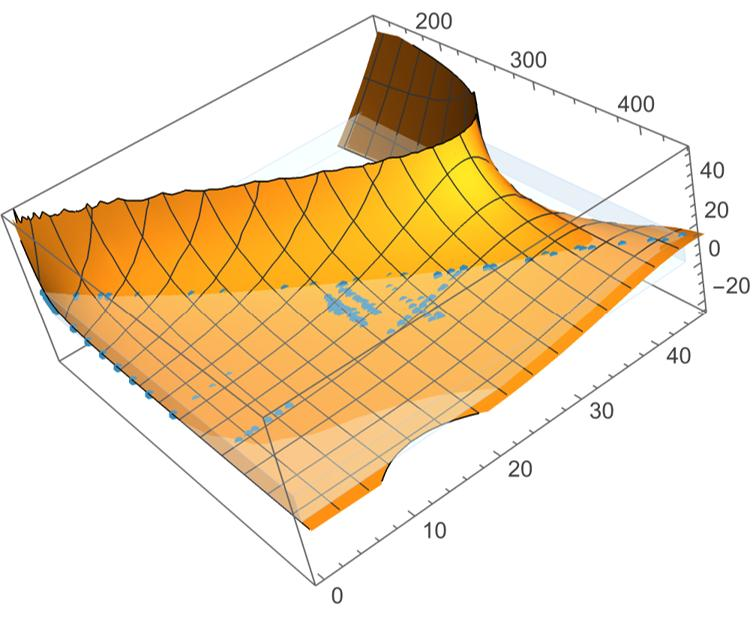
\includegraphics[width=0.9\textwidth]{SurfaceNonPhysicalPlot.jpg}
	
	\caption{Visualization of the non\textendash physical behavior inherent to the polynomial VTF surface expansion. At sufficiently high pressures the fitted surface fails to asymptotically approach zero mobility with decreasing temperature, instead exhibiting an nonphysical downturn in the predicted $\alpha$-relaxation time. This illustrates the limitations of the polynomial form used in \eqn\ref{eqn:VTFsurface}.}
	\label{figure:SurfaceNonPhysical}
\end{figure}


Even were this not the case, and it may not be for all liquids, the underlying issue remains\textemdash a polynomial expansion for the zero-mobility temperature and fragility functions, $T_{0}(P)$ and $D(P)$, is inherently non-physical. A model that better constrains the surface behavior, in particular its tendency to asymptotically approach a regime in which relaxation modes are suppressed (both for decreasing temperatures and increasing pressures), would be preferable to this simple polynomial expansion. For this reason, attention was turned toward creating a pressure–temperature dependent model of the $\alpha$-relaxation for which, regardless of the best-fit parameters, the physical requirement of an asymptotic approach to regions of zero mobility is maintained along any isobar or isotherm. For anyone familiar with developments in the glassy-dynamics community over the last few decades, the ``modified'' VTF (\eqn \ref{eqn:ModifiedVTFPressureClassic}) first suggested by Paluch \etal should come to mind\textemdash a natural analogue of the classic VTF but expressed as a function of pressure rather than temperature\cite{Paluch_1998}.
 

\begin{equation}
	\ln \langle \tau(P) \rangle
	= \ln \tau_{\infty}
	+ \frac{D_{P}\,P_{0}}{P_{0} - P},
	\label{eqn:ModifiedVTFPressureClassic}
\end{equation}

Historically, the modified VTF was introduced as a direct analogue of the classic VTF relation but reformulated for the pressure path. Paluch and co-workers demonstrated that, along an isotherm, the dramatic slowing down of molecular mobility with increasing pressure follows a divergence form that mirrors the temperature-driven Vogel--Tammann--Fulcher behavior. In this formulation, $P_{0}$ plays the role of a zero-mobility pressure, and $D_{P}$ quantifies the steepness of the divergence, thereby providing a pressure-based analogue of fragility. Because the modified VTF guarantees an asymptotic divergence of the relaxation time as $P \rightarrow P_{0}$, it naturally enforces physically reasonable behavior along every isotherm, in sharp contrast to the polynomial expansions used in \eqn\ref{eqn:VTFsurface}. This makes it particularly attractive for systems in which pressure-induced vitrification or dynamic arrest is expected, or for cases where extrapolation beyond the directly measured pressure range is required.

\subsection{Andersson--Andersson-constrained zero-mobility surface}

In \eqn \ref{eqn:VTFsurface} we introduced a Vogel--Tammann--Fulcher
(VTF) surface whose temperature--pressure curvature was constrained by
the Andersson--Andersson isochrone model fit to our \tgp data from \app \ref{app:CumeneIGP} near the glass-transition at approximately $\tau\approx 130\si{\second}$.
There, the AA model was used to enforce the physically required shape
of the boundary $T_{g}(P)$, while the VTF divergence retained its
usual temperature dependence.

Here we apply the same Andersson--Andersson model, but with a different
interpretation. Instead of modeling the glass-transition isochrone, we
assume that the \emph{zero-mobility} isochrone, the locus along which
the relaxation time diverges, shares the same AA-type curvature as
$T_{g}(P)$. The rationale is that both the glass transition and the
zero-mobility boundary reflect the same limiting physics of suppressed
structural relaxation at low temperature and high pressure.

\subsubsection*{Andersson--Andersson form for the zero-mobility isochrone}

The original AA expression for the glass-transition isochrone is as follows:
\begin{equation}
	T_{g}(P)
	= k_{1}\,\left(1 + \frac{k_{2}}{k_{3}}\,P\right)^{1/k_{2}}
	\label{eqn:AA_original}
\end{equation}
To repurpose this shape for the zero-mobility surface, we replace
$k_{1}$ by the zero-mobility temperature, or the temperature for which $\tau$ diverges to infinity, for the VTF model at 1-bar\textemdash $t_0$ from \eqn \ref{eqn:VTFsurface}.
\begin{equation}
	T_{0}(P)
	= T_{\infty}
	\left(1 + \frac{k_{2}}{k_{3}}\,P\right)^{1/k_{2}}
	\label{eqn:T0_of_P}
\end{equation}
Here $T_{\infty}=115.2\si{\kelvin}$ .  This  ensures that the zero mobility temperature provided by our AA constraint is in agreement with the 1-bar constraint from \fig  \ref{fig:cumene_VTF_1bar} as with our previous model.

The zero-mobility isochrone can equally well be expressed in terms of
the pressure required to reach divergence at a fixed temperature.  
To obtain this form, we simply solve the Andersson--Andersson expression
for $P$ rather than for $T$. 

\begin{equation}
	P_{0}(T)
	= \frac{k_{3}}{k_{2}}
	\left[\left(\frac{T}{T_{\infty}}\right)^{k_{2}} - 1\right]
	\label{eqn:P0_of_T}
\end{equation}


\subsubsection*{The AA-constrained two-variable VTF surface}

Constraining the zero-mobility isochrone introduces only two fit
parameters when used in conjunction with the 1-bar VTF constraint. It
is suggested here that a sufficient model for the relaxation dynamics of
a simple van-der-Waals liquid such as cumene, taking the form of
\eqn \ref{eqn:H_general}, requires only one additional degree of freedom\textemdash a
constant $D_{p}$ analogous to the fragility parameter $D_{0}$ in the
classical VTF expression.

\begin{equation}
	H(T,P) = \log(\tau_{\inf})
	+ \frac{D_{0}\,T_{0}(P)}{T - T_{0}(P)}
	+ \frac{D_p\,P}{P_{0}(T) - P}
	\label{eqn:H_general}
\end{equation}
Substituting \eqn \ref{eqn:T0_of_P} and \nolinebreak \eqn \ref{eqn:P0_of_T} into
\eqn\ref{eqn:H_general} gives the explicit form of \eqn \ref{eqn:H_final},
\begin{equation}
	H(T,P)
	= \log(\tau_{\inf})
	+ \frac{D_{0}\,T_{\infty}\left(1 + \frac{k_{2}}{k_{3}}\,P\right)^{1/k_{2}}}
	{T - T_{\infty}\left(1 + \frac{k_{2}}{k_{3}}\,P\right)^{1/k_{2}}}
	+ \frac{D_p\,P}
	{\displaystyle
		\frac{k_{3}}{k_{2}}
		\left[\left(\frac{T}{T_{\infty}}\right)^{k_{2}} - 1\right]
		- P },
	\label{eqn:H_final}
\end{equation}

\noindent
where $\tau_{\infty}=1.118179~\si{\pico\second}$, 
$T_{\infty}=115.201~\si{\kelvin}$, and $D_{0}=1.59655$ are fixed from the 1-bar constraint, leaving only $D_{p}$, $k_{2}$, and $k_{3}$ as degrees of freedom in the nonlinear surface fit.

The resulting parameter values are listed in \tbl  \ref{tab:Hgeneral_AA_surface_fits}.  
The corresponding fitted surface is shown in \fig \ref{fig:SurfaceZeroMobilityFit}, 
where the rear vertical isochrone surface represents the zero-mobility asymptote, 
and a second vertical isochrone surface marks the $130\,\si{\second}$ \tgp condition.  
The increasing separation between these two vertical isochrone surfaces with rising 
pressure reflects the expected decrease in fragility at higher pressures.

It is important to note that this model constitutes a zero-mobility–constrained 
surface. Both the \tgp and zero-mobility isochrones are generated using the same 
Andersson--Andersson regression; however, it is the additional modified-VTF-shaped 
constraint imposed along the isotherms that forces the relaxation dynamics to 
asymptotically approach a physically meaningful region of zero mobility for 
\emph{all} temperatures and pressures. 
This stands in sharp contrast to the earlier polynomial-expansion model, whose form 
allowed nonphysical behavior away from the data domain and did not enforce divergence 
along any thermodynamic path. 
By embedding the correct asymptotic structure directly into the surface, rather than 
attempting to approximate it with independent polynomial terms, the present model 
permits reliable extrapolation beyond the measured $(T,P)$ range. 
Such extrapolation is essential for assessing the pressure and temperature-dependent 
fragility, particularly in regions where direct measurements are not experimentally 
accessible.

\begin{figure}[!htbp]
	\centering
	\begin{tikzpicture}
		\node[anchor=south] at (0,0)
		{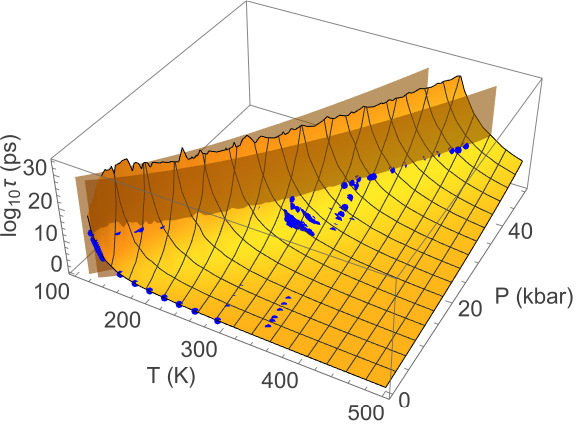
\includegraphics[width=0.92\linewidth]{Chapters/PCS/Figures/SurfaceZeroMobilityFit.png}};
		
		\node[anchor=south, yshift=2pt] at (0,12)
		{\large\bfseries Zero-Mobility Constrained Relaxation Surface};
	\end{tikzpicture}
	
	\caption[Relaxation-time surface constrained by the zero-mobility isochrone]{Fit surface resulting from the three-degree-of-freedom model of \eqn \ref{eqn:H_general}, constrained by the Andersson--Andersson representation of the zero-mobility isochrone. The rear vertical sheet represents this zero-mobility asymptote $T = T_{0}(P)$ (equivalently, $P = P_{0}(T)$), while the front vertical sheet follows the Andersson--Andersson fit to the TGP data provided in \app~\ref{app:CumeneIGP}. The curved surface shows the fitted relaxation landscape over $(T,P)$ space, with experimental data overlaid as blue points. The corresponding dataset, including percent errors defined as the deviation in $\log_{10}(\tau)$ from the fitted surface, is provided in \app~\ref{app:DPCSdata}.}
	\label{fig:SurfaceZeroMobilityFit}

\end{figure}


\begin{table}[!htbp]
	\centering
	
	\tabletitle{Fit parameters for the AA-constrained VTF surface model}
	\label{tab:Hgeneral_AA_surface_fits}
	
	\begin{tabular}{lccc}
		\toprule
		\textbf{Parameter} & \textbf{Estimate} & \textbf{Standard Error} & \textbf{t-Statistic / P-Value} \\
		\midrule
		$D_{p}$ 
		& 3.91293 
		& 0.228946 
		& $17.0911 \;/\; 3.60118\times 10^{-34}$ \\
		$k_{2}$ 
		& 1.71628 
		& 0.0125992 
		& $136.222 \;/\; 3.76332\times 10^{-135}$ \\
		$k_{3}$ 
		& 13.7721 
		& 0.213287 
		& $64.5708 \;/\; 3.49584\times 10^{-96}$ \\
		\bottomrule
	\end{tabular}
	
	\tabledescription{Fit parameters for the three-degree-of-freedom relaxation-surface model of \eqn\ref{eqn:H_general}. The table lists the parameter estimates together with their standard errors, $t$-statistics, and associated $p$-values derived from the nonlinear regression. These parameters define the Andersson--Andersson–constrained VTF surface for the zero-mobility isochrone.}
\end{table}

\begin{figure}[!htbp]
	\centering
	\begin{tikzpicture}
		\begin{axis}[
			width=0.85\linewidth,
			height=0.60\linewidth,
			xmin=0, xmax=4.7,
			ymin=120, ymax=460,
			xlabel={$P$ (\si{\giga\pascal})},
			ylabel={$T$ (\si{\kelvin})},
			grid=both,
			legend pos=north west,
			legend cell align=left,
			ticklabel style={/pgf/number format/fixed},
			]
			
			% Tg(P) data: col 2 = P (kbar), col 3 = T (K)
			\addplot[
			only marks,
			mark=*,
			mark size=2.2pt,
			mark options={blue}
			] table[
			col sep=space,
			x expr=\thisrowno{1}/10, % kbar -> GPa
			y index=2
			] {Chapters/PCS/Figures/TGPIsocroneData.txt};
			
			% Andersson--Andersson fit to Tg(P)
			\addplot[
			thick,
			dashed,
			domain=0:4.7,
			samples=200
			] {131.145*(1 + (1.64181/12.1852)*x*10)^(1/1.64181)};
			
			% Zero-mobility AA isochrone
			\addplot[
			very thick,
			red,
			domain=0:4.7,
			samples=200
			] {115.201*(1 + (1.68164/14.2038)*x*10)^(1/1.68164)};
			
			\legend{
				$T_{\mathrm{g}}(P)$ data,
				AA fit to $T_{\mathrm{g}}(P)$,
				zero-mobility AA isochrone
			}
			
		\end{axis}
	\end{tikzpicture}
	\caption[Cumene $T_{\mathrm{g}}(P)$ and AA isochrones]{
		Cumene glass-transition temperatures $T_{\mathrm{g}}(P)$ with the Andersson--Andersson fit from \app\ref{app:CumeneIGP}, together with the AA zero-mobility isochrone for comparison  (red line) shown as the rear vertical sheet in \fig \ref{fig:SurfaceZeroMobilityFit}.  The decrease in the classical isobaric fragility with increasing pressure is evident in the growing separation between these two isochronal curves.
		
	}
	\label{fig:CumeneIGP_AA_ZeroMobility}
\end{figure}

It is evident from inspection of the relaxation surface in \fig  \ref{fig:SurfaceZeroMobilityFit} that the fragility of cumene decreases with increasing pressure.  In the present framework, fragility is
defined not through the classical VTF parameters of the earlier polynomial model, but directly from
the geometry of the logarithmic relaxation surface
\begin{equation}
	H(T,P)\equiv \log_{10}\tau_{\alpha}(T,P),
\end{equation}
given by the Andersson–Andersson–constrained VTF form of \eqn \ref{eqn:VTFsurface}.
This formulation naturally allows fragility to be expressed in terms of the gradient of the surface,
thereby providing a more physical interpretation of how relaxation modes are suppressed along
isobars and isotherms.

\subsubsection*{Temperature–based scaled  fragility}
Following the scaled definition of fragility introduced in \sect\ref{sec:Fragility} (\eqn\ref{eqn:scaledfragility}), the isobaric scaled fragility is obtained by differentiating $H(T,P)$ with respect to the reduced temperature $T_{g}(P)/T$ at fixed pressure:
\begin{equation}
	m^{*}(P)
	\equiv
	\left.
	\frac{1}{\Delta}
	\frac{\partial H}{\partial\!\left( T_{g}(P)/T \right)}
	\right|_{T=T_{g}(P)}
\end{equation}
where $\Delta=\log_{10}(\tau_{g}/\tau_{\infty})$ is the scaled dynamic range between the
infinite–temperature and glass–transition relaxation times.  Because $T_{g}(P)$ is constant along an
isobar,
\[
\frac{\partial}{\partial (T_{g}/T)} = -\frac{T^{2}}{T_{g}}\,\frac{\partial}{\partial T}
\]
and therefore the scaled  fragility can be written compactly in terms of the gradient of the relaxation
surface:
\begin{equation}
	\label{eqn:mpstar_surface}
	m^{*}(P)
	=
	-\frac{T_{g}(P)}{\Delta}
	\left.
	\left( \nabla H \right)_T
	\right|_{T=T_{g}(P)}
\end{equation}

Physically, this quantity reflects how rapidly the dynamics slow when the temperature is decreased
slightly below $T_{g}(P)$ at fixed pressure.  Because small variations in temperature do not strongly
modify the underlying potential–energy landscape near the glass transition, $m^{*}(P)$ primarily
characterizes the \emph{probe response} of the system—how sharply the available relaxation pathways
become dynamically inaccessible as thermal energy is withdrawn. A strong argument was made previously for the adoption of the scaled fragility definition given in \eqn \ref{eqn:scaledfragility}. Nevertheless, to facilitate direct comparison between fragility values derived from the present surface and those reported elsewhere in the literature, it is appropriate to continue working with the classical Angell definition of fragility. Accordingly, results will primarily be discussed in terms of the conventional fragility, although, where easily accommodated, both definitions will be presented.

Before proceeding to an analysis of the pressure dependence of isobaric fragility, it is first necessary to address the fragility of cumene at atmospheric pressure. Reported values of this parameter exhibit a notable degree of variability within the literature, even after accounting for differences in how the glass transition temperature is defined, with most studies adopting the standard criterion of $\tau = 100\,\si{\second}$. Understanding the origin of this discrepancy serves not only to validate the surface model developed here, which relies critically on a fixed isobaric regression at atmospheric pressure, but also to reinforce a conclusion that is already well established in the literature. Specifically, light scattering experiments, as a non-invasive probe, provide a more faithful measure of the intrinsic $\alpha$-relaxation associated with the stochastic thermal evolution of the system, even in a comparatively simple liquid such as cumene, which might otherwise be expected to lend itself equally well to dielectric spectroscopy and DPCS.

Our surface model, anchored by a 1--bar VTF regression, relies on data collected by Hansen \etal \cite{Hansen2018} and Li \etal \cite{Li1995CumenePRL}, together with the \tgp point derived from the Andersson--Andersson fit described in \app\ref{app:CumeneIGP}. \fig  \ref{fig:cumene_VTF_1bar} demonstrates remarkably good agreement between the model and the data over the full dynamic range. A slight tendency for the VTF fit to underestimate the data is observed as temperatures approach $160\,^{\circ}\mathrm{C}$; however, this region lies near the upper operational limit of Brillouin light scattering, where the extracted relaxation times begin to approach the Bose peak. Consequently, confidence in these intermediate--temperature points is reduced.

Importantly, a substantial body of ambient--pressure data exists for cumene, and the 1--bar datasets employed here were selected specifically because they were obtained using light--scattering probes\textemdash DPCS in the case of Hansen \etal and Brillouin light scattering in the work of Li \etal The \tgp point would likewise be expected to provide a direct measure of the structural relaxation, as few experimental observations are more direct than the physical vitrification of the material. However, as discussed previously in the description of the surface model, the precise relaxation time $\tau_i$ associated with this isochrone is not directly experimentally measurable and is instead constrained by where it crosses this atmospheric VTF isobar. The corresponding isochronal value is nonetheless independently verifiable in the case of cumene via the intercept obtained from the thermodynamic scaling of the data shown in \fig \ref{figure:tdscaling}.

\iffalse
The strong adherence of our data to a VTF description, shown in \fig \ref{fig:cumene_VTF_1bar}, may be contrasted with the behavior inferred from dielectric spectroscopy in the work of Chen and Richert~\cite{Chen}. That study had a different focus and did not report new measurements of the relaxation dynamics of cumene (iso-propylbenzene), but instead compiled bulk dielectric and viscosity data from three prior sources. These compiled data were used to extract a classical Angell fragility for cumene of $m=77.6$, a comparatively high value relative to others reported in the literature.

It is important to emphasize, however, that this fragility does not arise from the slope of a single global VTF fit applied over the full temperature range of the compiled dataset. As shown in \fig \ref{fig:Chen_global_VTF}, a global VTF regression significantly overestimates the relaxation times in the intermediate-temperature regime while underestimating the data in the region of faster dynamics. This stands in marked contrast to the fidelity demonstrated by the VTF fit to the Hansen \etal and Li \etal light-scattering data in \fig \ref{fig:cumene_VTF_1bar}. Such behavior is not unexpected: the low-viscosity regime lies within the optimal sensitivity range for Brillouin light-scattering measurements, while simultaneously approaching the practical limits of dielectric spectroscopy due to both instrumental bandwidth constraints and possible overlap with secondary fast relaxation processes.

Although a fragility may be formally extracted from the global VTF fit, yielding a notably high value of $m=91$, fragility is fundamentally defined by the slope of the relaxation dynamics at the glass transition, rendering curvature far from this transition of limited relevance. Accordingly, Chen and Richert adopted the more robust approach of fitting the VTF equation exclusively to data within the viscous regime approaching $T_g$. This restricted fitting window, together with the corresponding ``viscous'' VTF regression, is indicated by the shaded region in \fig \ref{fig:Chen_global_VTF}. When fragility is determined solely from data within this regime, a more moderate value of $m=74$ is obtained, in closer alignment with physical expectations.

\definecolor{cumeneMagenta}{RGB}{170,60,170}
\begin{figure}
	\centering
	\begin{tikzpicture}
		\begin{axis}[
			width=0.80\linewidth,
			height=0.60\linewidth,
			xmin=120,
			xmax=350,
			ymin=0,
			ymax=16,
			xlabel={$T$ (K)},
			ylabel={$\log_{10}\tau_{\alpha}$ (s)},
			legend pos=north east,
			legend cell align=left,
			grid=both,
			ticklabel style={/pgf/number format/fixed},
			]
			
			%------------------------------------------------------------
			% Data set 1: open purple triangles
			%------------------------------------------------------------
			\addplot[
			only marks,
			mark=triangle,
			color=purple,
			mark options={draw=cumeneMagenta, fill=none},
			]
			table[
			x=triangleX,
			y=triangleY,
			col sep=comma,
			]{ChenVTF.csv};
			\addlegendentry{Barlow \cite{Barlow}}
			
			%------------------------------------------------------------
			% Data set 2: open purple circles
			%------------------------------------------------------------
			\addplot[
			only marks,
			color=purple,
			mark options={draw=cumeneMagenta, fill=none},
			]
			table[
			x=openX,
			y=openY,
			col sep=comma,
			]{ChenVTF.csv};
			\addlegendentry{Gangasharan \cite{Gangasharan}}
			
			%------------------------------------------------------------
			% Data set 3: closed purple circles
			%------------------------------------------------------------
			\addplot[
			only marks,
			mark=*,
			color=purple,
			mark options={draw=cumeneMagenta, fill=purple},
			]
			table[
			x=closedX,
			y=closedY,
			col sep=comma,
			]{ChenVTF.csv};
			\addlegendentry{Nielsen \cite{Nielsen}}
			
			%------------------------------------------------------------
			% Global VTF regression fit (your fitted parameters):
			% y = a + B/(T - c)
			% B = 305.881, a = -.724953, c = 107.395
			%------------------------------------------------------------
			\addplot[
			red,
			thick,
			domain=120:350,
			samples=200,
			]
			{ -.724953 + 305.881/(x - 107.395) };
			\addlegendentry{VTF (global)}
			
			%------------------------------------------------------------
			% Vicous VTF regression fit (your fitted parameters):
			% y = a + B/(T - c)
			% B = 600.143, a = -4.62659, c = 95.5547
			%------------------------------------------------------------
			\addplot[
			blue,
			thick,
			dashed,
			domain=120:350,
			samples=200,
			]
			{ -4.62659 + 600.143/(x - 95.5547) };
			\addlegendentry{VTF (viscous)}
			
			%------------------------------------------------------------
			% Equation box (kept identical to your style)
			%------------------------------------------------------------
			\node[
			anchor=north east,
			fill=white,
			draw=black,
			rounded corners=2pt,
			inner sep=4pt
			]
			at (rel axis cs:.98,0.65)
			{%
				$\displaystyle
				\ln\tau = \ln\tau_{\infty}
				+ \frac{D T_{0}}{T - T_{0}}$
			};
			
			%------------------------------------------------------------
			% Shaded region indicating viscous-fit temperature window
			%------------------------------------------------------------
			\addplot [
			draw=none,
			fill=gray,
			fill opacity=0.15,
			]
			coordinates {
				(120,0)
				(155,0)
				(155,16)
				(120,16)
				(120,0)
			};
			
			
		\end{axis}
	\end{tikzpicture}
	
	\caption{Atmospheric-pressure relaxation data for cumene compiled by Chen and Richert, plotted as $\log_{10}\tau_{\alpha}$ versus temperature\cite{Chen}. With the exception of the data of Barlow \cite{Barlow}, which consist of viscosity measurements converted to relaxation times via the Maxwell relation using a constant high-frequency shear modulus $G_{\infty}=0.04\,\text{GPa}$, all data shown were obtained via dielectric spectroscopy. The solid red curve represents a single VTF regression applied over the full temperature range of the compiled dataset.  However, this global fit does not adequately capture the behavior of the data in the low-viscosity (high-temperature) regime. The fragility value of $m=77.6$ reported by Chen and Richert was therefore obtained from a VTF fit restricted to the viscous regime near the glass transition, indicated by the shaded region, with the corresponding VTF regression shown by the dashed blue curve.}
	
	\label{fig:Chen_global_VTF}
\end{figure}

The slightly higher value of $m=77.6$ reported by Chen and Richert reflects their particular selection of data within this viscous regime. While the specific rationale for excluding a substantial fraction of the available viscous-domain data is not explicitly discussed, such a choice may reasonably be motivated by an effort to avoid disproportionate weighting of data clustered near the glass transition or to maintain a more uniform spacing of points in the fitting procedure. Regardless of the motivation, this selective treatment introduces a nontrivial variation in the extracted fragility, underscoring the sensitivity of fragility to both the chosen fitting window and the details of the fitting methodology.

The purpose of the preceding discussion has been to clarify the rationale behind our choice to anchor the atmospheric-pressure VTF isobar of the surface model using light-scattering data, despite the more limited availability of such measurements within the literature, as well as to make the argument for why light scattering is, even in the case of cumene, and arguably superior probe of structural relaxation dynamics. While it is well established that differing values of fragility may be obtained depending on the experimental probe, or even minor differences in data analysis, fragility itself is not a sharply defined material constant in the same sense as, for example, the speed of sound or the location of a first-order phase transition. Rather, it is derived from the behavior of a second-order glass transition and is therefore inherently more sensitive to both experimental methodology and data treatment. Nevertheless, fragility remains a quantity of significant physical interest, and if  confidence is to be placed in values extracted from a surface construction, it is essential that the limiting cases such as the atmospheric-pressure constraint be as reliable as possible.

Cumene, by virtue of its molecular simplicity and predominantly van der Waals interactions, might reasonably be expected to be equally amenable to characterization by dielectric spectroscopy and light-scattering techniques. There is, however, no fundamental guarantee that a phenomenological form such as the VTF equation should accurately describe structural-relaxation data spanning fourteen decades in time. Even so, the light-scattering measurements of Hansen \etal and Li \etal are more uniformly and robustly described by VTF regression over their experimentally accessible dynamic range than are corresponding dielectric-based compilations. Given both the indirect nature of dielectric spectroscopy and its practical limitations as the dynamics approach the high-frequency regime, it is therefore reasonable to construct the atmospheric-pressure constraint of the surface model using light-scattering data. Doing so increases confidence not only in the extracted atmospheric fragility but also in the associated $\alpha$-relaxation times and derived quantities that depend on this limiting behavior. More generally, dielectric spectroscopy and depolarized photon-correlation spectroscopy probe distinct relaxation channels, and parameters such as fragility are intrinsically sensitive to how these channels are weighted. Consequently, while dielectric spectroscopy remains an essential and broadly applicable technique, light-scattering methods, where experimentally accessible, provide a more direct and reliable measure of collective glassy dynamics.


\fi
\subsubsection*{Pressure dependence of fragility}
The surface model defined in \eqn \ref{eqn:H_final} provides a robust and internally consistent framework for examining the pressure dependence of isobaric fragility. In the discussion that follows, we focus primarily on the conventional Angell fragility in order to facilitate direct comparison with previously reported literature values. For completeness, the pressure dependence of both the conventional fragility and the scaled fragility $m^{*}(P)$ defined in \eqn \ref{eqn:mpstar_surface} are shown in \fig  \ref{figure:fragilityPressure}. 

At ambient pressure, the fragility extracted from the present surface lies slightly below commonly cited values for cumene. Dielectric analyses typically report fragilities in the range $m \approx 70$--$80$, for example $m = 77.6$ as obtained by Chen and Richert \cite{Chen}, and values near $m \approx 70$--$75$ as compiled by Wang \etal \cite{Wang}. In contrast, light-scattering-based determinations, such as those derived from Brillouin and photon-correlation measurements of cumene \cite{Li1995CumenePRL}, tend to yield somewhat lower values. This difference is likely also partially attributable to the manner in which fragility is evaluated within the present framework. Specifically, the fragility reported here is obtained directly from the local gradient of the relaxation-time surface, rather than from fits restricted exclusively to the viscous regime. As a consequence, the resulting value is sensitive to the overall goodness of fit across the accessible dynamic range, rather than being dominated by enforced low-temperature curvature alone.

\begin{figure}[!htbp]
	\centering
	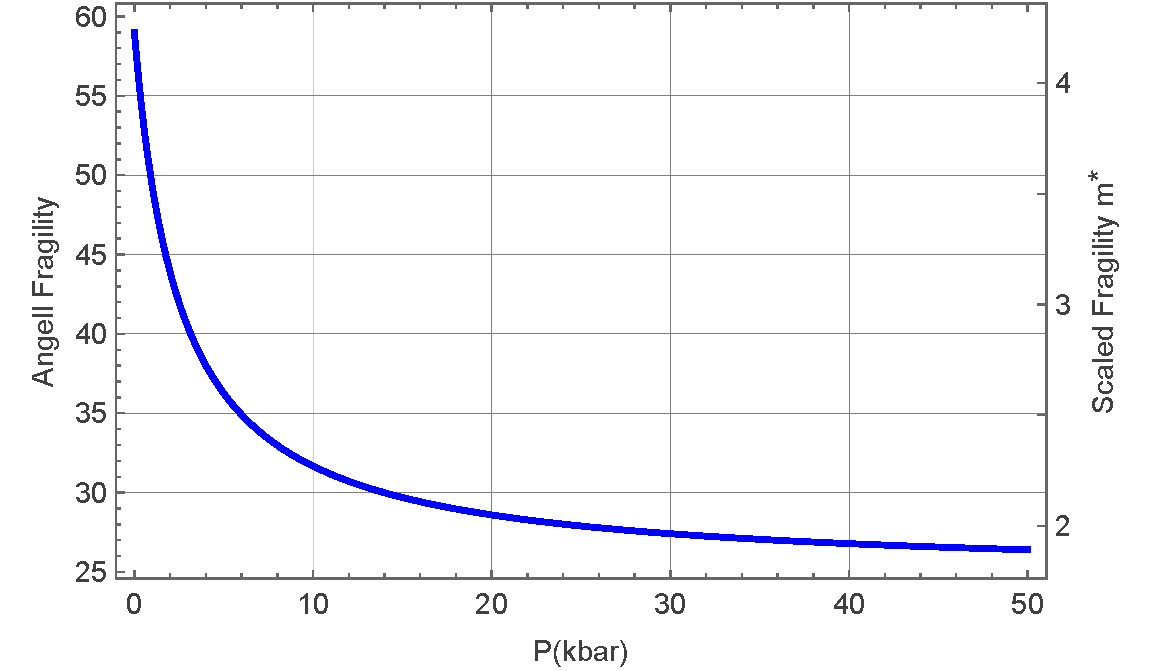
\includegraphics[width=0.9\linewidth]{PressureVsFragility.pdf}
	\caption{
		Pressure dependence of the isobaric fragility of cumene obtained from the relaxation-time surface. The left axis shows the conventional Angell fragility $m$, while the right axis displays the scaled fragility $m^{*}$ defined in \eqn \ref{eqn:mpstar_surface}. When viewed in terms of the scaled fragility, the data clearly suggest an asymptotic approach toward a finite high-pressure limit that retains more fragility than would arise from purely Arrhenius behavior.
	}
	\label{figure:fragilityPressure}
\end{figure}


Despite this modest reduction in magnitude at low pressure, the qualitative pressure evolution of the fragility is clear and robust. The fragility exhibits a smooth but distinctly nonlinear decline with increasing pressure, consistent with the growing separation between the glass-transition isochrone $T_g(P)$ and the zero-mobility isochrones shown in \fig  \ref{figure:SurfaceFit}. With increasing pressure, the system becomes progressively stronger, approaching Arrhenius-like behavior, consistent with a stiffening of the underlying relaxation landscape.

One particularly striking feature of this model is the emergence of a high-pressure asymptote as demonstrated in \sect \ref{sec:asymptote}. It is often implicitly assumed that increasing pressure yields a stronger liquid, with the limiting case being purely Arrhenius behavior. Although the fragility of cumene decreases rapidly as cooperative dynamics are suppressed, these dynamics do not appear to be fully eliminated. The limiting fragility obtained from the surface model of \eqn \ref{eqn:H_final} as pressure approaches infinity is approximately $m^* = 1.8$, corresponding to $m = 25$ in terms of the conventional Angell fragility. This represents a clear instance in which the utility of the scaled fragility defined in \eqn \ref{eqn:scaledfragility} becomes evident. As shown in \fig  \ref{figure:fragilityPressure}, even without extrapolation beyond the experimentally accessible data, the scaled fragility is clearly converging toward a value significantly greater than unity. This limiting behavior remains distinctly more fragile than that of a purely Arrhenius system, indicating that increasing pressure does not drive the liquid into a truly strong glass-forming regime. Instead, the surface model suggests the persistence of residual non-Arrhenius character even at very elevated pressures, consistent with an energy landscape that becomes increasingly stiff while retaining a finite degree of dynamical heterogeneity.

The existence of this asymptotic fragility is not imposed by the model but rather it emerges naturally from the global structure of the relaxation-time surface. The rapid approach toward this asymptote well within the domain of the available relaxation data lends confidence to its physical significance. At least in the case of cumene, it appears that the system cannot be driven fully into Arrhenicity by the application of pressure alone.


\subsubsection*{Isothermal pressure–modified fragility}

An entirely analogous expression follows for compression along isotherms. Defining the glass--transition pressure $P_{g}(T)$ via $H\!\left(T,P_{g}(T)\right)=\log_{10}\tau_{g}$, the pressure--modified fragility is defined with respect to the reduced pressure and may be written as
\begin{equation}
	m^{*}_{P}(T)
	\equiv
	\left.
	\frac{1}{\Delta}
	\frac{\partial H}{\partial (P/P_{g}(T))}
	\right|_{P=P_{g}(T)}
	=
	\frac{P_{g}(T)}{\Delta}
	\left.
	(\nabla H)_P
	\right|_{P=P_{g}(T)}
\end{equation}


In contrast to temperature variation, increasing pressure directly alters the intermolecular structure: local cages tighten, barrier heights increase, and the potential–energy landscape itself is reshaped. Thus $m^{*}_{P}(T)$ represents a \emph{susceptibility of the landscape to mechanical compression}, rather than a probe of dynamical accessibility.

For this reason, it is the opinion of the author that the isothermal pressure--modified fragility should be understood as fundamentally \emph{not} a measure of landscape fragility; rather, it quantifies how readily the landscape itself deforms under pressure—no more a ``fragility'' than EMF is a force. Even so, it remains a useful parameter when investigating vitrification under compression, particularly as one approaches pressures for which all relaxation modes are suppressed and the structural entropy becomes effectively locked in. This ``pressure quenching'' is, in many cases, a more practical route to rapid vitrification when thermal quenching is too slow to avoid crystallization.

\subsubsection*{Connection to activation volume}

The same isothermal pressure derivative that defines the pressure--modified fragility also
appears naturally in the conventional definition of the activation volume.
For a relaxation process described by
$\tau(T,P)$, the molar activation volume is defined as
\begin{equation}
	\label{eqn:activationVolume}
	\Delta V^{\ddagger}(T,P)
	\equiv
	RT
	\left.
	\frac{\partial \ln \tau(T,P)}{\partial P}
	\right|_{T},
\end{equation}
where $R$ is the universal gas constant.
Expressed in terms of the surface 
$H=\log_{10}\tau$ implemented here, \eqn\ref{eqn:activationVolume} becomes

\begin{equation}
	\Delta V^{\ddagger}(T,P)
	=
	(\ln 10)\,RT
	\left.
	(\nabla H)_P
	\right|_{T}.
\end{equation}

Evaluated along the glass--transition isochrone $P=P_{g}(T)$, the activation volume is therefore
directly proportional to the same local surface derivative that enters the definition of the
pressure--modified fragility:
\begin{equation}
	\Delta V^{\ddagger}_{g}\!\left(T,P_{g}(T)\right)
	=
	(\ln 10)\,R\,T\,
	\frac{\Delta}{P_{g}(T)}\,
	m^{*}_{P}(T).
	\label{eqn:mpstar_activationVolume}
\end{equation}

This relation makes explicit that $m^{*}_{P}(T)$ provides a scaled measure of the pressure sensitivity of the dynamics, normalized by the glass--transition pressure and the accessible dynamic range. When combined with the appropriate thermodynamic prefactors, it yields the conventional activation volume $\Delta V^{\ddagger}_{g}(T,P)$, which retains its usual interpretation as a molar volume characterizing pressure--induced slowing of the structural dynamics.

Within the surface--based framework developed here, activation volume and modified fragility are
thus revealed to be complementary projections of the same relaxation--surface gradient.
The distinction lies not in the derivative itself, but in the physical interpretation imposed by the
choice of scaling: multiplication by $P_{g}(T)$ yields a scaled susceptibility describing how
readily the relaxation landscape deforms under compression, whereas multiplication by $RT$
recovers the conventional activation volume familiar from high--pressure relaxation studies.
This unification clarifies the relationship between pressure fragility and activation volume without
requiring separate fits or auxiliary models, and highlights the utility of the constrained surface in
providing physically consistent derivatives across the full $(T,P)$ domain.

\subsubsection*{Isochronic fragility and surface geometry}

The preceding measures of fragility emphasize either thermal variation at fixed pressure or mechanical compression at fixed temperature. A more neutral characterization follows by considering variations taken \emph{along an isochrone} of the relaxation surface itself. Within the present framework, this quantity arises naturally from the local geometry of the surface $H(T,P)$ and requires no additional fitting assumptions.

Along an isochrone defined by $H(T,P)=\log_{10}\tau=\mathrm{const}$, the total differential vanishes,
\begin{equation}
	\left.
	\frac{\partial H}{\partial T}
	\right|_{P} dT
	+
	\left.
	\frac{\partial H}{\partial P}
	\right|_{T} dP
	=0,
\end{equation}
so that the slope of the isochrone in the $(T,P)$ plane is given by
\begin{equation}
	\label{eqn:isochronicSlope}
	\left.
	\frac{dP}{dT}
	\right|_{H}
	=
	-
	\frac{
		\left(\partial H/\partial T\right)_{P}
	}{
		\left(\partial H/\partial P\right)_{T}
	}.
\end{equation}

This ratio of surface–gradient components provides a direct measure of the relative influence of temperature and pressure on the dynamics at fixed relaxation time and may be identified as an isochronic fragility. Unlike isobaric or isothermal measures, this quantity does not privilege a particular thermodynamic path, but instead reflects the intrinsic geometry of the relaxation surface.

If an equation of state is invoked to transform the surface from $(T,P)$ to $(T,V)$ coordinates, an equivalent isochronic fragility may be obtained in terms of the slope of constant--$\tau$ contours in $(T,V)$ space. In this representation, the separation between thermal and volumetric contributions to the dynamics becomes explicit, and the conventional isochoric fragility discussed in the literature is recovered as a particular projection of the same surface geometry. The agreement between these equivalent constructions emphasizes that isochronic, isobaric, and isochoric fragilities are not independent material properties, but rather complementary manifestations of the same underlying relaxation landscape.
  %Temporarily changed to working folder while changes are made


%\include{Chapters/Result2/Res2}
%\include{Chapters/Instrumentation/instrument} //This was added to apppendix
\chapter{Conclusion}

This dissertation has advanced the study of structural relaxation in glass-forming liquids by combining new experimental capability with a physically grounded framework for interpreting dynamics in thermodynamic space. The central result is a shift from describing relaxation along isolated thermodynamic paths to treating it as a continuous surface, $\tau(P,T)$, constrained by both experiment and physical boundary conditions.

On the experimental side, depolarized photon correlation spectroscopy (DPCS) was successfully extended into a diamond anvil cell environment, enabling direct measurement of structural $\alpha$-relaxation times at pressures approaching 2.5~GPa. This represents a significant expansion of the accessible thermodynamic space for optical probes of glassy dynamics, overcoming challenges associated with reduced scattering volume, heterodyne contamination, and photon-limited statistics. These measurements establish that DPCS remains a viable and powerful probe of structural relaxation under extreme conditions.

On the modeling side, relaxation dynamics were recast as a pressure--temperature surface, allowing fragility to be interpreted geometrically rather than as a purely isobaric quantity. By anchoring this surface to experimentally determined isochrones and incorporating physically motivated constraints, including a zero-mobility limit, the resulting framework avoids arbitrary extrapolation and provides a consistent description across broad thermodynamic ranges. Integration of high-pressure DPCS data with complementary dielectric and Brillouin measurements yields a unified representation of relaxation behavior.

Taken together, these results demonstrate that structural relaxation is inherently multi-dimensional, and that meaningful interpretation requires investigation across both temperature and pressure dimensions. The development of a thermodynamic surface model allows for the study of fragility as a function of both parameters and provides a pathway toward a more complete understanding of glass-forming systems.

Further refinement of the thermodynamic surface may be achieved through expansion of the TGP framework to multiple isochrones. By constraining the surface at several fixed relaxation times, rather than a single isochronal condition, the model can be more tightly anchored in the region surrounding the glass transition, where the most significant dynamical changes occur.

While Vogel--Tammann--Fulcher (VTF) behavior, and its modified forms along isothermal paths, appears to describe the dynamics of relatively simple liquids such as cumene with reasonable accuracy, it is well established that such models do not universally capture liquid dynamics across their full dynamic range. In contrast, our results indicate that the Andersson--Andersson formulation provides an exceptionally good description of the data along isochronal paths for both cumene and the hydrogen-bonded system glycerol---even through the transition associated with hydrogen-bond suppression. This observation raises the possibility that the Andersson--Andersson framework may serve not only as a high-pressure constraint, but as a more fundamental basis for constructing the full relaxation-time surface.

If such an approach proves broadly applicable, it invites deeper investigation into why this formulation succeeds under isochronal conditions. One possible interpretation is that isochronal paths, closely related to isochoric trajectories, more directly reflect the underlying physics governing structural relaxation. Future work may focus on testing this hypothesis and determining whether isochronal representations provide a more natural framework for describing glass-forming dynamics.

%\bibliographystyle{ieeetr}
 \printbibliography
%BACK MATTER/APPENDICES


%back matter are the microEP appendices
 \graphicspath{{Chapters/back_matter/Figures/}}
\appendix

\chapter{\tgp Data (Glycerol)} \label{app:GlycerolIGP}

\sisetup{
	round-mode          = places,
	round-precision     = 3,
}

\begin{table}[h!]
	\centering
	\caption{Glycerol \tgp Data}
	\label{table:IGPdataGlycerol}
	\pgfplotstabletypeset[
	multicolumn names,
	col sep=comma,
	display columns/0/.style={
		column name=Pressure,
		column type={S},
		string type
	},
	display columns/1/.style={
		column name=Temperature,
		column type={S},
		string type
	},
	display columns/2/.style={
		column name=Volume,
		column type={S},
		string type
	},
	every head row/.style={
		before row={\toprule},
		after row={
			\si{\giga\pascal} & \si{\kelvin} & \si{\cubic\centi\meter\per\gram}\\
			\midrule
		}
	},
	every last row/.style={after row=\bottomrule},
	]{Chapters/Back_matter/Figures/GlycerolTGPdata.csv}
\end{table}

\vspace{-0.5em}
{\small
	\noindent $^{*}$ Specific volumes corresponding to this pressure and above were obtained with moderate  to significant extrapolation of the Tait EOS beyond Bridgman's data.
	\par}

\begin{equation}
	\label{equ:IGPglycerol}
	T_{G}(P)=188.376\left ( 1+2.046\frac{P}{5.596} \right )^{\frac{1}{2.046}}
\end{equation}

\chapter{\tgp Data (Cumene)} \label{app:CumeneIGP}

\sisetup{
	round-mode          = places, % Rounds numbers
	round-precision     = 3, % to 2 places
}

\begin{table}[h!]
	\begin{center}
		\caption{Cumene \tgp Data}
		\label{table:IGPdata}
		\pgfplotstabletypeset[
		multicolumn names, % allows to have multicolumn names
		col sep=comma, % the separator in our .csv file
		display columns/0/.style={
			column name=Pressure, % name of first column
			column type={S},string type},  % use siunitx for formatting
		display columns/1/.style={
			column name=Temperature,
			column type={S},string type},
		display columns/2/.style={
			column name=Volume,
			column type={S},string type},
		every head row/.style={
			before row={\toprule}, % have a rule at top
			after row={
				\si{\GPa} & \si{\kelvin} & \si{\cubic\centi\meter\per\gram}\\ % the units seperated by &
				\midrule} % rule under units
		},
		every last row/.style={after row=\bottomrule}, % rule at bottom
		]{Chapters/Back_matter/Figures/CumeneTGPdata.csv} % filename/path to file
	\end{center}
\end{table}

\begin{equation}
\label{equ:IGPcumene}
T_{G}(P)=131.145\left ( 1+1.64181\frac{P}{1.21852} \right )^{\frac{1}{1.64181}}
\end{equation}

%cumene IGP data

\chapter{Equation of State (glycerol)} \label{app:GlycerolEOS}
To facilitate the conversion of glycerol pressure data ($\si{\giga\pascal}$) to molecular volume $\nicefrac{\si{\angstrom\cubed}}{molecule}$ the Tait equation of state, fit to Bridgman's glycerol data \cite{BridgmanGly}, was implemented.  It should be noted that Bridgman only obtained PVT data up to just under $1.2\;\si{\giga\pascal}$ yet Cook \etal extrapolates this equation of state up to $3\;\si{\giga\pascal}$ \cite{Cook2}. This work extrapolates this equation of state up to $6.68\;\si{\giga\pascal}$ to allow for the thermodynamic scaling assessment of \sect \ref{sec:GlycerolScaling}.  Clearly, experimental measurement of the glycerol equation of state at these elevated pressures is desperately needed yet remains absent within the literature.  However, despite dependence upon these extreme extrapolations, thermodynamic scaling of glycerol data implementing this equation of state yields self-consistent results as was demonstrated in \fig \ref{figure:GlycerolIGPScaling}. The isothermal Tait equation of state is given as follows:

\begin{equation} 
\frac{V}{V_0}=1-c\times ln\left(\frac{b+P}{b+P_0}\right),
\label{eqn:tait}
\end{equation}

\noindent where $P_0$ and $V_0$ are simply arbitrarily chosen reference values of pressure and volume, respectively, at a specific temperature.  For this work $P_0$ was set to atmospheric pressure and $V_0$ was found to be sufficiently well modeled as a linear function of temperature as follows:
\begin{equation}
V_0(T)=0.065T + 119.7,
\label{eqn:vo}
\end{equation} 
where temperature, T, is expected in ($\si{\degreeCelsius}$) and the resulting specific volume, $V_0$, is returned in units of ($\nicefrac{\si{\angstrom\cubed}}{molecule}$).  The density data for glycerol to which \eqn \ref{eqn:vo} was fit was taken from Cheng \nolinebreak\cite{Cheng}. The remaining fit parameters $c$ and $b$ may be trivially related to the bulk modulus $K_0$ and its pressure derivative $K_{0}^{'}$ via \eqn \ref{eqn:abtait}.   
\begin{equation} 
K_0=\frac{P_0}{c}+\frac{b}{c}\:\:\:\:\:\:
and\:\:\:\:\:\:
K_{0}^{'}=\frac{1}{c}-1-Log\left ( \frac{b}{b+P_0} \right )
\label{eqn:abtait}
\end{equation} 
The reported values of the bulk modulus, $K_0$, and its pressure derivative, $K_{0}^{'}$, calculated from five separate isothermal Tait equations of state by Cook \etal was fit to a third order polynomial model shown in \fig \ref{figure:GlycerolBulkMod}.  This enables accurate interpolation of $K_0$ and $K_{0}^{'}$ at any arbitrary temperature within this range.
\begin{figure}[H]
\centering
\begin{tikzpicture} 
\begin{axis}[
title={Glycerol Bulk Modulus and Pressure Derivative},
ylabel={$\color{blue}\square$ Bulk Modulus, $K_0$ ($\si{\giga\pascal}$)},
xlabel={Temperature ($\si{\degreeCelsius}$)},
ymin=2.8, ymax=5,
xmin=0, xmax=130,
%xtick={0,.002,.004,.006,.008,.01},
ytick={3,3.5,4,4.5,5},
width=0.9\textwidth,
height=3in
]

	\addplot+[only marks, mark=square]
	coordinates { 
		(0,4.83)
		(22.5,4.34)
		(50,3.91)
		(75,3.61)
		(125,3.13)};
	
	\addplot expression[domain=0:130,mark=none,red]{
	-0.00000048585*x^3+0.00014985*x^2-.024734*x+4.8291};
	
\end{axis}

\begin{axis}[
xmin=0,xmax=130,
ymin=6.8,ymax=9,
ytick={7,7.5,8,8.5,9},
axis y line*=right,
axis x line=none,
ylabel style = {align=center},
ylabel={$\color{blue}\triangle$ Pressure Derivative, $K_{0}^{'}$},
width=.9\textwidth,
height=3in
]

	\addplot+[only marks, mark=triangle]
	coordinates { 
		(0,6.95)
		(22.5,7.8)
		(50,8.55)
		(75,8.75)
		(125,8.98)};
	
	\addplot expression[domain=0:130,mark=none,red]{
	0.0000013142*x^3-0.00042776*x^2+.049260*x+6.9364};

\end{axis}

\end{tikzpicture}
\caption{The glycerol bulk modulus, $K_0$, and its pressure derivative, $K_{0}^{'}$, as extracted from reference \cite{Cook2} are provided above.  Each are fit to a third order polynomial to allow for interpolation to arbitrary temperatures within the range of $0\;\si{\degreeCelsius}$ to $130\;\si{\degreeCelsius}$. }
\label{figure:GlycerolBulkMod}
\end{figure}
From the interpolated values of the glycerol bulk modulus and its first pressure derivative, the c and b constants of the Tait model provided in \eqn \ref{eqn:tait} can be obtained via the simultaneous solution of \eqn \ref{eqn:abtait}.

\chapter{Equation of State (cumene)} \label{app:CumeneEOS}
All conversions from pressure to density or specific volume for cumene in this work were obtained via the modified Tait equation of state developed by Tim Ransom as shown in equation \ref{eqn:CumeneTait} below \cite{RansomPRL}. The density as a function of temperature at atmospheric pressure, $\rho_{0}(T)$, was provided by Cibulka \cite{Cibulka}.

\begin{equation}
	\begin{split}
		\:&\rho(T,P)=\frac{\rho_{0}(T)}{1-C(T)ln\left ( \frac{B(T)+P}{B(T)+0.0001\:\: \si{\giga\pascal}} \right )}\\\\
		&\text{for vectors}:\\
		&B(T)=\sum_{j=0}^{4}b_{j}\left [  \frac{T-T_{0}}{100}\right ]^j\:\:\:\:\:\:\:\:\text{and}\:\:\:\:\:\:\:\:C(T)=\sum_{j=0}^{1}c_{j}\left [  \frac{T-T_{0}}{100}\right ]^j\\
		& \text{where}\:\:\:\:\:\:\:\:T_{0}= 298.15\:\:\si{\kelvin}\:\:\:\:\:\:\:\:\text{and}:\\
		&\vec{b}=\begin{pmatrix}
			0.11110\:\: \si{\giga\pascal}\\ 
			-0.080954\: \si{\giga\pascal\per\kelvin}\\ 
			0.0226\:\: \si{\giga\pascal\per\kelvin\squared}\\ 
			-0.0034\:\: \si{\giga\pascal\per\kelvin\cubed}\\ 
			0.00028\:\: \si{\giga\pascal\per\kelvin\tothe{4}}\\
		\end{pmatrix} \:\:\:\:\:\:\:\:
		\vec{c}=\begin{pmatrix}
			0.093736 \\ 
			-0.0040032\: \si{\per\kelvin}\\ 
		\end{pmatrix}
	\end{split}
	\label{eqn:CumeneTait}
\end{equation}

\sisetup{
	round-mode          = places, % Rounds numbers
	round-precision     = 3, % to 2 places
}

\chapter{Cumene Data} \label{app:DPCSdata}
\begin{longtable}{ccccc}
	\caption{Cumene $\alpha$\--relaxation data}\label{table:DPCSdata}\\
	\toprule
	Pressure & Temperature & Volume & $Log_{10}(\tau_{cd})$ & Surface Error\textsuperscript{*} \\
	\si{\GPa} & \si{\kelvin} & \si{\cubic\centi\meter\per\gram} & \si{\pico\second} & \% \\
	\midrule
	\endfirsthead
	
	\toprule
	Pressure & Temperature & Volume & $Log_{10}(\tau_{cd})$ & Surface Error \\
	\si{\GPa} & \si{\kelvin} & \si{\cubic\centi\meter\per\gram} & \si{\pico\second} & \% \\
	\midrule
	\endhead
	
	\bottomrule
	\endfoot
	
	% -------- DPCS --------
	\csvreader[
	head to column names,
	late after line=\\
	]{Chapters/Back_matter/Figures/DPCSdata.csv}{}%
	{
		\num[round-mode=places,round-precision=2]{\csvcoli} &
		\num[round-mode=places,round-precision=2]{\csvcolii} &
		\num[round-mode=places,round-precision=3]{\csvcoliii} &
		\num[round-mode=places,round-precision=2]{\csvcoliv} &
		\num[round-mode=places,round-precision=2]{\Error}\%
	}
	
	% -------- DBLS --------
	\csvreader[
	head to column names,
	late after line=\\
	]{Chapters/Back_matter/Figures/DBLSdata.csv}{}%
	{
		\num[round-mode=places,round-precision=2]{\csvcoli} &
		\num[round-mode=places,round-precision=2]{\csvcolii} &
		\num[round-mode=places,round-precision=3]{\csvcoliii} &
		\num[round-mode=places,round-precision=2]{\csvcoliv} &
		\num[round-mode=places,round-precision=2]{\Error}\%\textsuperscript{$\dagger$}
	}
	
	% -------- Hansen OOOM-BOPP--------
	\csvreader[
	head to column names,
	late after line=\\
	]{Chapters/Back_matter/Figures/Hansendata.csv}{}%
	{
		\num[round-mode=places,round-precision=2]{\csvcoli} &
		\num[round-mode=places,round-precision=2]{\csvcolii} &
		\num[round-mode=places,round-precision=3]{\csvcoliii} &
		\num[round-mode=places,round-precision=2]{\csvcoliv} &
		\num[round-mode=places,round-precision=2]{\Error}\%\textsuperscript{$\ddagger$}
	}
	
	% -------- TGP / Isochrone --------
	\csvreader[
	head to column names,
	late after line=\\
	]{Chapters/Back_matter/Figures/TGPdata.csv}{}%
	{
		\num[round-mode=places,round-precision=2]{\csvcoli} &
		\num[round-mode=places,round-precision=2]{\csvcolii} &
		\num[round-mode=places,round-precision=3]{\csvcoliii} &
		\num[round-mode=places,round-precision=2]{\csvcoliv} &
		\num[round-mode=places,round-precision=2]{\Error}\%\textsuperscript{$\S$}
	}
	
\end{longtable}

\noindent\textsuperscript{*}Surface error is defined as the percent difference in $\log_{10}(\tau)$ between the measured relaxation times and the Andersson--Andersson zero-mobility constrained surface model shown in \fig~\ref{fig:SurfaceZeroMobilityFit}.

\noindent\textsuperscript{$\dagger$}Data correspond to Brillouin (DBLS) measurements and are not part of the DPCS dataset.

\noindent\textsuperscript{$\ddagger$}Data from Hansen \etal\ \cite{Hansen2018Fragility}.

\noindent\textsuperscript{$\S$}Data correspond to TGP-derived isochrone.

\chapter{Glycerol TGP Constrained Surface Model}  \label{app:AndersonSurface}

Equation \ref{eqn:VTFsurface} in \sect \ref{sec:surface} extends the classic isobaric VTF model to account for variation in pressure by allowing the constants $\ln(\tau_{\infty})$, $D$, and $T_{0}$ to be polynomial functions of pressure.  In light of our \tgp process providing an extremely well-defined isochronal curve corresponding to the glass transition temperature, $T_g$, via the Andersson-Andersson equation, it makes sense to constrain this surface model to this isochronal curve\cite{Andersson}.  The standard isobaric VTF equation may be solved for the zero mobility temperature, $T_0$, in terms of the glass transition temperature, $T_g$, as follows:

\begin{equation}
	\begin{split}
		\ln(\tau_g)=\ln(\tau_{\infty}) +\frac{D T_{0}}{T_g-T_{0}}\\
		\Rightarrow T_0=\frac{\left ( \ln(\tau_{\infty})-\ln(\tau_g)\right ) T_g}{\ln(\tau_{\infty})-\ln(\tau_g)-D}
	\end{split}
\end{equation}

Substituting this into the VTF model at an arbitrary temperature, $T$, yields the following model in which all parameters are again functions of pressure and the glass transition temperature $T_g$ is provided by the Andersson-Andersson equation from \app \ref{app:GlycerolIGP}.  This model was fit to both alpha relaxation data, $\tau$ (measured in picoseconds), and viscosity data, $\eta$ (measured in centipoise) extracted from the work of Cook, McDuffie, Paluch, Pronin, Reiser, Brodin, and Johari\cite{Cook2,McDuffie,Paluch,Pronin,Reiser,Brodin,Johari}. 

\begin{equation}
	\begin{split}
		\:&\ln(\tau)=\ln(\tau_{\infty})+\frac{\left (\ln(\tau_{\infty})-\ln(\tau_g)  \right )DT_g}{\left (  \ln(\tau_{\infty})-\ln(\tau_g)-D\right )T-\left (\ln(\tau_{\infty})-\ln(\tau_g)  \right )T_g}\\
		&for:\\
		&D=\sum_{j=0}^{3}d_{j}P^{j}\:\:\:\:\:\:\:\:and\:\:\:\:\:\:\:\:\ln(\tau_{\infty})=\sum_{j=0}^{1}t_{j}P^{j}\\
		& where\:\:\:\:\:\:\:\:\ln(\tau_g)\equiv 32.489 \:\:\:\:\:\:\:\:and\:\:\:\:\:\:\:\:vectors:\\	&\vec{d}=\begin{pmatrix}
			19.0557\\ 
			-0.690394\\ 
			0.0115522\\ 
			-0.0000719137\\ 
		\end{pmatrix} \:\:\:\:\:\:\:\:
		\vec{t}=\begin{pmatrix}
			-6.73079\\ 
			0.258835\\ 
		\end{pmatrix}
	\end{split}
	\label{eqn:glycerolSurfaceModel}
\end{equation}

To further constrain the surface, the values of $d_0$ and $t_0$ were not included in the Levenberg-Marquardt surface fit routine, but rather obtained from a standard VTF fit to ambient pressure isobaric data from Brodin, Pronin, and Ngai shown below\cite{Pronin,Brodin,Ngai}.  This atmospheric isobar was also used to determine the characteristic time/viscosity for the glycerol \tgp isochronal curve via ensuring that both curves cross on the surface at zero pressure.

\pgfplotsset{table/search path={Chapters/Back_matter/Figures},}
\begin{figure}[H]
	\centering
	\begin{tikzpicture} 
		\begin{axis}[
			title={Glycerol at 1-Bar},
			ylabel={$\log_{10}(\tau)\,[\si{\pico\second}]$},
			xlabel={$T_g/T$},
			ymin=0, ymax=15,
			xmin=0.4, xmax=1,
			width=0.9\textwidth,
			unbounded coords=discard,
			legend cell align={left},
			legend style={
				at={(0.02,0.82)},
				anchor=north west,
				font=\small,
				draw=none,
				fill=none
			}
			]
			
			\addplot[
			only marks,
			mark=*,
			color=blue,
			mark options={solid}
			]
			table [x=Pronin_T, y=Pronin_tau, col sep=comma] {1barglycerolseparated.csv};
			\addlegendentry{Pronin \cite{Pronin}}
			
			\addplot[
			only marks,
			mark=square*,
			color=teal,
			mark options={solid}
			]
			table [x=Broden_T, y=Brodin_tau, col sep=comma] {1barglycerolseparated.csv};
			\addlegendentry{Brodin \cite{Brodin}}
			
			\addplot[
			only marks,
			mark=triangle*,
			color=orange,
			mark options={solid}
			]
			table [x=Ngai_T, y=Ngai_tau, col sep=comma] {1barglycerolseparated.csv};
			\addlegendentry{Ngai \cite{Ngai}}
			
			\addplot[
			only marks,
			color=red,
			mark=square*,
			mark options={solid}
			]
			coordinates { 
				(.983,14) 
			};
			\addlegendentry{\tgp isochrone}
			
			\addplot[
			domain=0.4:1,
			samples=200,
			mark=none,
			color=black,
			thick
			]
			{(-6.73079+2413.53/(-126.657+(185.139/x)))/ln(10)};
			\addlegendentry{VTF fit}
			
			\node[] at (.57,14) {\Large $ \log_{10}(\tau) = -2.61 + \frac{1045.30~\mathrm{K}}{T - 126.68~\mathrm{K}} $};
			\draw[] (.4,13) -- (.75,13) -- (.75,15);
			
		\end{axis}
	\end{tikzpicture}
	
	\caption{Shown is the classic Angell plot for glycerol at atmospheric pressure resulting in a glass transition temperature of $T_g=185.14\;\si{\kelvin}$ defined at $\tau_g\equiv 100\;\si{\second}$. Data from Pronin ($\color{blue}\bullet$), Brodin ($\color{teal}\blacksquare$), and Ngai ($\color{orange}\blacktriangle$) are plotted separately. From the associated VTF model fit we may define the zero-order coefficients of the Andersson--Andersson surface model as $d_0=19.06$ and $t_0=-6.73$, leaving the nonlinear surface fit with only four remaining degrees of freedom. The average relaxation time associated with the isochrone obtained from the glycerol \tgp experiments at atmospheric pressure is also shown ($\color{red}\blacksquare$), corresponding to an $\alpha$-relaxation time or viscosity of $\approx10^{14}\;\si{\pico\second}$. This \tgp isochrone was later determined to greater precision via the linearization of the \tgp data as reported in \fig\ref{figure:GlycerolIGPLinear}. This more precise value of $\tau=220\;\si{\second}$ was implemented when providing constraint to the Andersson--Andersson surface model.}
	\label{figure:1barglycerol}
\end{figure}

\chapter{High-pressure asymptote of fragility.}
\label{sec:asymptote}
\noindent We consider the modified VTF form for the relaxation time originally introduced in \eqn \ref{eqn:H_final},
\begin{equation}
	\label{eq:modifiedVTF_general}
	\log_{10}\tau(T,P)
	=
	\tau_{\infty}
	+
	\frac{D_0 T_{\infty} A(P)}{T - T_{\infty} A(P)}
	+
	\frac{D_P P}{
		\frac{k_3}{k_2}\left[\left(\frac{T}{T_{\infty}}\right)^{k_2} - 1\right] - P
	},
\end{equation}
with
\begin{equation}
	A(P) = \left(1 + \frac{k_2}{k_3}P\right)^{1/k_2}.
\end{equation}

\noindent To analyze the high-pressure behavior, we introduce the reduced temperature
\begin{equation}
	x = \frac{T}{T_{\infty}A(P)}.
\end{equation}
In terms of $x$, the first term becomes
\begin{equation}
	\frac{D_0 T_{\infty} A(P)}{T - T_{\infty} A(P)} = \frac{D_0}{x - 1}.
\end{equation}

\noindent For the pressure-dependent term, we note that
\begin{equation}
	\left(\frac{T}{T_{\infty}}\right)^{k_2}
	= x^{k_2} A(P)^{k_2}
	= x^{k_2}\left(1 + \frac{k_2}{k_3}P\right).
\end{equation}
Substituting into the denominator,
\begin{align}
	\frac{k_3}{k_2}\left[\left(\frac{T}{T_{\infty}}\right)^{k_2} - 1\right] - P
	&=
	\frac{k_3}{k_2}\left[x^{k_2}\left(1 + \frac{k_2}{k_3}P\right) - 1\right] - P \\
	&=
	\frac{k_3}{k_2}(x^{k_2} - 1) + P(x^{k_2} - 1).
\end{align}
Thus the pressure-dependent term becomes
\begin{equation}
	\frac{D_P P}{(x^{k_2} - 1)\left(P + \frac{k_3}{k_2}\right)}.
\end{equation}
Taking the limit $P \to \infty$,
\begin{equation}
	\frac{D_P P}{(x^{k_2} - 1)\left(P + \frac{k_3}{k_2}\right)}
	\longrightarrow
	\frac{D_P}{x^{k_2} - 1}.
\end{equation}

\noindent Therefore, in the high-pressure limit the relaxation-time surface approaches
\begin{equation}
	\log_{10}\tau_{\infty}(x)
	=
	\tau_{\infty}
	+
	\frac{D_0}{x - 1}
	+
	\frac{D_P}{x^{k_2} - 1},
\end{equation}
which is independent of $P$. The glass transition is defined by a fixed relaxation time,
\begin{equation}
	\log_{10}\tau(T_g(P),P) = \log_{10}\tau_g.
\end{equation}
In the high-pressure limit this implies that the reduced temperature
\begin{equation}
	x_g(P) = \frac{T_g(P)}{T_{\infty}A(P)}
\end{equation}
approaches a finite constant $x_{\infty}$ satisfying
\begin{equation}
	\log_{10}\tau_g
	=
	\tau_{\infty}
	+
	\frac{D_0}{x_{\infty} - 1}
	+
	\frac{D_P}{x_{\infty}^{k_2} - 1}.
\end{equation}
Thus,
\begin{equation}
	T_g(P) \sim x_{\infty} T_{\infty} A(P),
\end{equation}
i.e.\ the glass-transition temperature inherits the same pressure scaling as $A(P)$. Fragility is defined as
\begin{equation}
	m(P) \propto
	- T_g(P)
	\left.
	\frac{\partial \log_{10}\tau}{\partial T}
	\right|_{T=T_g(P)}.
\end{equation}
Using $T = x T_{\infty}A(P)$, we have
\begin{equation}
	\frac{\partial}{\partial T}
	=
	\frac{1}{T_{\infty}A(P)}\frac{\partial}{\partial x}.
\end{equation}
Therefore,
\begin{equation}
	T_g(P)\frac{\partial}{\partial T}
	=
	x_g(P)\frac{\partial}{\partial x}.
\end{equation}
The pressure-dependent scale $T_{\infty}A(P)$ cancels exactly. Taking the limit $P \to \infty$, we obtain
\begin{equation}
	\lim_{P\to\infty} m(P)
	\propto
	- x_{\infty}
	\left.
	\frac{d}{dx}
	\left[
	\tau_{\infty}
	+
	\frac{D_0}{x - 1}
	+
	\frac{D_P}{x^{k_2} - 1}
	\right]
	\right|_{x = x_{\infty}},
\end{equation}
which is finite.

\medskip
\noindent
Thus, the fragility approaches a finite asymptotic value as $P \to \infty$, as the divergence of $T_g(P)$ is exactly compensated by the vanishing temperature derivative when expressed in the natural scaled variable of the model.

%Same as in Res1
\chapter{Instrumentation}
\section{Shutter Controller}\label{sec:Shutter}
It is often necessary or desirable to shutter out specific regions of the Fabry Perot spectrum in order to protect the PMT from excessive intensity or simply to mechanically remove features within a spectrum.  This was previously accomplished via a LabVIEW program coupled with a National Instruments data acquisition card which counted the pulses sent by the JRS etalon controller to the multichannel analyzer and engaged a mechanical shutter at specific locations during each scan.  A second dedicated computer was allocated for this task presumably in an attempt to address timing issues with the shutter, however the issues persisted.  The first issue that was encountered with this solution was that the clock pulse from the JRS controller was pulled from TTL high down to around 2 volts due to the relatively low impedance of the clock input on the NI data acquisition card.  The inability of the JRS controller to drive a decisive TTL high caused the LabVIEW program controlling the shutter to occasionally miss counts leading to shutter malfunctions.  This ruined any data acquisition in progress as well as potentially left the PMT exposed to excessive counts.  In an attempt to rectify this, six LM741 amplifiers were used to provide three isolated trigger and clock pulse outputs from the single JRS controller source.  This solution required a power supply for the 741 amplification circuit and generally added to an already excessive level of complexity.  Also, though this provided isolated trigger and clock sources for the multichannel scaler and other hardware, the issue with the NI data acquisition card clock's excessively low impedance remained along with the associated shutter malfunction, albeit with diminished frequency, and a new issue arose as the 741 amplifier rise time is too slow to provide sharp TTL pulses for the multichannel card.   It became apparent that a more thorough hardware solution was needed. 

A PIC16F690 microcontroller based solution was designed to replace the dedicated computer, provide isolated trigger and clock pulses to all peripheral hardware, and provide a TTL output to signal the mechanical shutter.  Additionally, monitoring of the PMT output was added so that the shutter could be closed in the event of excessive counts, providing more reliable protection.  A LabVIEW program was still implemented to communicate with the controller via RS232, however only to set the parameters, such as the shutter locations and maximum PMT counts, which are stored on EEPROM\--the computer is not required during normal operation or data acquisition.  A breakdown of the architecture of this solution, useful schematics, as well as the code implemented on the micro-controller, will be provided here.

\subsection{Hardware} \label{sec:hardware}
The controller board is divided into four main functional blocks as seen in \fig \ref{figure:shutter}below\---those being Power, PMT, CLK TRIG, and RS232.  To alleviate the need for an external power supply, the board is powered by its own five-volt linear-regulated power supply.  It should be noted that although the TTL inputs are isolated through a high-impedance amplifier, they do share a common ground with the board power and as such this controller should always be plugged into a surge protector to protect the JRS controller and all other connected hardware in the event of excessive line voltage.  AC input to the board is provided from a step-down transformer with a center tap to the connector labeled "AC"  in the upper right corner of the POWER section of the board.   Only the center and rightmost pin are used for 12V AC input\---the leftmost pin is not connected.  The actual voltage on the AC input is irrelevant so long as the voltage provided to the LM7805 regulator is not in excess of its specifications and sufficient to account for its dropout voltage.   A connection is provided for this power supply to drive a peripheral device if need be.  It is clearly labeled +5V and GND.

%Get a higher resolution version of this rendering from OshPark
\begin{figure}[!ht]
	\centering
	
\includegraphics[scale=0.7]{shutter.png}
	\caption{Control board provides TTL output for a shutter driver at preset scan locations, as well as two independently tunable clock pulses, and two repeated trigger outputs to signal the beginning of a new scan.}
	\label{figure:shutter}
\end{figure}

The TTL clock and trigger signals received from the JRS controller are repeated on two independent respective outputs.  Both clock and trigger inputs are isolated via a unity-gain AD746N fast rise-time operational amplifier.  This amplifier's 75V/\textmu s slew rate and 500ns settling time maintains the fidelity of the input TTL pulses while requiring only a single 5V power supply making it a preferable choice to the 741 implemented previously.  However, as this is a relatively expensive amplifier and the clock circuit does not technically require a sharp TTL signal, it likely could be replaced by the significantly less expensive LM358 used for the PMT monitor.  The repeated trigger input from the AD746 isolating amplifier is connected directly to pin 19 of the micro-controller where any change in state is mirrored via an interrupt routine on pins 5 and 6 which are in turn connected to the TRIGOUT port at the bottom of the board providing two independent and isolated trigger outputs.  The trigger line only changes state approximately once per second--at the beginning and end of every scan of the etalon plates.  However, the clock signal changes state twice for every one of the 1064 channels of the multichannel analyzer during each scan.  This would require an interrupt routine to change the state of two output pins approximately every half millisecond to provide for two isolated clock outputs.  To free up the micro-controller, the mirrored clock outputs were instead provided via an analog circuit consisting of three 555 timers and a couple nand gates provided by the LM74132.  As seen on the lower half of \fig \ref{figure:shutterschematic}, when the input clock swings high it raises the reset (pin 5) on the LM555 timer and momentarily lowers the trigger (pin 2). As this LM555 is configured in a bistable arrangement, the output (pin 3) swings to the negative rail (GND) which via a couple nand gates, results in the trigger pin being raised immediately back to Vcc. Thus the output of the LM555 provides a quick negative trigger pulse to the dual LM556 configured in a monostable arrangement which then, in turn, provides the two isolated clock outputs.  The duration of these clock output pulses are independently tunable via the two potentiometers located on the middle right of the CLK/TRIG section of the board in \fig \ref{figure:shutter}. 

RS232 communications with the board is facilitated via a standard MAX232 level compensator.  Pins 12 and 10 of the micro-controller provide Rx and Tx respectively.  A standard 9\--pin D\--Sub port has been provided for direct connection to a PC serial port.  Though only one is currently being used, hardware debounce is provided for two buttons via the LM74132 nand gate with Schmitt triggering along with pin 15 and 14 (port C bits 1 and 2 respectively) on the micro-controller which may provide for future expanded functionality.  An SPI bus is also provided, though not currently used, on the left side of the board.  The SPI pin out is not clearly labeled on the silkscreen however one may test for ground continuity to find pin 1 on the provided connector.  The pin out of the connector is as shown on the provided schematic (\fig \ref{figure:shutterschematic}).  A program port is also provided and connected to a female 6-pin header to allow for updates to the firmware, the pinout for which matches that for the Microchip PICKIT3 programmer.

\subsection{Software}
A simple LabVIEW program has been written to communicate with the shutter controller however any serial terminal program will suffice.  The serial specifications and command list are provided in table \ref{table:rs232}.  To facilitate RS232 communication, the 16F690 micro-controller's enhanced universal synchronous/asynchronous receiver transmitter (EUSART) module was implemented.  This module has a single 8-bit received data register.  This frees up the processor from the overhead associated with constantly checking the port and bit\--banging out data, however it does require that each character of an incoming command sequence be individually handled by the processor as they are received.  Each time a single character is received by the EUSART module an interrupt is triggered and the processor stores the received character into incrementing locations within a 10\--byte buffer array.  Commands are parsed and executed when a line feed ($\backslash$n) character is received or the buffer is overrun\---whichever occurs first.  Invalid commands invoke an "Unknown Command$\backslash$n" response.

In order to further simplify communication with the shutter controller, the aforementioned LabVIEW GUI interface was created.  When the program is run, it initializes via reading all of the set parameters from the device EEPROM via sending five c\#r, one for each channel \#, and one pmt? command.  \textbf{This takes approximately one second at 9600bps thus might interfere with proper shutter timing as well as significantly delay the closing of the shutter in the event of excessive pmt counts. It is therefore recommended that this LabVIEW program not be started while the shutter is running.}  However, pushing the button to close the shutter while the program is initialized will alleviate these concerns.  Pushing the button again to return to shuttering mode, one can then adjust the location or width of an individual channel without adversely affecting the efficacy of the shutter.  To change the start location or width of an individual channel from the LabVIEW GUI, simply update the values for a particular channel and then click the associated green "Update \#" button below it.  To update the maximum pmt counts, adjust the slider at the far left which roughly corresponds to a fraction of the scale on the Mech-Tronics 777 rate-meter and then click the green Update PMT button below it.  

Clicking the green AtoD button on the top left of the GUI will return the last acquired analog-to-digital conversion value.  In theory, this is a value between 0 and 1024 resulting from a 10-bit analog-to-digital conversion corresponding to a voltage between 0 and 5 \si{\volt}.  However, as previously mentioned in \sect \ref{sec:hardware}, the LM358 amplifier will not swing all the way to the positive rail thus the max output voltage is limited to approximately 2.3 \si{\volt}.

\begin{figure}[!htbp]
	\centering
	\includegraphics[scale=0.8]{labview.png}
	\caption{LabVIEW Graphical User Interface for RS\--232 communication to shutter controller.}
	\label{figure:labview}
\end{figure}

\section{Serial Specifications for Shutter Controller} \label{sec:rs232}

\begin{table}[H]
	\centering
	
	\tabletitle{Serial Specifications and commands}
	\vspace{0.5em}
	
	\hspace*{-\parindent} %Offset the new paragraph indintion
	\begin{minipage}{\textwidth}
		\linespread{1.2}
		\selectfont
		
		\begin{tabular} {| l | l |} 
			
			\hline
			Baud rate: & 9600 bps \\
			Data bits: & 8 \\
			Stop bits: & 1 \\
			Parity: & None \\
			Flow control: & None \\
			Termination: & Line feed ($\backslash$n)\\
			\hline
			\multicolumn{2}{|l|}{Command Set:}\\
			\hline
			
		\end{tabular}
		
		\begin{tabular}{| l |p{0.8\textwidth} |}
			\hline
			atd & 
			\begin{minipage}{.8\textwidth} \vspace{1mm} Returns last analog to digital conversion from 777 rate-meter as number between 0 and 1024 (technically between 0 and 615 due to limitations of the LM358N)
			\end{minipage}	\\
			
			\hline
			
			max &
			\begin{minipage}{.8\textwidth} \vspace{1mm} Returns atod value corresponding to max output of the LM358N amplifier as it is not capable of swinging to the positive rail.  This value is set in firmware and can only be updated by re-flashing the firmware.  Its current value is 615 corresponding to approximately 3 volts.
			\end{minipage}\\
			
			\hline
			
			pmt? &
			\begin{minipage}{.8\textwidth} \vspace{1mm} Returns current setting for maximum PMT counts as number between 0 and 1024 (technically between 0 and 615 due to limitations of the LM358N)
			\end{minipage}\\
			
			\hline
			
			c\#r &
			\begin{minipage}{.8\textwidth} \vspace{1mm} Channel  (\# number between 0 and 4) read.  Returns both the stored channel position and width as follows:\\
				Channel \# \\
				Position:  0450\\
				Width: 050 
			\end{minipage}\\
			
			\hline
			
			c\#s\# &
			\begin{minipage}{.8\textwidth} \vspace{1mm}Channel (\# number between 0 and 4) set (\# number between 0 and 65536).  Sets channel start position at which shutter will be closed.  Channel is disabled by setting this to location 0, thus it is not possible to shutter on the 0th channel.
			\end{minipage}\\
			
			\hline
			
			c\#w\# &
			\begin{minipage}{.8\textwidth} \vspace{1mm} Channel (\# number between 0 and 4) width (\# number between 0 and 255).  As these are only stored in an 8-bit location, it is only possible to shutter a maximum width of 255 with a single channel.  However, if a larger shutter is needed, multiple channels may be used sequentially.
			\end{minipage}\\
			
			\hline
			
			pmt\# &
			\begin{minipage}{.8\textwidth} \vspace{1mm} pmt (\# number between 0 and 1024)  This will set the value of the pmt max counts at which point the shutter will be held closed to protect from excessive counts.  Again, technically this value must be less than 615 as per the firmware set max value corresponding to the upper limit of the LM358N.  To offer the highest possible efficacy of this protection, this value should be set as low as possible without effecting data collection.
			\end{minipage}\\
			
			
			\hline
		\end{tabular}
		
	\end{minipage}
	
	\label{table:rs232}
\end{table}

\section{TGP System}\label{sec:TGP}

Two factors that are very important for obtaining reliable TGP data are maintaining consistent times between pressure measurements and assuring that the measurements are taken repeatably from the same locations within the DAC.  The time given for thermalization between pressure measurements needs to correspond to the defined glass transition time of between $100\;\si{\second}$ and $1000\;\si{\second}$ if it is to serve as a measurement of the glass transition and it is desirable for all pressure measurements to be made as rapidly as possible.  As pressure gradients may exist across single rubies, failing to take pressure measurements from repeatable locations in the DAC will potentially add a great deal of uncertainty in the data.  Both of these concerns make this process a prime candidate for automation.  Thus the following will describe the system developed to automate these measurements and alleviate these concerns.

\subsection{Stage Controller}
The stage controller requires two sources of power--a 15 to 25 volt, 1 amp D.C. supply to drive the stepper motors as well as 5V for the digital electronics.  The digital supply may be provided via the DC power jack (7\---12 \si{\volt}) or simply via the USB.  The advantage of implementing the DC power jack would be that the controller can remain on when the computer is shut down thus retaining ruby locations that are stored in RAM and are lost any time the controller loses power.

Once powered on, the LCD will display the current motor location which will default to zero after a restart.  To manually move the stage and/or save ruby locations, press the reset button on the controller box.  This will pass control to the Nintendo control pad.  Note that in this local control mode, all serial communications will be ignored.  Pressing the D\--pad will move the stage and the LCD will show the current x\--axis and y\--axis locations.  Pressing the 'A' button will store the current location into one of 10 memory slots.  The number of stored locations will appear in the upper right corner of the LCD display.  When all ruby locations have been stored, pressing the reset button will return the controller to remote-control mode.  The controller will not respond to serial commands unless it is returned to remote mode.  To clear all stored ruby locations, press and hold the reset button.  The LCD display will indicate when the memory has been cleared.  

Currently there is no means to edit individual ruby locations or manually cycle through them.  This functionality could be trivially added at a future point if deemed necessary.

It is often desirable to change the speed of the translation stage.  When selecting rubies in a DAC it may be easier to precisely position the laser with the stages moving at a slower speed.  Alternatively, when characterizing rubies on a slide, one may need to move great distances thus a higher translation speed is desirable.  Thus the motor speed is selectable over a fairly large range via a potentiometer shown to be wired in green into analog port 4 in \fig \ref{figure:arduinotgp}.  Adjusting this potentiometer will change the motor speed and briefly report the setting on the LCD screen.

To move to a specific saved ruby location one should first ensure that the controller is in remote-control mode by pressing and releasing the reset button.  At this point the controller will respond to several single character serial commands over the USB port.  The serial specifications and recognized commands are provided in table \ref{table:rs232TGP}.

\begin{table}[!htbp]
	\centering
	
	\tabletitle{RS232 serial specifications and command list}
	\vspace{0.5em}
	

	\begin{minipage}{\textwidth}
		\linespread{1.2}
		\selectfont
		
		\begin{tabular} {| l | l |} 
			\hline
			Baud rate: & 9600 bps \\
			Data bits: & 8 \\
			Stop bits: & 1 \\
			Parity: & None \\
			Flow control: & None \\
			Termination: & None\\
			\hline
			\multicolumn{2}{|l|}{Command Set:}\\
			\hline
			
		\end{tabular}
		
		\begin{tabular}{| l | l |}
			\hline
			I & 
			\begin{minipage}{.85\textwidth} \vspace{1mm} Returns list of recognized serial instructions and their function
			\end{minipage}	\\			
			\hline
			\# &
			\begin{minipage}{.85\textwidth} \vspace{1mm} Moves to ruby location for ruby \# from 0 to 9
			\end{minipage}\\
			\hline	
			Z &
			\begin{minipage}{.85\textwidth} \vspace{1mm} Erases all stored ruby locations
			\end{minipage}\\
			\hline	
			S &
			\begin{minipage}{.85\textwidth} \vspace{1mm} Returns 0 to 9 corresponding to the last selected ruby
			\end{minipage}\\
			\hline
			N &
			\begin{minipage}{.85\textwidth} \vspace{1mm} Returns 0 to 10 corresponding to the number of saved ruby locations
			\end{minipage}\\
			\hline	
			
		\end{tabular}
		
	\end{minipage}
	
	\label{table:rs232TGP}
\end{table}

\subsubsection{Hardware}
The two axis stage controller needed to repeatably move between rubies during pressure measurements was designed and constructed by several students as part of an Upward Bound summer research project under my guidance.  As such, an Arduino\--Uno based solution was pursued to significantly reduce the learning curve associated with the electronics and embedded programming as several of the students involved in the project had previously attended my course on embedded programming implementing the Arduino\--Uno.  The result was a 2-D translation stage set up under a microscope that would store and save locations of rubies allowing the quick and repeatable repositioning of the stage for each pressure measurement.  
\begin{figure}[!htbp]
	\centering
	
\includegraphics[width=.75\textwidth]{Arduino.png}
	\caption{Wiring diagram for Arduino\--Uno 2\--D translation stage controller.}
	\label{figure:arduinotgp}
\end{figure}
Two A3967 micro\--stepping driver based breakout boards were used to physically drive the two bipolar stepper motors.  These provide constant current control as well as electrical isolation between the digital control electronics and the high inductive load of the stepper motors.  They are also the most probable points of failure and can be quickly replaced if repair is needed.  The stepper motors themselves are connected via a single 9\--pin D\--sub connector which should always be screwed firmly into place to avoid damage associated with inductive feedback that may occur if the motors are inadvertently unplugged while energized.  Power is provided to the A3967 breakout boards via two banana plug ports color coded black for common and red for $+15$ to $25\;\si{\volt}$ D.C. The direction and step control lines are shown in purple in \fig \ref{figure:arduinotgp} and are connected to Arduino digital pins 2, 3, 4, and 5.  The state of pins 2 and 4 control the motor direction while pulses sent to pins 3 and 5 step the motor.

A Nintendo controller is used to set the ruby locations and store them into memory.  The control lines, shown in orange in \fig \ref{figure:arduinotgp}, are connected to digital pins 6, 7 and 8, 10 for the D\--pad's x-axis and y-axis control respectively.  The 'A' button is the only implemented button on the controller and is connected to digital pin 9--shown in gray.  Though not shown in \fig \ref{figure:arduinotgp}, all of these digital ports have pull-up resistors and drop low when activated. 

A standard HD44780 compatible 2x16 character LCD display is provided for user interface.  To save IO the display is run in 4\--bit "nibble" mode thus the first four data bits are held low.  All control and data lines implemented are shown in blue in \fig \ref{figure:arduinotgp}.  The contrast adjustment potentiometer does not need to be adjusted during normal usage thus is not accessible without opening the enclosure.  An LCD back-lit screen was chosen so that it may be read while running in a dark room thus the resistor on the LCD pin 16 limits the current to the led back-light.

\subsubsection{Software}

The embedded code for the stage driver was written in the Arduino EDU environment. This environment provides a limited C++ compiler which supports class structures. As there are two stepper motors to control, it was sensible to create a class structure to handle this.  The resulting motor class object is defined in \sect \ref{sec:stageCode} followed by the main stage controller program.  At the beginning of the main program the Arduino\--Uno pins associated with the D\--pad, buttons, and motor speed control are defined so that they may be changed if necessary relatively easily.  Immediately following, two motor class objects are defined as xmotor and ymotor as well as the LCD display object.  It perhaps should be noted that if more IO\--pins are needed in the future, the simplest means of accomplishing this may be to replace the LCD with an I\textsuperscript{2}C display as this would have minimal impact on the code--only requiring that the object be appropriately re-defined here as there exist an Arduino I\textsuperscript{2}C LCD library with compatible methods. 

Following the object definitions, a 3 row by 10 column integer array is defined to store ruby locations.  The 0\textsuperscript{th} row stores a 0 if the corresponding ruby has not been set and is updated to a 1 when the values in the 1\textsuperscript{st} and 2\textsuperscript{nd} row correspond to stored x and y motor steps respectively.  Beyond this the function needed by the main program loop are defined to save ruby locations into memory, manually move the stage to select ruby locations, write to the LCD, move to ruby locations, reset ruby locations, and adjust the motor speed.  The main program loop is at the very end of \sect \ref{sec:stageCode} and simply constantly polls for a received serial byte or if the reset button has been pressed.  If it receives an ASCII character between '0' and '9' the controller will move to the saved position associated with that ruby if and only if that ruby has been stored.  If that ruby has not been stored the received character will be ignored just as if it received an invalid character.  When moving to a stored ruby location, appropriate backlash will be automatically accounted for via overshooting in one direction by the number of steps specified by the "motorSlack" variable. 

This code was written with ease of modification in mind.  Important parameters are defined at the beginning of the code and object oriented methods are employed wherever possible.  The Arduino\--Uno, with its bootloader program, also makes it very easy to update the code.  However to allow for programming over the serial port, the atmega328 microprocessor has a bootstrap loader in the upper memory.  In order for this bootstrap which resides in high memory to facilitate serial programming the microprocessor must be reset.  To accomplish this the Arduino\--Uno has glue logic that drops the reset (pin\--1) low whenever the USB to serial communication is initiated thus launching the bootstrap loader.  Unfortunately this means that any time one attempts to initialize a serial link with the Arduino\--Uno the microprocessor is reset which, for our application, implies that all stored ruby locations would be lost.  To avoid this a trace connected to pin\--1 of the atmega328 was cut on the PCB to inhibit this reset.  Effectively this means one can not update the firmware on the stage controller via its USB port.  One must pull the physical micro-controller from the Arduino\--Uno and insert it into another for programming or resort to direct ISP programming. 

\subsection{Monochometer Controller}

\subsubsection{Hardware}
The SPEX500M monochromator implemented in the TGP system was equipped with a stepper motor controlled main diffraction grating however the electronics to support the motor were no longer available.  The project to build a new stepper driver for the monochromator fell to an unusually capable undergraduate student and her work is well described in her honors thesis.\cite{Stabach}  She chose to use an Arduino\--Uno to serve as an intermediary between a LabVIEW control program and a stepper drive circuit of her own design. The hardware has only been slightly adapted from her original drive circuit.  The LM741 operational amplifiers used to electrically isolate the Arduino\--Uno from the motor's inductive load were replaced with LTV\--826 opto\--isolators which provide superior protection from inductive feedback as well as nullify the need for dual rail power supplies for the 741's.   An input to accept discriminated TTL pulses was also added to facilitate PMT photon counting via the Arduino's 16\--bit timer.  The final design was then laid out as an Arduino\--Uno shield and the PCB professionally fabricated.  The resulting PCB is shown in \fig \ref{figure:jenniferMotor} and the associated schematic is provided in \fig \ref{figure:Gratingschematic}.
\begin{figure}[!ht]
	\centering
	
\includegraphics[scale=0.8]{jennifer.png}
	\caption{Spex500M Grating Stepper Motor Drive shield for an Arduino\--Uno.}
	\label{figure:jenniferMotor}
\end{figure}
Four TIP29 NPN transistors are implemented for high current switching to a unipolar wired motor.  LTV\--826 opto\--isolators are used to isolate the high current circuit from the digital control electronics.  The port on the right edge of the shield provides power to the motor as well as limit switch detection.  The lower pin provides a common ground followed by three unipolar positive motor lines.  The top two pins provides continuity to ground until the associated limit switch is activated.  The limit switches are pulled up through on board 100K resistors connected to the high current motor power supply.  Thus they are also electrically isolated from the digital electronics via a third LTV\--826.

\chapter{Schematics}
\begin{sidewaysfigure}[h!]
	\section{SPEX500M Grating Drive}
	\centering
	
\includegraphics[width=\textwidth]{jenschematic.png}
	\caption{Spex500M Grating Drive Schematic}
	\label{figure:Gratingschematic}
\end{sidewaysfigure}

\begin{sidewaysfigure}[h!]
	\section{Shutter Control Schematic}
	\centering
	
\includegraphics[width=\textwidth]{Shutterschematic.png}
	\caption{Shutter Controller Schematic}
	\label{figure:shutterschematic}
\end{sidewaysfigure}

\chapter{Embedded Code}
\section{Shutter Controller Code}

\linespread{1.2}
\selectfont
\hspace*{-\parindent}
File: main.c\\
Created: June 30\textsuperscript{th}, 2013\\
Compiler: Microchip Hi\--Tech C\\
Description: Microchip PIC16F690 shutter control main program (v5.2)\\
\\
\#include <stdio.h>  \\
\#include <stdlib.h>\\
\#include <xc.h>\\
\#include <htc.h>\\
\#include "usart.h"\\
\#include "main.h"\\
\\
// PIC16F690 Configuration Bit Settings\\
\#pragma config FOSC = HS        \\
\#pragma config WDTE = OFF      \\ 
\#pragma config PWRTE = OFF      \\
\#pragma config MCLRE = ON      \\
\#pragma config CP = OFF        \\
\#pragma config CPD = OFF      \\
\#pragma config BOREN = ON      \\
\#pragma config IESO = ON       \\ 
\#pragma config FCMEN = ON      \\ 
\\
//IO definitions\\
\#define trigger PORTAbits.RA0  	\tabto*{7.5cm}//define trigger pin\\
\#define button PORTCbits.RC1		\tabto*{7.5cm}//define button pin\\
\#define shutter PORTCbits.RC3  	\tabto*{7.5cm}//define shutter pin\\
\#define trigger\_out\_1 PORTCbits.RC4		\tabto*{7.5cm}//define trigger output \\
\#define trigger\_out\_2 PORTCbits.RC5 		\tabto*{7.5cm}//define trigger output \\
\#define PMT\_channel 4 					\tabto*{7.5cm}//Analog pin\\
\#define PMT\_AMP\_MAX 615 				\tabto*{7.5cm}//Max value of PMT op\--amp\\
\\

//Definitions to make the code that follows more readable.\\
\#define time TMR0\\
\#define time\_reset TMR0=0; count=0;\\
\#define CMD\_Length 10 			\tabto*{7.5cm}//Max length of USART commands\\
\#define debounce 200  			\tabto*{7.5cm}//debounce wait \\
\#define close shutter=1  		\tabto*{7.5cm}//define shutter close\\
\#define open shutter=0  	\tabto*{7.5cm}	//define shutter open\\
\#define button\_pressed button==1\\
\#define button\_released button==0\\
\#define trigger\_high trigger==1\\
\#define trigger\_low trigger==0\\\\
//Global Variables to handle RS232 Communications\\
char usartdata;  			\tabto*{7.5cm}//Last Received Byte of RS232 data\\
char usartcount=0;  		\tabto*{7.5cm}//Number of received bytes\\
char usartarray[CMD\_Length];	\tabto*{7.5cm}//String received via RS232\\
unsigned int count=0;  	\tabto*{7.5cm}// value of the MCP Clock\\
char button\_time=0x0;\\
\\
//  Global variables for channel positions, widths, and PMT max value\\
unsigned int max\_ADC=0xFE;\\
unsigned int Last\_ADC=0;\\
unsigned int Channel\_0\_Position;\\
unsigned int Channel\_0\_Width;\\
unsigned int Channel\_1\_Position;\\
unsigned int Channel\_1\_Width;\\
unsigned int Channel\_2\_Position;\\
unsigned int Channel\_2\_Width;\\
unsigned int Channel\_3\_Position;\\
unsigned int Channel\_3\_Width;\\
unsigned int Channel\_4\_Position;\\
unsigned int Channel\_4\_Width;\\
\\

//Initialize Port I/O directions\\
void port\_init() \{\\
\tabto*{.5cm}	TRISB = 0b11111111;  \tabto*{7.5cm} // configure port B as input\\
\tabto*{.5cm}	TRISA = 0b11111111;   \tabto*{7.5cm} // configure port A as input\\
\tabto*{.5cm}	TRISC = 0b00000111;  \tabto*{7.5cm} //C0 through C2 for PMT and buttons.  \\
\}\\\\
//Load saved values from EEPROM
void init() \{  \\
\tabto*{.5cm}	Channel\_0\_Position = eeprom\_read(0x0)*256+eeprom\_read(0x1);  \\   
\tabto*{.5cm}	Channel\_0\_Width = eeprom\_read(0x2);\\
\tabto*{.5cm}	Channel\_1\_Position = eeprom\_read(0x3)*256+eeprom\_read(0x4);  \\
\tabto*{.5cm}	Channel\_1\_Width = eeprom\_read(0x5);\\
\tabto*{.5cm}	Channel\_2\_Position = eeprom\_read(0x6)*256+eeprom\_read(0x7);    \\  
\tabto*{.5cm}	Channel\_2\_Width = eeprom\_read(0x8);\\
\tabto*{.5cm}	Channel\_3\_Position = eeprom\_read(0x9)*256+eeprom\_read(0xA);    \\  
\tabto*{.5cm}	Channel\_3\_Width = eeprom\_read(0xB);\\
\tabto*{.5cm}	Channel\_4\_Position = eeprom\_read(0xC)*256+eeprom\_read(0xD);      \\
\tabto*{.5cm}	Channel\_4\_Width = eeprom\_read(0xE);\\
\tabto*{.5cm}	max\_ADC=eeprom\_read(0xF)*256+eeprom\_read(0x10);  \\
\}\\
\\
//Returns power of 10\\
unsigned int power\_10(int power) \{  \\    
\tabto*{.5cm}	unsigned int value=1;\\
\tabto*{.5cm}	for(int i=1;i<power+1;++i) value=value*10;\\
\tabto*{.5cm}	return value;\\
\}\\
\\

//Error handeling for the program\\
void error\_handel(int error\_code) \{  \\	
\tabto*{.5cm}	switch (error\_code) \{\\	
\tabto*{1cm}		case 0:\\
\tabto*{1.5cm}		T0IE=0;  \tabto*{7.5cm}//disable the button pressed timer interrupt\\
\tabto*{1.5cm}		break;\\
\tabto*{1cm}		case 2:\\
\tabto*{1.5cm}		close;\\
\tabto*{1.5cm}		USARTWriteString("PMT Overflow Error$\backslash$n");\\
\tabto*{1.5cm}		break;\\
\tabto*{1cm}		case 3:\\
\tabto*{1.5cm}		USARTWriteString("Unknown Command$\backslash$n");\\
\tabto*{1.5cm}		usartcount=0;\\
\tabto*{1.5cm}		break;\\
\tabto*{1cm}		default:\\
\tabto*{1.5cm}		close;\\
\tabto*{1.5cm}		USARTWriteString("Unknown Error$\backslash$n");\\
\tabto*{1.5cm}		break;\\
\tabto*{.5cm}	\}\\
\tabto*{.5cm}	if(error\_code!=3) \{     \tabto*{7.5cm} //UnShuttered Mode\\
\tabto*{1cm}		while(button\_released) \{\\
\tabto*{1.5cm}			CLRWDT();  //Wait for reset button to be pressed\\
\tabto*{1.5cm}			if(shutter == 0) Last\_ADC = ADCRead(PMT\_channel);\\
\tabto*{1.5cm}			if(Last\_ADC > max\_ADC) close;  \\
\tabto*{1cm}		\}\\
\tabto*{1cm}		for(char i=0;i<debounce;) \{   \tabto*{7.5cm} //Software debounce for button\\      
\tabto*{1.5cm}			CLRWDT();\\
\tabto*{1.5cm}			if (button\_released) ++i;\\
\tabto*{1.5cm}			else i=0;\\
\tabto*{1cm}		\}\\
\tabto*{1cm}		USARTWriteString("Shutter Enabled$\backslash$n");\\
\tabto*{1cm}		while (trigger\_high) CLRWDT();  \tabto*{7.5cm} //Resume shuttering at next trigger \\
\tabto*{1cm}		open; time\_reset;   \\       
\tabto*{.5cm}	\}\\	
\}\\\\

void usart\_parse() \{\tabto*{7.5cm} //Parse out RS232 Commands\\
\tabto*{.5cm}	usartcount=0;  	//reset bytes received \\
\tabto*{.5cm}	char arraysize=0;  //size of received string\\
\tabto*{.5cm}	int j;  		//the test parameter\\	
\tabto*{.5cm}	for(arraysize=0;usartarray[arraysize]!='$\backslash$n';++arraysize);\tabto*{10.5cm}//determine size of string\\
\\
\tabto*{.5cm}    if(usartarray[0]=='c' \&\& usartarray[2]=='s') \{ \tabto*{10.5cm} //Syntax c\#s\#\#\#\#\\ 
\tabto*{1cm}	unsigned int Channel\_Set\_Value=0; \\
\tabto*{1cm}  	for(int i=0;i<arraysize-3;++i) \{\\ \tabto*{1.5cm}Channel\_Set\_Value=Channel\_Set\_Value+(usartarray[arraysize-1-i]-0x30)*power\_10(i);\\
\tabto*{1cm} \}\\
\tabto*{1cm}eeprom\_write(0x0+(usartarray[1]-0x30)*0x3,Channel\_Set\_Value >> 8);\\
\tabto*{1cm}eeprom\_write(0x1+(usartarray[1]-0x30)*0x3,Channel\_Set\_Value \& 0x00ff);\\ 
\tabto*{1cm}init();\\
\tabto*{.5cm}\}\\
\\
\tabto*{.5cm}if(usartarray[0]=='m' \&\& usartarray[1]=='a' \&\& usartarray[2]=='x') \{\\
\tabto*{1cm}	USARTWriteInt(PMT\_AMP\_MAX,4);\\
\tabto*{1cm}	USARTWriteByte('$\backslash$n');\\
\tabto*{.5cm}\}\\
\\
\tabto*{.5cm}    if(usartarray[0]=='a' \&\& usartarray[1]=='t' \&\& usartarray[2]=='d')\{\\	
\tabto*{1cm}	if(usartarray[3]=='+') USARTWriteInt(Last\_ADC,4);\\
\tabto*{1cm}	else USARTWriteInt(ADCRead(PMT\_channel),4);\\	
\tabto*{1cm}	USARTWriteByte('$\backslash$n');\\
\tabto*{.5cm} \}\\
\\
\tabto*{.5cm}    if(usartarray[0]=='p' \&\& usartarray[1]=='m' \&\& usartarray[2]=='t') \{\\	
\tabto*{1cm}	if(usartarray[3]=='?') \{\\
\tabto*{1.5cm}		USARTWriteInt(max\_ADC,4);\\
\tabto*{1.5cm}		USARTWriteByte('$\backslash$n');\\
\tabto*{1cm}	\}\\
\tabto*{1cm}  else \{\\
\tabto*{1.5cm}	unsigned int pmt\_value=0;\\	
\tabto*{1.5cm}	for(int i=0;i<arraysize-3;++i) \{\\ 
\tabto*{2cm} pmt\_value=pmt\_value+(usartarray[arraysize-1-i]-0x30)*power\_10(i);\\
\tabto*{1.5cm} \}\\

\tabto*{1.5cm}	if(pmt\_value > PMT\_AMP\_MAX) pmt\_value = PMT\_AMP\_MAX;\\
\tabto*{1.5cm}	if(eeprom\_read(0xF) != (pmt\_value>>8)) eeprom\_write(0xF,pmt\_value>>8);\\
\tabto*{1.5cm}	if(eeprom\_read(0x10) != (pmt\_value \& 0x00ff)) \{\\
\tabto*{2cm} eeprom\_write(0x10,pmt\_value \& 0x00ff);\\
\tabto*{1.5cm} \}\\
\tabto*{1.5cm}	init();\\	
\tabto*{1cm}\}\\
\tabto*{.5cm}\}\\
\\
\tabto*{.5cm} if(usartarray[0]=='c' \&\& usartarray[2]=='w') \{\\
\tabto*{1cm} unsigned int Channel\_Width=0; \tabto*{7.5cm} //syntax:  c\#w\#\#\# \\	
\tabto*{1cm} for(int i=0;i<arraysize-3;++i) \{\\ 
\tabto*{1.5cm} Channel\_Width=Channel\_Width+(usartarray[arraysize-1-i]-0x30)*power\_10(i);\\
\tabto*{1cm} \}\\
\tabto*{1cm} eeprom\_write(0x2+(usartarray[1]-0x30)*0x3,Channel\_Width);\\
\tabto*{1cm} init();\\
\tabto*{.5cm}\}\\
\\
\tabto*{.5cm} if(usartarray[0]=='c' \&\& usartarray[2]=='r') \{  \\
\tabto*{1cm} unsigned int Channel\_Set\_Value=0;  \tabto*{7.5cm}//syntax c\#r \\
\tabto*{1cm} unsigned int Channel\_Width\_Value=0;\\
\tabto*{1cm} switch (usartarray[1])\{\\
\tabto*{1.5cm} case '0':\\
\tabto*{2cm}Channel\_Set\_Value=eeprom\_read(0x0)*256+eeprom\_read(0x1);\\
\tabto*{2cm}Channel\_Width\_Value=eeprom\_read(0x2);\\
\tabto*{2cm}break;\\
\tabto*{1.5cm} case '1':\\
\tabto*{2cm} Channel\_Set\_Value=eeprom\_read(0x3)*256+eeprom\_read(0x4);\\
\tabto*{2cm} Channel\_Width\_Value=eeprom\_read(0x5);\\
\tabto*{2cm} break;\\
\tabto*{1.5cm} case '2':\\
\tabto*{2cm} Channel\_Set\_Value=eeprom\_read(0x6)*256+eeprom\_read(0x7);\\
\tabto*{2cm} Channel\_Width\_Value=eeprom\_read(0x8);\\
\tabto*{2cm} break;\\
\tabto*{1.5cm} case '3':\\
\tabto*{2cm} Channel\_Set\_Value=eeprom\_read(0x9)*256+eeprom\_read(0xA);\\
\tabto*{2cm} Channel\_Width\_Value=eeprom\_read(0xB);\\
\tabto*{2cm} break;\\

\tabto*{1.5cm} case '4':\\
\tabto*{2cm} Channel\_Set\_Value=eeprom\_read(0xC)*256+eeprom\_read(0xD);\\
\tabto*{2cm} Channel\_Width\_Value=eeprom\_read(0xE);\\
\tabto*{2cm} break;\\
\tabto*{1.5cm} default:\\
\tabto*{2cm} USARTWriteString("Select Channel 1 - 5$\backslash$n");\\
\tabto*{2cm} break;\\
\tabto*{1cm} \}\\
\tabto*{1cm}USARTWriteString("Channel ");\\
\tabto*{1cm}USARTWriteByte(usartarray[1]);\\
\tabto*{1cm}USARTWriteString(" Position: ");\\
\tabto*{1cm}USARTWriteInt(Channel\_Set\_Value,4);\\
\tabto*{1cm}USARTWriteString(" Width: ");\\
\tabto*{1cm}USARTWriteInt(Channel\_Width\_Value,3);\\
\tabto*{1cm}USARTWriteByte('$\backslash$n');\\
\tabto*{.5cm} \}\\
\}\\
unsigned int ADCRead(unsigned char ch) \{\\
\tabto*{.5cm}	unsigned int ADC\_result=0;\\	
\tabto*{.5cm}	if(ch>13) return 0;  \tabto*{7.5cm}//Invalid Channel\\	
\tabto*{.5cm}	ADCON0=ADCON0 \& 0b11000011;\\	
\tabto*{.5cm}	ADCON0=ADCON0 | (ch<<2); \tabto*{7.5cm}  //Select ADC Channel	\\
\tabto*{.5cm}	GO\_DONE=1; \tabto*{7.5cm} //Start conversion\\	
\tabto*{.5cm}	while(GO\_DONE); \tabto*{7.5cm} //wait for the conversion to finish	\\
\tabto*{.5cm}	ADC\_result = ADRESH;	\\
\tabto*{.5cm}	ADC\_result = (ADC\_result<<8)|ADRESL;	\\
\tabto*{.5cm}	return ADC\_result;\\
\}\\
void interrupt tc\_int(void) \{\\
\tabto*{.5cm} if (RCIE \&\& RCIF) \{\\
\tabto*{1cm} usartdata=USARTReadByte();\\
\tabto*{1cm} if(usartcount==CMD\_Length) error\_handel(3);\\
\tabto*{1cm} else \{\\
\tabto*{1.5cm} usartarray[usartcount]=usartdata;\\
\tabto*{1.5cm} ++usartcount;\\
\tabto*{1.5cm} if(usartdata=='$\backslash$n') usart\_parse();\\
\tabto*{1cm} \}\\

\tabto*{1cm} RCIF=0;\\
\tabto*{1cm} return;\\
\tabto*{.5cm} \}\\
\tabto*{.5cm} if(RABIF \&\& RABIE) \{ \\ 
\tabto*{.5cm} trigger\_out\_1=trigger;\\
\tabto*{.5cm} trigger\_out\_2=trigger;\\
\tabto*{.5cm} time\_reset;\\
\tabto*{.5cm} RABIF=0;\\
\tabto*{.5cm} return;\\
\tabto*{.5cm} \}\\
\tabto*{.5cm} if(T2IF \&\& T2IE) \{  \tabto*{7.5cm} //Enter open shutter mode\\
\tabto*{.5cm} if(button\_time!=0xFA) ++button\_time;\\
\tabto*{.5cm} T2IF=0;\\
\tabto*{.5cm} return;\\
\tabto*{.5cm} \}\\
\}\\
\\
void main(int argc, char** argv) \{\\
\tabto*{.5cm} USARTInit(); \tabto*{7.5cm}  //Initialize RS232\\
\tabto*{.5cm} ADON=1; \tabto*{7.5cm} //switch on the ADC module\\
\tabto*{.5cm} RCIE=1;  \tabto*{7.5cm}  //Enable USART Rx Interrupt\\
\tabto*{.5cm} port\_init();\\
\tabto*{.5cm} ANSEL=0b00010000; \tabto*{7.5cm} //AN4 analog pin\\
\tabto*{.5cm} ANSELH=0b00000000;\tabto*{7.5cm} //ADConverter options\\
\tabto*{.5cm} ADCON0=0b10010001;\\
\tabto*{.5cm} ADCON1=0b00100000;\tabto*{7.5cm}  //TAD for minimum for 20Mhz\\
\tabto*{.5cm} IOCA=0b00000001; \tabto*{7.5cm} //enable A0 interrupt for trigger\\
\tabto*{.5cm} IOCB=0b00000000; \tabto*{7.5cm} //disable port B interrupt\\
\tabto*{.5cm} RABIE=1;\tabto*{7.5cm}//Enable RB6 interrupt for trigger\\
\tabto*{.5cm} INTCONbits.GIE=1;\tabto*{7.5cm}  //enable global interrupts\\
\tabto*{.5cm} INTCONbits.INTE=0;\\
\tabto*{.5cm} INTCONbits.PEIE=1;\\
\tabto*{.5cm} TMR1CS=1; \tabto*{7.5cm}  //Set TMR1 as counter\\
\tabto*{.5cm} T1OSCEN=0;\\
\tabto*{.5cm} T1CON=0b00000111;\\
\tabto*{.5cm} time\_reset;\\
\tabto*{.5cm} T0IE=0;\tabto*{7.5cm} //Timer 0 interrupt disabled\\
\tabto*{.5cm} T0CS=1;\tabto*{7.5cm} //External Pin Counter Mode\\

\tabto*{.5cm} OPTION\_REGbits.T0SE=0;\\
\tabto*{.5cm}T2CON=0b01111011; \tabto*{7.5cm} //Prescaler 1:16 Postscaler 1:16 Timer OFF\\
\tabto*{.5cm} T2IE=1;  \tabto*{7.5cm}//Timer 2 interrupt enabled\\
\tabto*{.5cm} init(); \tabto*{7.5cm} //read eeprom values\\
\\
\tabto*{.5cm} close;\tabto*{7.5cm} //Shutter Closed on Startup\\
\tabto*{.5cm} while(button\_released) CLRWDT(); \\
\tabto*{.5cm} for(char i=0;i<debounce;) \{\\
\tabto*{1cm} CLRWDT();\\
\tabto*{1cm} if (button\_released) ++i;\\
\tabto*{1cm} else i=0;\\
\tabto*{.5cm} \}\\
\tabto*{.5cm} while (trigger\_high) CLRWDT();\\
\\ 
\tabto*{.5cm} for(;;) \{ \tabto*{7.5cm} //Begin Main Loop\\
\tabto*{1cm} CLRWDT();\\
\tabto*{1cm} count = count + TMR0; TMR0=0;\\
\tabto*{1cm} Last\_ADC = ADCRead(PMT\_channel);\\
\tabto*{1cm} if(Last\_ADC>max\_ADC) error\_handel(2);\\
\tabto*{1cm} if(button\_pressed) \{ \tabto*{7.5cm}//for unshuttered mode\\
\tabto*{1.5cm} close; \tabto*{7.5cm} //Close Shutter\\
\tabto*{1.5cm} T2CONbits.TMR2ON=1;\\
\tabto*{1.5cm} button\_time=0x0;\\
\tabto*{1.5cm} for(char i=0;i<debounce;) \{\\
\tabto*{2cm} CLRWDT();\\
\tabto*{2cm} if(button\_time==0xFA) open; \tabto*{7.5cm}  //reopen shutter\\
\tabto*{2cm} if (button\_released) \{ \\
\tabto*{2.5cm} ++i;\\
\tabto*{2.5cm} button\_time=0; \\
\tabto*{2cm} \}\\
\tabto*{2cm} else i=0;\\
\tabto*{1.5cm}\}\\
\tabto*{1.5cm} T2CONbits.TMR2ON=0;\\
\tabto*{1.5cm} error\_handel(0);\tabto*{7.5cm}//runs unshuttered\\
\tabto*{1cm}\}\\

\tabto*{1cm} if(count>=Channel\_0\_Position \&\& count<=Channel\_0\_Position+Channel\_0\_Width \\ \tabto*{1cm} \&\& Channel\_0\_Position!=1) close;\\
\tabto*{1cm} else if (count>=Channel\_1\_Position \&\& count<Channel\_1\_Position+Channel\_1\_Width \\ \tabto*{1cm} \&\& Channel\_1\_Position!=1) close;\\
\tabto*{1cm} else if (count>=Channel\_2\_Position \&\& count<Channel\_2\_Position+Channel\_2\_Width \\ \tabto*{1cm} \&\& Channel\_2\_Position!=1) close;\\
\tabto*{1cm} else if (count>=Channel\_3\_Position \&\& count<Channel\_3\_Position+Channel\_3\_Width \\ \tabto*{1cm} \&\& Channel\_3\_Position!=1) close;\\
\tabto*{1cm} else if (count>=Channel\_4\_Position \&\& count<Channel\_4\_Position+Channel\_4\_Width \\ \tabto*{1cm} \&\&  Channel\_4\_Position!=1) close;\\
\tabto*{1cm} else open;\\
\tabto*{.5cm}\}\\
\}

\newpage
\section{\tgp Stage Driver Code} \label{sec:stageCode}
\selectfont
\hspace*{-\parindent}
File: TGP\_Stage\_Driver.ino\\
Created: July 6\textsuperscript{th}, 2016\\
Compiler: Arduino IDE 1.0.5\--r2\\
Description: Arduino\--Uno embedded code  for stage driver\\
\\
\#include <LiquidCrystal.h>\\
\#include <MSTimer2.h>\\
\\
class motor \{\\
\tabto*{.5cm} public:\\
\tabto*{.5cm} void initialize(int d, int s); \tabto*{7.5cm}//d = direction pin and s = step\\
\tabto*{.5cm} int location(); \tabto*{7.5cm}//return current location\\
\tabto*{.5cm} void zero(); \tabto*{7.5cm}//Set zero at current location\\
\tabto*{.5cm} void go(long int); \tabto*{7.5cm}//goto specified location\\
\tabto*{.5cm} int dir();\tabto*{7.5cm}//return direction pin\\
\tabto*{.5cm} void setStepDelay(int);\tabto*{7.5cm}//set the delay between steps in ms\\
\tabto*{.5cm} int stepDelay();\tabto*{7.5cm} //return current step delay\\
\tabto*{.5cm} void setSlack(long int);\tabto*{7.5cm}//set motor slack\\
\\
\tabto*{.5cm} private:\\
\tabto*{.5cm} long int x; \tabto*{7.5cm}//Stepper Location\\
\tabto*{.5cm} int dirPin; \tabto*{7.5cm}//Direction selection input pin\\
\tabto*{.5cm} int stepPin;\tabto*{7.5cm}//Step input pin\\
\tabto*{.5cm} int step\_Delay;\tabto*{7.5cm}//delay between steps\\
\tabto*{.5cm} int slack;\tabto*{7.5cm}//backslash overshoot\\
\tabto*{.5cm} void over(); \tabto*{7.5cm}//overshoot to adjust for backlash\\
\tabto*{.5cm} void oneStep(); \tabto*{7.5cm}//motor takes one step\\
\tabto*{.5cm} void slackAdjust(); \tabto*{7.5cm}//adjust for mechanical slack\\
\};\\
\\
void motor::setSlack(long int x) \{\\
\tabto*{.5cm} slack = x;\\
\}\\
\\
int motor::stepDelay() \{\\
\tabto*{.5cm} return step\_Delay;\\
\}\\
\\
void motor::initialize(int d, int s) \{\\
\tabto*{.5cm} dirPin = d;\\
\tabto*{.5cm} stepPin = s;\\
\tabto*{.5cm} x = 0;\\
\tabto*{.5cm} step\_Delay = 1000;\\
\tabto*{.5cm} slack = 0;\\
\tabto*{.5cm} pinMode(dirPin, OUTPUT);\\
\tabto*{.5cm} pinMode(stepPin, OUTPUT);\\
\tabto*{.5cm} digitalWrite(dir(), LOW);\\
\tabto*{.5cm} digitalWrite(stepPin, LOW);\\
\}\\
\\
long int motor::location() \{\\
\tabto*{.5cm} return x;\\
\}\\
\\
void motor::zero() \{\\
\tabto*{.5cm} x = 0;\\
\}\\
\\
int motor::dir() \{\\
\tabto*{.5cm} return dirPin;\\
\}\\
\\
void motor::over() \{\\
\tabto*{.5cm} if(slack > 1) digitalWrite(dir(), HIGH);\\
\tabto*{.5cm} else digitalWrite(dir(), LOW);\\
\tabto*{.5cm} for(long int y; y < slack; ++y) \{\\
\tabto*{1cm} oneStep();\\
\tabto*{.5cm} \}\\
\}\\
\\
void motor::go(long int y) \{\\
\tabto*{.5cm} bool slackflag = 0;\\
\tabto*{.5cm} if(x < y) \{\\
\tabto*{1cm} digitalWrite(dir(), HIGH);\\
\tabto*{1cm} if(slack > 0) slackflag = 1;\\
\tabto*{.5cm} \}\\
\tabto*{.5cm} else \{\\
\tabto*{1cm} digitalWrite(dir(), LOW);\\
\tabto*{1cm} if(slack < 0) slackflag = 1;\\
\tabto*{.5cm} \}\\
\tabto*{.5cm} while(x != y) \{\\
\tabto*{1cm} if(x > y) ++x;\\
\tabto*{1cm} else $--$x;\\
\tabto*{1cm} oneStep();\\
\tabto*{.5cm} \}\\
\tabto*{.5cm} if(slackflag) slackAdjust();\\
\}\\
\\
void motor::setStepDelay(int del) \{\\
\tabto*{.5cm} digitalWrite(stepPin, HIGH);\\
\tabto*{.5cm} digitalWrite(stepPin, LOW);\\
\tabto*{.5cm} delayMicroseconds(step\_Delay);\\
\}\\
\\
//**************************************\\
//   Main Program Section\\
//**************************************\\
//Define Buttons\\
\#define xup 8\\
\#define xdown 10\\
\#define yup 6\\
\#define ydown 7\\
\#define button 9\\
\#define reset A5\\
\#define motor\_speed A4\\
\\
motor xmotor;\\
motor ymotor;\\
LiquidCrystal lcd(13, 11, A0, A1, A2, A3);\tabto*{7.5cm} //lcd(RS,E,D4,D5,D6,D7) RW\--Gnd\\
\\
//store location of up to 10 rubies in 3x10 array\\
//0th row 0 for unused or 1 for used\\
//1st row x location\\
//2nd row y location\\
long int rubys[3][10];\\
int stepDelay = 200 + 1024;\tabto*{7.5cm} //min step delay for motor  532 added to slow motor\\
int setFlag=0;\tabto*{7.5cm}  //flag 1 to print "SET" on LCD or 2 print current ruby\\
const int motorSlack = 1000;\tabto*{7.5cm} //motor slack \\
char currentRuby=0;\\
\\
void setRuby(long int x, long int y) \{\\
	int i = 0;\\
	while(rubys[0][i] == 1 \&\& i < 10) ++i;\tabto*{7.5cm}  //find non-activated ruby location\\
	while(digitalRead(button) == 0);\\
	rubys[0][i] = 1;\tabto*{7.5cm}   //ruby set for use\\
	rubys[1][i] = x;\tabto*{7.5cm}  //set x location\\
	rubys[2][i] = y;\tabto*{7.5cm}  //set y location\\
\}\\
\\
void set() \{\\	
\tabto*{.5cm} setFlag = 1;\\
\tabto*{.5cm} xmotor.setSlack(0);\\
\tabto*{.5cm} ymotor.setSlack(0);\\
\\	
\tabto*{.5cm} while(digitalRead(button) == 0);\tabto*{7.5cm}  //wait for button release\\
\tabto*{.5cm} delay(500);\tabto*{7.5cm}  //debounce\\
\tabto*{.5cm} while(digitalRead(reset) == 1 \&\& rubys[0][9] == 0) \{\\		
\tabto*{1cm}//Directional Control from Joystick\\
\tabto*{1cm} if(digitalRead(xup) == 0) \{\\
\tabto*{1.5cm} xmotor.go(xmotor.location() + 1);\\
\tabto*{1cm}\}\\
\tabto*{1cm} if(digitalRead(xdown) == 0) \{\\
\tabto*{1.5cm} xmotor.go(xmotor.location() - 1);\\
\tabto*{1cm}\}\\
\tabto*{1cm}if(digitalRead(yup) == 0) \{\\
\tabto*{1.5cm} ymotor.go(ymotor.location() + 1);\\
\tabto*{1cm}\}\\
\tabto*{1cm} if(digitalRead(ydown) == 0) \{\\
\tabto*{1.5cm} ymotor.go(ymotor.location() - 1);\\
\tabto*{1cm}\}\\
\tabto*{1cm}//Button to set Ruby position\\
\tabto*{1cm} if(digitalRead(button) == 0) \{\\
\tabto*{1.5cm}setRuby(xmotor.location(), ymotor.location());\\
\tabto*{1.5cm} while(button==0);\\
\tabto*{1.5cm} delay(500);\tabto*{7.5cm}  //debounce\\
\tabto*{1cm}\}\\
\tabto*{.5cm}\}\\
\tabto*{.5cm} setFlag = 0;\\
\tabto*{.5cm} xmotor.setSlack(motorSlack);\\
\tabto*{.5cm} ymotor.setSlack(motorSlack);\\
\}\\
\\
void motorLCD() \{\\
\tabto*{.5cm} int percentMotor = 100 - (int)((double)(xmotor.stepDelay() - stepDelay)/1024*100);\\
\tabto*{.5cm} lcd.clear();\\
\tabto*{.5cm} lcd.print("Motor Speed: ");\\
\tabto*{.5cm} lcd.print(percentMotor); \\ 
\}\\
\\
void stepTo(char x) \{\\
\tabto*{.5cm} if(x > 47 \&\& x < 58) \{\tabto*{7.5cm}  //character between 0 and 9\\
\tabto*{1cm} x -= 48;\tabto*{7.5cm}  //convert from ASCII to numerical value binary\\
\tabto*{1cm} if(rubys[0][x] == 1) \{\tabto*{7.5cm}  //check to see if location is set\\
\tabto*{1.5cm} xmotor.go(rubys[1][x]);\\
\tabto*{1.5cm} ymotor.go(rubys[2][x]);\\
\tabto*{1.5cm} currentRuby = x + 48;\\
\tabto*{1.5cm} setFlag = 2;\\
\tabto*{1cm} \}\\
\tabto*{.5cm}\}\\
\}\\
\\
void zeroRubys() \{\\
\tabto*{.5cm} for(int i = 0; i < 10; ++i) \{\\
\tabto*{1cm} for(int k = 0; k<3; ++k) \{\\
\tabto*{1.5cm} rubys[k][i] = 0;\\
\tabto*{1cm}\}\\
\tabto*{.5cm} \}\\
\}\\
\\
void motorSpeed() \{\\
\tabto*{.5cm} int currentDelay = xmotor.stepDelay();\\
\tabto*{.5cm} int newDelay = analogRead(motor\_speed) + stepDelay;\\
\tabto*{.5cm} if(abs(currentDelay-newDelay) > 10) \{\\
\tabto*{1cm} xmotor.setStepDelay(newDelay);\\
\tabto*{1cm} ymotor.setStepDelay(newDelay);\\
\tabto*{1cm} motorLCD();\\
\tabto*{1cm} delay(1000);\\
\tabto*{.5cm}\}\\
\tabto*{.5cm} else {\\
\tabto*{1cm} lcd.clear();\\
\tabto*{1cm} lcd.print("X: ");\\
\tabto*{1cm} lcd.print(xmotor.location());\\
\tabto*{1cm} lcd.setCursor(0,1);\\
\tabto*{1cm} lcd.print("Y: ");\\
\tabto*{1cm} lcd.print(ymotor.location());\\
\\		
\tabto*{1cm} if(setFlag == 1) \{\\
\tabto*{1.5cm} lcd.setCursor(11,0);\\
\tabto*{1.5cm} lcd.print("*SET*");\\
\tabto*{1.5cm} lcd.setCursor(11,1);\\
\tabto*{1.5cm} int i = 0;\\
\tabto*{1.5cm} while(rubys[0][i] == 1 \&\& i < 10) ++i;\\
\tabto*{1.5cm} lcd.print(i);\\
\tabto*{1cm} \}\\
\\		
\tabto*{1cm} if(setFlag == 2) \{\\
\tabto*{1.5cm} lcd.setCursor(15,0);\\
\tabto*{1.5cm} lcd.print(currentRuby);\tabto*{7.5cm}  //setflag set to ruby location\\
\tabto*{1cm} \}\\
\tabto*{.5cm} \}\\
\}\\
\\
void setup() \{\\	
\tabto*{.5cm} //Initialize Serial and LCD;\\
\tabto*{.5cm} Serial.begin(9600);\\
\tabto*{.5cm} pinMode(12,OUTPUT);\\
\tabto*{.5cm} digitalWrite(12,LOW);  //ground R/W\\
\tabto*{.5cm} lcd.begin(16, 2);\\
\\	
\tabto*{.5cm} //TIMER2 USED FOR MOTOR SPEED CONTROL ANALOG READ\\
\tabto*{.5cm} MsTimer2::set(200, motorSpeed);  \\
\tabto*{.5cm} MsTimer2::start();\\
\\	
\tabto*{.5cm} //intialize ruby locations\\
\tabto*{.5cm} zeroRubys();\\
\\	
\tabto*{.5cm} //Initialize Motor pin9 Direction pin8 Step for x-axis\\
\tabto*{.5cm} xmotor.initialize(2,3);\\
\tabto*{.5cm} xmotor.setSlack(motorSlack);\\
\tabto*{.5cm} ymotor.initialize(4,5);\\
\tabto*{.5cm} ymotor.setSlack(motorSlack);\\
\\	
\tabto*{.5cm} //Set Button Pin modes\\
\tabto*{.5cm} pinMode(reset,INPUT);\tabto*{7.5cm}  //A0 Set Button\\
\tabto*{.5cm} pinMode(button,INPUT);\tabto*{7.5cm}  //A1 Button on Controller\\
\tabto*{.5cm} pinMode(xup,INPUT);\tabto*{7.5cm}  //A2 X-axis Positive\\
\tabto*{.5cm} pinMode(xdown,INPUT);\tabto*{7.5cm}  //A3 X-axis Negative\\
\tabto*{.5cm} pinMode(yup,INPUT);\tabto*{7.5cm}  //A4 Y-axis Positive\\
\tabto*{.5cm} pinMode(ydown,INPUT);\tabto*{7.5cm}  //A5 Y-asix Negative\\
\tabto*{.5cm} pinMode(A5,INPUT);\tabto*{7.5cm}  //A5 analog input for speed control\\	
\}\\
\\
void printIDN() \{\\
\tabto*{.5cm} Serial.println("\tgp microscope stage driver");\\
\tabto*{.5cm} Serial.println("---------------------------");\\
\tabto*{.5cm} Serial.println("0-9 Moves to Ruby Location");\\
\tabto*{.5cm} Serial.println("Z Erases stored Ruby Locations");\\
\tabto*{.5cm} Serial.println("S Returns 0-9 for ruby last selected");\\
\tabto*{.5cm} Serial.println("N Returns Number of Set rubies");\\
\}\\
\\
void returnstate() \{\\	
\tabto*{.5cm} Serial.print(currentRuby);\\	
\}\\
\\
void returnNumber() \{\\
\tabto*{.5cm} int i = 0;\\
\tabto*{.5cm} for(int k = 0; k < 10; ++k) \{\\
\tabto*{1cm} i += rubys[0][i];\\
\tabto*{.5cm}\}\\
\tabto*{.5cm} Serial.print(i);\\
\}\\
\\
void loop() \{\\
\tabto*{.5cm} //serial handler\\
\tabto*{.5cm} if(Serial.available()) \{\\
\tabto*{1cm} byte character=Serial.read();\\
\tabto*{1cm} if(character=='I' || character=='i') printIDN();\\
\tabto*{1cm} else if(character == 'Z' || character == 'z') zeroRubys();\\
\tabto*{1cm} else if(character == 'S' || character == 's') returnstate();\\
\tabto*{1cm} else if(character == 'N' || character == 'n') returnNumber();\\
\tabto*{1cm}  else stepTo(character);\\
\tabto*{.5cm} \}\\
\\	
\tabto*{.5cm} //Button Handler\\
\tabto*{.5cm} if(digitalRead(button) == 0) set();\\
\\	
\tabto*{.5cm} if(digitalRead(reset) == 0) \{\\
\tabto*{1cm} MsTimer2::stop();\\
\tabto*{1cm} lcd.clear();\\
\tabto*{1cm} lcd.print("  Hold Button");\\
\tabto*{1cm} lcd.setCursor(0,1);\\
\tabto*{1cm} lcd.print("   to Clear");\\
\\
\tabto*{1cm} //time button for reset\\
\tabto*{1cm} long int i=0;\\
\tabto*{1cm} while(digitalRead(reset) == 0 \&\& i < 1000000) ++i; \\
\tabto*{1cm} if(i == 1000000) \{\\
\tabto*{1.5cm} lcd.clear();\\
\tabto*{1.5cm} lcd.print("Ruby Locations");\\
\tabto*{1.5cm} lcd.setCursor(0,1);\\
\tabto*{1.5cm} lcd.print("  Cleared");\\
\tabto*{1.5cm} zeroRubys();\\
\tabto*{1cm} \}\\
\tabto*{1cm} while(digitalRead(reset) == 0);\tabto*{7.5cm}   //hold till release\\
\tabto*{1cm} lcd.clear();\\
\tabto*{1cm} MsTimer2::start();\\
\tabto*{.5cm} \}\\
\}\\

\newpage
\section{SPEX 500M Controller Code} \label{sec:SpexCode}
\selectfont
\hspace*{-\parindent}
File: Spex500M\_v2.ino\\
Created: October 31\textsuperscript{st}, 2014\\
Compiler: Arduino IDE 1.0.5\--r2\\
Description: Grating motor control and PMT counter\\
\\
\#include <EEPROMex.h>\\
\#include <EEPROMVar.h>\\
\#include <EEPROMex.h>\tabto*{7.5cm}  //EEPROM extended functionality\\  
\\
\#define serial\_speed 9600 \tabto*{7.5cm}//RS232 Serial Communication Speed\\
\\
//Arduino Uno digital ports for Travel Limit Switches\\
\#define high\_limit 6 \\ 
\#define low\_limit 7  \\
\\
//Port Values for Stepper Positions\\
\#define motor\_port PORTB \\
char position\_1=B00000101;\\
char position\_2=B00000001;\\
char position\_3=B00001001;\\
char position\_4=B00001000;\\
char position\_5=B00001010;\\
char position\_6=B00000010;\\
char position\_7=B00000110;\\
char position\_8=B00000100;\\
\\
char step\_delay\_ms=2;\tabto*{7.5cm}//2ms delay between motor steps\\
boolean echo=false;\tabto*{7.5cm}  //Initialize with Echo Off for Communication\\
boolean limit=true;\tabto*{7.5cm}  //Initialize with limit switches enabled\\
boolean stringComplete = false;\tabto*{7.5cm}  //indicate line feed for end of command\\
String serialRecieved = "";\tabto*{7.5cm} //a string to hold incoming commands\\
long int location; \tabto*{7.5cm}     //Current Location of Motor in steps\\
long int destination;\tabto*{7.5cm}   //Current Destination in steps\\
char current\_step = 0;\tabto*{7.5cm} //Value 0-7 holds current step location\\
char slk = 0;\tabto*{7.5cm}  //  1 if moving in negative direction for slack adjust\\
long int slk\_steps = 1000;\tabto*{7.5cm}  //Number of steps for slack adjust (About 15 Angstroms)\\
unsigned long int counts=0;\tabto*{7.5cm} //PMT Counts\\
String inputString= "";\tabto*{7.5cm}//received serial commands\\
char incomingByte=0;\tabto*{7.5cm}//length of inputString\\
\\
void SetupTimer1()\{\\
\tabto*{.5cm}	TCCR1A = 0;  \tabto*{7.5cm}           // normal counting mode \\
\tabto*{.5cm}	TCNT1 = 0;      \tabto*{7.5cm}        // clear the timer count \\
\tabto*{.5cm}	TCCR1B = TCCR1B | B00000111; \tabto*{7.5cm} //Set for external clock\\
\tabto*{.5cm}	TIMSK1=1;\tabto*{7.5cm}  //Enable Timer1 interrupt for overflow handling\\
\}\\
\\
//Print Instruction and ID when prompted or on startup\\
void idn() \{ \\ 
\tabto*{.5cm}	Serial.println("");\\
\tabto*{.5cm}	Serial.println("SPEX 500M");\\
\tabto*{.5cm}	Serial.println("Stepper Control Board");\\
\tabto*{.5cm}	Serial.println("Original Design by:");\\
\tabto*{.5cm}	Serial.println("THE Jennifer Stabach");\\
\tabto*{.5cm}	Serial.println("");\\
\tabto*{.5cm}	Serial.println("Command Summary");\\
\tabto*{.5cm}	Serial.println("---------------");\\
\tabto*{.5cm}	Serial.println("IDN?:   Menu");\\
\tabto*{.5cm}	Serial.println("?:      poll current location");\\
\tabto*{.5cm}	Serial.println("STP?:   poll motion status");\\
\tabto*{.5cm}	Serial.println("STP:    stop motion");\\
\tabto*{.5cm}	Serial.println("S,\#:    move to \#");\\
\tabto*{.5cm}	Serial.println("DLY,\#:  step delay \# ms");\\
\tabto*{.5cm}	Serial.println("E:      toggle echo");\\
\tabto*{.5cm}	Serial.println("0:      release motor");\\
\tabto*{.5cm}	Serial.println("+\#:     move \# steps");\\
\tabto*{.5cm}	Serial.println("-\#:     move \# steps");\\
\tabto*{.5cm}	Serial.println("ZR:     Set Location Zero");\\
\tabto*{.5cm}	Serial.println("ZR,\#:   Set Location \#");\\
\tabto*{.5cm}	Serial.println("EP:     Save Location to EPROM");\\
\tabto*{.5cm}	Serial.println("V?:     Read Analog Voltage");\\
\tabto*{.5cm}	Serial.println("LMT:    Enable/Dissable Limit Switches");\\
\tabto*{.5cm}	Serial.write(0x4);  \tabto*{7.5cm}//Labview Termination (EOT)\\
\}\\
\\
void set\_step(char current\_step) \{\\
\tabto*{.5cm}	switch(current\_step) \{ \\
\tabto*{1cm}		case 0:\\
\tabto*{1.5cm}		motor\_port=position\_1;\\
\tabto*{1.5cm}		break;\\		
\tabto*{1cm}		case 1:\\
\tabto*{1.5cm}		motor\_port=position\_2;\\
\tabto*{1.5cm}		break;\\		
\tabto*{1cm}		case 2:\\
\tabto*{1.5cm}		motor\_port=position\_3;\\
\tabto*{1.5cm}		break;\\		
\tabto*{1cm}		case 3:\\
\tabto*{1.5cm}		motor\_port=position\_4;\\
\tabto*{1.5cm}		break;\\		
\tabto*{1cm}		case 4:\\
\tabto*{1.5cm}		motor\_port=position\_5;\\
\tabto*{1.5cm}		break;\\		
\tabto*{1cm}		case 5:\\
\tabto*{1.5cm}		motor\_port=position\_6;\\
\tabto*{1.5cm}		break;\\		
\tabto*{1cm}		case 6:\\
\tabto*{1.5cm}		motor\_port=position\_7;\\
\tabto*{1.5cm}		break;\\		
\tabto*{1cm}		case 7:\\
\tabto*{1.5cm}		motor\_port=position\_8;\\
\tabto*{1.5cm}		break;\\		
\tabto*{.5cm}	\}\\	
\tabto*{.5cm}	delay(step\_delay\_ms);\\	
\}\\
\\
void setup() \{\\
\tabto*{.5cm}	SetupTimer1();\\	
\tabto*{.5cm}	pinMode(high\_limit,INPUT);\tabto*{7.5cm}  //limit switch pin set to input\\
\tabto*{.5cm}	pinMode(low\_limit,INPUT);\tabto*{7.5cm}  //limit switch pin set to input\\	
\tabto*{.5cm}	if(position\_1 = B00010100) DDRD = B00111110;\tabto*{9.5cm}  //Old Board\\
\tabto*{.5cm}	else DDRD = B00000010;\tabto*{7.5cm}  //Board updated for TMR1 Counter\\	
\tabto*{.5cm}	DDRB = DDRB | B00001111; \tabto*{7.5cm} //Motor drive pins for board with TMR1 Counter\\	
\tabto*{.5cm}	Serial.begin(serial\_speed);\tabto*{7.5cm}  //init serial port\\
\tabto*{.5cm}	serialRecieved.reserve(20);\tabto*{7.5cm} //reserve 20 bytes for the serialRecieved\\
\\	
\tabto*{.5cm}	//Load Last Known Location from EEPROM\\
\tabto*{.5cm}	int i = EEPROM.read(0);\tabto*{7.5cm}  //Location of first good EEPROM block\\
\tabto*{.5cm}	location = (signed long int) EEPROM.readLong((i+1)*sizeof(long));\\
\tabto*{.5cm}	destination = location;\\	
\tabto*{.5cm}	current\_step = location \% 8; \tabto*{7.5cm} //set current step\\
\tabto*{.5cm}	set\_step(current\_step);\tabto*{7.5cm} //Grab Motor on current step\\		
\}\\
\\
void respond() {\\
\tabto*{.5cm}\tabto*{7.5cm}	//degbug operations\\
\tabto*{.5cm}	if(serialRecieved=="1\textbackslash n") motor\_port=B00000101;\\
\tabto*{.5cm}	if(serialRecieved=="2\textbackslash n") motor\_port=B00001001;\\
\tabto*{.5cm}	if(serialRecieved=="3\textbackslash n") motor\_port=B00001010;\\
\tabto*{.5cm}	if(serialRecieved=="4\textbackslash n") motor\_port=B00000110;\\
\tabto*{.5cm}	if(serialRecieved=="0\textbackslash n") motor\_port=B00000000;\\
\\	
\tabto*{.5cm}	//return Counts\\
\tabto*{.5cm}	if(serialRecieved=="k\textbackslash n") Serial.println(counts + TCNT1);  \\
\\	
\tabto*{.5cm}	//Returns count rate in counts/second\\
\tabto*{.5cm}	if(serialRecieved=="RT\textbackslash n") \{  \\		
\tabto*{1cm}		unsigned long int rate;\\
\tabto*{1cm}		TCNT1=0;\\
\tabto*{1cm}		counts=0;\\
\tabto*{1cm}		delay(100);\\
\tabto*{1cm}		rate = (counts + TCNT1)/.1;\\		
\tabto*{1cm}		Serial.println(rate);\\
\tabto*{1cm}		Serial.write(0x4);\tabto*{7.5cm}  //Labview Termination\\
\tabto*{.5cm}	\}\\
	
\tabto*{.5cm}	//Respond IDN?\\
\tabto*{.5cm}	if(serialRecieved=="IDN?\textbackslash n" || serialRecieved=="idn?\textbackslash n") idn();\\
\\	
\tabto*{.5cm}	if(serialRecieved=="0\textbackslash n") motor\_port=0;\\
\\	
\tabto*{.5cm}	//Enable/Dissable Limit Switches\\
\tabto*{.5cm}	if(serialRecieved=="LMT\textbackslash n") \{\\
\tabto*{1cm}		Serial.print("Limit Switches ");\\
\tabto*{1cm}		if (limit) \{\\
\tabto*{1.5cm}			limit=false;\\
\tabto*{1.5cm}			Serial.println("Dissabled");\\
\tabto*{1.5cm}			Serial.write(0x4);\tabto*{7.5cm}  //Labview Termination\\
\tabto*{1cm}		\}\\
\tabto*{1cm}		else \{\\
\tabto*{1.5cm}			limit=true;\\
\tabto*{1.5cm}			Serial.println("Enabled");\\
\tabto*{1.5cm}			Serial.write(0x4); \tabto*{7.5cm} //Labview Termination\\
\tabto*{1cm}		\}\\ 
\tabto*{.5cm}	\}\\
\\	
\tabto*{.5cm}	//PMT Counts over provided time in ms\\
\tabto*{.5cm}	if(serialRecieved[0]=='C' \&\& serialRecieved[1]==',') \{\\		
\tabto*{1cm}		serialRecieved[0]='0';\\
\tabto*{1cm}		serialRecieved[1]='0';\\
\tabto*{1cm}		int x = serialRecieved.toInt();\\
\tabto*{1cm}		TCNT1=0;\\
\tabto*{1cm}		counts=0;\\
\tabto*{1cm}		delay(x);\\
\tabto*{1cm}		Serial.println(counts + TCNT1);\\
\tabto*{1cm}		Serial.write(0x4); \tabto*{7.5cm} //Labview Termination\\
\tabto*{.5cm}	\}\\
\\	
\tabto*{.5cm}	//Analog Voltage Return from pin 0\\
\tabto*{.5cm}	if(serialRecieved=="V?\textbackslash n") \{\\
\tabto*{1cm}		Serial.println(analogRead(0));\\
\tabto*{1cm}		Serial.write(0x4);\tabto*{7.5cm}  //Labview Termination\\
\tabto*{.5cm}	\}\\
\\	
\tabto*{.5cm}	if(serialRecieved=="VP\textbackslash n") \{\\
\tabto*{1cm}		Serial.print(analogRead(0)); \\
\tabto*{1cm}		Serial.print(","); \\
\tabto*{1cm}		Serial.println(location); \\
\tabto*{1cm}		Serial.write(0x4);\tabto*{7.5cm} //Labview Termination\\
\tabto*{.5cm}	\} \\
\\	
\tabto*{.5cm}	//Respond with Current Position\\
\tabto*{.5cm}	if(serialRecieved[0]=='?') \{\\
\tabto*{1cm}		Serial.println(location);\\
\tabto*{1cm}		Serial.write(0x4); \tabto*{7.5cm} //Labview Termination\\
\tabto*{.5cm}	\}\\
\\	
\tabto*{.5cm}	//Set Current Location to Zero\\
\tabto*{.5cm}	if(serialRecieved=="ZR\textbackslash n") \{\\
\tabto*{1cm}		while(current\_step != 0) \{\\
\tabto*{1.5cm}			++destination;\\
\tabto*{1.5cm}			step\_motor();\\
\tabto*{1cm}		\}\\
\\		
\tabto*{1cm}		destination=0;\\
\tabto*{1cm}		location=0;\\
\tabto*{.5cm}	\}\\
\\	
\tabto*{.5cm}	//Set Location to Zero\\
\tabto*{.5cm}	if(serialRecieved[0]=='Z' \&\& serialRecieved[1]=='R' \&\& serialRecieved[2]==',') \{\\
\tabto*{1cm}		long int x;\\
\tabto*{1cm}		for(char i=0;i<3;++i) serialRecieved[i]='0';\tabto*{7.5cm}\\ \tabto*{1cm}//Prep string for conversion to integer\\
\tabto*{1cm}		if(serialRecieved[3]=='-') \{\\
\tabto*{1.5cm}			x=-1;\\
\tabto*{1.5cm}			serialRecieved[3]='0';\\
\tabto*{1cm}		\}\\
\tabto*{1cm}		else x = 1;\\		
\tabto*{1cm}		x = x*serialRecieved.toInt();\\
\tabto*{1cm}		location = x;\\
\tabto*{1cm}		destination = x;\\		
\tabto*{.5cm}	\}\\
\\
\tabto*{.5cm}//Save Location to EEPROM\\
\tabto*{.5cm}if(serialRecieved=="EP\textbackslash n") \{  \\
\tabto*{1cm}	int i=EEPROM.read(0); \tabto*{7.5cm} //starting memory location used\\
\tabto*{1.5cm}	if(i > 240) \{ \tabto*{7.5cm} //warning if EEPROM gets old\\
\tabto*{1.5cm}		Serial.println("EEPROM APPROACHING FAILER");\\
\tabto*{1.5cm}		Serial.println("Replace ATmega328");\\
\tabto*{1.5cm}		Serial.write(0x4);  //Labview Termination\\
\tabto*{1cm}	\}\\	
\tabto*{1cm}	for(char k=0;k==0;i++) \{  \tabto*{7.5cm}//This will store long in  EEPROM \\
\tabto*{1.5cm}		if(i < 255) \{\\
\tabto*{2cm}			EEPROM.updateLong((i+1)*sizeof(long),location);  \\
\tabto*{2cm}			if(EEPROM.readLong((i+1)*sizeof(long))==location) ++k;\\
\tabto*{1.5cm}		\}\\
\tabto*{1.5cm}		else \{\\
\tabto*{2cm}			Serial.println("Memory Write Error");\\
\tabto*{2cm}			Serial.println("!!!REPLACE EEPROM!!!");\\
\tabto*{2cm}			Serial.write(0x4); \tabto*{7.5cm} //Labview Termination\\
\tabto*{2cm}			++k;\\
\tabto*{1.5cm}		\}\\
\tabto*{1cm}	\}\\
\tabto*{1cm}	--i;\tabto*{7.5cm}  //i updated in loop thus decrement back\\
\\	
\tabto*{1cm}//Return Error code over RS232 if EEPROM Bad Write\\
\tabto*{1cm}	//And update The EEPROM 0 location\\
\tabto*{1cm}	if(EEPROM.update(0,i)!=0) \{\\
\tabto*{1.5cm}		Serial.println("EEPROM LOCATION BAD"); \\
\tabto*{1.5cm}		Serial.println("LOCATION POINTER ITERATED");\\
\tabto*{1.5cm}		Serial.write(0x4);  \tabto*{7.5cm}//Labview Termination\\
\tabto*{1cm}	\}\\	
\tabto*{1cm}	//Return EEPROM Value and Location Written\\
\tabto*{1cm}	Serial.print("EEPROM Location: ");\\
\tabto*{1cm}	Serial.println((signed long int) EEPROM.readLong((i+1)*sizeof(long)));\\
\tabto*{1cm}	Serial.print("Memory Chunk: ");\\
\tabto*{1cm}	Serial.println(i);\\
\tabto*{1cm}	Serial.write(0x4); \tabto*{7.5cm} //Labview Termination\\
	\tabto*{.5cm}\}\\
\tabto*{.5cm}//move steps\\
\tabto*{.5cm}if(serialRecieved[0]=='+')\ {\\
\tabto*{1cm}	serialRecieved[0]='0';\\
\tabto*{1cm}	destination += serialRecieved.toInt();\\
\tabto*{.5cm}\}\\
\tabto*{.5cm} if(serialRecieved[0]=='-') \{\\
\tabto*{1cm}	serialRecieved[0]='0';\\
\tabto*{1cm}	destination -= ((serialRecieved.toInt()+slk\_steps));\\
\tabto*{1cm}	slk=1;\\
\tabto*{.5cm}\}\\
\tabto*{.5cm}//Set destination\\
\tabto*{.5cm}if(serialRecieved[0]=='S' \&\& serialRecieved[1]==',') \{\\
\tabto*{1cm}	serialRecieved[0]='0'; \tabto*{7.5cm}//replace first two non-numerical values\\
\tabto*{1cm}	serialRecieved[1]='0';\tabto*{7.5cm} //so toInt parse will function\\
\tabto*{1cm}	if(serialRecieved[2]=='-') \{\\
\tabto*{1.5cm}		serialRecieved[2]='0';\\
\tabto*{1.5cm}		destination = -1;\\
\tabto*{1cm}	\}\\
\tabto*{1cm}	else destination = 1;\\	
\tabto*{1cm}	destination = destination*serialRecieved.toInt();\\
\tabto*{1cm}	if((destination - location) < 0) \{\\
\tabto*{1.5cm}		destination -= slk\_steps;\\
\tabto*{1.5cm}		slk=1;\\
\tabto*{1cm}	\}\\	
\tabto*{.5cm}\}\\
\\
\tabto*{.5cm}//Set Scan Speed\\
\tabto*{.5cm}if(serialRecieved[0]=='D' \&\& serialRecieved[1]=='L' \&\& serialRecieved[2]=='Y' \&\&\\\tabto*{.5cm} serialRecieved[3]==',') \{\\
\tabto*{1cm}	for(char i=0;i<4;++i) serialRecieved[i]='0';\tabto*{9.5cm} //replace first 3 non-numerical values\\
\tabto*{1cm}	int spd = serialRecieved.toInt();\tabto*{7.5cm} //scan out speed multiplyer\\
\tabto*{1cm}	if((spd < 100) \&\& (spd > 0)) \{\\
\tabto*{1.5cm}		step\_delay\_ms = spd;\\
\tabto*{1.5cm}		Serial.print("Delay = ");\\
\tabto*{1.5cm}		Serial.print(spd);\\
\tabto*{1.5cm}		Serial.println(" ms");\\
\tabto*{1.5cm}		Serial.write(0x4); \tabto*{7.5cm} //Labview Termination\\
\tabto*{1cm}	\}\\
\tabto*{1cm}	else Serial.println("Range 3 to 99");\\
\tabto*{1cm}	Serial.write(0x4); \tabto*{7.5cm} //Labview Termination\\
\tabto*{.5cm}\}\\
\tabto*{.5cm}//Respond to motion query\\
\tabto*{.5cm}if(serialRecieved=="STP?\textbackslash n") \{\\
\tabto*{1cm}	if((location==destination) \&\& (slk==0)) \{\\
\tabto*{1.5cm}		Serial.println('Y');\\
\tabto*{1.5cm}		Serial.write(0x4); \tabto*{7.5cm} //Labview Termination\\
\tabto*{1cm}	\}\\
\tabto*{1cm}	else \{\\
\tabto*{1.5cm}		Serial.println('N');\\
\tabto*{1.5cm}		Serial.write(0x4);\tabto*{7.5cm}  //Labview Termination\\
\tabto*{1cm}	\}\\
\tabto*{.5cm}\}\\
\tabto*{.5cm}if(serialRecieved=="STP\textbackslash n") \{\\
\tabto*{1cm}	destination = location;\\
\tabto*{1cm}	slk=0;\\
\tabto*{.5cm}\}\\
\tabto*{.5cm}//Respond to Set Echo\\
\tabto*{.5cm}if(serialRecieved=="E\textbackslash n") \{\\
\tabto*{1cm}	if(echo) \{\\
\tabto*{1.5cm}		echo=false;\\
\tabto*{1.5cm}		Serial.println("ECHO OFF");\\
\tabto*{1.5cm}		Serial.write(0x4);\tabto*{7.5cm}  //Labview Termination\\
\tabto*{1cm}	\}\\
\tabto*{1cm}	else \{\\
\tabto*{1.5cm}		echo=true;\\
\tabto*{1.5cm}		Serial.println("ECHO ON");\\
\tabto*{1.5cm}		Serial.write(0x4); \tabto*{7.5cm} //Labview Termination\\
\tabto*{1cm}	\}\\
\tabto*{.5cm}\}\\
\tabto*{.5cm}//Last thing to do is reset the incoming string to NULL and reset the flag\\
\tabto*{.5cm}serialRecieved = "";\\
\tabto*{.5cm}stringComplete = false; \tabto*{7.5cm} // reset the string complete\\
\}\\

\end{document}
